\chapter{Machin Learning Results}
\section{Timeout instances}

\label{sec:annexe:timeout_instances}

\begin{table}[h]
\centering
\begin{tabular}{ll}
\hline
dataset & instance \\ 
\hline
25\_filtered\_chunk\_extraction\_-e\_none\_-s\_activate & Transformers 0 \\ 
25\_filtered\_chunk\_extraction\_-e\_none\_-s\_activate & Transformers 1 \\ 
26\_filtered\_chunk\_extraction\_-e\_only-max-entropy\_-s\_none & Transformers 2 \\ 
26\_filtered\_chunk\_extraction\_-e\_only-max-entropy\_-s\_none & Transformers 3 \\ 
26\_filtered\_chunk\_extraction\_-e\_only-max-entropy\_-s\_none & Transformers 4 \\ 
26\_filtered\_chunk\_extraction\_-e\_only-max-entropy\_-s\_none & Transformers 5 \\ 
26\_filtered\_chunk\_extraction\_-e\_only-max-entropy\_-s\_none & Transformers 6 \\ 
26\_filtered\_chunk\_extraction\_-e\_only-max-entropy\_-s\_none & Transformers 7 \\ 
\hline
\end{tabular}
\caption{Timeouts instances}
\label{tab:timeouts}
\end{table}

\section{Feature engineering fails}

\label{sec:annexe:feature_engineering_fails}

The list is empty.

\section{Feature Engineering results}

\label{sec:annexe:feature_engineering_results}

\subsection{25\_filtered\_chunk\_extraction\_-e\_none\_-s\_activate}

\begin{longtable}{|c|c|}
\caption{Word2vec 0 Feature Engineering Results on 25\_filtered\_chunk\_extraction\_-e\_none\_-s\_activate} \label{tab:25_filtered_chunk_extraction_-e_none_-s_activate_word2vec_0_feature_engineering_results}\\
\hline
Dataset Name & 25\_filtered\_chunk\_extraction\_-e\_none\_-s\_activate \\ \hline
Instance & Word2vec 0 \\ \hline
\multirow{8}{*}{Best Features} & feature\_3 \\ \cline{2-2}
 & feature\_6 \\ \cline{2-2}
 & feature\_7 \\ \cline{2-2}
 & feature\_5 \\ \cline{2-2}
 & feature\_1 \\ \cline{2-2}
 & feature\_4 \\ \cline{2-2}
 & feature\_2 \\ \cline{2-2}
 & feature\_0 \\ \cline{2-2}
\noalign{\vskip 5mm}
\multicolumn{2}{|c|}{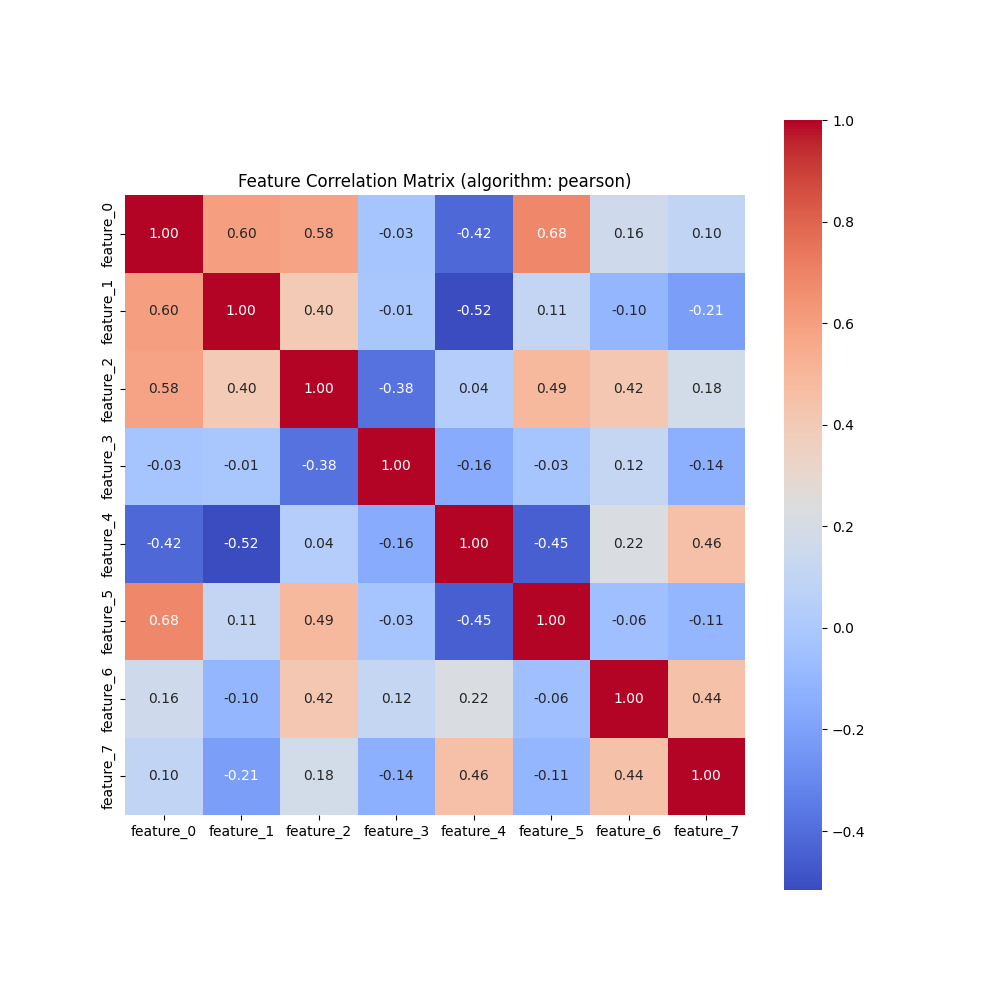
\includegraphics[width=0.8\linewidth]{img/annexes/25_filtered_chunk_extraction_-e_none_-s_activate/Word2vec 0_correlation_matrix.png}} \\
\hline
\end{longtable}


\begin{longtable}{|c|c|}
\caption{Word2vec 1 Feature Engineering Results on 25\_filtered\_chunk\_extraction\_-e\_none\_-s\_activate} \label{tab:25_filtered_chunk_extraction_-e_none_-s_activate_word2vec_1_feature_engineering_results}\\
\hline
Dataset Name & 25\_filtered\_chunk\_extraction\_-e\_none\_-s\_activate \\ \hline
Instance & Word2vec 1 \\ \hline
\multirow{8}{*}{Best Features} & feature\_7 \\ \cline{2-2}
 & feature\_3 \\ \cline{2-2}
 & feature\_4 \\ \cline{2-2}
 & feature\_0 \\ \cline{2-2}
 & feature\_5 \\ \cline{2-2}
 & feature\_6 \\ \cline{2-2}
 & feature\_2 \\ \cline{2-2}
 & feature\_1 \\ \cline{2-2}
\noalign{\vskip 5mm}
\multicolumn{2}{|c|}{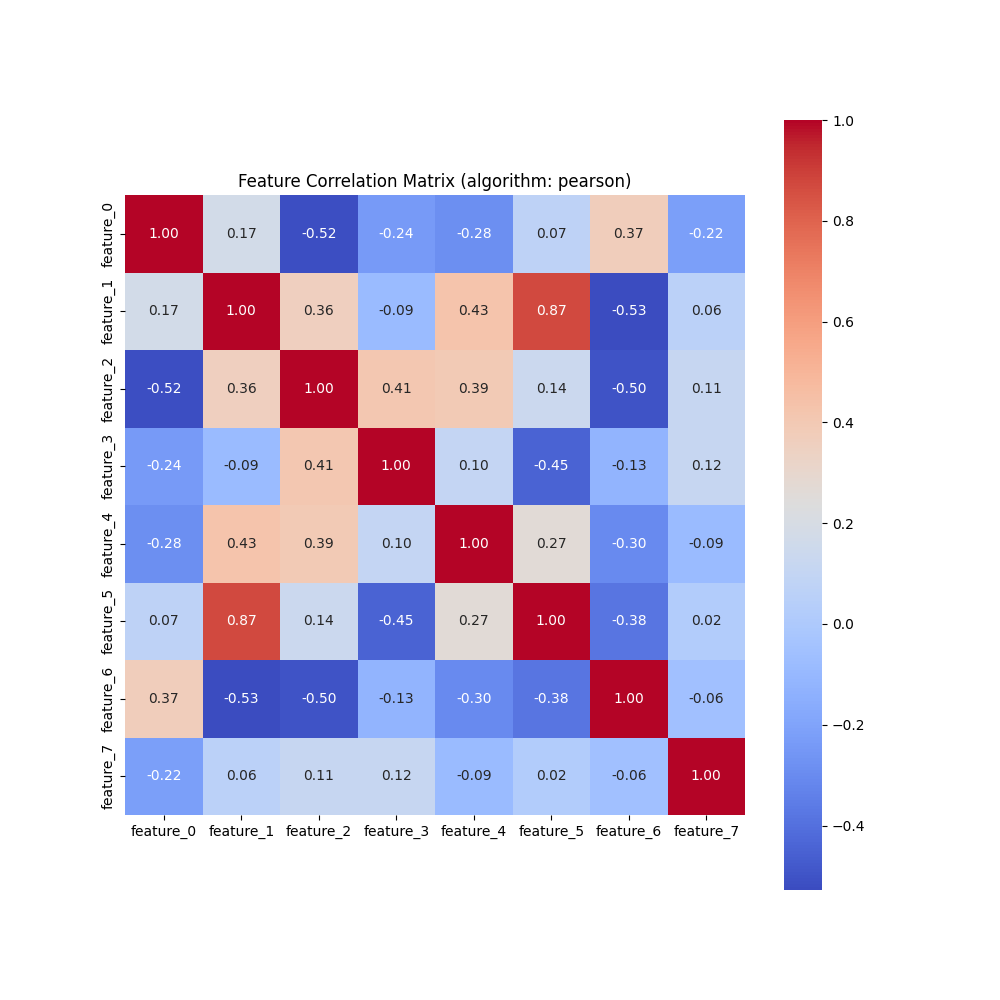
\includegraphics[width=0.8\linewidth]{img/annexes/25_filtered_chunk_extraction_-e_none_-s_activate/Word2vec 1_correlation_matrix.png}} \\
\hline
\end{longtable}


\begin{longtable}{|c|c|}
\caption{Word2vec 2 Feature Engineering Results on 25\_filtered\_chunk\_extraction\_-e\_none\_-s\_activate} \label{tab:25_filtered_chunk_extraction_-e_none_-s_activate_word2vec_2_feature_engineering_results}\\
\hline
Dataset Name & 25\_filtered\_chunk\_extraction\_-e\_none\_-s\_activate \\ \hline
Instance & Word2vec 2 \\ \hline
\multirow{8}{*}{Best Features} & feature\_3 \\ \cline{2-2}
 & feature\_7 \\ \cline{2-2}
 & feature\_5 \\ \cline{2-2}
 & feature\_4 \\ \cline{2-2}
 & feature\_1 \\ \cline{2-2}
 & feature\_6 \\ \cline{2-2}
 & feature\_2 \\ \cline{2-2}
 & feature\_0 \\ \cline{2-2}
\noalign{\vskip 5mm}
\multicolumn{2}{|c|}{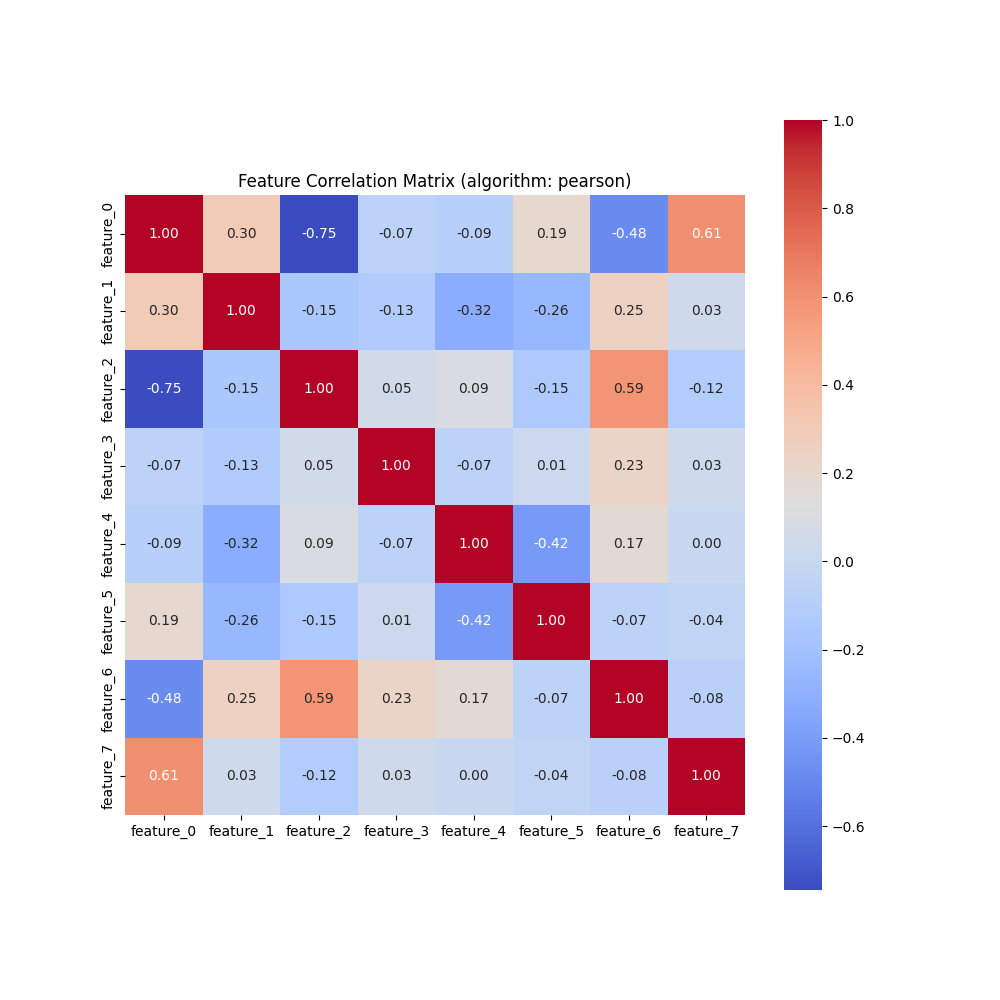
\includegraphics[width=0.8\linewidth]{img/annexes/25_filtered_chunk_extraction_-e_none_-s_activate/Word2vec 2_correlation_matrix.png}} \\
\hline
\end{longtable}


\begin{longtable}{|c|c|}
\caption{Word2vec 3 Feature Engineering Results on 25\_filtered\_chunk\_extraction\_-e\_none\_-s\_activate} \label{tab:25_filtered_chunk_extraction_-e_none_-s_activate_word2vec_3_feature_engineering_results}\\
\hline
Dataset Name & 25\_filtered\_chunk\_extraction\_-e\_none\_-s\_activate \\ \hline
Instance & Word2vec 3 \\ \hline
\multirow{8}{*}{Best Features} & feature\_2 \\ \cline{2-2}
 & feature\_5 \\ \cline{2-2}
 & feature\_3 \\ \cline{2-2}
 & feature\_6 \\ \cline{2-2}
 & feature\_7 \\ \cline{2-2}
 & feature\_4 \\ \cline{2-2}
 & feature\_0 \\ \cline{2-2}
 & feature\_1 \\ \cline{2-2}
\noalign{\vskip 5mm}
\multicolumn{2}{|c|}{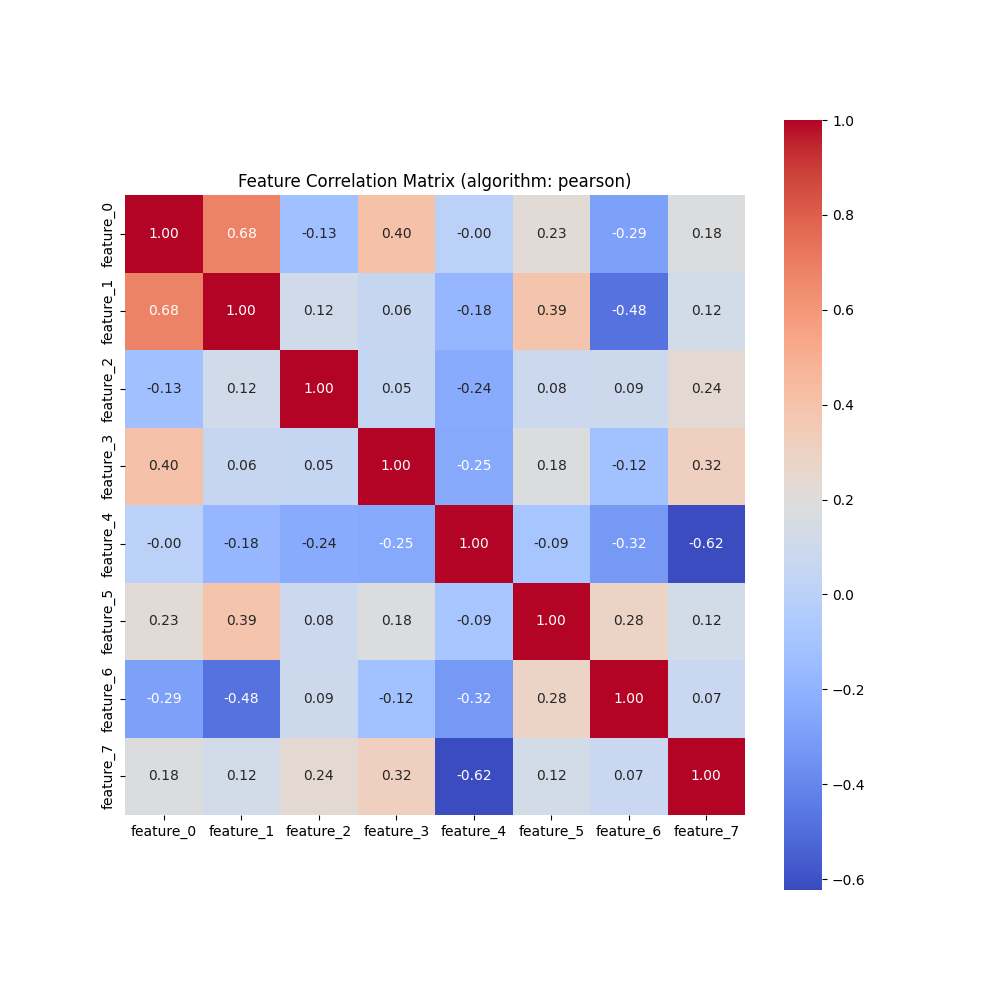
\includegraphics[width=0.8\linewidth]{img/annexes/25_filtered_chunk_extraction_-e_none_-s_activate/Word2vec 3_correlation_matrix.png}} \\
\hline
\end{longtable}


\begin{longtable}{|c|c|}
\caption{Word2vec 4 Feature Engineering Results on 25\_filtered\_chunk\_extraction\_-e\_none\_-s\_activate} \label{tab:25_filtered_chunk_extraction_-e_none_-s_activate_word2vec_4_feature_engineering_results}\\
\hline
Dataset Name & 25\_filtered\_chunk\_extraction\_-e\_none\_-s\_activate \\ \hline
Instance & Word2vec 4 \\ \hline
\multirow{8}{*}{Best Features} & feature\_1 \\ \cline{2-2}
 & feature\_4 \\ \cline{2-2}
 & feature\_10 \\ \cline{2-2}
 & feature\_8 \\ \cline{2-2}
 & feature\_13 \\ \cline{2-2}
 & feature\_15 \\ \cline{2-2}
 & feature\_0 \\ \cline{2-2}
 & feature\_5 \\ \cline{2-2}
\noalign{\vskip 5mm}
\multicolumn{2}{|c|}{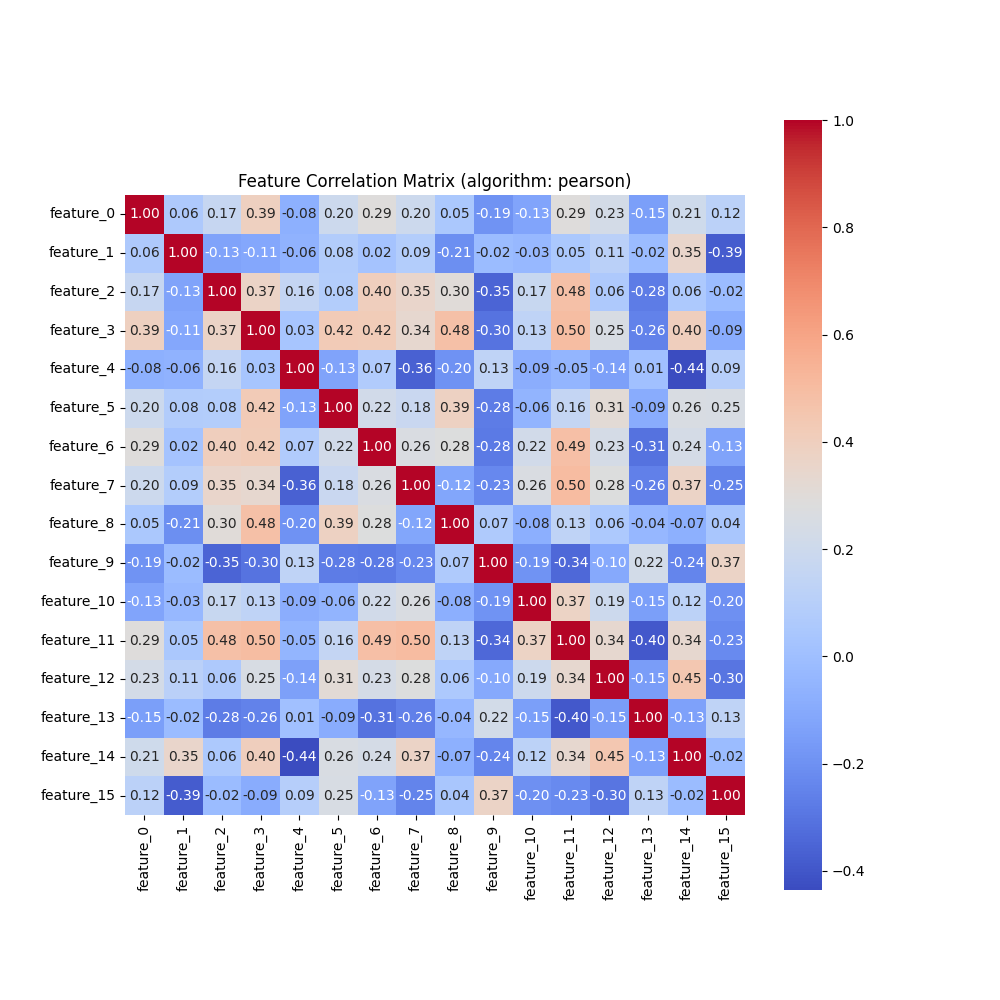
\includegraphics[width=0.8\linewidth]{img/annexes/25_filtered_chunk_extraction_-e_none_-s_activate/Word2vec 4_correlation_matrix.png}} \\
\hline
\end{longtable}


\begin{longtable}{|c|c|}
\caption{Word2vec 5 Feature Engineering Results on 25\_filtered\_chunk\_extraction\_-e\_none\_-s\_activate} \label{tab:25_filtered_chunk_extraction_-e_none_-s_activate_word2vec_5_feature_engineering_results}\\
\hline
Dataset Name & 25\_filtered\_chunk\_extraction\_-e\_none\_-s\_activate \\ \hline
Instance & Word2vec 5 \\ \hline
\multirow{8}{*}{Best Features} & feature\_8 \\ \cline{2-2}
 & feature\_14 \\ \cline{2-2}
 & feature\_12 \\ \cline{2-2}
 & feature\_15 \\ \cline{2-2}
 & feature\_0 \\ \cline{2-2}
 & feature\_11 \\ \cline{2-2}
 & feature\_3 \\ \cline{2-2}
 & feature\_2 \\ \cline{2-2}
\noalign{\vskip 5mm}
\multicolumn{2}{|c|}{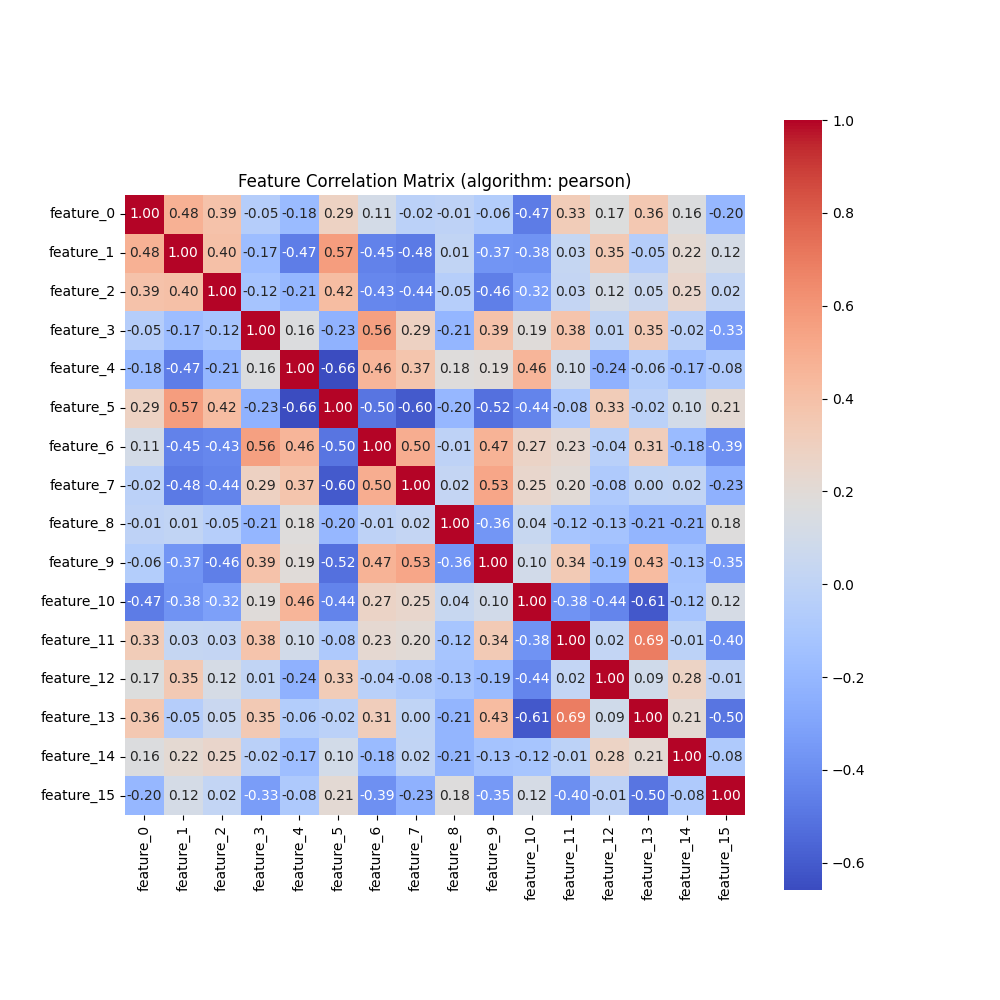
\includegraphics[width=0.8\linewidth]{img/annexes/25_filtered_chunk_extraction_-e_none_-s_activate/Word2vec 5_correlation_matrix.png}} \\
\hline
\end{longtable}


\begin{longtable}{|c|c|}
\caption{Word2vec 6 Feature Engineering Results on 25\_filtered\_chunk\_extraction\_-e\_none\_-s\_activate} \label{tab:25_filtered_chunk_extraction_-e_none_-s_activate_word2vec_6_feature_engineering_results}\\
\hline
Dataset Name & 25\_filtered\_chunk\_extraction\_-e\_none\_-s\_activate \\ \hline
Instance & Word2vec 6 \\ \hline
\multirow{8}{*}{Best Features} & feature\_13 \\ \cline{2-2}
 & feature\_1 \\ \cline{2-2}
 & feature\_9 \\ \cline{2-2}
 & feature\_3 \\ \cline{2-2}
 & feature\_10 \\ \cline{2-2}
 & feature\_7 \\ \cline{2-2}
 & feature\_8 \\ \cline{2-2}
 & feature\_4 \\ \cline{2-2}
\noalign{\vskip 5mm}
\multicolumn{2}{|c|}{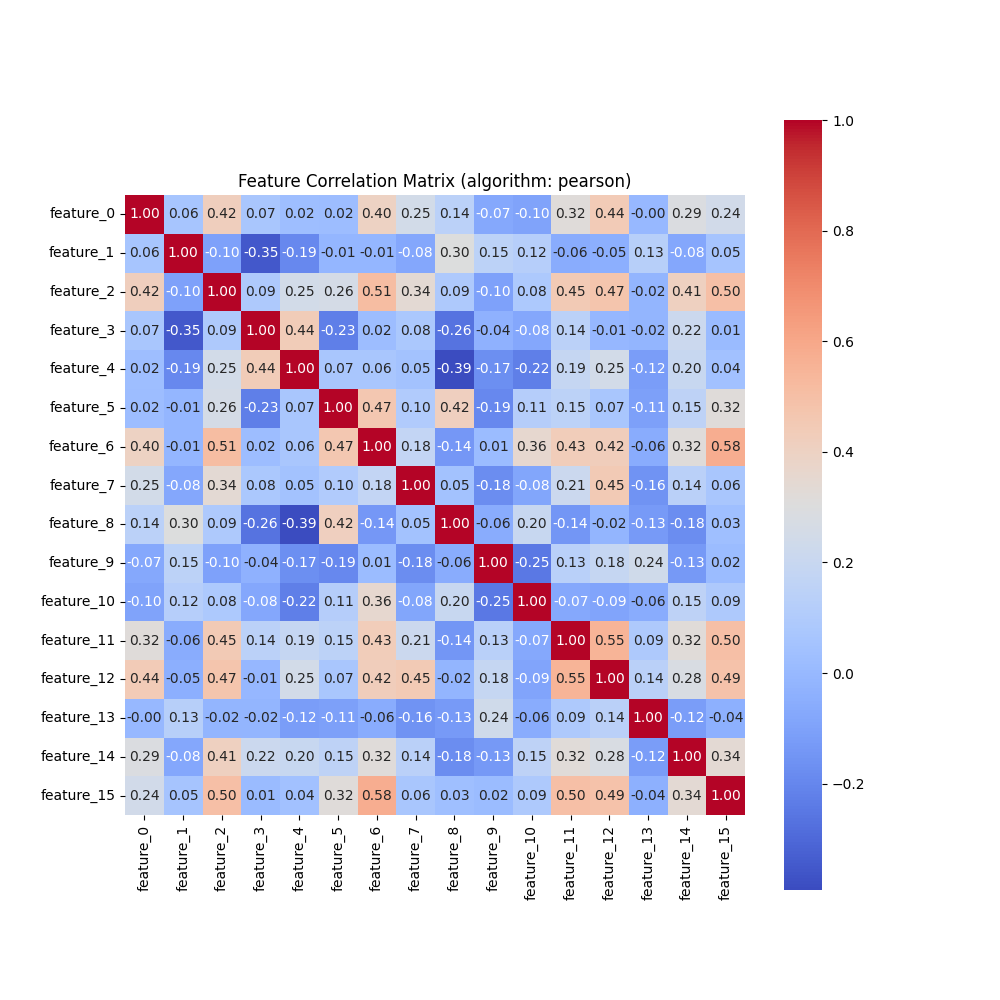
\includegraphics[width=0.8\linewidth]{img/annexes/25_filtered_chunk_extraction_-e_none_-s_activate/Word2vec 6_correlation_matrix.png}} \\
\hline
\end{longtable}


\begin{longtable}{|c|c|}
\caption{Word2vec 7 Feature Engineering Results on 25\_filtered\_chunk\_extraction\_-e\_none\_-s\_activate} \label{tab:25_filtered_chunk_extraction_-e_none_-s_activate_word2vec_7_feature_engineering_results}\\
\hline
Dataset Name & 25\_filtered\_chunk\_extraction\_-e\_none\_-s\_activate \\ \hline
Instance & Word2vec 7 \\ \hline
\multirow{8}{*}{Best Features} & feature\_2 \\ \cline{2-2}
 & feature\_15 \\ \cline{2-2}
 & feature\_8 \\ \cline{2-2}
 & feature\_14 \\ \cline{2-2}
 & feature\_10 \\ \cline{2-2}
 & feature\_1 \\ \cline{2-2}
 & feature\_0 \\ \cline{2-2}
 & feature\_13 \\ \cline{2-2}
\noalign{\vskip 5mm}
\multicolumn{2}{|c|}{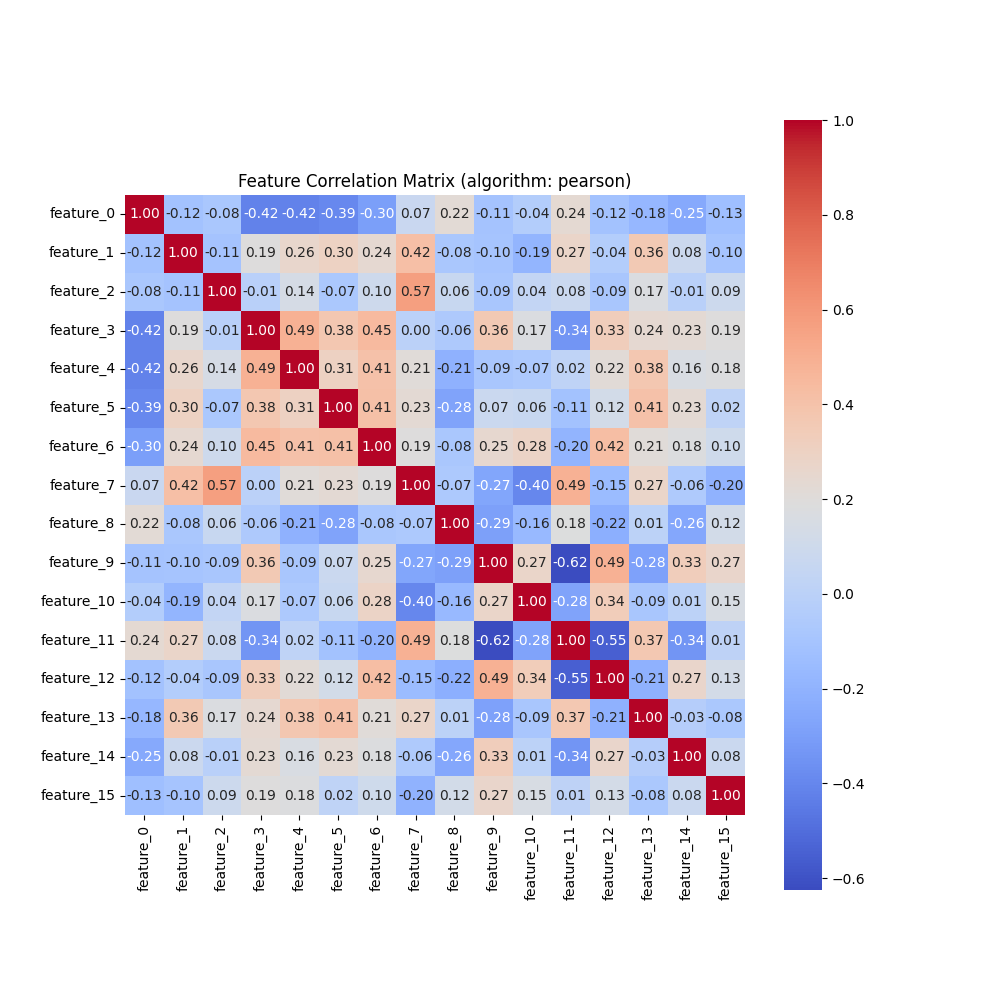
\includegraphics[width=0.8\linewidth]{img/annexes/25_filtered_chunk_extraction_-e_none_-s_activate/Word2vec 7_correlation_matrix.png}} \\
\hline
\end{longtable}


\begin{longtable}{|c|c|}
\caption{Word2vec 8 Feature Engineering Results on 25\_filtered\_chunk\_extraction\_-e\_none\_-s\_activate} \label{tab:25_filtered_chunk_extraction_-e_none_-s_activate_word2vec_8_feature_engineering_results}\\
\hline
Dataset Name & 25\_filtered\_chunk\_extraction\_-e\_none\_-s\_activate \\ \hline
Instance & Word2vec 8 \\ \hline
\multirow{8}{*}{Best Features} & feature\_3 \\ \cline{2-2}
 & feature\_31 \\ \cline{2-2}
 & feature\_62 \\ \cline{2-2}
 & feature\_78 \\ \cline{2-2}
 & feature\_93 \\ \cline{2-2}
 & feature\_11 \\ \cline{2-2}
 & feature\_32 \\ \cline{2-2}
 & feature\_61 \\ \cline{2-2}
\noalign{\vskip 5mm}
\multicolumn{2}{|c|}{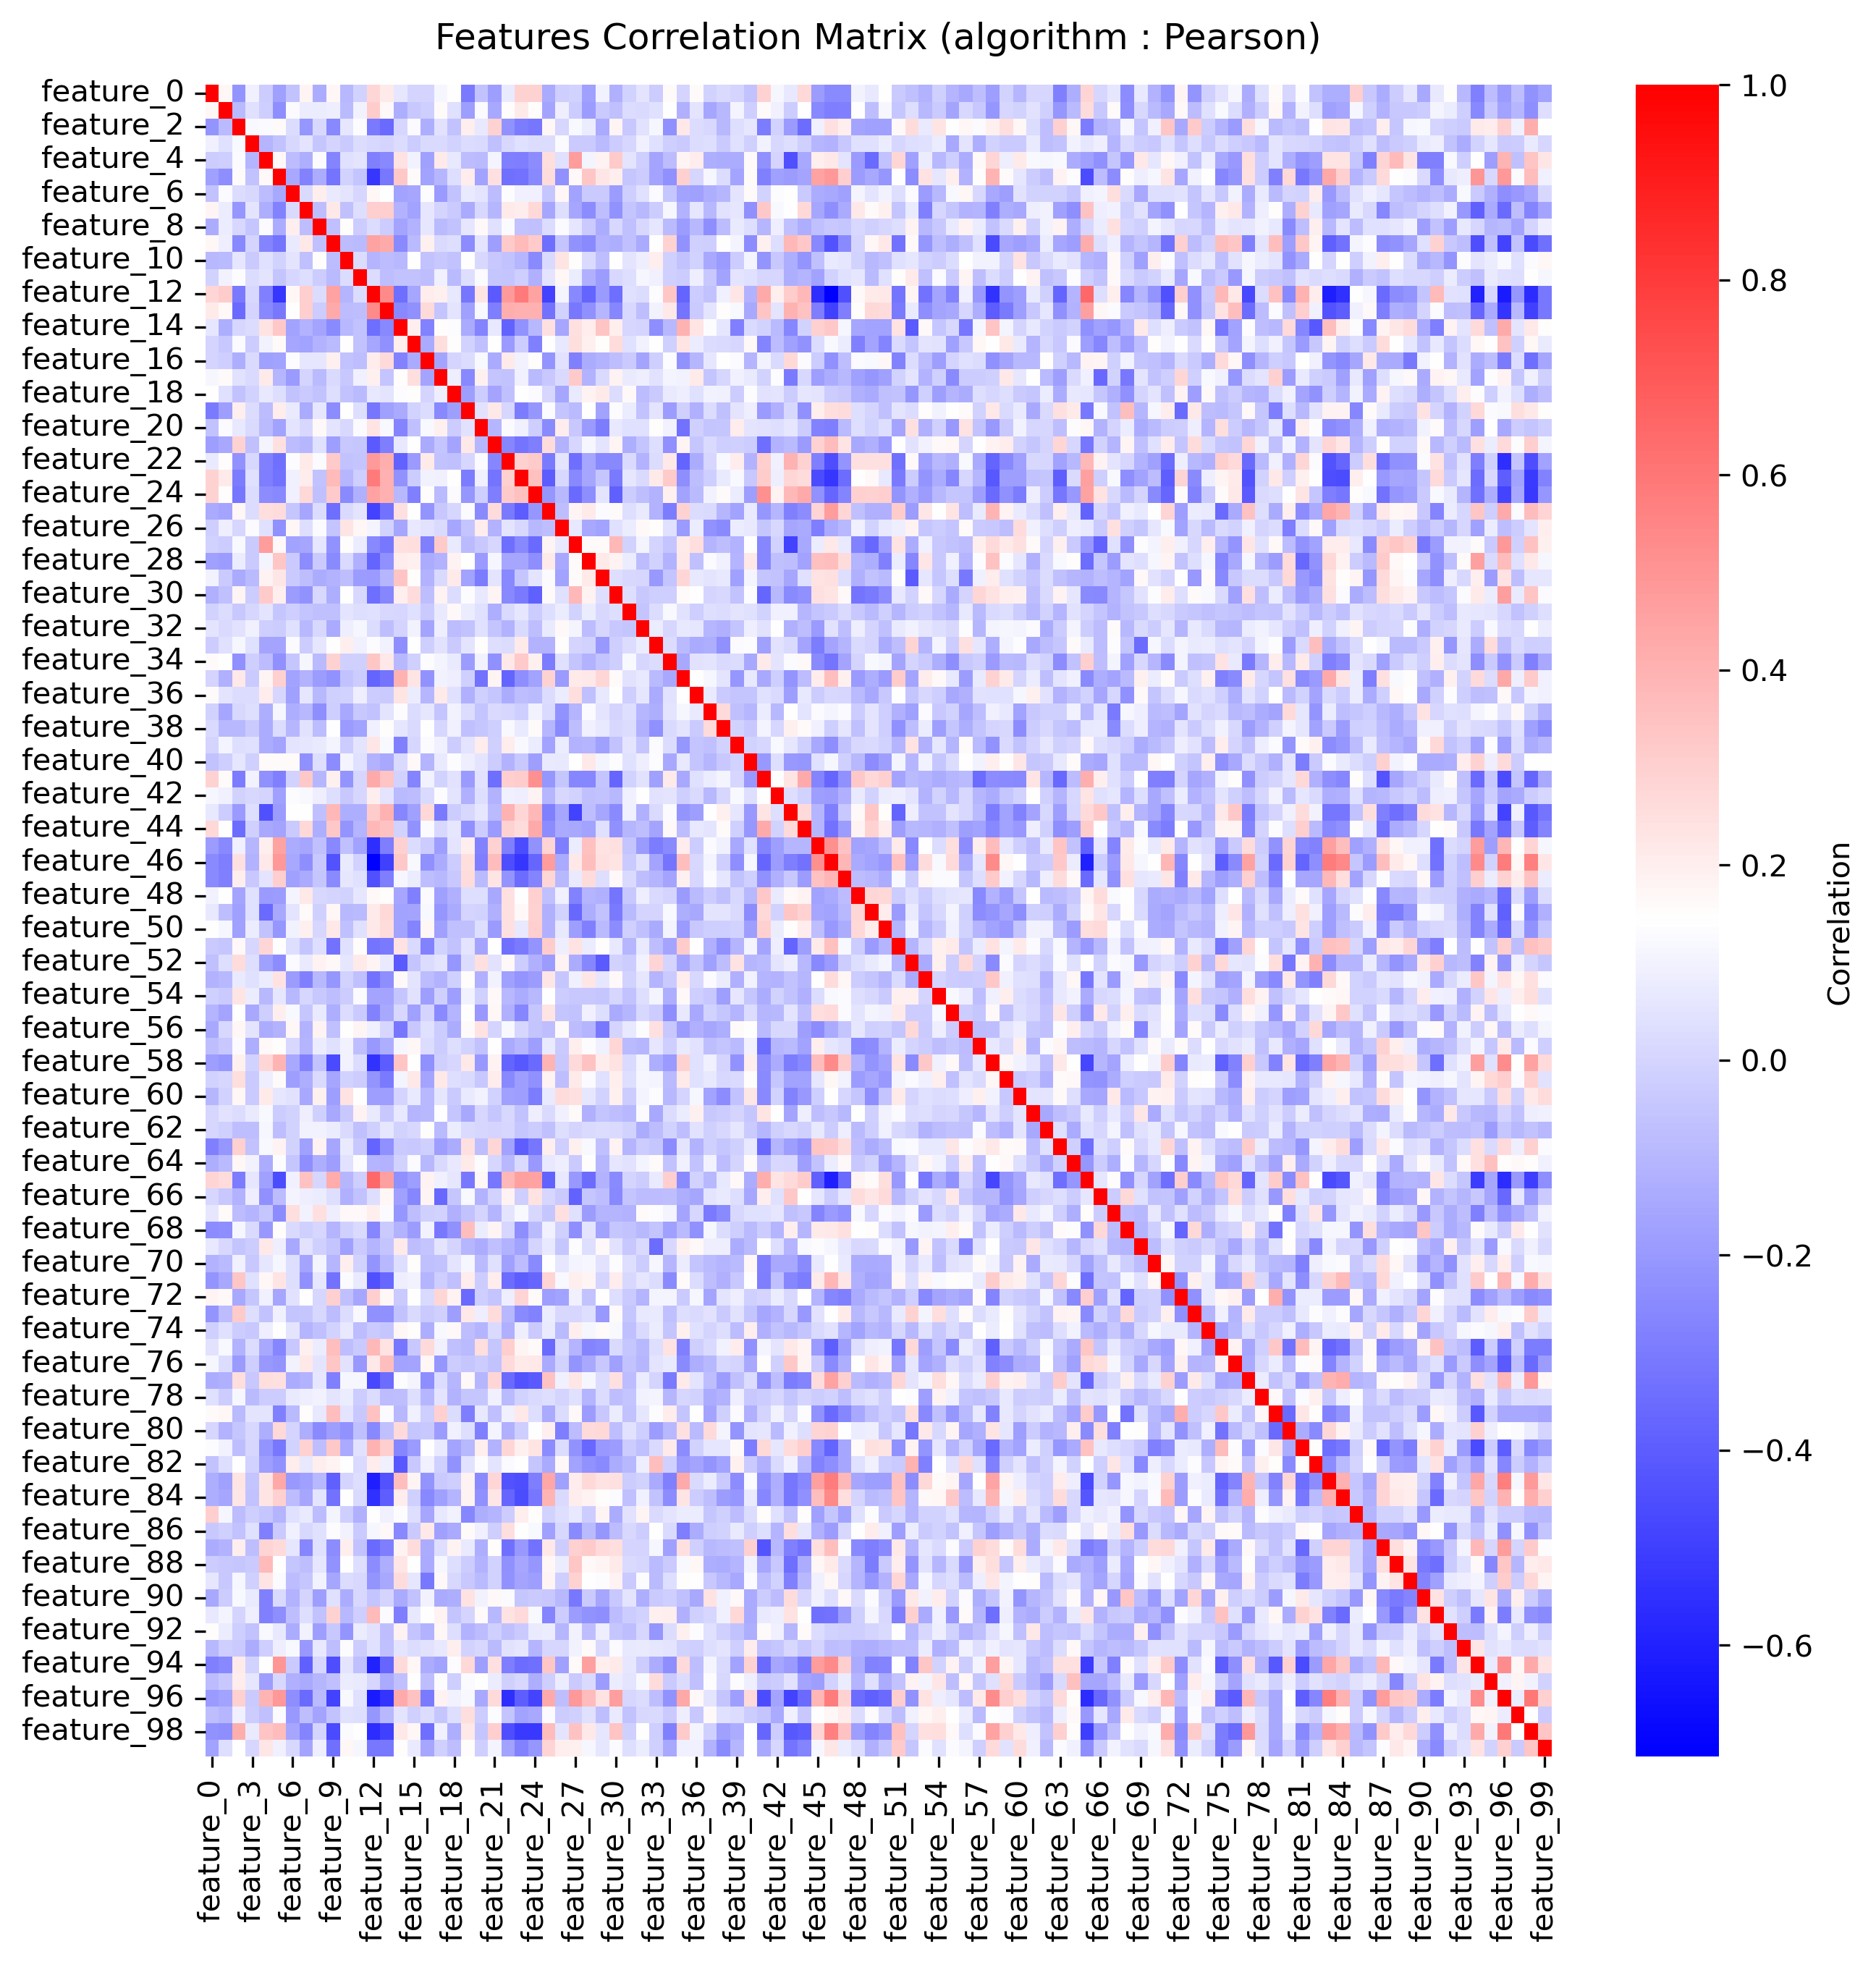
\includegraphics[width=0.8\linewidth]{img/annexes/25_filtered_chunk_extraction_-e_none_-s_activate/Word2vec 8_correlation_matrix.png}} \\
\hline
\end{longtable}


\begin{longtable}{|c|c|}
\caption{Word2vec 9 Feature Engineering Results on 25\_filtered\_chunk\_extraction\_-e\_none\_-s\_activate} \label{tab:25_filtered_chunk_extraction_-e_none_-s_activate_word2vec_9_feature_engineering_results}\\
\hline
Dataset Name & 25\_filtered\_chunk\_extraction\_-e\_none\_-s\_activate \\ \hline
Instance & Word2vec 9 \\ \hline
\multirow{8}{*}{Best Features} & feature\_0 \\ \cline{2-2}
 & feature\_36 \\ \cline{2-2}
 & feature\_94 \\ \cline{2-2}
 & feature\_70 \\ \cline{2-2}
 & feature\_69 \\ \cline{2-2}
 & feature\_22 \\ \cline{2-2}
 & feature\_84 \\ \cline{2-2}
 & feature\_37 \\ \cline{2-2}
\noalign{\vskip 5mm}
\multicolumn{2}{|c|}{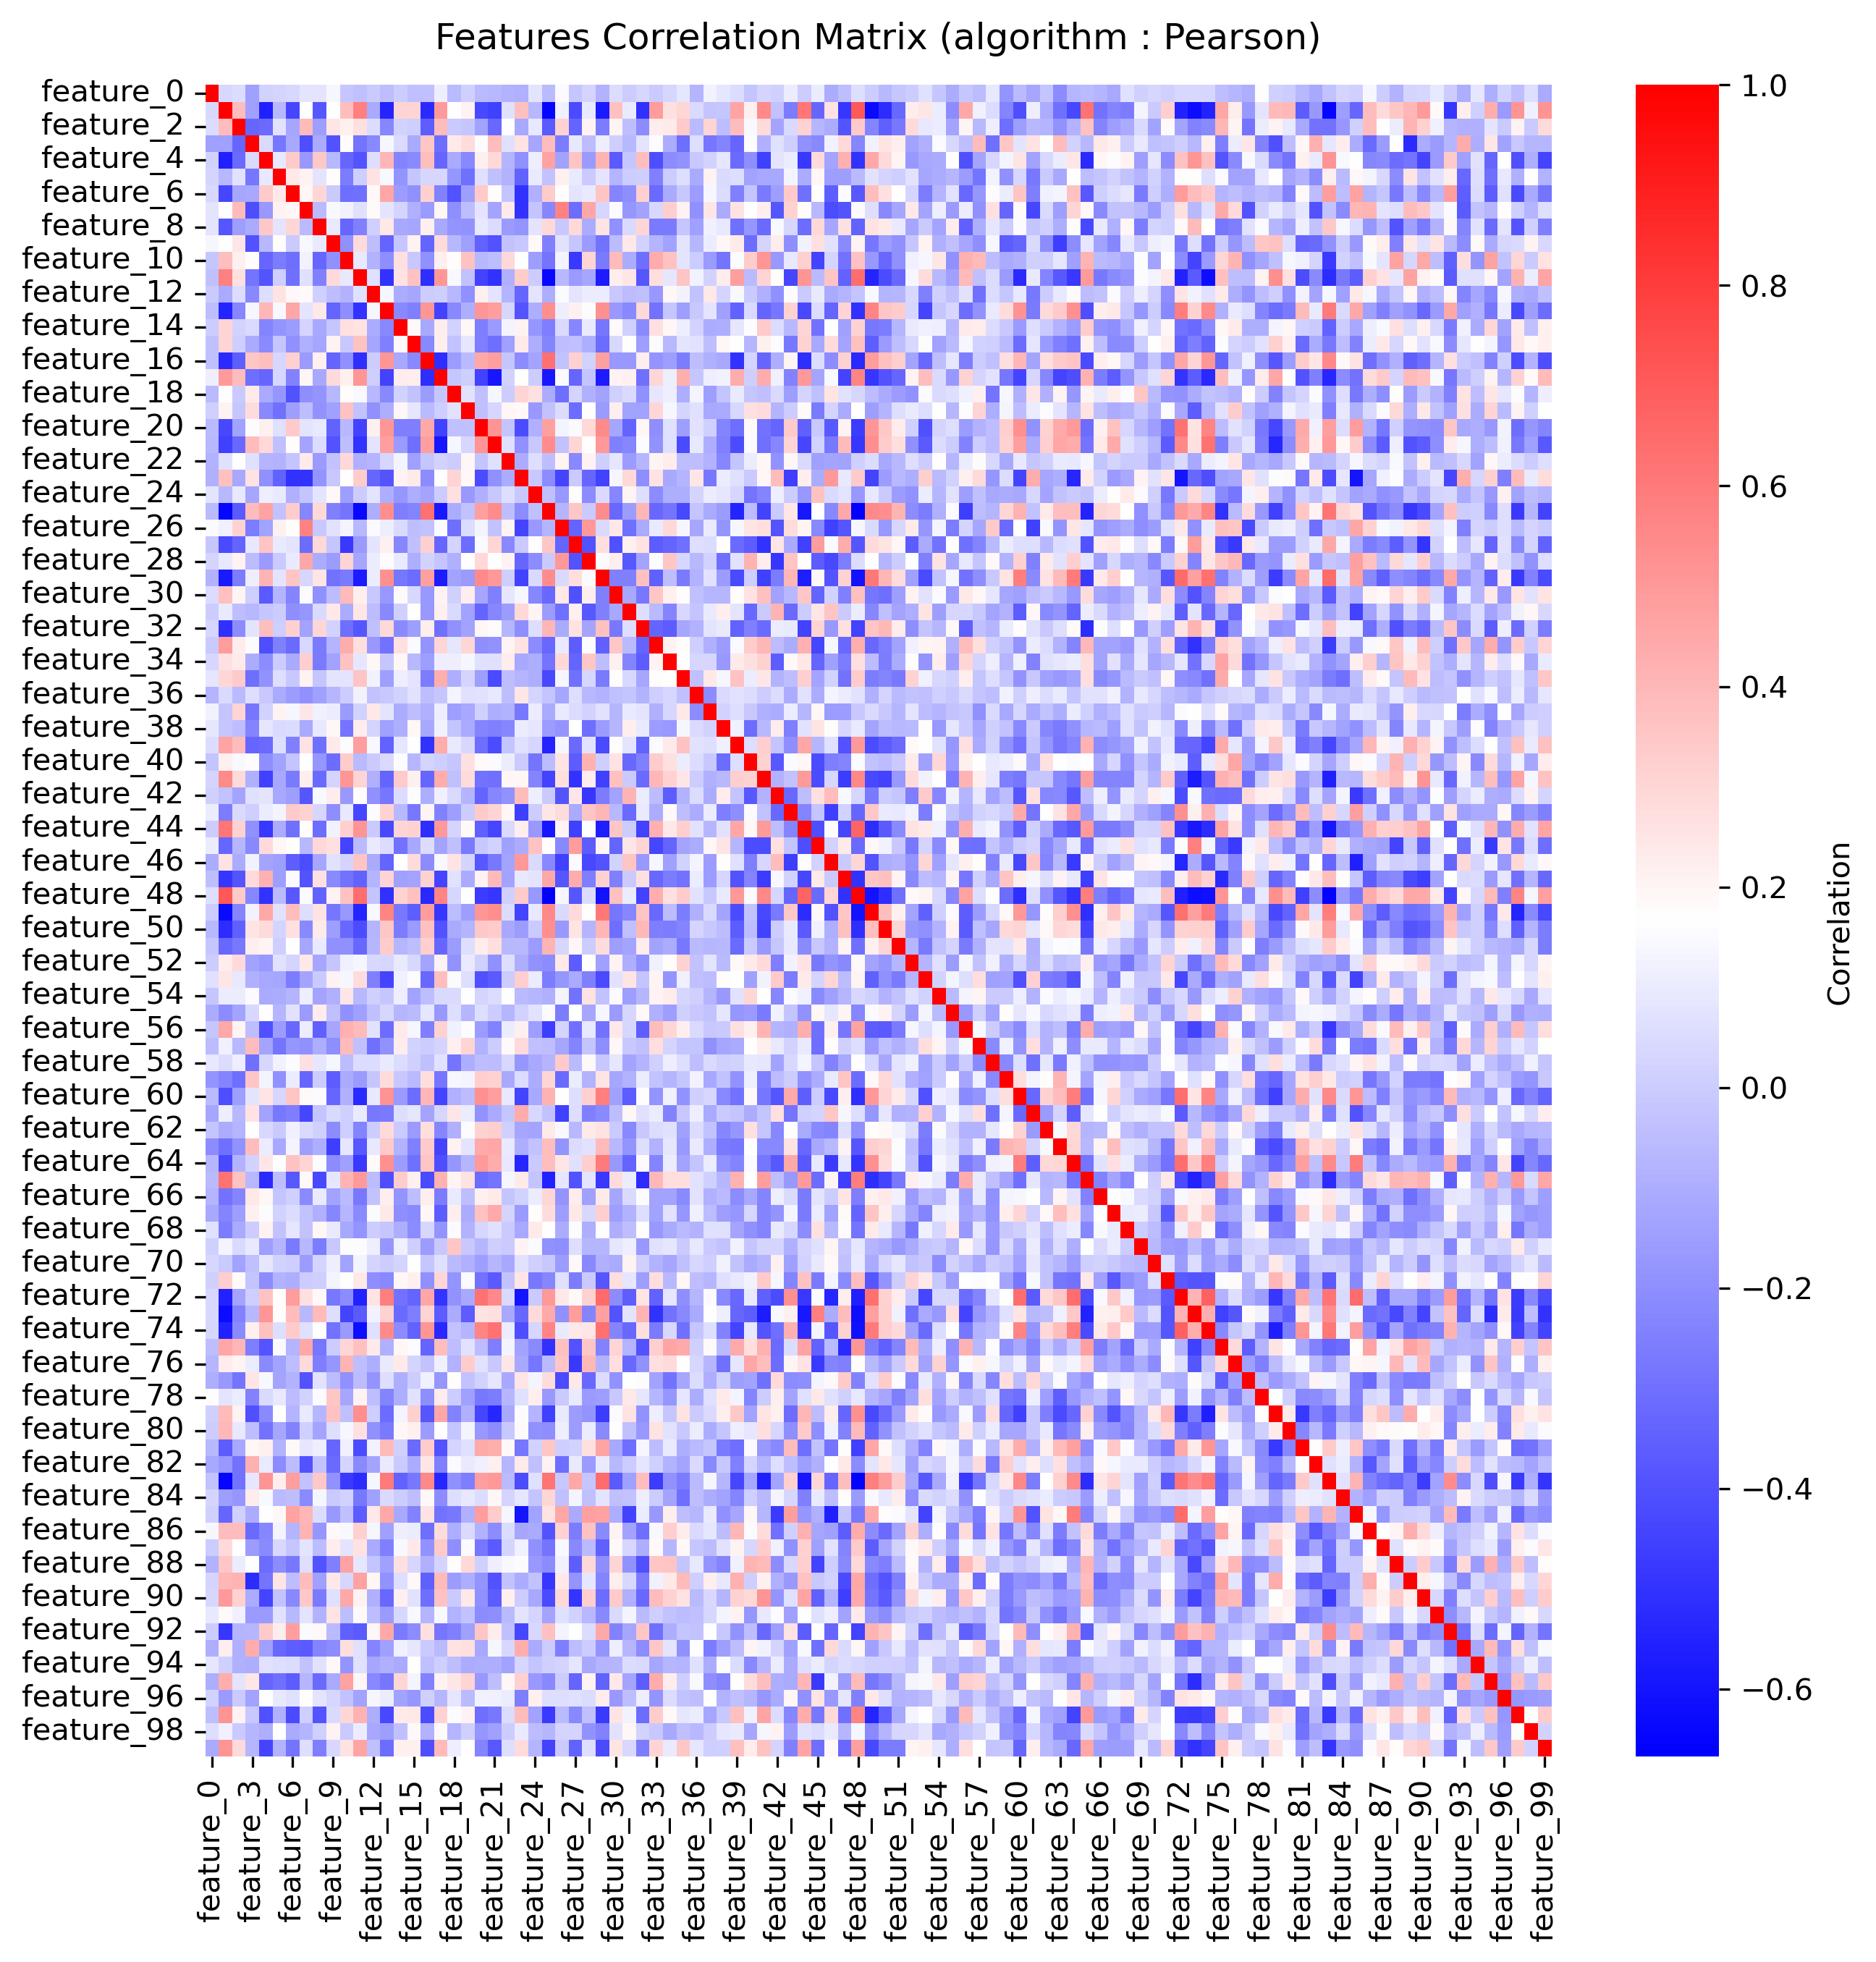
\includegraphics[width=0.8\linewidth]{img/annexes/25_filtered_chunk_extraction_-e_none_-s_activate/Word2vec 9_correlation_matrix.png}} \\
\hline
\end{longtable}


\subsection{26\_filtered\_chunk\_extraction\_-e\_only-max-entropy\_-s\_none}

\begin{longtable}{|c|c|}
\caption{Transformers 0 Feature Engineering Results on 26\_filtered\_chunk\_extraction\_-e\_only-max-entropy\_-s\_none} \label{tab:26_filtered_chunk_extraction_-e_only-max-entropy_-s_none_transformers_0_feature_engineering_results}\\
\hline
Dataset Name & 26\_filtered\_chunk\_extraction\_-e\_only-max-entropy\_-s\_none \\ \hline
Instance & Transformers 0 \\ \hline
\multirow{8}{*}{Best Features} & embedded\_6 \\ \cline{2-2}
 & embedded\_3 \\ \cline{2-2}
 & embedded\_0 \\ \cline{2-2}
 & embedded\_5 \\ \cline{2-2}
 & embedded\_4 \\ \cline{2-2}
 & embedded\_1 \\ \cline{2-2}
 & embedded\_2 \\ \cline{2-2}
 & embedded\_7 \\ \cline{2-2}
\noalign{\vskip 5mm}
\multicolumn{2}{|c|}{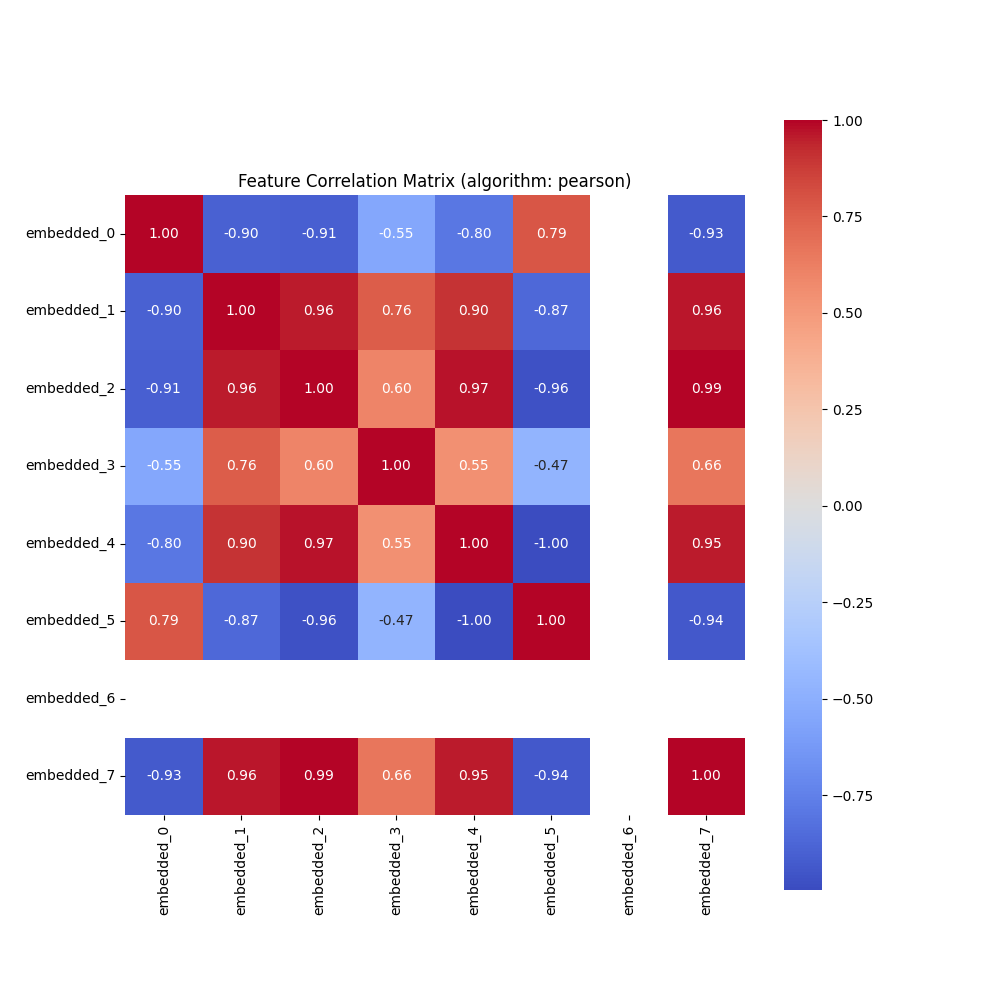
\includegraphics[width=0.8\linewidth]{img/annexes/26_filtered_chunk_extraction_-e_only-max-entropy_-s_none/Transformers 0_correlation_matrix.png}} \\
\hline
\end{longtable}


\begin{longtable}{|c|c|}
\caption{Transformers 1 Feature Engineering Results on 26\_filtered\_chunk\_extraction\_-e\_only-max-entropy\_-s\_none} \label{tab:26_filtered_chunk_extraction_-e_only-max-entropy_-s_none_transformers_1_feature_engineering_results}\\
\hline
Dataset Name & 26\_filtered\_chunk\_extraction\_-e\_only-max-entropy\_-s\_none \\ \hline
Instance & Transformers 1 \\ \hline
\multirow{8}{*}{Best Features} & embedded\_2 \\ \cline{2-2}
 & embedded\_8 \\ \cline{2-2}
 & embedded\_14 \\ \cline{2-2}
 & embedded\_5 \\ \cline{2-2}
 & embedded\_6 \\ \cline{2-2}
 & embedded\_1 \\ \cline{2-2}
 & embedded\_13 \\ \cline{2-2}
 & embedded\_15 \\ \cline{2-2}
\noalign{\vskip 5mm}
\multicolumn{2}{|c|}{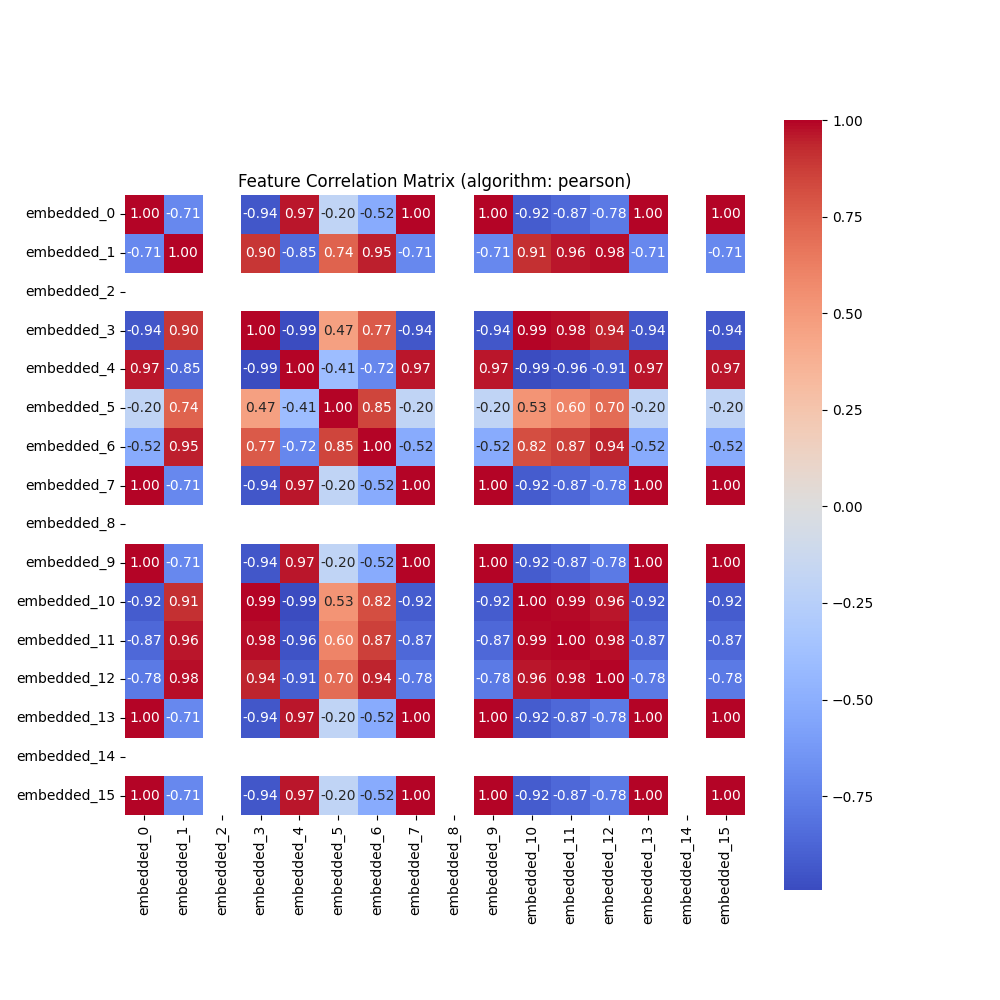
\includegraphics[width=0.8\linewidth]{img/annexes/26_filtered_chunk_extraction_-e_only-max-entropy_-s_none/Transformers 1_correlation_matrix.png}} \\
\hline
\end{longtable}


\begin{longtable}{|c|c|}
\caption{Word2vec 0 Feature Engineering Results on 26\_filtered\_chunk\_extraction\_-e\_only-max-entropy\_-s\_none} \label{tab:26_filtered_chunk_extraction_-e_only-max-entropy_-s_none_word2vec_0_feature_engineering_results}\\
\hline
Dataset Name & 26\_filtered\_chunk\_extraction\_-e\_only-max-entropy\_-s\_none \\ \hline
Instance & Word2vec 0 \\ \hline
\multirow{8}{*}{Best Features} & feature\_3 \\ \cline{2-2}
 & feature\_5 \\ \cline{2-2}
 & feature\_2 \\ \cline{2-2}
 & feature\_6 \\ \cline{2-2}
 & feature\_4 \\ \cline{2-2}
 & feature\_7 \\ \cline{2-2}
 & feature\_1 \\ \cline{2-2}
 & feature\_0 \\ \cline{2-2}
\noalign{\vskip 5mm}
\multicolumn{2}{|c|}{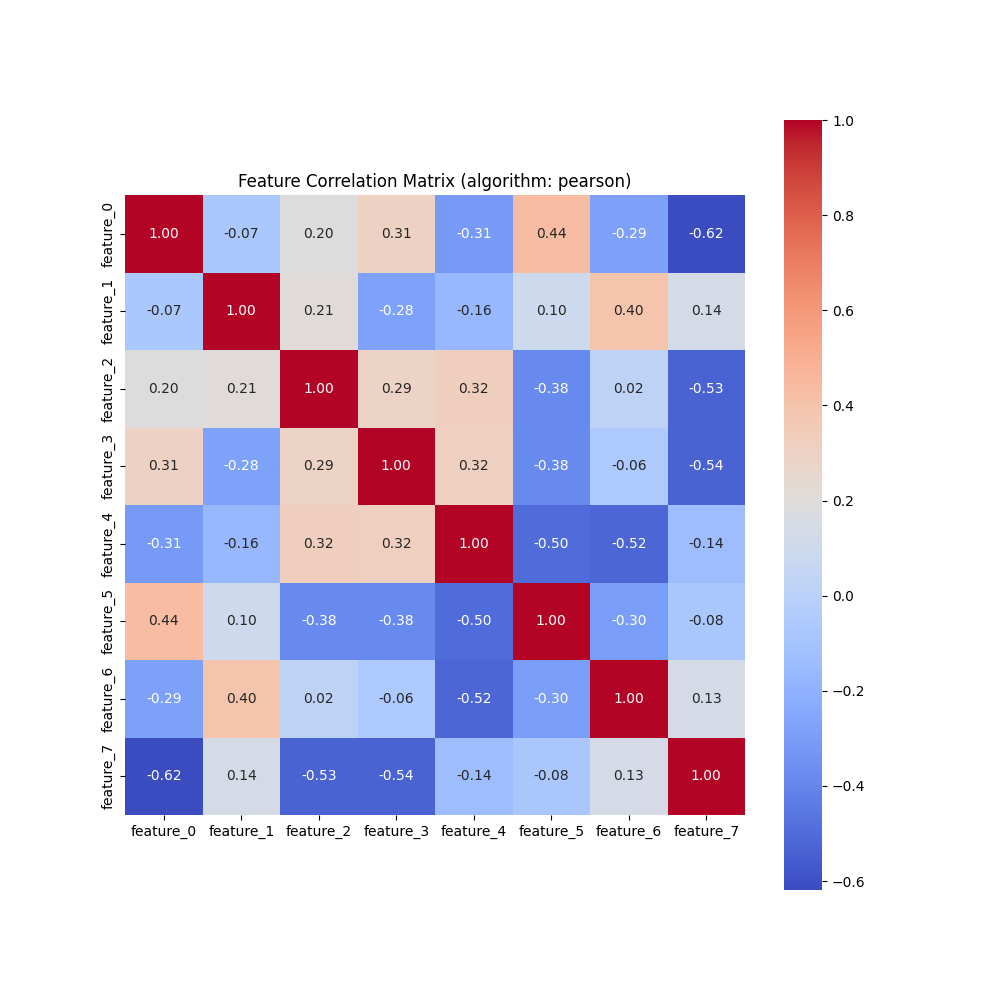
\includegraphics[width=0.8\linewidth]{img/annexes/26_filtered_chunk_extraction_-e_only-max-entropy_-s_none/Word2vec 0_correlation_matrix.png}} \\
\hline
\end{longtable}


\begin{longtable}{|c|c|}
\caption{Word2vec 1 Feature Engineering Results on 26\_filtered\_chunk\_extraction\_-e\_only-max-entropy\_-s\_none} \label{tab:26_filtered_chunk_extraction_-e_only-max-entropy_-s_none_word2vec_1_feature_engineering_results}\\
\hline
Dataset Name & 26\_filtered\_chunk\_extraction\_-e\_only-max-entropy\_-s\_none \\ \hline
Instance & Word2vec 1 \\ \hline
\multirow{8}{*}{Best Features} & feature\_4 \\ \cline{2-2}
 & feature\_5 \\ \cline{2-2}
 & feature\_6 \\ \cline{2-2}
 & feature\_7 \\ \cline{2-2}
 & feature\_2 \\ \cline{2-2}
 & feature\_3 \\ \cline{2-2}
 & feature\_0 \\ \cline{2-2}
 & feature\_1 \\ \cline{2-2}
\noalign{\vskip 5mm}
\multicolumn{2}{|c|}{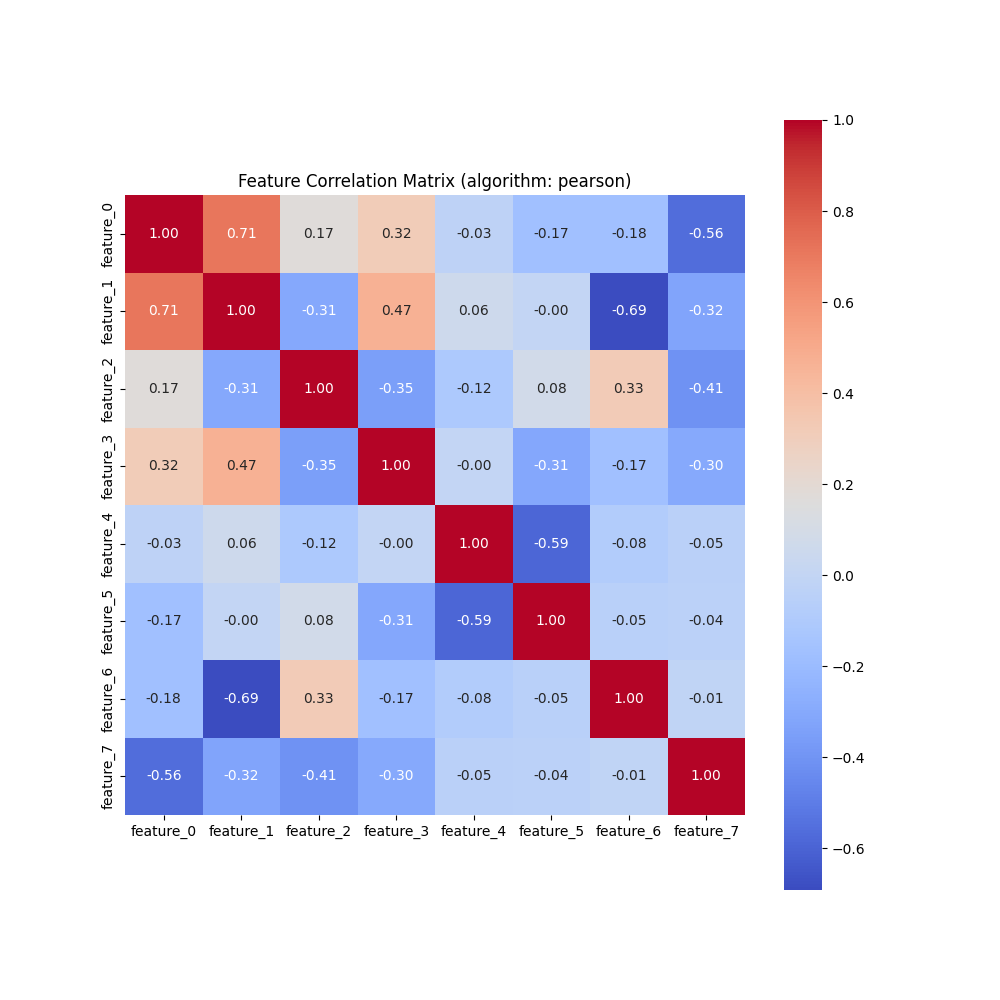
\includegraphics[width=0.8\linewidth]{img/annexes/26_filtered_chunk_extraction_-e_only-max-entropy_-s_none/Word2vec 1_correlation_matrix.png}} \\
\hline
\end{longtable}


\begin{longtable}{|c|c|}
\caption{Word2vec 2 Feature Engineering Results on 26\_filtered\_chunk\_extraction\_-e\_only-max-entropy\_-s\_none} \label{tab:26_filtered_chunk_extraction_-e_only-max-entropy_-s_none_word2vec_2_feature_engineering_results}\\
\hline
Dataset Name & 26\_filtered\_chunk\_extraction\_-e\_only-max-entropy\_-s\_none \\ \hline
Instance & Word2vec 2 \\ \hline
\multirow{8}{*}{Best Features} & feature\_2 \\ \cline{2-2}
 & feature\_0 \\ \cline{2-2}
 & feature\_3 \\ \cline{2-2}
 & feature\_6 \\ \cline{2-2}
 & feature\_5 \\ \cline{2-2}
 & feature\_4 \\ \cline{2-2}
 & feature\_7 \\ \cline{2-2}
 & feature\_1 \\ \cline{2-2}
\noalign{\vskip 5mm}
\multicolumn{2}{|c|}{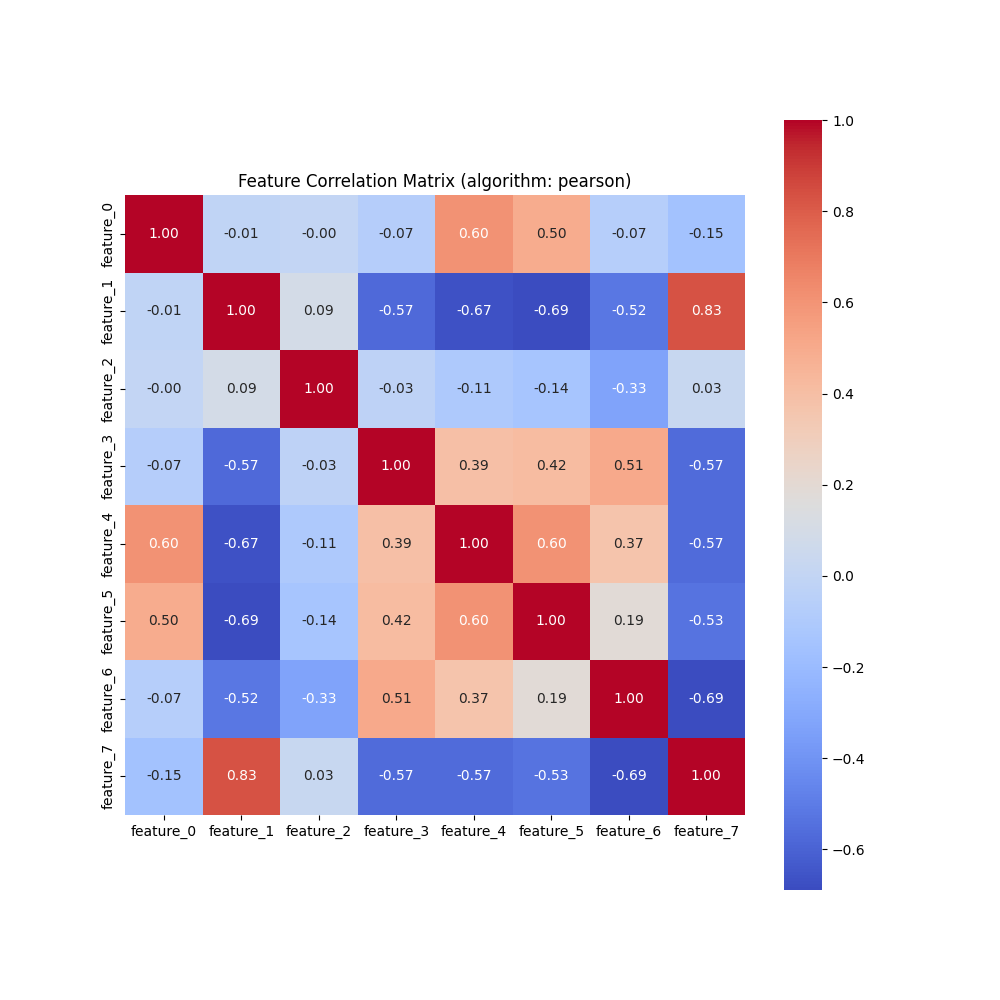
\includegraphics[width=0.8\linewidth]{img/annexes/26_filtered_chunk_extraction_-e_only-max-entropy_-s_none/Word2vec 2_correlation_matrix.png}} \\
\hline
\end{longtable}


\begin{longtable}{|c|c|}
\caption{Word2vec 3 Feature Engineering Results on 26\_filtered\_chunk\_extraction\_-e\_only-max-entropy\_-s\_none} \label{tab:26_filtered_chunk_extraction_-e_only-max-entropy_-s_none_word2vec_3_feature_engineering_results}\\
\hline
Dataset Name & 26\_filtered\_chunk\_extraction\_-e\_only-max-entropy\_-s\_none \\ \hline
Instance & Word2vec 3 \\ \hline
\multirow{8}{*}{Best Features} & feature\_4 \\ \cline{2-2}
 & feature\_2 \\ \cline{2-2}
 & feature\_7 \\ \cline{2-2}
 & feature\_0 \\ \cline{2-2}
 & feature\_5 \\ \cline{2-2}
 & feature\_6 \\ \cline{2-2}
 & feature\_3 \\ \cline{2-2}
 & feature\_1 \\ \cline{2-2}
\noalign{\vskip 5mm}
\multicolumn{2}{|c|}{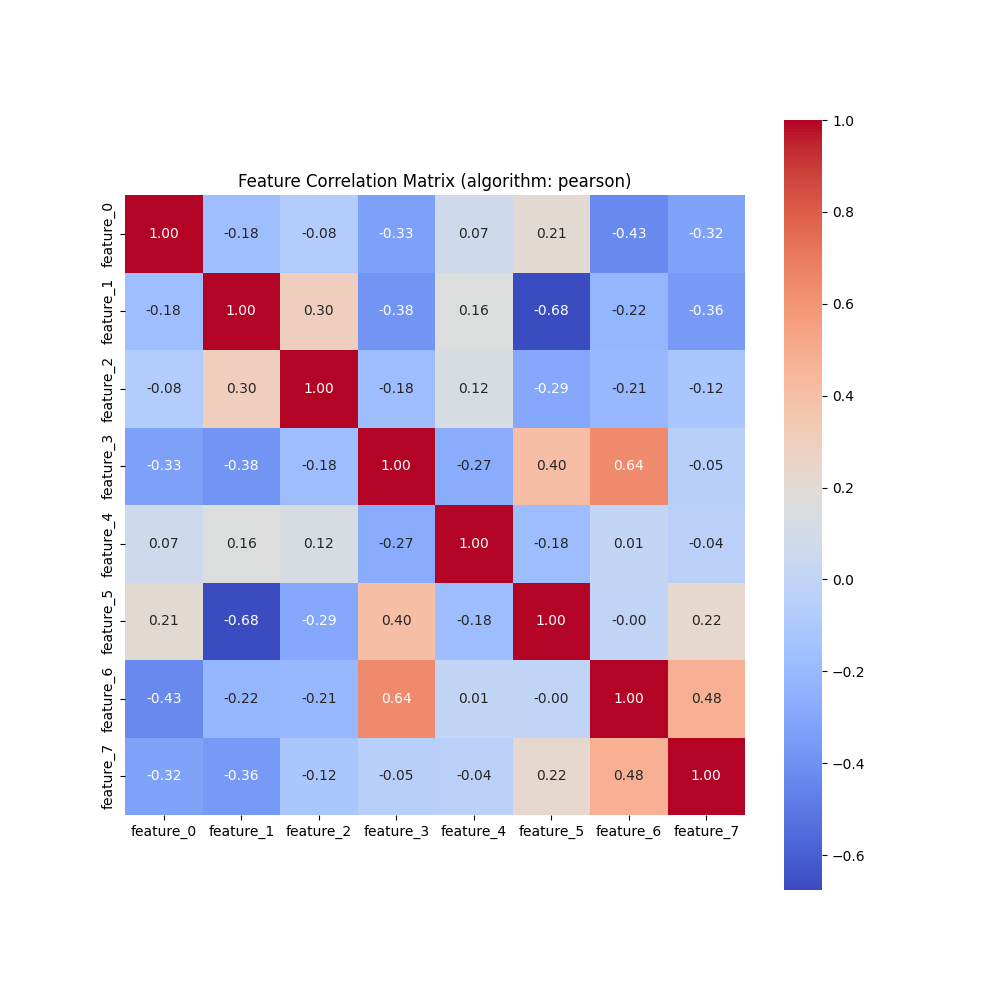
\includegraphics[width=0.8\linewidth]{img/annexes/26_filtered_chunk_extraction_-e_only-max-entropy_-s_none/Word2vec 3_correlation_matrix.png}} \\
\hline
\end{longtable}


\begin{longtable}{|c|c|}
\caption{Word2vec 4 Feature Engineering Results on 26\_filtered\_chunk\_extraction\_-e\_only-max-entropy\_-s\_none} \label{tab:26_filtered_chunk_extraction_-e_only-max-entropy_-s_none_word2vec_4_feature_engineering_results}\\
\hline
Dataset Name & 26\_filtered\_chunk\_extraction\_-e\_only-max-entropy\_-s\_none \\ \hline
Instance & Word2vec 4 \\ \hline
\multirow{8}{*}{Best Features} & feature\_10 \\ \cline{2-2}
 & feature\_0 \\ \cline{2-2}
 & feature\_5 \\ \cline{2-2}
 & feature\_12 \\ \cline{2-2}
 & feature\_11 \\ \cline{2-2}
 & feature\_7 \\ \cline{2-2}
 & feature\_6 \\ \cline{2-2}
 & feature\_3 \\ \cline{2-2}
\noalign{\vskip 5mm}
\multicolumn{2}{|c|}{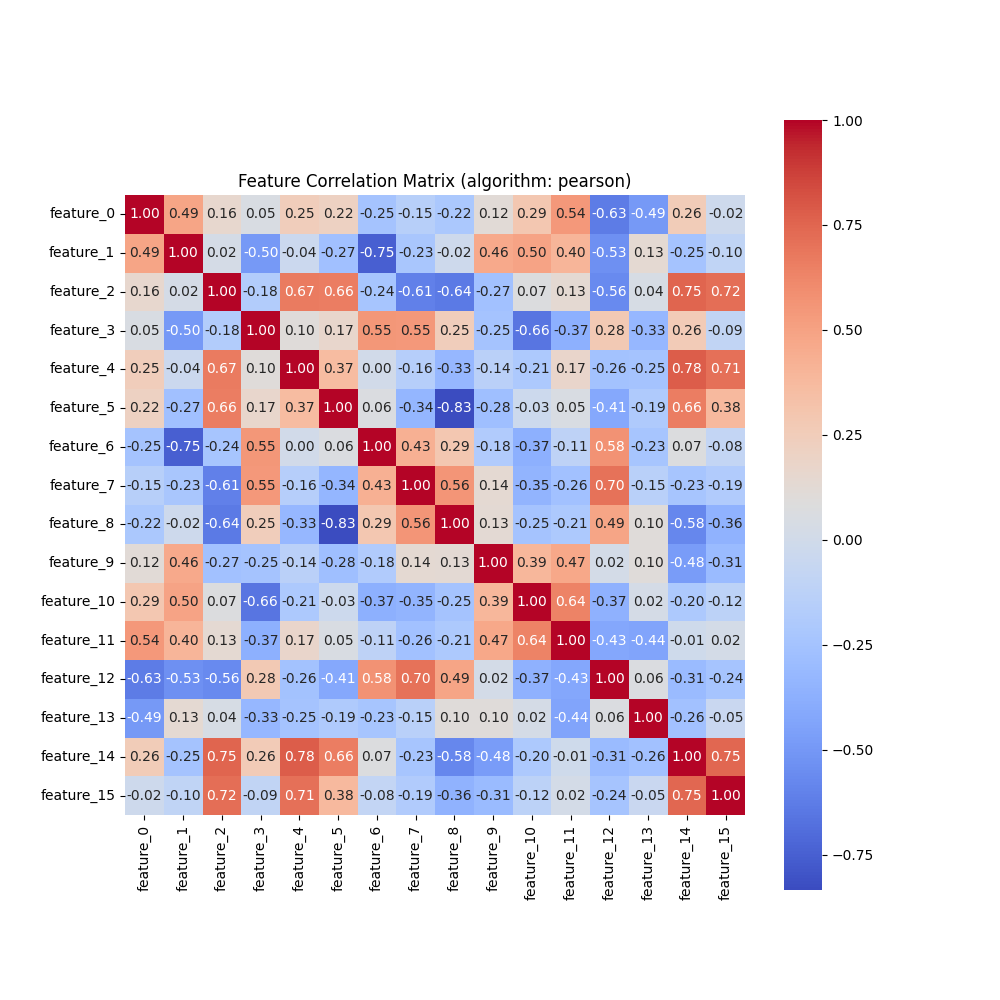
\includegraphics[width=0.8\linewidth]{img/annexes/26_filtered_chunk_extraction_-e_only-max-entropy_-s_none/Word2vec 4_correlation_matrix.png}} \\
\hline
\end{longtable}


\begin{longtable}{|c|c|}
\caption{Word2vec 5 Feature Engineering Results on 26\_filtered\_chunk\_extraction\_-e\_only-max-entropy\_-s\_none} \label{tab:26_filtered_chunk_extraction_-e_only-max-entropy_-s_none_word2vec_5_feature_engineering_results}\\
\hline
Dataset Name & 26\_filtered\_chunk\_extraction\_-e\_only-max-entropy\_-s\_none \\ \hline
Instance & Word2vec 5 \\ \hline
\multirow{8}{*}{Best Features} & feature\_3 \\ \cline{2-2}
 & feature\_10 \\ \cline{2-2}
 & feature\_8 \\ \cline{2-2}
 & feature\_5 \\ \cline{2-2}
 & feature\_9 \\ \cline{2-2}
 & feature\_12 \\ \cline{2-2}
 & feature\_15 \\ \cline{2-2}
 & feature\_2 \\ \cline{2-2}
\noalign{\vskip 5mm}
\multicolumn{2}{|c|}{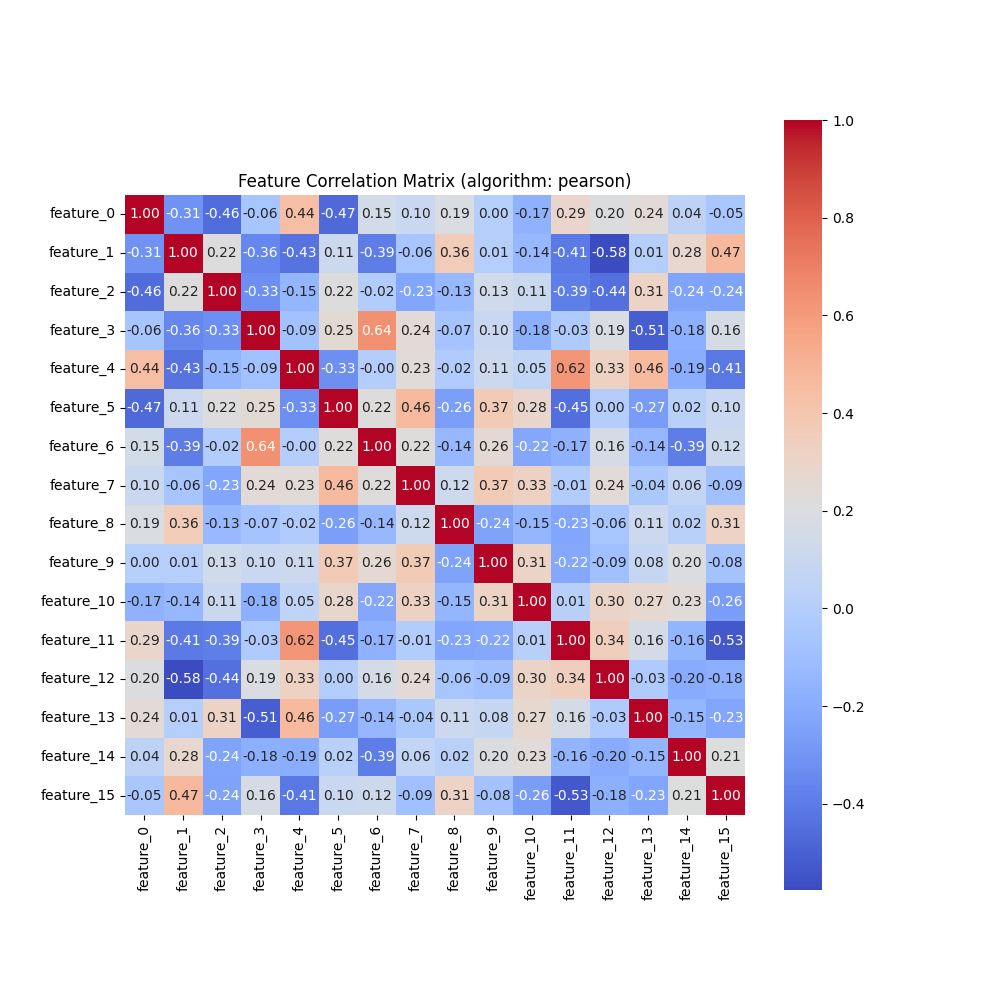
\includegraphics[width=0.8\linewidth]{img/annexes/26_filtered_chunk_extraction_-e_only-max-entropy_-s_none/Word2vec 5_correlation_matrix.png}} \\
\hline
\end{longtable}


\begin{longtable}{|c|c|}
\caption{Word2vec 6 Feature Engineering Results on 26\_filtered\_chunk\_extraction\_-e\_only-max-entropy\_-s\_none} \label{tab:26_filtered_chunk_extraction_-e_only-max-entropy_-s_none_word2vec_6_feature_engineering_results}\\
\hline
Dataset Name & 26\_filtered\_chunk\_extraction\_-e\_only-max-entropy\_-s\_none \\ \hline
Instance & Word2vec 6 \\ \hline
\multirow{8}{*}{Best Features} & feature\_13 \\ \cline{2-2}
 & feature\_1 \\ \cline{2-2}
 & feature\_5 \\ \cline{2-2}
 & feature\_2 \\ \cline{2-2}
 & feature\_3 \\ \cline{2-2}
 & feature\_9 \\ \cline{2-2}
 & feature\_6 \\ \cline{2-2}
 & feature\_4 \\ \cline{2-2}
\noalign{\vskip 5mm}
\multicolumn{2}{|c|}{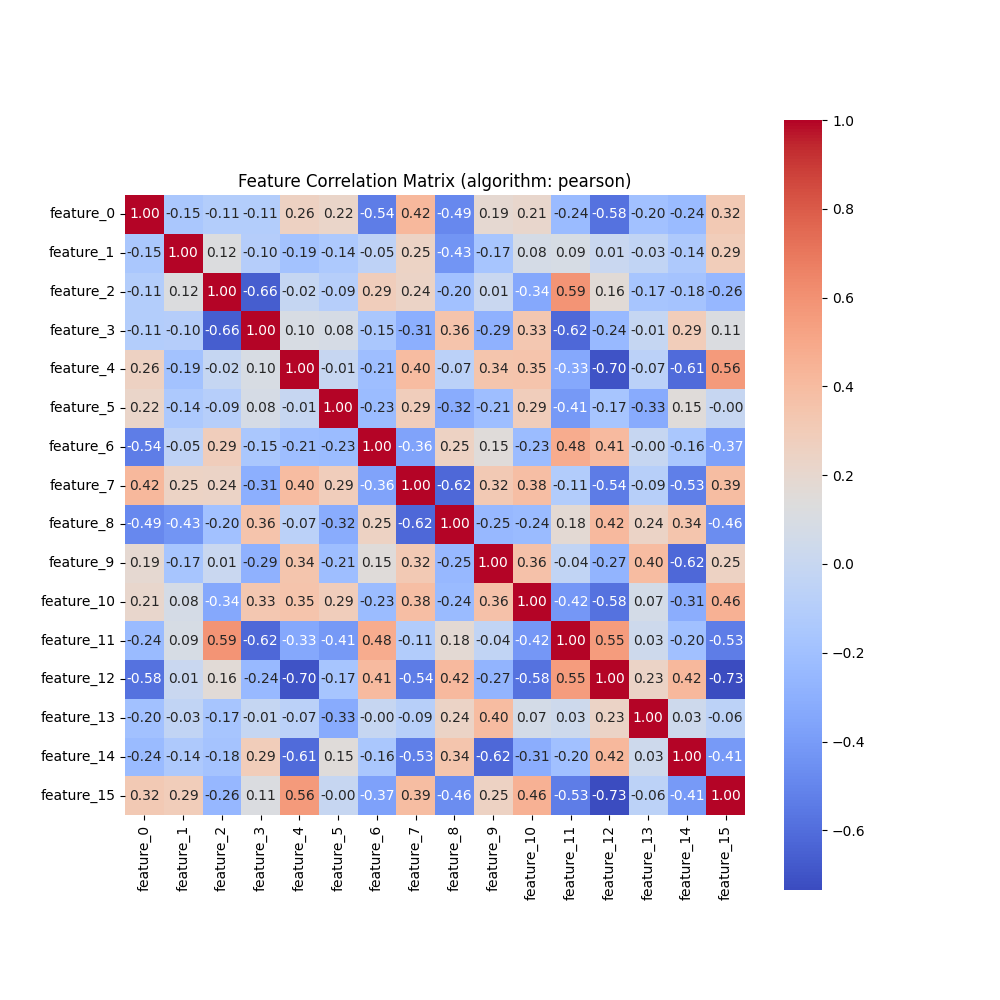
\includegraphics[width=0.8\linewidth]{img/annexes/26_filtered_chunk_extraction_-e_only-max-entropy_-s_none/Word2vec 6_correlation_matrix.png}} \\
\hline
\end{longtable}


\begin{longtable}{|c|c|}
\caption{Word2vec 7 Feature Engineering Results on 26\_filtered\_chunk\_extraction\_-e\_only-max-entropy\_-s\_none} \label{tab:26_filtered_chunk_extraction_-e_only-max-entropy_-s_none_word2vec_7_feature_engineering_results}\\
\hline
Dataset Name & 26\_filtered\_chunk\_extraction\_-e\_only-max-entropy\_-s\_none \\ \hline
Instance & Word2vec 7 \\ \hline
\multirow{8}{*}{Best Features} & feature\_4 \\ \cline{2-2}
 & feature\_3 \\ \cline{2-2}
 & feature\_12 \\ \cline{2-2}
 & feature\_10 \\ \cline{2-2}
 & feature\_15 \\ \cline{2-2}
 & feature\_0 \\ \cline{2-2}
 & feature\_7 \\ \cline{2-2}
 & feature\_9 \\ \cline{2-2}
\noalign{\vskip 5mm}
\multicolumn{2}{|c|}{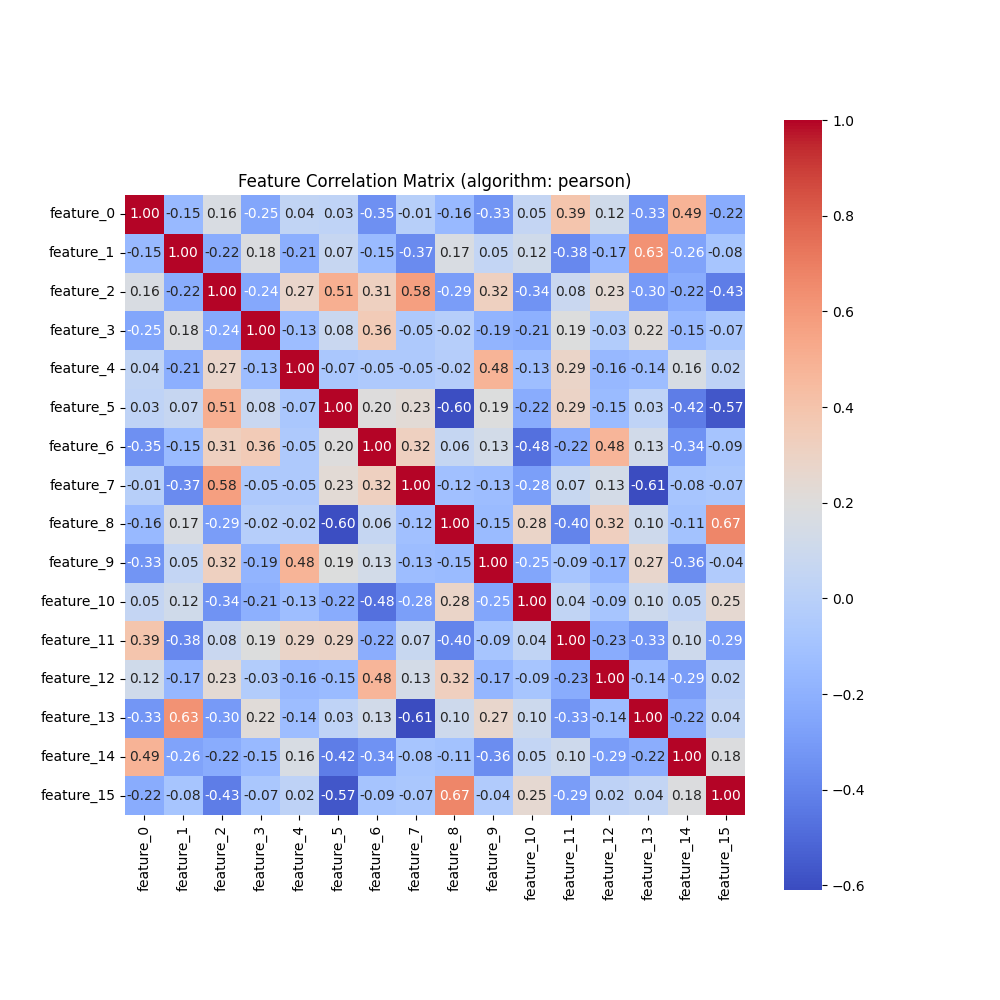
\includegraphics[width=0.8\linewidth]{img/annexes/26_filtered_chunk_extraction_-e_only-max-entropy_-s_none/Word2vec 7_correlation_matrix.png}} \\
\hline
\end{longtable}


\begin{longtable}{|c|c|}
\caption{Word2vec 8 Feature Engineering Results on 26\_filtered\_chunk\_extraction\_-e\_only-max-entropy\_-s\_none} \label{tab:26_filtered_chunk_extraction_-e_only-max-entropy_-s_none_word2vec_8_feature_engineering_results}\\
\hline
Dataset Name & 26\_filtered\_chunk\_extraction\_-e\_only-max-entropy\_-s\_none \\ \hline
Instance & Word2vec 8 \\ \hline
\multirow{8}{*}{Best Features} & feature\_60 \\ \cline{2-2}
 & feature\_80 \\ \cline{2-2}
 & feature\_55 \\ \cline{2-2}
 & feature\_85 \\ \cline{2-2}
 & feature\_16 \\ \cline{2-2}
 & feature\_75 \\ \cline{2-2}
 & feature\_31 \\ \cline{2-2}
 & feature\_51 \\ \cline{2-2}
\noalign{\vskip 5mm}
\multicolumn{2}{|c|}{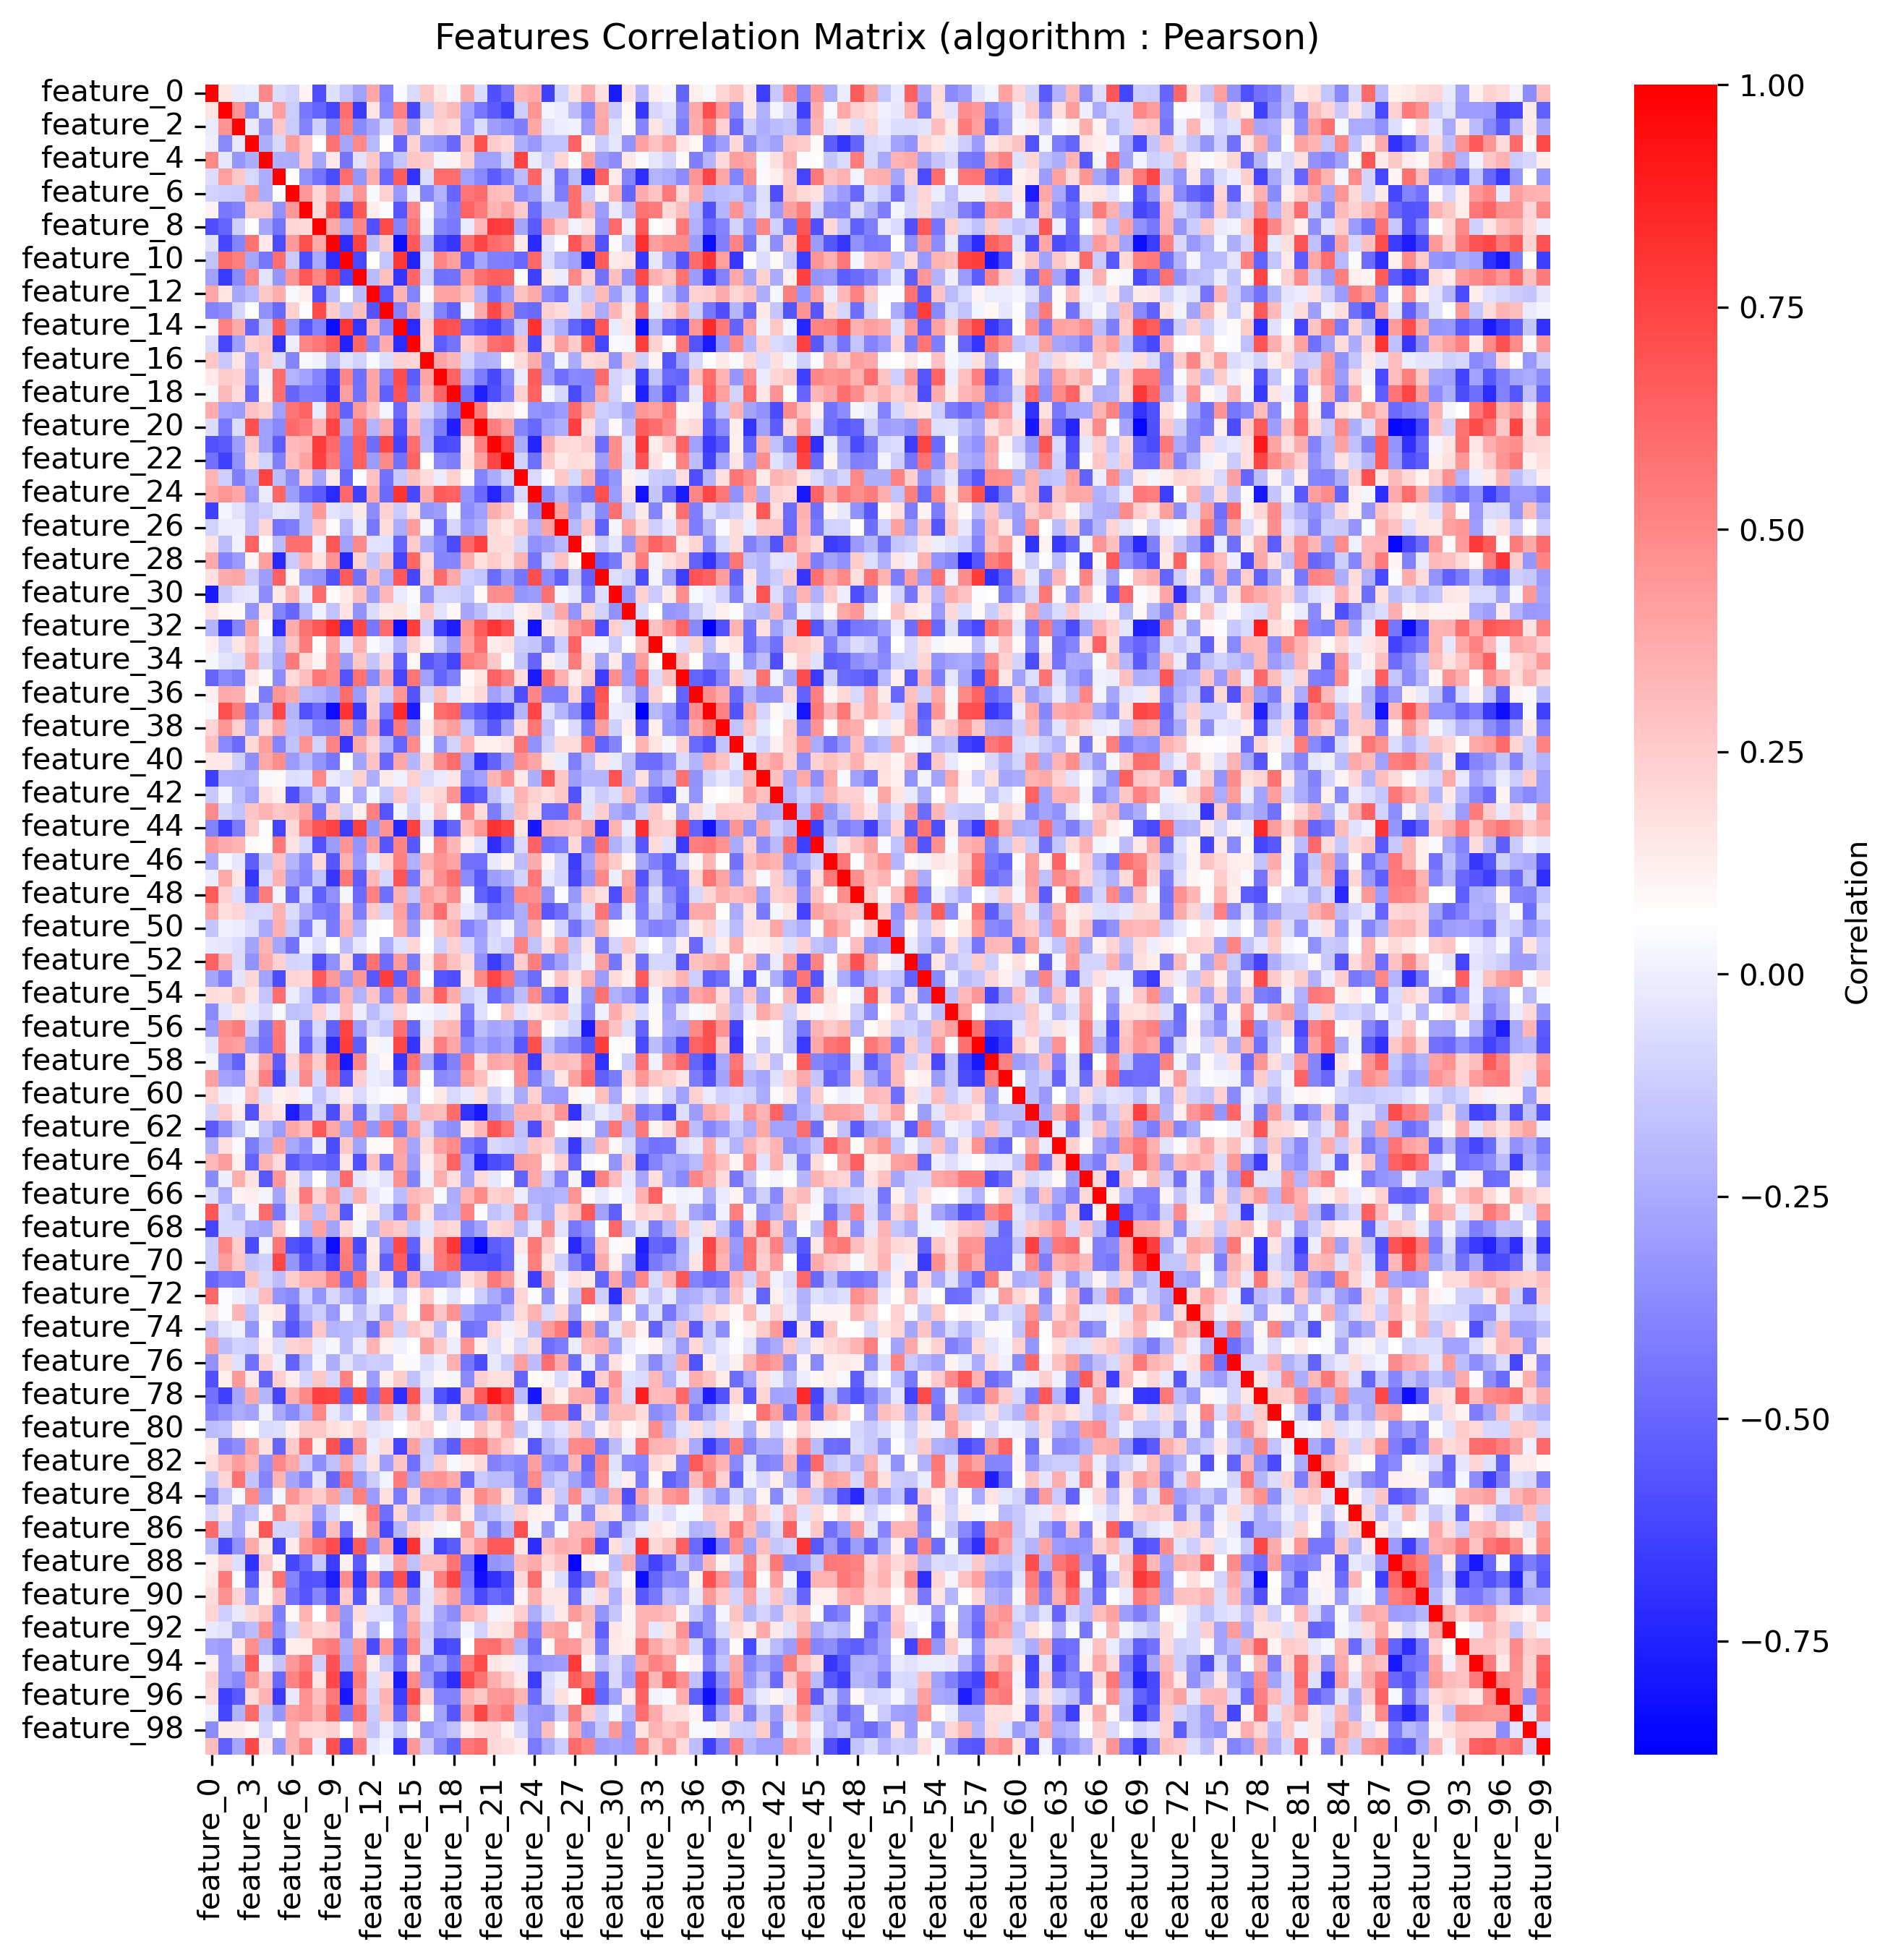
\includegraphics[width=0.8\linewidth]{img/annexes/26_filtered_chunk_extraction_-e_only-max-entropy_-s_none/Word2vec 8_correlation_matrix.png}} \\
\hline
\end{longtable}


\begin{longtable}{|c|c|}
\caption{Word2vec 9 Feature Engineering Results on 26\_filtered\_chunk\_extraction\_-e\_only-max-entropy\_-s\_none} \label{tab:26_filtered_chunk_extraction_-e_only-max-entropy_-s_none_word2vec_9_feature_engineering_results}\\
\hline
Dataset Name & 26\_filtered\_chunk\_extraction\_-e\_only-max-entropy\_-s\_none \\ \hline
Instance & Word2vec 9 \\ \hline
\multirow{8}{*}{Best Features} & feature\_34 \\ \cline{2-2}
 & feature\_40 \\ \cline{2-2}
 & feature\_19 \\ \cline{2-2}
 & feature\_30 \\ \cline{2-2}
 & feature\_28 \\ \cline{2-2}
 & feature\_62 \\ \cline{2-2}
 & feature\_35 \\ \cline{2-2}
 & feature\_91 \\ \cline{2-2}
\noalign{\vskip 5mm}
\multicolumn{2}{|c|}{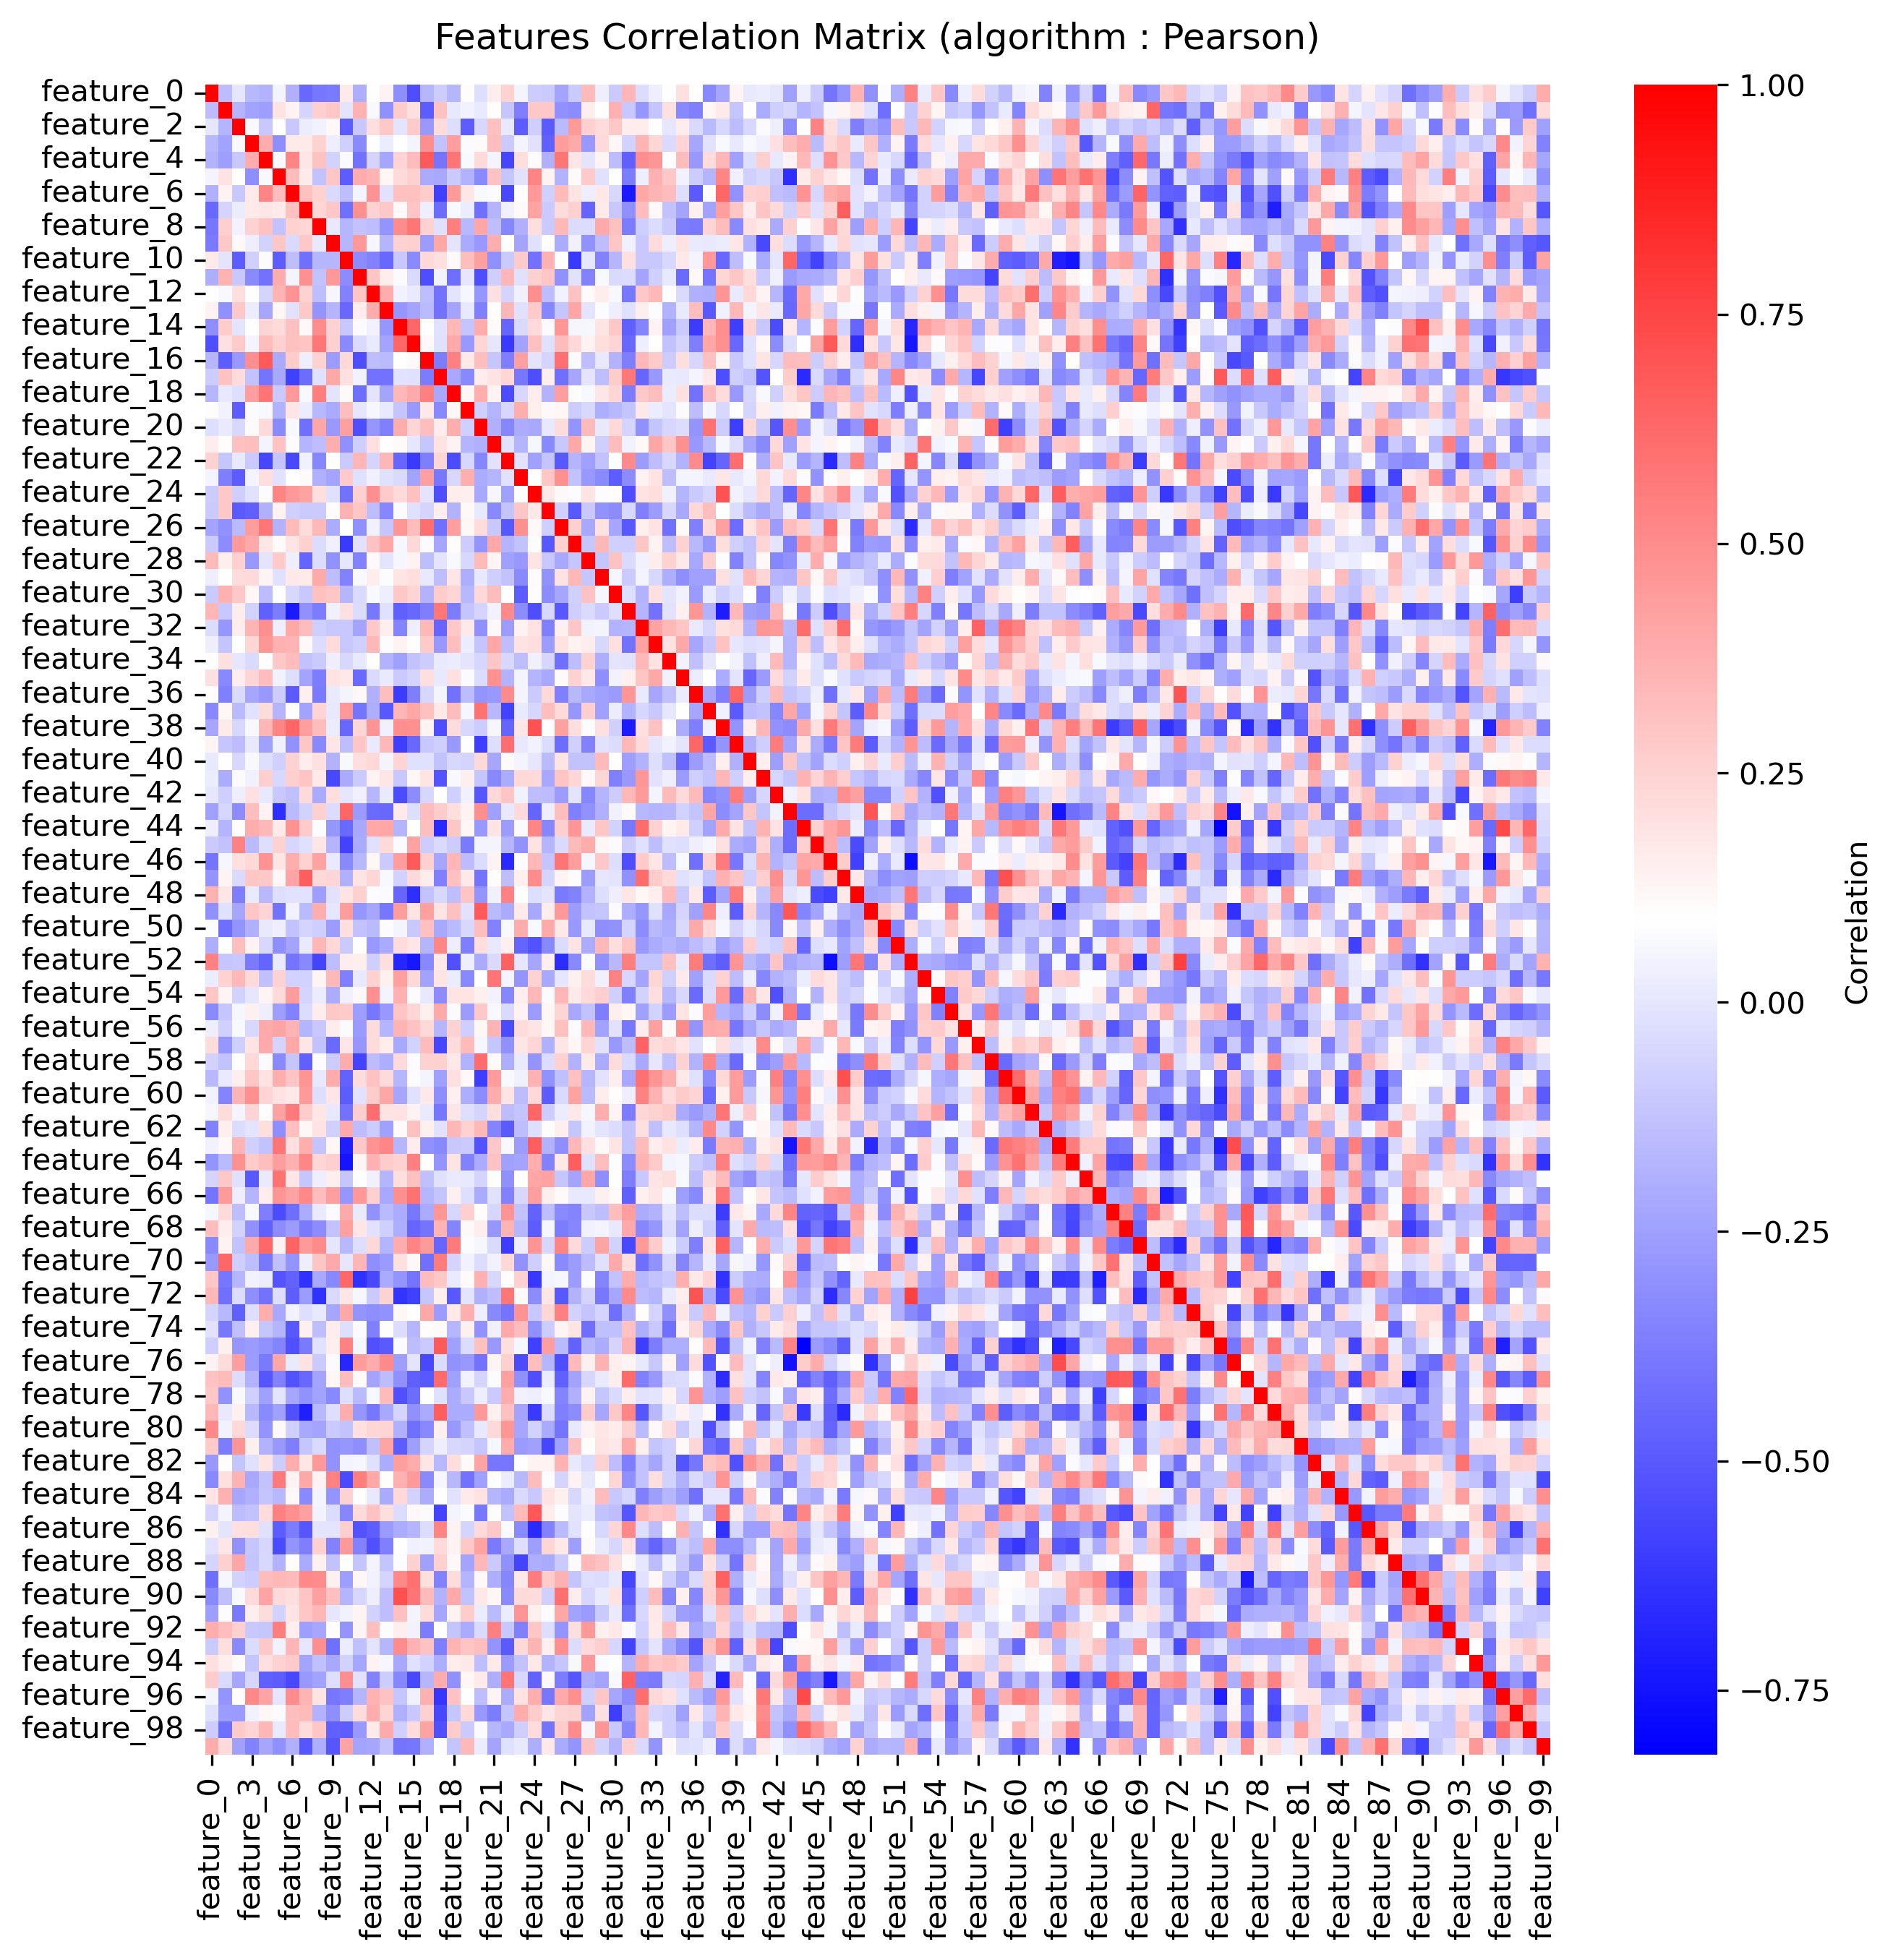
\includegraphics[width=0.8\linewidth]{img/annexes/26_filtered_chunk_extraction_-e_only-max-entropy_-s_none/Word2vec 9_correlation_matrix.png}} \\
\hline
\end{longtable}


\begin{longtable}{|c|c|}
\caption{Word2vec 10 Feature Engineering Results on 26\_filtered\_chunk\_extraction\_-e\_only-max-entropy\_-s\_none} \label{tab:26_filtered_chunk_extraction_-e_only-max-entropy_-s_none_word2vec_10_feature_engineering_results}\\
\hline
Dataset Name & 26\_filtered\_chunk\_extraction\_-e\_only-max-entropy\_-s\_none \\ \hline
Instance & Word2vec 10 \\ \hline
\multirow{8}{*}{Best Features} & feature\_24 \\ \cline{2-2}
 & feature\_4 \\ \cline{2-2}
 & feature\_85 \\ \cline{2-2}
 & feature\_46 \\ \cline{2-2}
 & feature\_71 \\ \cline{2-2}
 & feature\_76 \\ \cline{2-2}
 & feature\_42 \\ \cline{2-2}
 & feature\_19 \\ \cline{2-2}
\noalign{\vskip 5mm}
\multicolumn{2}{|c|}{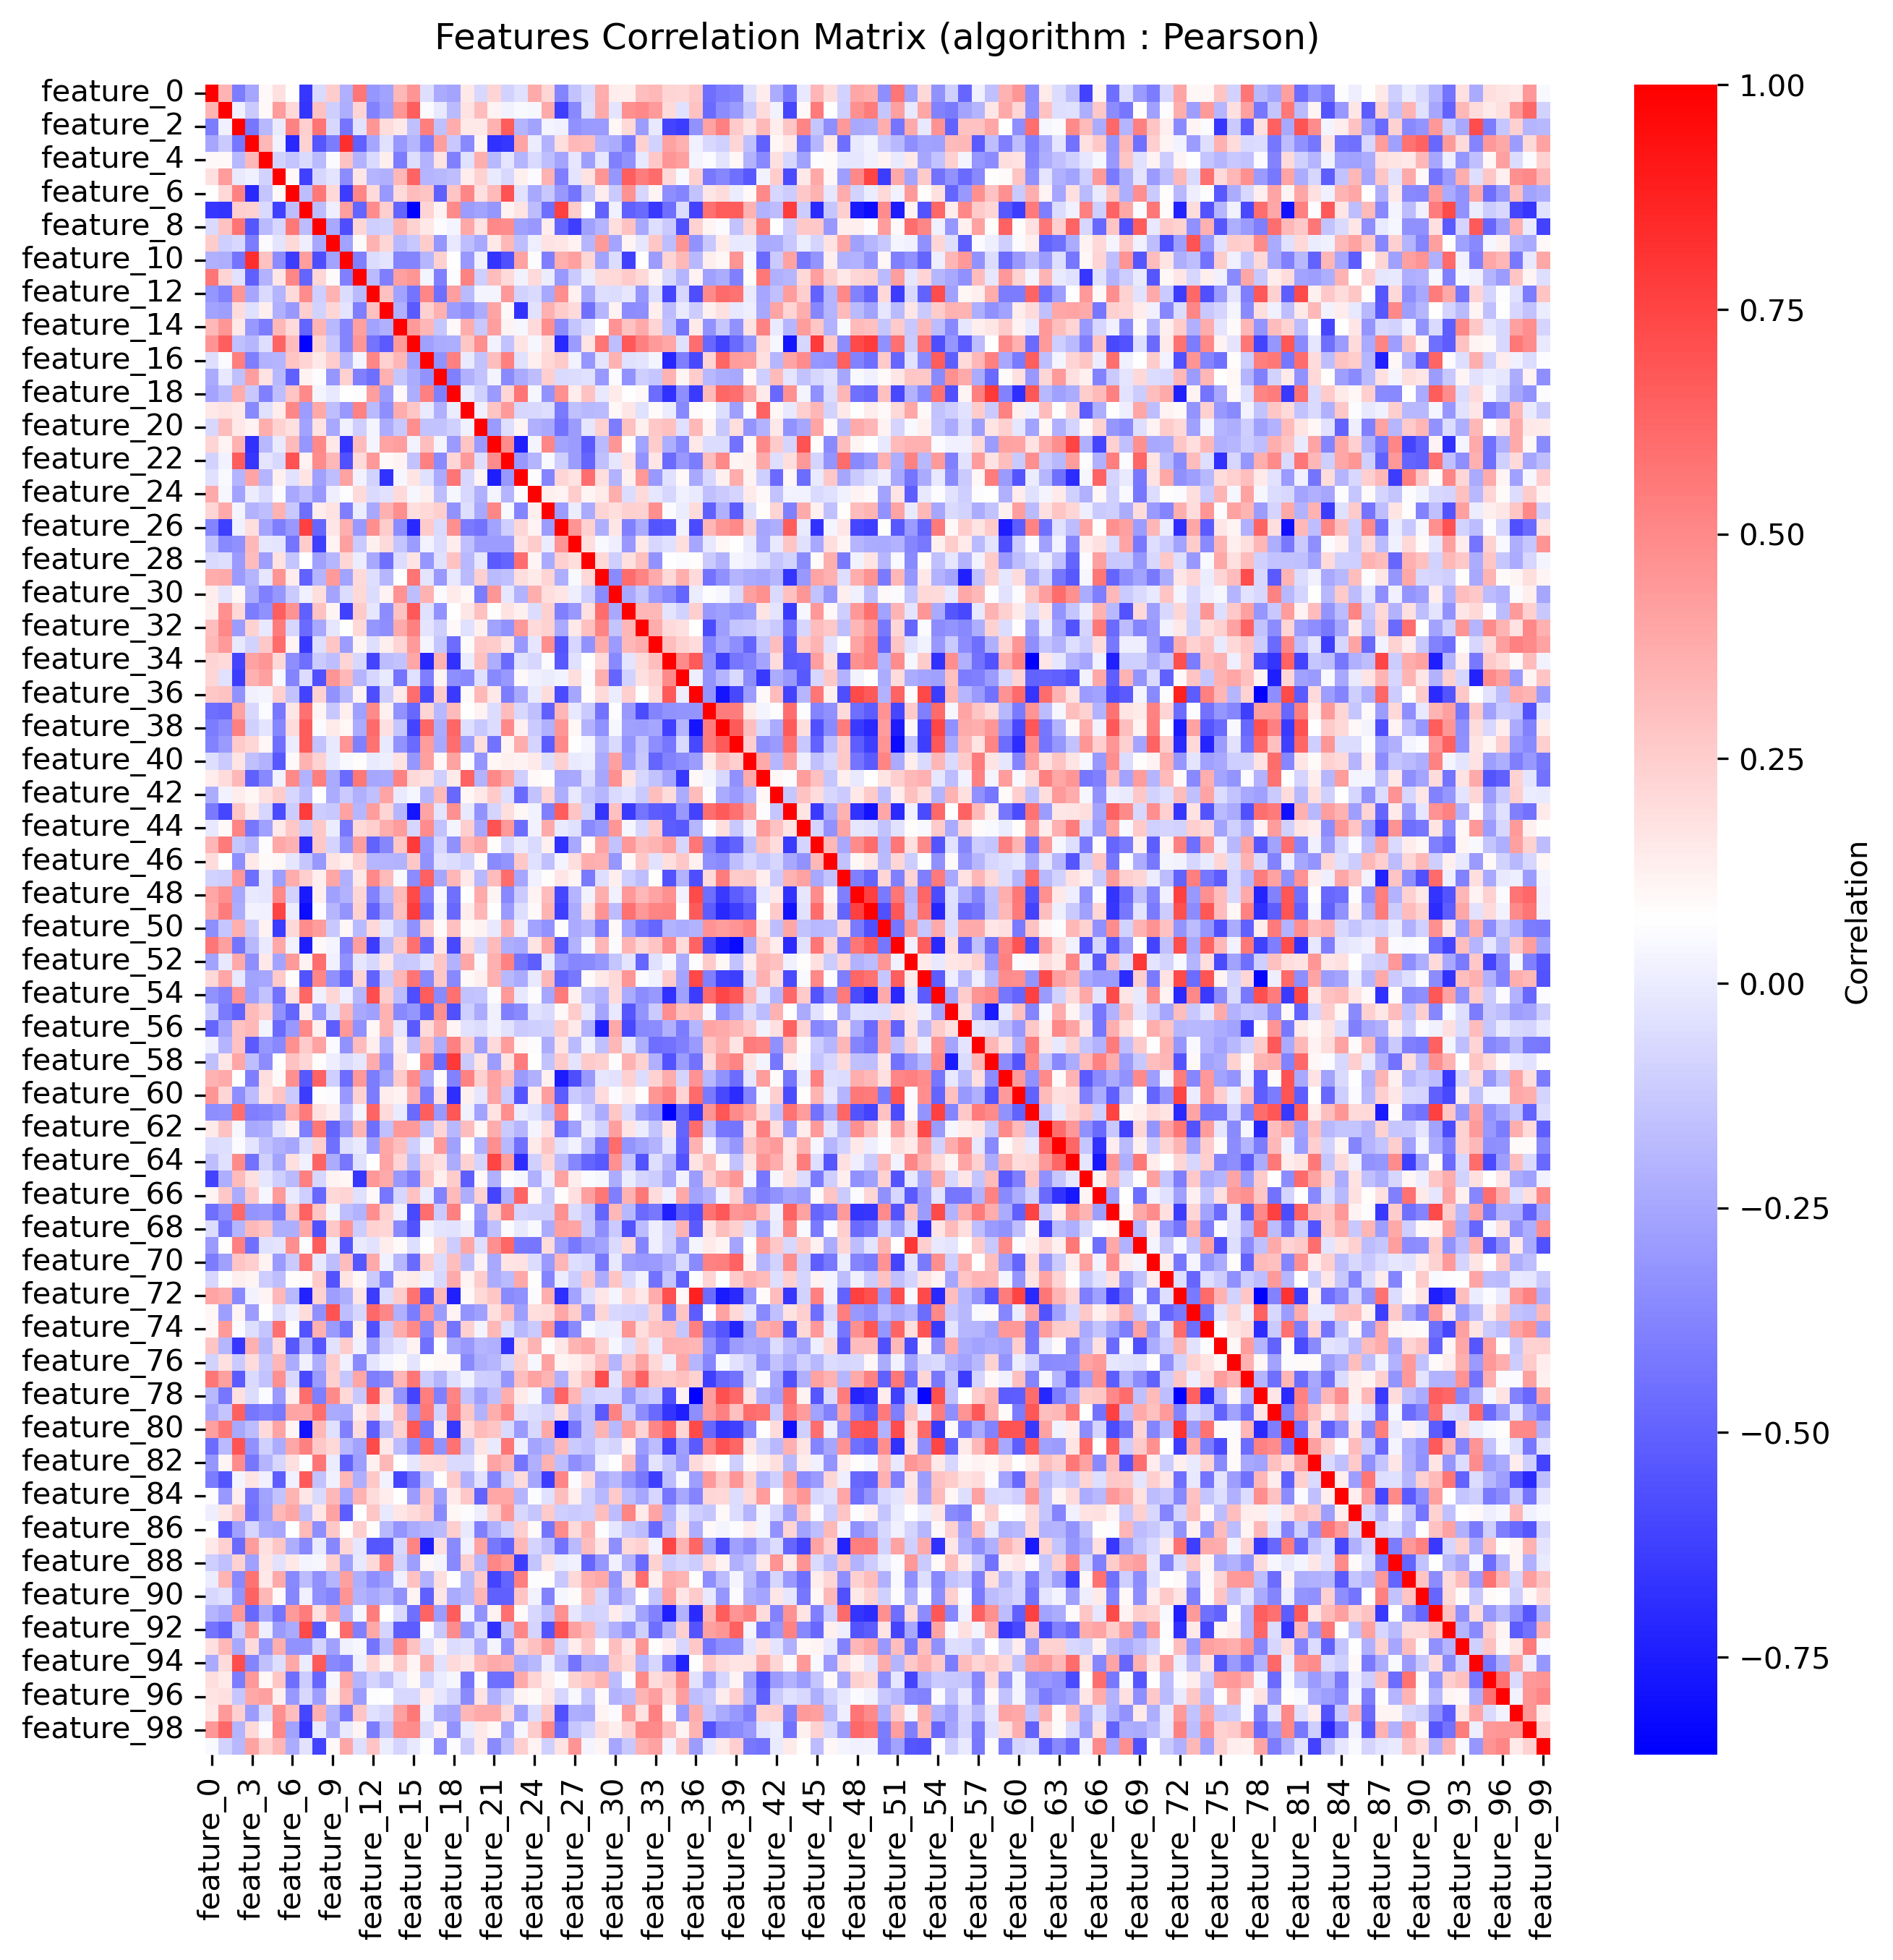
\includegraphics[width=0.8\linewidth]{img/annexes/26_filtered_chunk_extraction_-e_only-max-entropy_-s_none/Word2vec 10_correlation_matrix.png}} \\
\hline
\end{longtable}


\begin{longtable}{|c|c|}
\caption{Word2vec 11 Feature Engineering Results on 26\_filtered\_chunk\_extraction\_-e\_only-max-entropy\_-s\_none} \label{tab:26_filtered_chunk_extraction_-e_only-max-entropy_-s_none_word2vec_11_feature_engineering_results}\\
\hline
Dataset Name & 26\_filtered\_chunk\_extraction\_-e\_only-max-entropy\_-s\_none \\ \hline
Instance & Word2vec 11 \\ \hline
\multirow{8}{*}{Best Features} & feature\_41 \\ \cline{2-2}
 & feature\_85 \\ \cline{2-2}
 & feature\_22 \\ \cline{2-2}
 & feature\_79 \\ \cline{2-2}
 & feature\_70 \\ \cline{2-2}
 & feature\_18 \\ \cline{2-2}
 & feature\_64 \\ \cline{2-2}
 & feature\_91 \\ \cline{2-2}
\noalign{\vskip 5mm}
\multicolumn{2}{|c|}{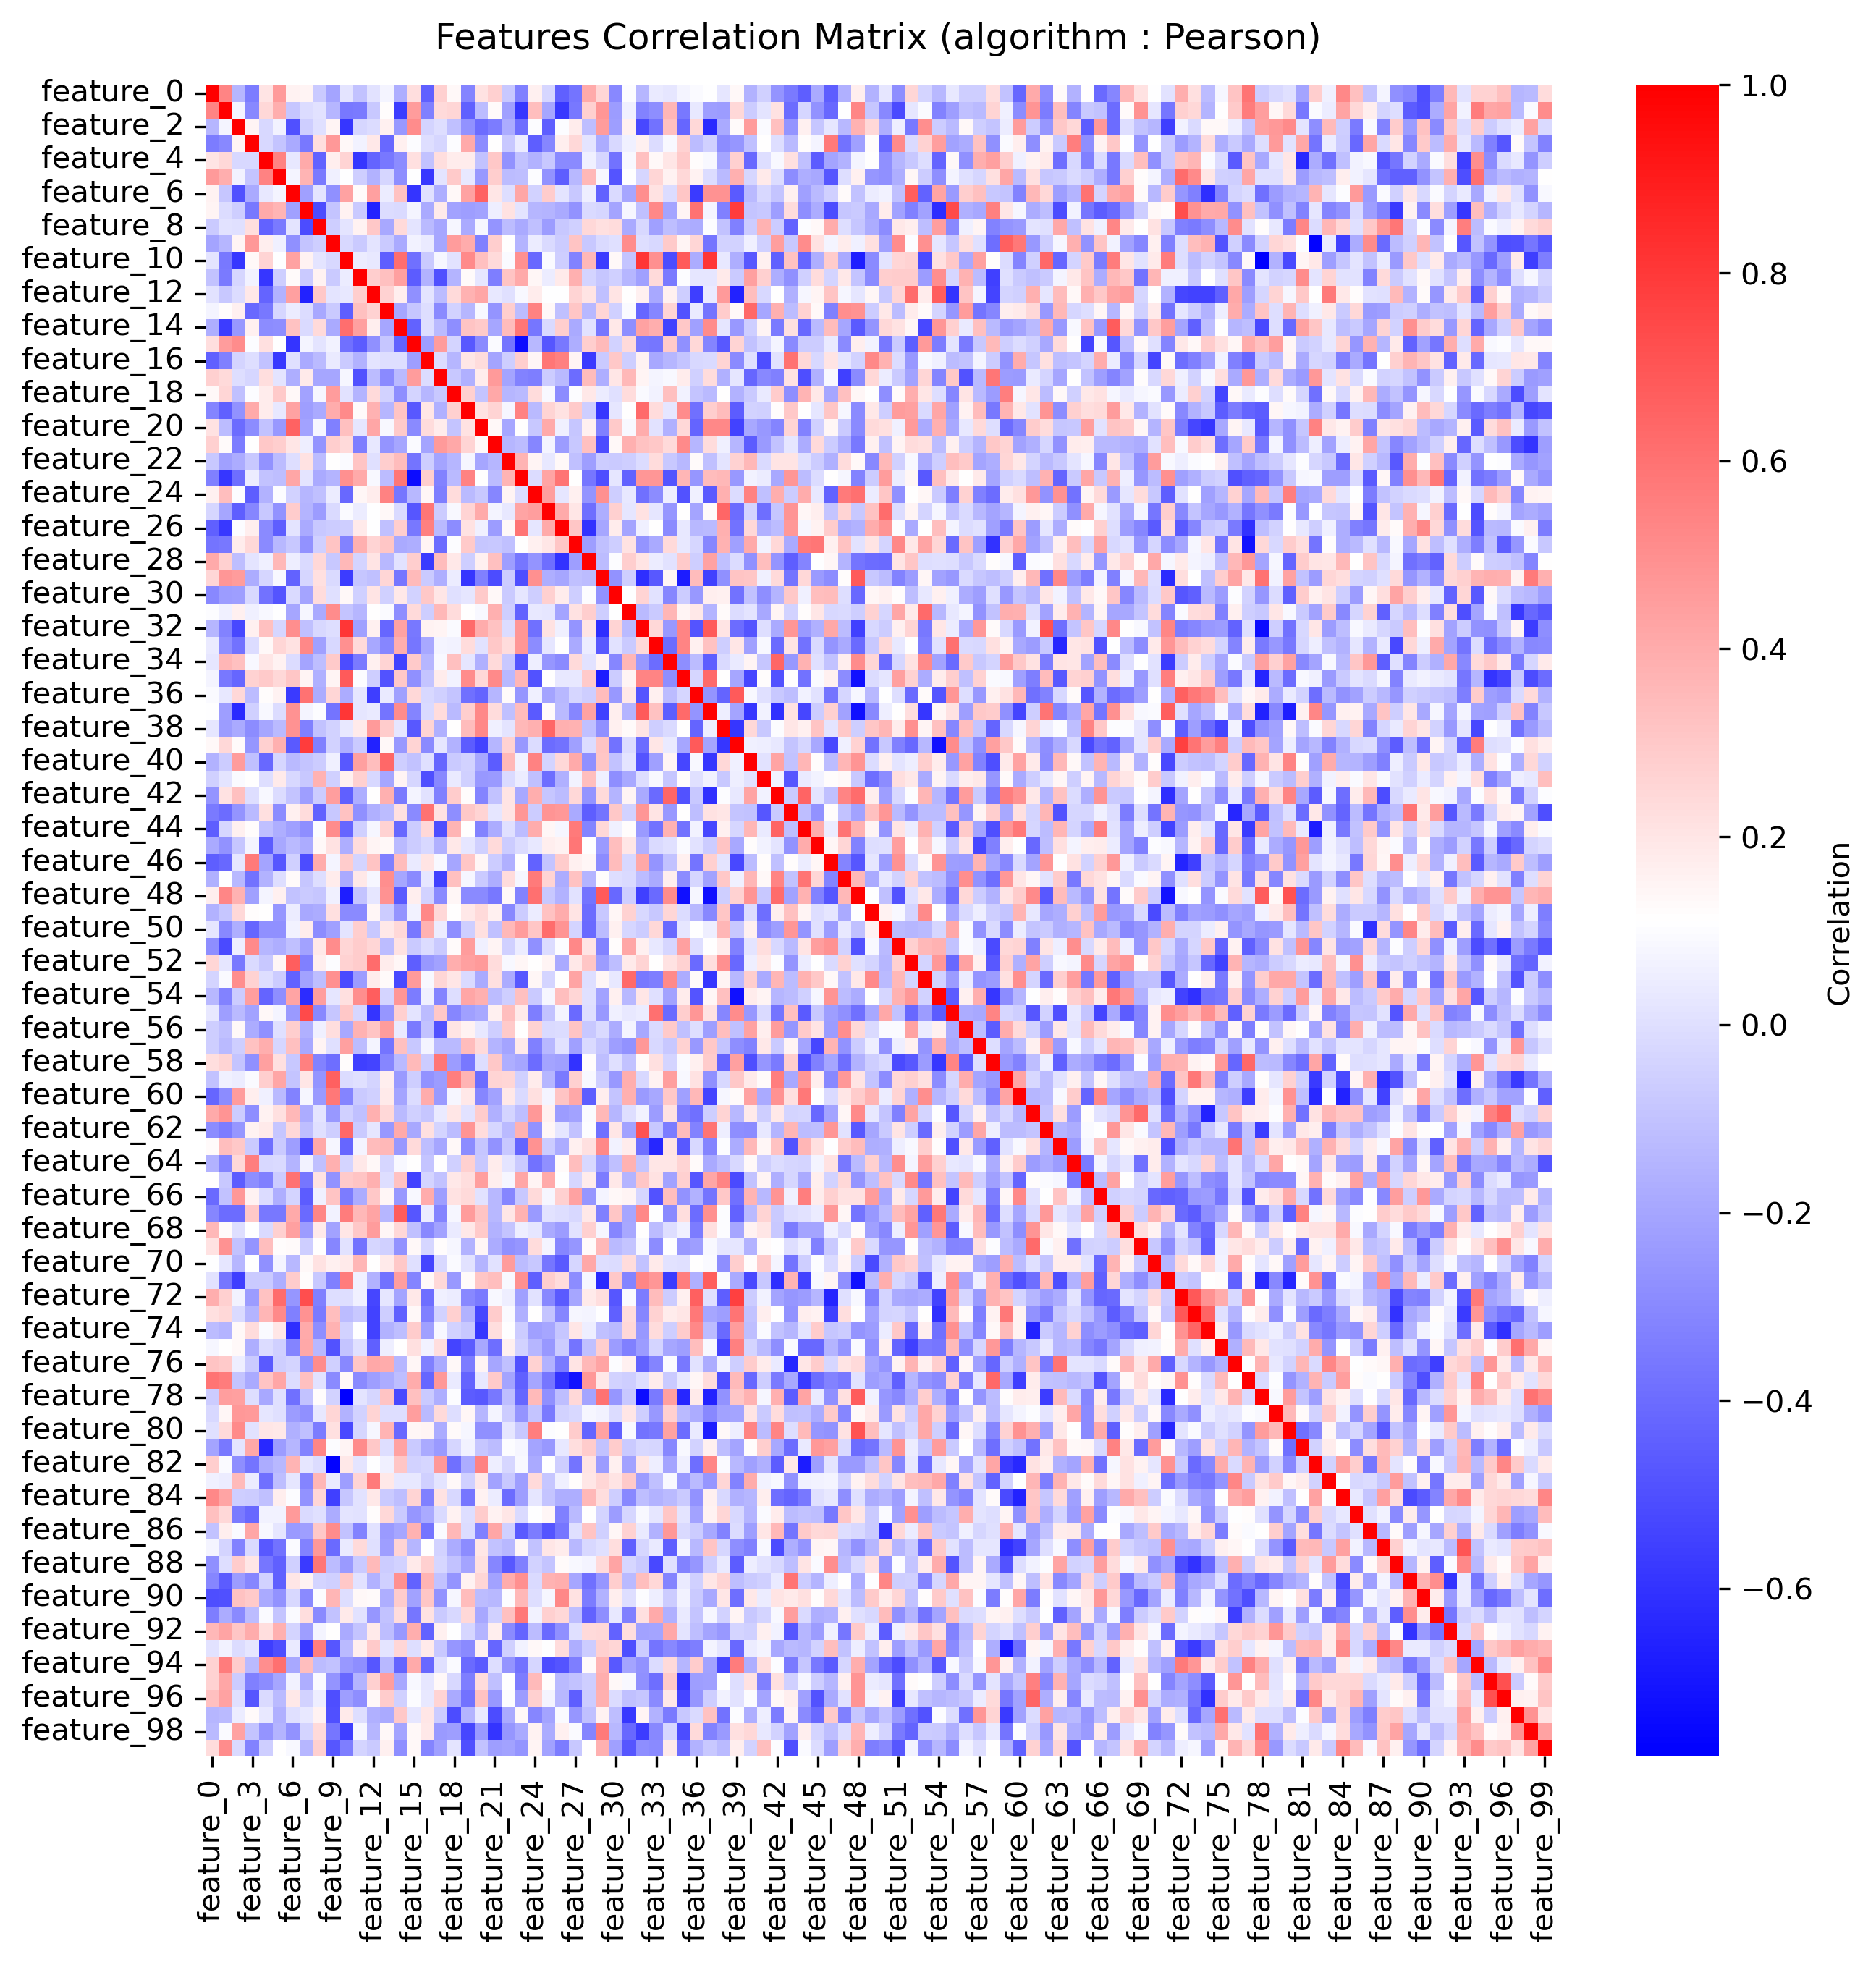
\includegraphics[width=0.8\linewidth]{img/annexes/26_filtered_chunk_extraction_-e_only-max-entropy_-s_none/Word2vec 11_correlation_matrix.png}} \\
\hline
\end{longtable}


\subsection{27\_filtered\_chunk\_extraction\_-e\_only-max-entropy\_-s\_activate}

\begin{longtable}{|c|c|}
\caption{Transformers 0 Feature Engineering Results on 27\_filtered\_chunk\_extraction\_-e\_only-max-entropy\_-s\_activate} \label{tab:27_filtered_chunk_extraction_-e_only-max-entropy_-s_activate_transformers_0_feature_engineering_results}\\
\hline
Dataset Name & 27\_filtered\_chunk\_extraction\_-e\_only-max-entropy\_-s\_activate \\ \hline
Instance & Transformers 0 \\ \hline
\multirow{8}{*}{Best Features} & embedded\_0 \\ \cline{2-2}
 & embedded\_1 \\ \cline{2-2}
 & embedded\_4 \\ \cline{2-2}
 & embedded\_5 \\ \cline{2-2}
 & embedded\_7 \\ \cline{2-2}
 & embedded\_6 \\ \cline{2-2}
 & embedded\_3 \\ \cline{2-2}
 & embedded\_2 \\ \cline{2-2}
\noalign{\vskip 5mm}
\multicolumn{2}{|c|}{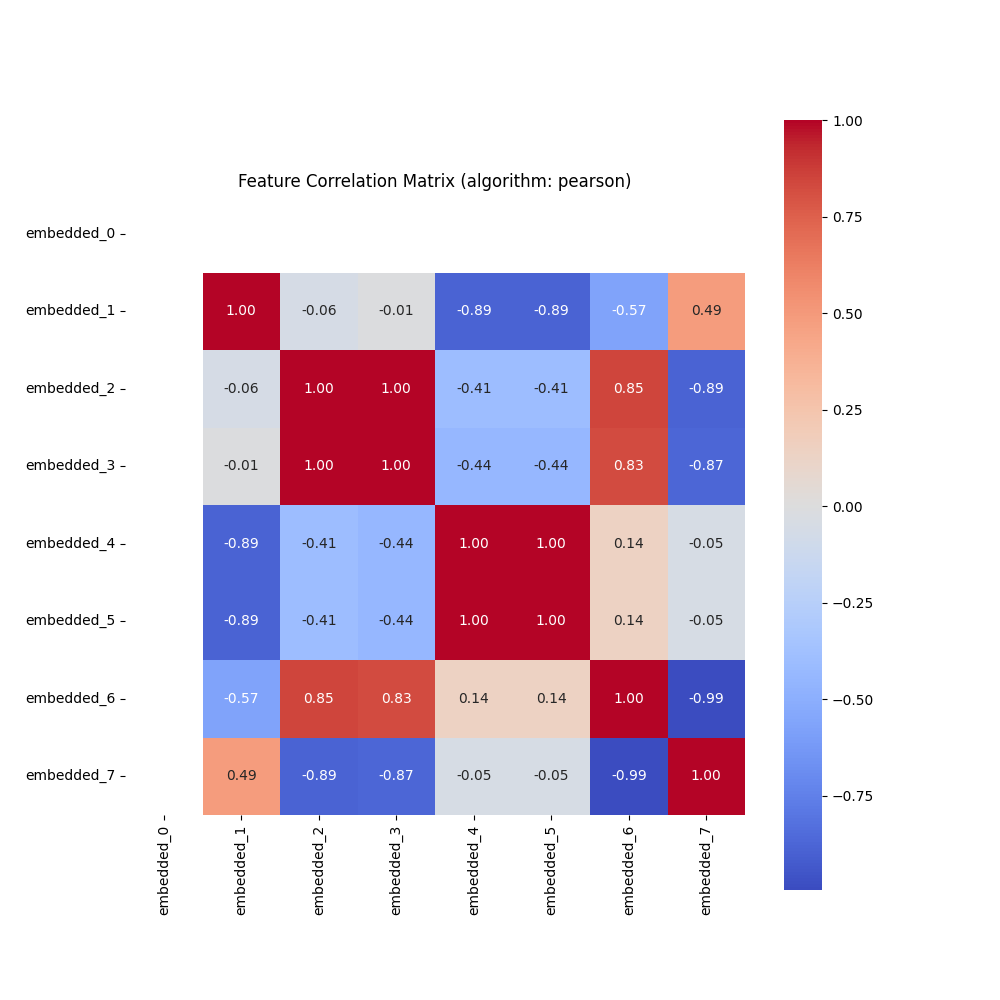
\includegraphics[width=0.8\linewidth]{img/annexes/27_filtered_chunk_extraction_-e_only-max-entropy_-s_activate/Transformers 0_correlation_matrix.png}} \\
\hline
\end{longtable}


\begin{longtable}{|c|c|}
\caption{Transformers 1 Feature Engineering Results on 27\_filtered\_chunk\_extraction\_-e\_only-max-entropy\_-s\_activate} \label{tab:27_filtered_chunk_extraction_-e_only-max-entropy_-s_activate_transformers_1_feature_engineering_results}\\
\hline
Dataset Name & 27\_filtered\_chunk\_extraction\_-e\_only-max-entropy\_-s\_activate \\ \hline
Instance & Transformers 1 \\ \hline
\multirow{8}{*}{Best Features} & embedded\_0 \\ \cline{2-2}
 & embedded\_6 \\ \cline{2-2}
 & embedded\_7 \\ \cline{2-2}
 & embedded\_9 \\ \cline{2-2}
 & embedded\_8 \\ \cline{2-2}
 & embedded\_10 \\ \cline{2-2}
 & embedded\_5 \\ \cline{2-2}
 & embedded\_3 \\ \cline{2-2}
\noalign{\vskip 5mm}
\multicolumn{2}{|c|}{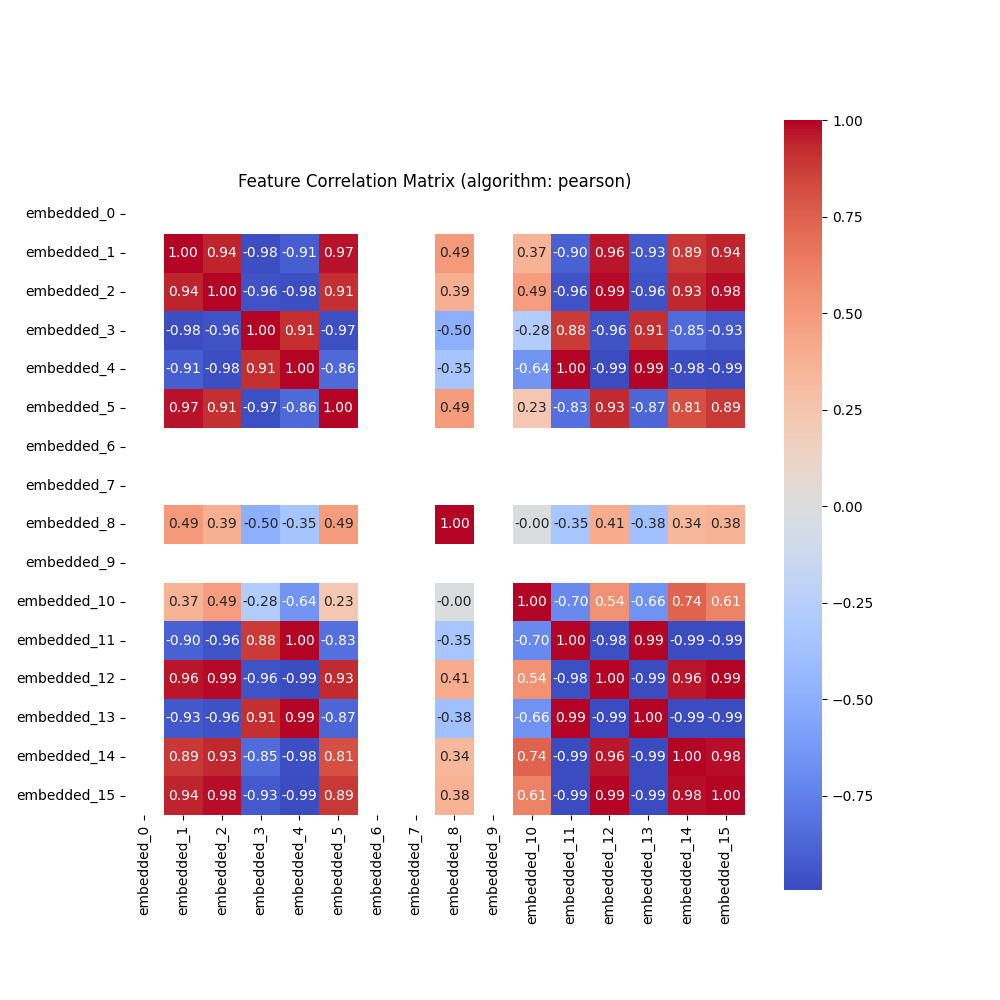
\includegraphics[width=0.8\linewidth]{img/annexes/27_filtered_chunk_extraction_-e_only-max-entropy_-s_activate/Transformers 1_correlation_matrix.png}} \\
\hline
\end{longtable}


\begin{longtable}{|c|c|}
\caption{Transformers 2 Feature Engineering Results on 27\_filtered\_chunk\_extraction\_-e\_only-max-entropy\_-s\_activate} \label{tab:27_filtered_chunk_extraction_-e_only-max-entropy_-s_activate_transformers_2_feature_engineering_results}\\
\hline
Dataset Name & 27\_filtered\_chunk\_extraction\_-e\_only-max-entropy\_-s\_activate \\ \hline
Instance & Transformers 2 \\ \hline
\multirow{8}{*}{Best Features} & embedded\_0 \\ \cline{2-2}
 & embedded\_3 \\ \cline{2-2}
 & embedded\_7 \\ \cline{2-2}
 & embedded\_6 \\ \cline{2-2}
 & embedded\_1 \\ \cline{2-2}
 & embedded\_2 \\ \cline{2-2}
 & embedded\_5 \\ \cline{2-2}
 & embedded\_4 \\ \cline{2-2}
\noalign{\vskip 5mm}
\multicolumn{2}{|c|}{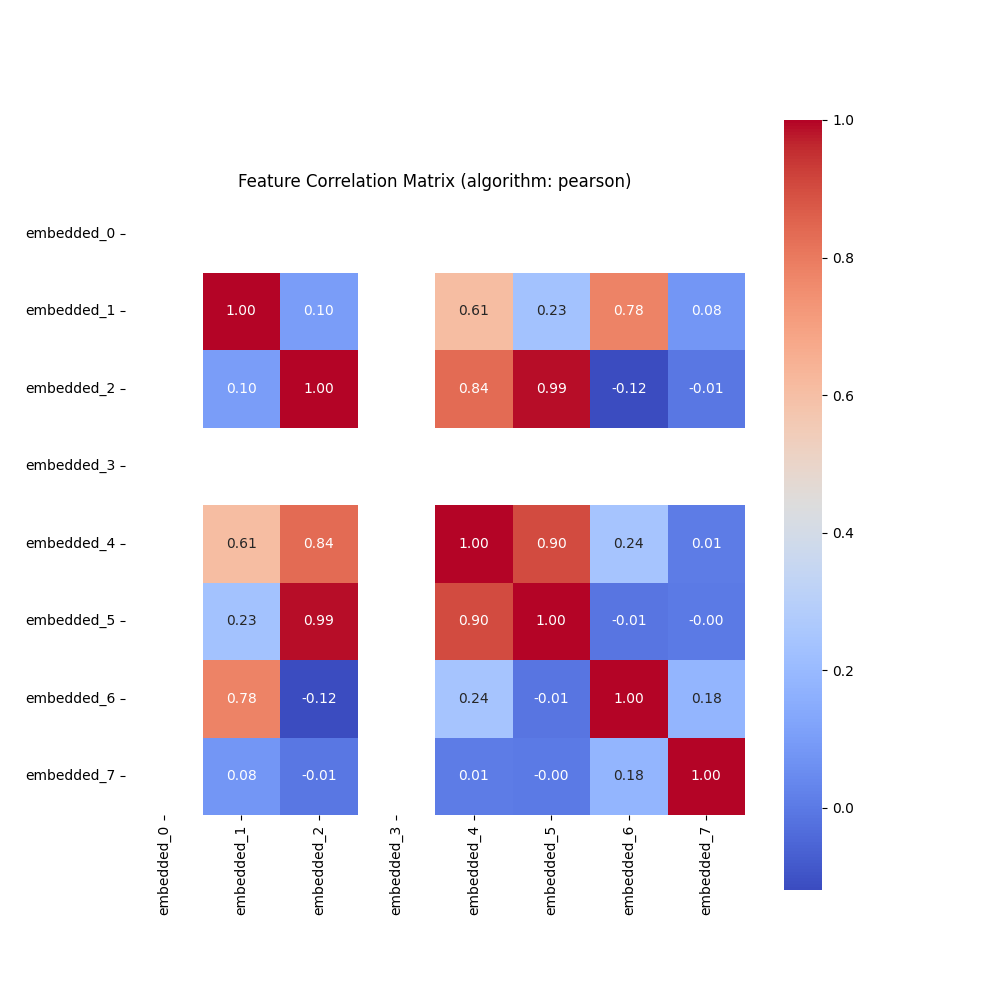
\includegraphics[width=0.8\linewidth]{img/annexes/27_filtered_chunk_extraction_-e_only-max-entropy_-s_activate/Transformers 2_correlation_matrix.png}} \\
\hline
\end{longtable}


\begin{longtable}{|c|c|}
\caption{Transformers 3 Feature Engineering Results on 27\_filtered\_chunk\_extraction\_-e\_only-max-entropy\_-s\_activate} \label{tab:27_filtered_chunk_extraction_-e_only-max-entropy_-s_activate_transformers_3_feature_engineering_results}\\
\hline
Dataset Name & 27\_filtered\_chunk\_extraction\_-e\_only-max-entropy\_-s\_activate \\ \hline
Instance & Transformers 3 \\ \hline
\multirow{8}{*}{Best Features} & embedded\_0 \\ \cline{2-2}
 & embedded\_2 \\ \cline{2-2}
 & embedded\_3 \\ \cline{2-2}
 & embedded\_7 \\ \cline{2-2}
 & embedded\_14 \\ \cline{2-2}
 & embedded\_9 \\ \cline{2-2}
 & embedded\_13 \\ \cline{2-2}
 & embedded\_5 \\ \cline{2-2}
\noalign{\vskip 5mm}
\multicolumn{2}{|c|}{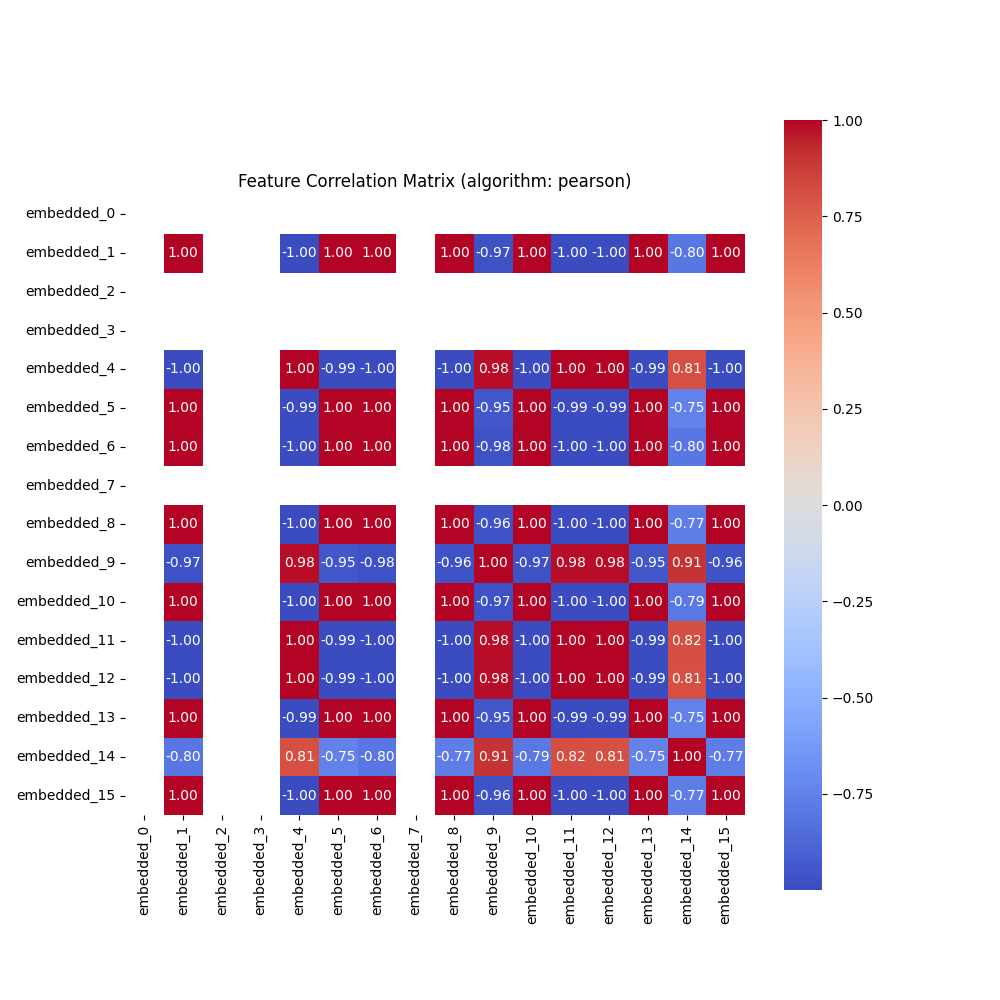
\includegraphics[width=0.8\linewidth]{img/annexes/27_filtered_chunk_extraction_-e_only-max-entropy_-s_activate/Transformers 3_correlation_matrix.png}} \\
\hline
\end{longtable}


\begin{longtable}{|c|c|}
\caption{Transformers 4 Feature Engineering Results on 27\_filtered\_chunk\_extraction\_-e\_only-max-entropy\_-s\_activate} \label{tab:27_filtered_chunk_extraction_-e_only-max-entropy_-s_activate_transformers_4_feature_engineering_results}\\
\hline
Dataset Name & 27\_filtered\_chunk\_extraction\_-e\_only-max-entropy\_-s\_activate \\ \hline
Instance & Transformers 4 \\ \hline
\multirow{8}{*}{Best Features} & embedded\_4 \\ \cline{2-2}
 & embedded\_1 \\ \cline{2-2}
 & embedded\_5 \\ \cline{2-2}
 & embedded\_7 \\ \cline{2-2}
 & embedded\_6 \\ \cline{2-2}
 & embedded\_3 \\ \cline{2-2}
 & embedded\_0 \\ \cline{2-2}
 & embedded\_2 \\ \cline{2-2}
\noalign{\vskip 5mm}
\multicolumn{2}{|c|}{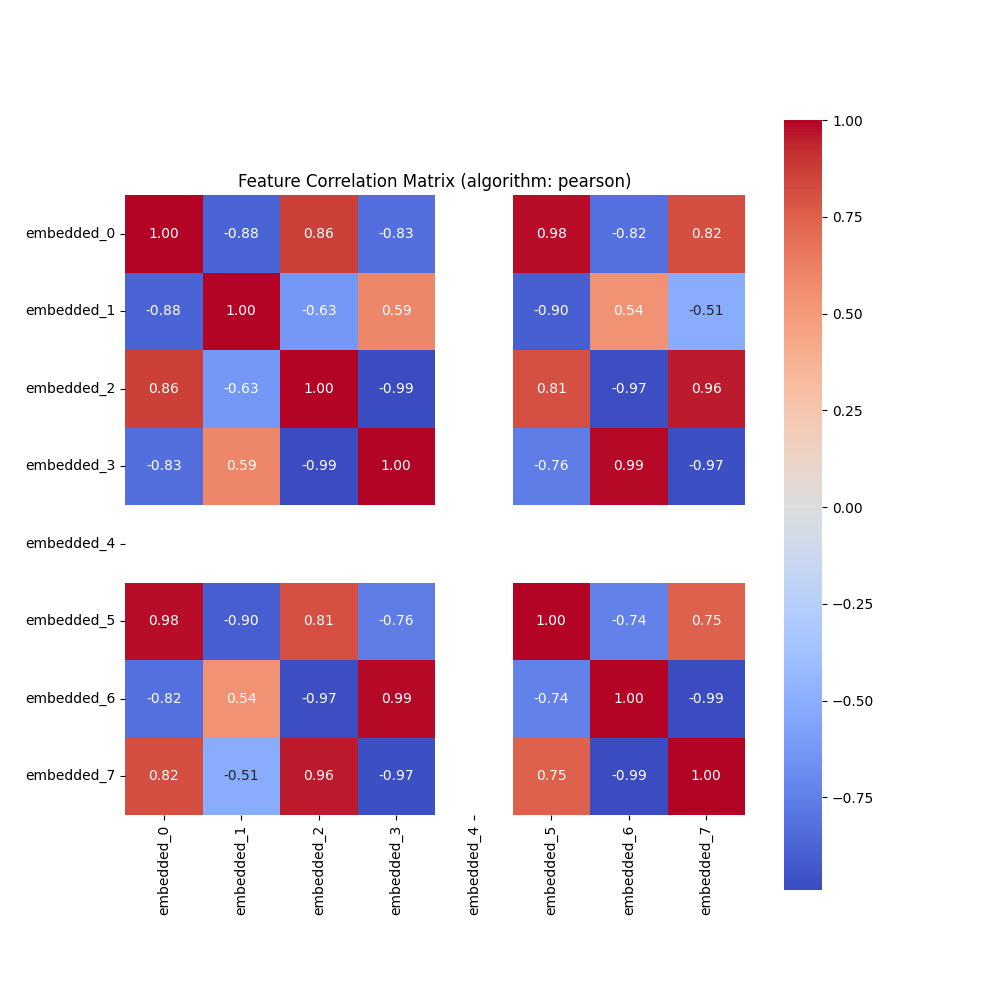
\includegraphics[width=0.8\linewidth]{img/annexes/27_filtered_chunk_extraction_-e_only-max-entropy_-s_activate/Transformers 4_correlation_matrix.png}} \\
\hline
\end{longtable}


\begin{longtable}{|c|c|}
\caption{Transformers 5 Feature Engineering Results on 27\_filtered\_chunk\_extraction\_-e\_only-max-entropy\_-s\_activate} \label{tab:27_filtered_chunk_extraction_-e_only-max-entropy_-s_activate_transformers_5_feature_engineering_results}\\
\hline
Dataset Name & 27\_filtered\_chunk\_extraction\_-e\_only-max-entropy\_-s\_activate \\ \hline
Instance & Transformers 5 \\ \hline
\multirow{8}{*}{Best Features} & embedded\_2 \\ \cline{2-2}
 & embedded\_4 \\ \cline{2-2}
 & embedded\_5 \\ \cline{2-2}
 & embedded\_6 \\ \cline{2-2}
 & embedded\_8 \\ \cline{2-2}
 & embedded\_14 \\ \cline{2-2}
 & embedded\_15 \\ \cline{2-2}
 & embedded\_0 \\ \cline{2-2}
\noalign{\vskip 5mm}
\multicolumn{2}{|c|}{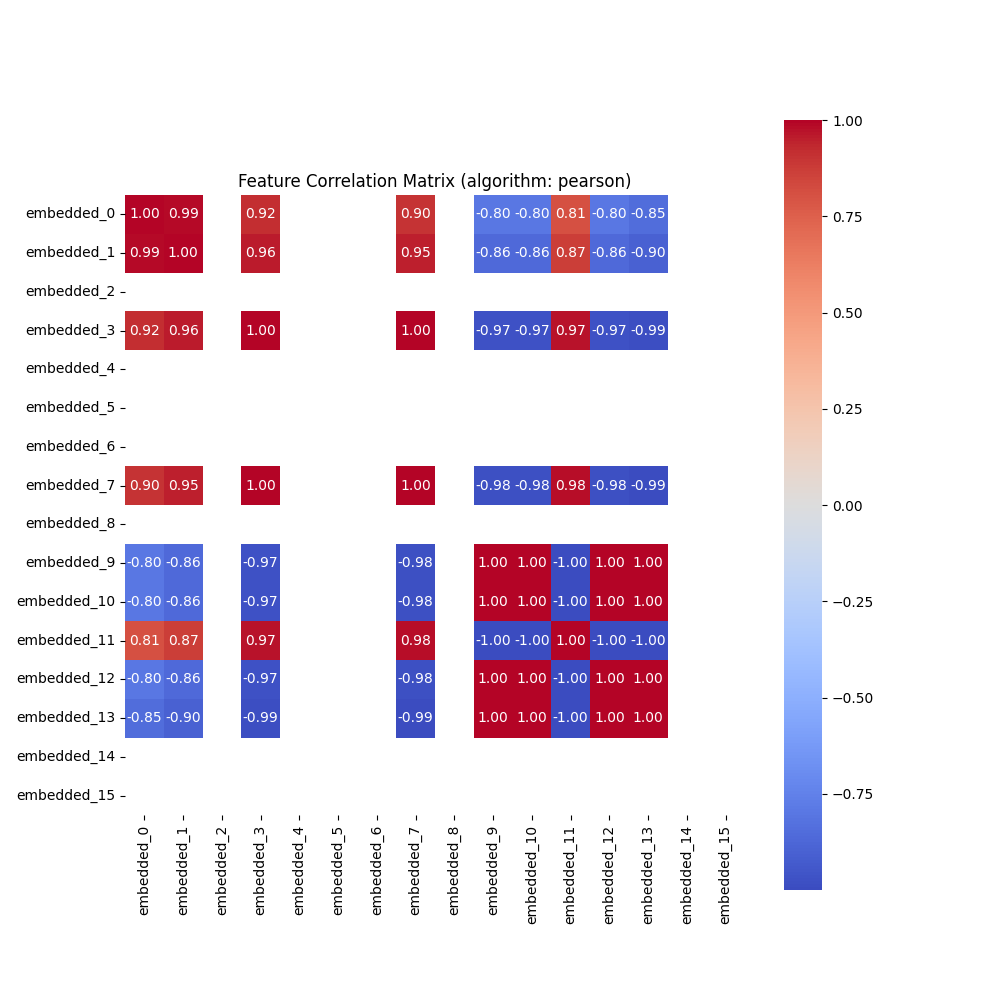
\includegraphics[width=0.8\linewidth]{img/annexes/27_filtered_chunk_extraction_-e_only-max-entropy_-s_activate/Transformers 5_correlation_matrix.png}} \\
\hline
\end{longtable}


\begin{longtable}{|c|c|}
\caption{Transformers 6 Feature Engineering Results on 27\_filtered\_chunk\_extraction\_-e\_only-max-entropy\_-s\_activate} \label{tab:27_filtered_chunk_extraction_-e_only-max-entropy_-s_activate_transformers_6_feature_engineering_results}\\
\hline
Dataset Name & 27\_filtered\_chunk\_extraction\_-e\_only-max-entropy\_-s\_activate \\ \hline
Instance & Transformers 6 \\ \hline
\multirow{8}{*}{Best Features} & embedded\_2 \\ \cline{2-2}
 & embedded\_3 \\ \cline{2-2}
 & embedded\_0 \\ \cline{2-2}
 & embedded\_5 \\ \cline{2-2}
 & embedded\_6 \\ \cline{2-2}
 & embedded\_1 \\ \cline{2-2}
 & embedded\_7 \\ \cline{2-2}
 & embedded\_4 \\ \cline{2-2}
\noalign{\vskip 5mm}
\multicolumn{2}{|c|}{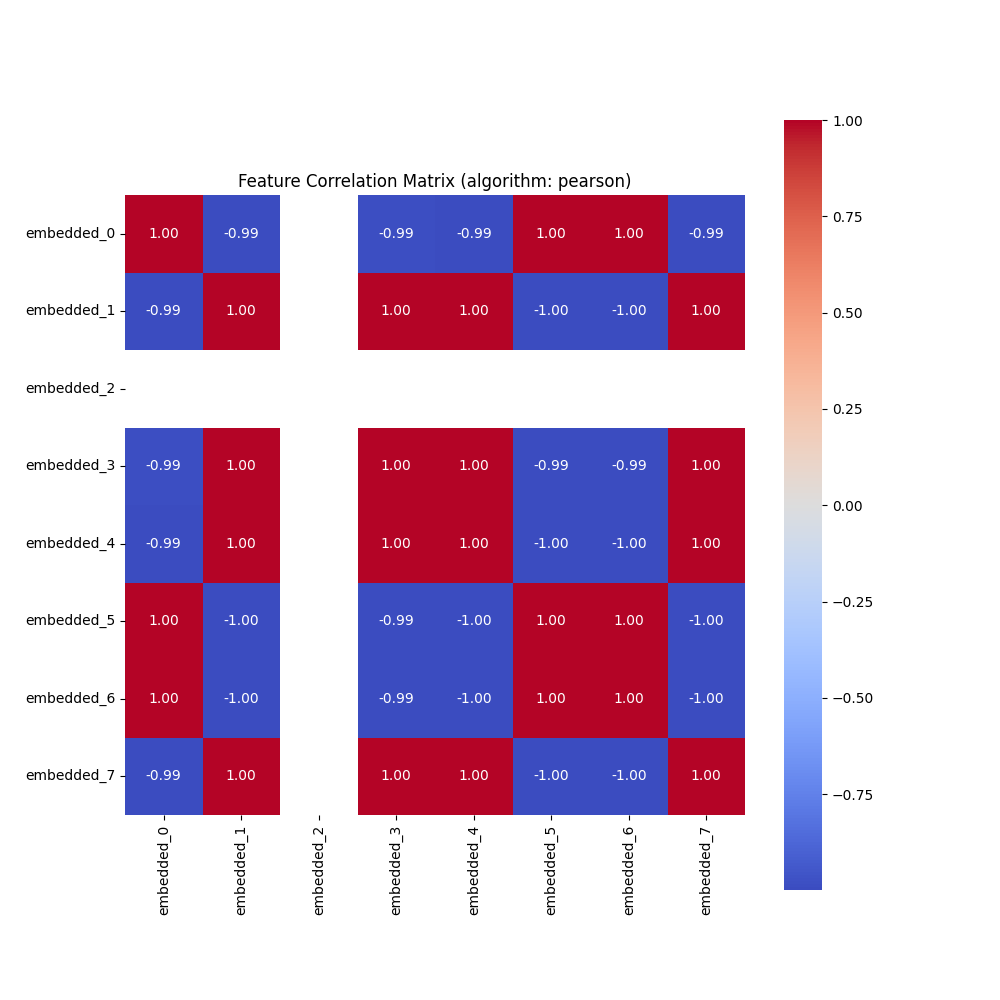
\includegraphics[width=0.8\linewidth]{img/annexes/27_filtered_chunk_extraction_-e_only-max-entropy_-s_activate/Transformers 6_correlation_matrix.png}} \\
\hline
\end{longtable}


\begin{longtable}{|c|c|}
\caption{Transformers 7 Feature Engineering Results on 27\_filtered\_chunk\_extraction\_-e\_only-max-entropy\_-s\_activate} \label{tab:27_filtered_chunk_extraction_-e_only-max-entropy_-s_activate_transformers_7_feature_engineering_results}\\
\hline
Dataset Name & 27\_filtered\_chunk\_extraction\_-e\_only-max-entropy\_-s\_activate \\ \hline
Instance & Transformers 7 \\ \hline
\multirow{8}{*}{Best Features} & embedded\_5 \\ \cline{2-2}
 & embedded\_11 \\ \cline{2-2}
 & embedded\_12 \\ \cline{2-2}
 & embedded\_13 \\ \cline{2-2}
 & embedded\_14 \\ \cline{2-2}
 & embedded\_15 \\ \cline{2-2}
 & embedded\_3 \\ \cline{2-2}
 & embedded\_4 \\ \cline{2-2}
\noalign{\vskip 5mm}
\multicolumn{2}{|c|}{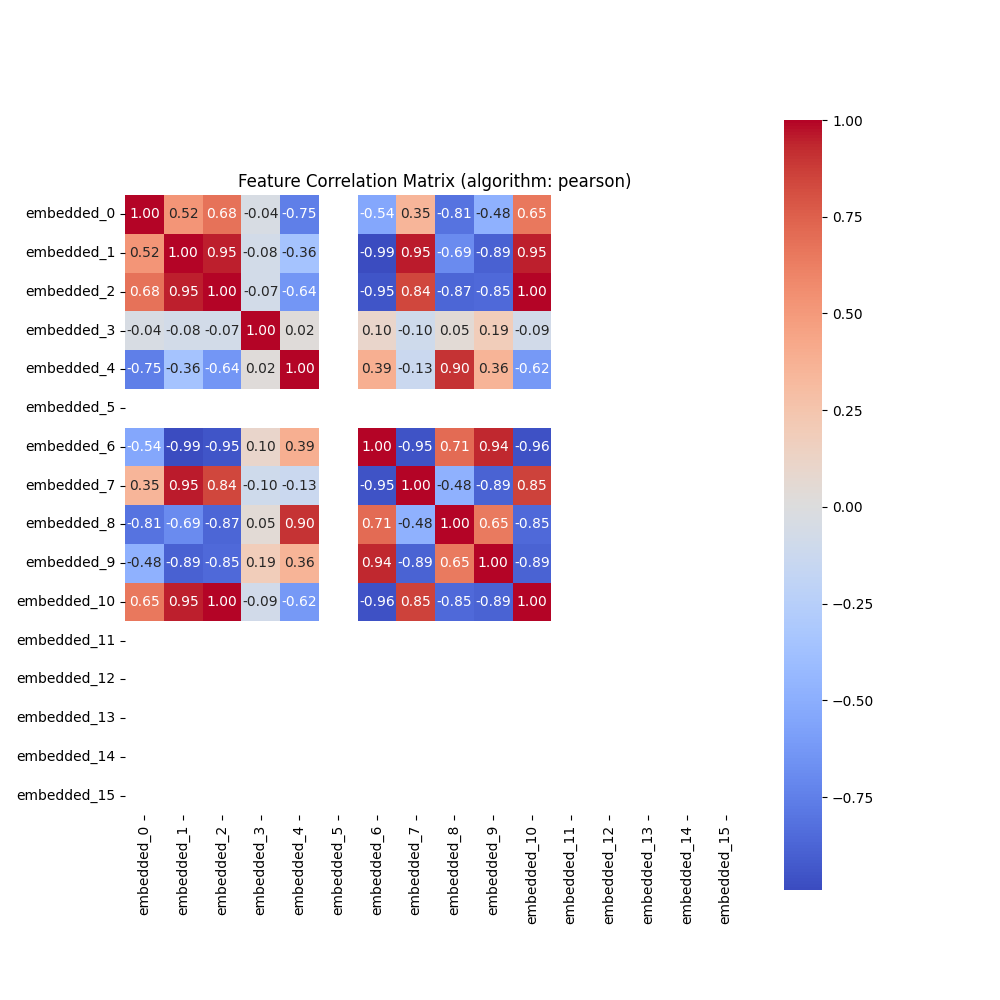
\includegraphics[width=0.8\linewidth]{img/annexes/27_filtered_chunk_extraction_-e_only-max-entropy_-s_activate/Transformers 7_correlation_matrix.png}} \\
\hline
\end{longtable}


\begin{longtable}{|c|c|}
\caption{Word2vec 0 Feature Engineering Results on 27\_filtered\_chunk\_extraction\_-e\_only-max-entropy\_-s\_activate} \label{tab:27_filtered_chunk_extraction_-e_only-max-entropy_-s_activate_word2vec_0_feature_engineering_results}\\
\hline
Dataset Name & 27\_filtered\_chunk\_extraction\_-e\_only-max-entropy\_-s\_activate \\ \hline
Instance & Word2vec 0 \\ \hline
\multirow{8}{*}{Best Features} & feature\_1 \\ \cline{2-2}
 & feature\_6 \\ \cline{2-2}
 & feature\_4 \\ \cline{2-2}
 & feature\_7 \\ \cline{2-2}
 & feature\_5 \\ \cline{2-2}
 & feature\_2 \\ \cline{2-2}
 & feature\_3 \\ \cline{2-2}
 & feature\_0 \\ \cline{2-2}
\noalign{\vskip 5mm}
\multicolumn{2}{|c|}{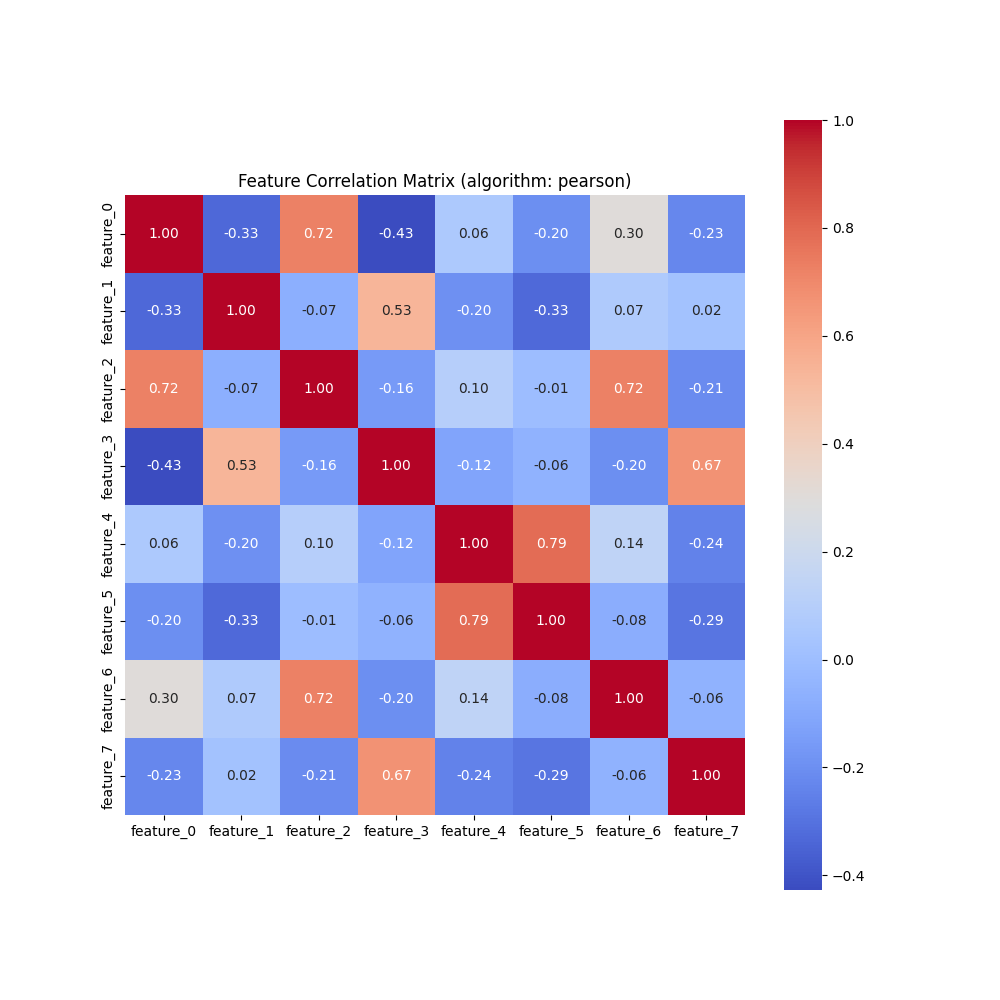
\includegraphics[width=0.8\linewidth]{img/annexes/27_filtered_chunk_extraction_-e_only-max-entropy_-s_activate/Word2vec 0_correlation_matrix.png}} \\
\hline
\end{longtable}


\begin{longtable}{|c|c|}
\caption{Word2vec 1 Feature Engineering Results on 27\_filtered\_chunk\_extraction\_-e\_only-max-entropy\_-s\_activate} \label{tab:27_filtered_chunk_extraction_-e_only-max-entropy_-s_activate_word2vec_1_feature_engineering_results}\\
\hline
Dataset Name & 27\_filtered\_chunk\_extraction\_-e\_only-max-entropy\_-s\_activate \\ \hline
Instance & Word2vec 1 \\ \hline
\multirow{8}{*}{Best Features} & feature\_3 \\ \cline{2-2}
 & feature\_2 \\ \cline{2-2}
 & feature\_6 \\ \cline{2-2}
 & feature\_4 \\ \cline{2-2}
 & feature\_0 \\ \cline{2-2}
 & feature\_7 \\ \cline{2-2}
 & feature\_1 \\ \cline{2-2}
 & feature\_5 \\ \cline{2-2}
\noalign{\vskip 5mm}
\multicolumn{2}{|c|}{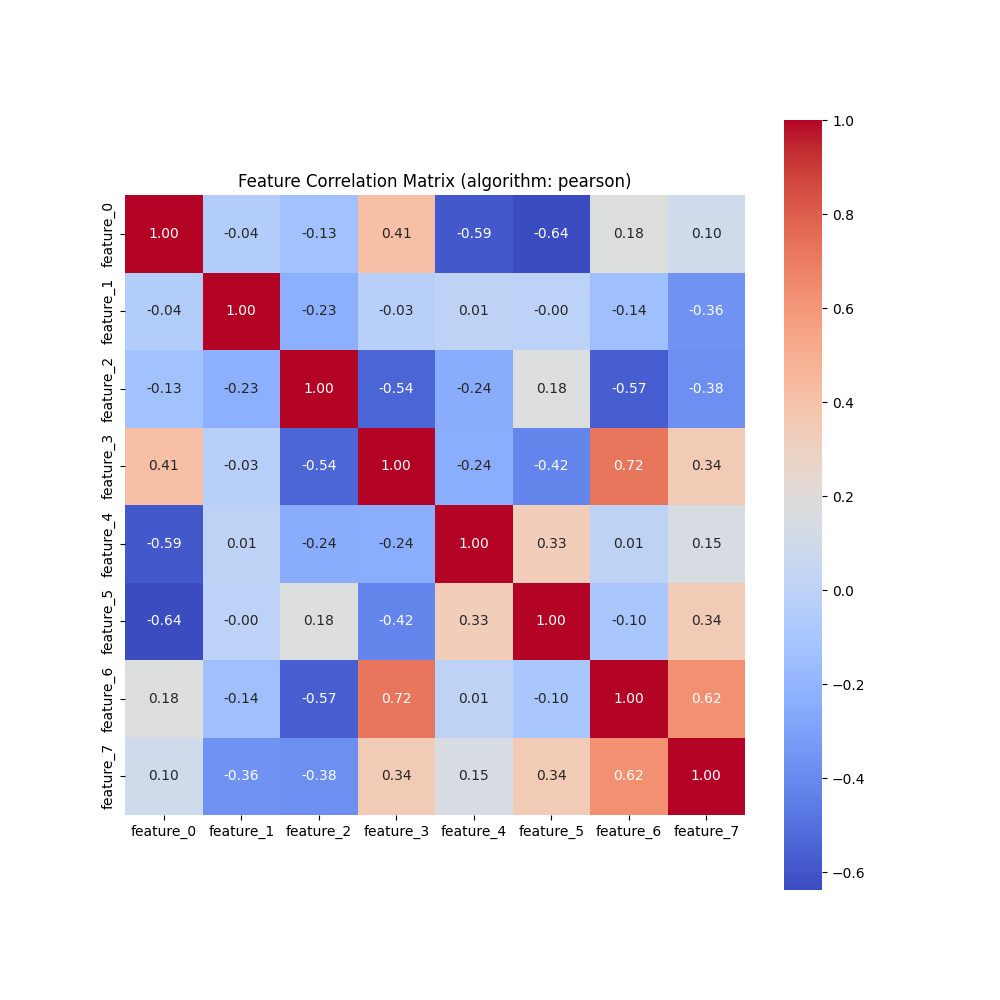
\includegraphics[width=0.8\linewidth]{img/annexes/27_filtered_chunk_extraction_-e_only-max-entropy_-s_activate/Word2vec 1_correlation_matrix.png}} \\
\hline
\end{longtable}


\begin{longtable}{|c|c|}
\caption{Word2vec 2 Feature Engineering Results on 27\_filtered\_chunk\_extraction\_-e\_only-max-entropy\_-s\_activate} \label{tab:27_filtered_chunk_extraction_-e_only-max-entropy_-s_activate_word2vec_2_feature_engineering_results}\\
\hline
Dataset Name & 27\_filtered\_chunk\_extraction\_-e\_only-max-entropy\_-s\_activate \\ \hline
Instance & Word2vec 2 \\ \hline
\multirow{8}{*}{Best Features} & feature\_2 \\ \cline{2-2}
 & feature\_7 \\ \cline{2-2}
 & feature\_1 \\ \cline{2-2}
 & feature\_4 \\ \cline{2-2}
 & feature\_5 \\ \cline{2-2}
 & feature\_6 \\ \cline{2-2}
 & feature\_3 \\ \cline{2-2}
 & feature\_0 \\ \cline{2-2}
\noalign{\vskip 5mm}
\multicolumn{2}{|c|}{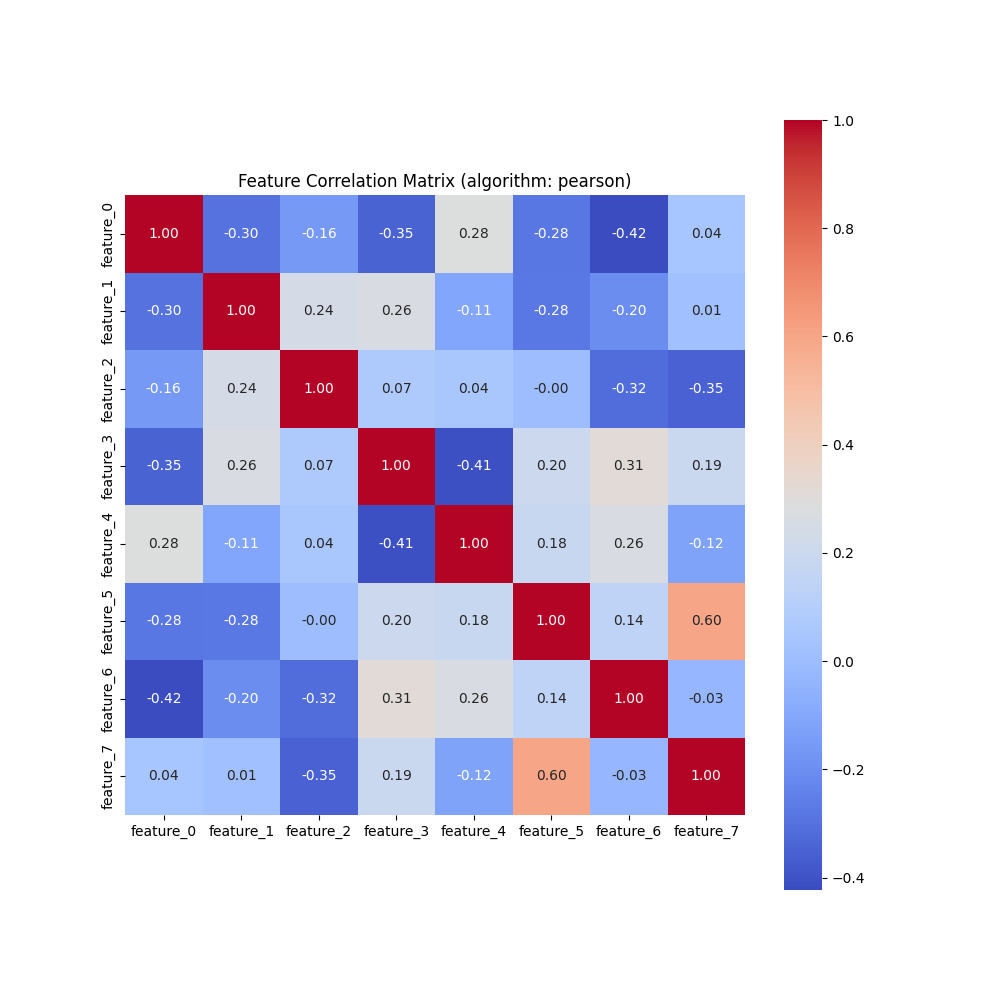
\includegraphics[width=0.8\linewidth]{img/annexes/27_filtered_chunk_extraction_-e_only-max-entropy_-s_activate/Word2vec 2_correlation_matrix.png}} \\
\hline
\end{longtable}


\begin{longtable}{|c|c|}
\caption{Word2vec 3 Feature Engineering Results on 27\_filtered\_chunk\_extraction\_-e\_only-max-entropy\_-s\_activate} \label{tab:27_filtered_chunk_extraction_-e_only-max-entropy_-s_activate_word2vec_3_feature_engineering_results}\\
\hline
Dataset Name & 27\_filtered\_chunk\_extraction\_-e\_only-max-entropy\_-s\_activate \\ \hline
Instance & Word2vec 3 \\ \hline
\multirow{8}{*}{Best Features} & feature\_4 \\ \cline{2-2}
 & feature\_3 \\ \cline{2-2}
 & feature\_1 \\ \cline{2-2}
 & feature\_2 \\ \cline{2-2}
 & feature\_0 \\ \cline{2-2}
 & feature\_6 \\ \cline{2-2}
 & feature\_7 \\ \cline{2-2}
 & feature\_5 \\ \cline{2-2}
\noalign{\vskip 5mm}
\multicolumn{2}{|c|}{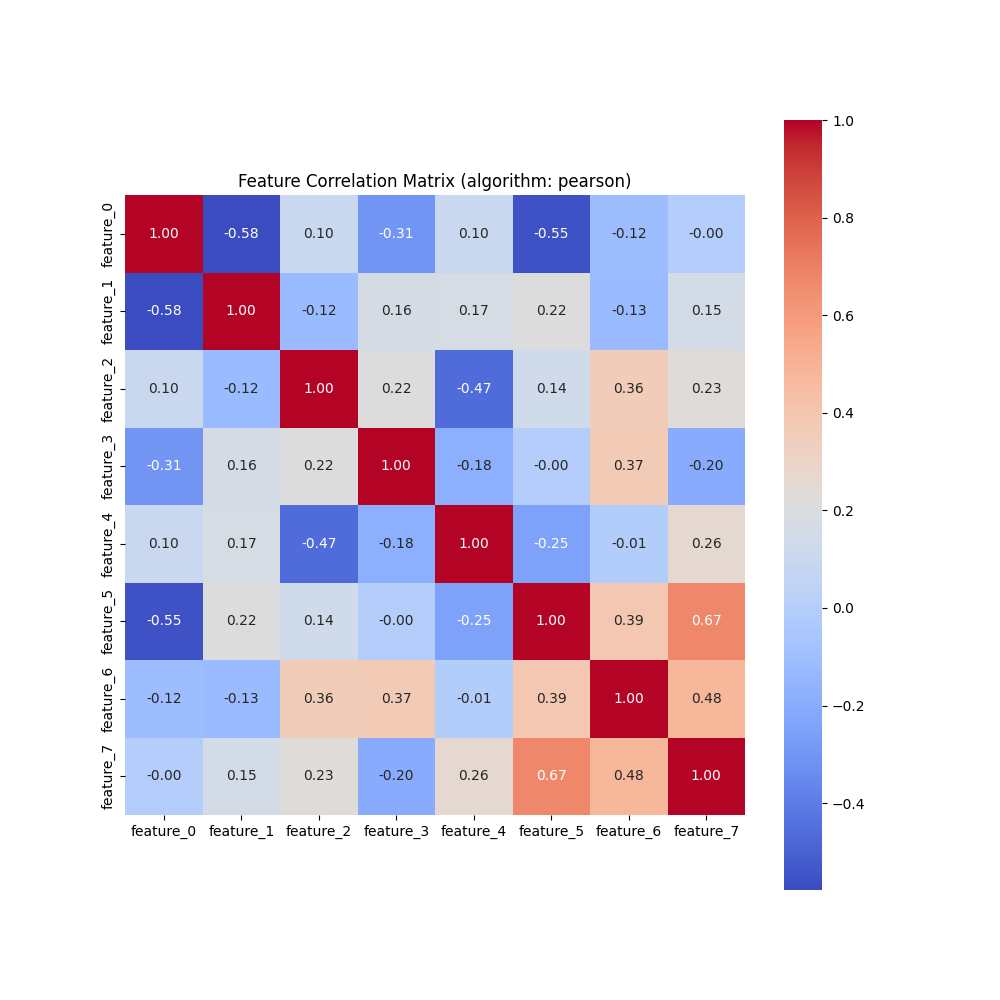
\includegraphics[width=0.8\linewidth]{img/annexes/27_filtered_chunk_extraction_-e_only-max-entropy_-s_activate/Word2vec 3_correlation_matrix.png}} \\
\hline
\end{longtable}


\begin{longtable}{|c|c|}
\caption{Word2vec 4 Feature Engineering Results on 27\_filtered\_chunk\_extraction\_-e\_only-max-entropy\_-s\_activate} \label{tab:27_filtered_chunk_extraction_-e_only-max-entropy_-s_activate_word2vec_4_feature_engineering_results}\\
\hline
Dataset Name & 27\_filtered\_chunk\_extraction\_-e\_only-max-entropy\_-s\_activate \\ \hline
Instance & Word2vec 4 \\ \hline
\multirow{8}{*}{Best Features} & feature\_8 \\ \cline{2-2}
 & feature\_11 \\ \cline{2-2}
 & feature\_9 \\ \cline{2-2}
 & feature\_10 \\ \cline{2-2}
 & feature\_0 \\ \cline{2-2}
 & feature\_1 \\ \cline{2-2}
 & feature\_13 \\ \cline{2-2}
 & feature\_2 \\ \cline{2-2}
\noalign{\vskip 5mm}
\multicolumn{2}{|c|}{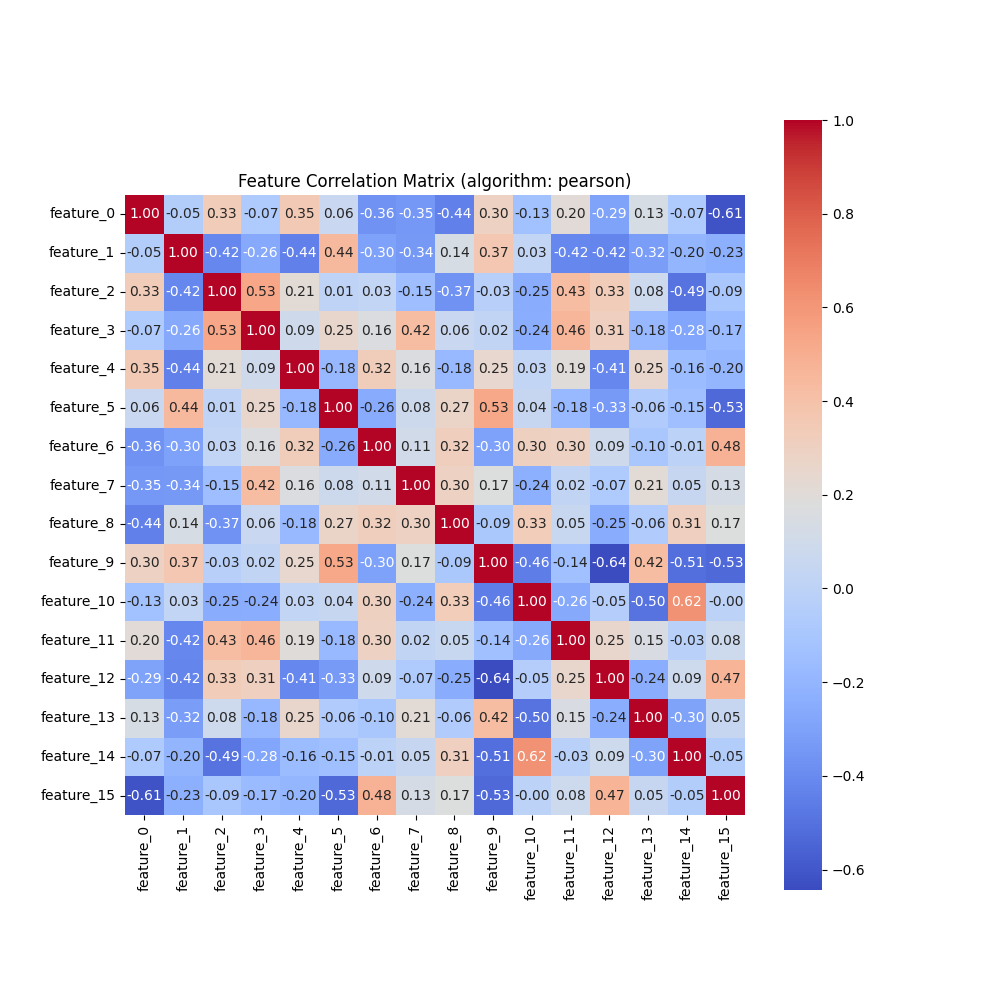
\includegraphics[width=0.8\linewidth]{img/annexes/27_filtered_chunk_extraction_-e_only-max-entropy_-s_activate/Word2vec 4_correlation_matrix.png}} \\
\hline
\end{longtable}


\begin{longtable}{|c|c|}
\caption{Word2vec 5 Feature Engineering Results on 27\_filtered\_chunk\_extraction\_-e\_only-max-entropy\_-s\_activate} \label{tab:27_filtered_chunk_extraction_-e_only-max-entropy_-s_activate_word2vec_5_feature_engineering_results}\\
\hline
Dataset Name & 27\_filtered\_chunk\_extraction\_-e\_only-max-entropy\_-s\_activate \\ \hline
Instance & Word2vec 5 \\ \hline
\multirow{8}{*}{Best Features} & feature\_12 \\ \cline{2-2}
 & feature\_8 \\ \cline{2-2}
 & feature\_3 \\ \cline{2-2}
 & feature\_0 \\ \cline{2-2}
 & feature\_7 \\ \cline{2-2}
 & feature\_2 \\ \cline{2-2}
 & feature\_14 \\ \cline{2-2}
 & feature\_4 \\ \cline{2-2}
\noalign{\vskip 5mm}
\multicolumn{2}{|c|}{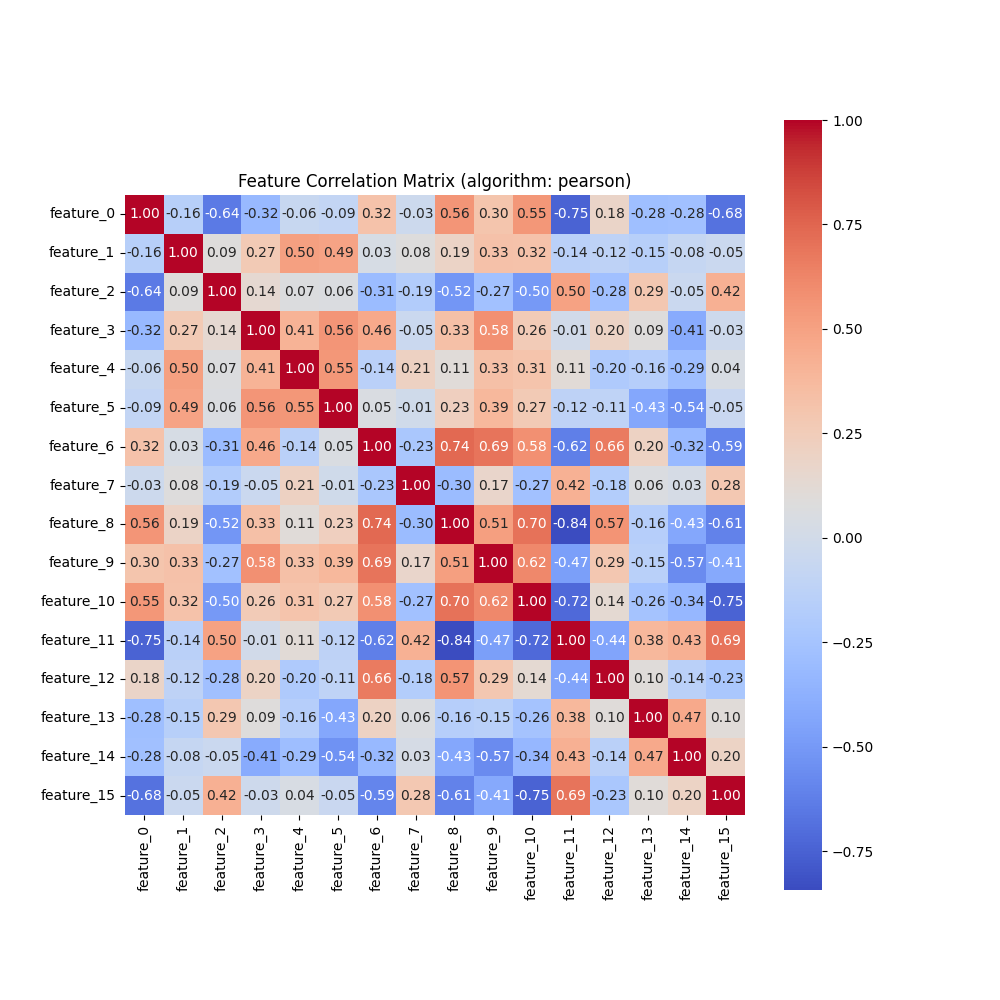
\includegraphics[width=0.8\linewidth]{img/annexes/27_filtered_chunk_extraction_-e_only-max-entropy_-s_activate/Word2vec 5_correlation_matrix.png}} \\
\hline
\end{longtable}


\begin{longtable}{|c|c|}
\caption{Word2vec 6 Feature Engineering Results on 27\_filtered\_chunk\_extraction\_-e\_only-max-entropy\_-s\_activate} \label{tab:27_filtered_chunk_extraction_-e_only-max-entropy_-s_activate_word2vec_6_feature_engineering_results}\\
\hline
Dataset Name & 27\_filtered\_chunk\_extraction\_-e\_only-max-entropy\_-s\_activate \\ \hline
Instance & Word2vec 6 \\ \hline
\multirow{8}{*}{Best Features} & feature\_11 \\ \cline{2-2}
 & feature\_3 \\ \cline{2-2}
 & feature\_12 \\ \cline{2-2}
 & feature\_14 \\ \cline{2-2}
 & feature\_13 \\ \cline{2-2}
 & feature\_8 \\ \cline{2-2}
 & feature\_5 \\ \cline{2-2}
 & feature\_6 \\ \cline{2-2}
\noalign{\vskip 5mm}
\multicolumn{2}{|c|}{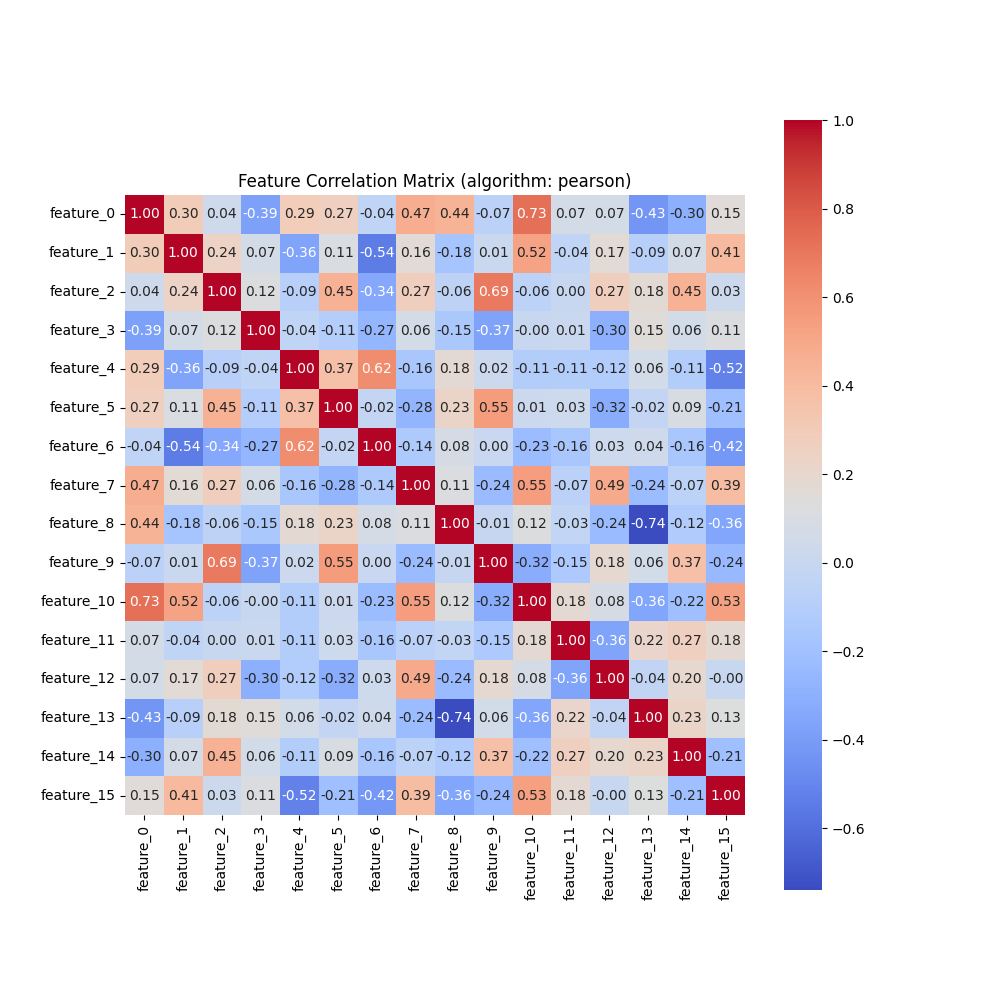
\includegraphics[width=0.8\linewidth]{img/annexes/27_filtered_chunk_extraction_-e_only-max-entropy_-s_activate/Word2vec 6_correlation_matrix.png}} \\
\hline
\end{longtable}


\begin{longtable}{|c|c|}
\caption{Word2vec 7 Feature Engineering Results on 27\_filtered\_chunk\_extraction\_-e\_only-max-entropy\_-s\_activate} \label{tab:27_filtered_chunk_extraction_-e_only-max-entropy_-s_activate_word2vec_7_feature_engineering_results}\\
\hline
Dataset Name & 27\_filtered\_chunk\_extraction\_-e\_only-max-entropy\_-s\_activate \\ \hline
Instance & Word2vec 7 \\ \hline
\multirow{8}{*}{Best Features} & feature\_5 \\ \cline{2-2}
 & feature\_12 \\ \cline{2-2}
 & feature\_2 \\ \cline{2-2}
 & feature\_3 \\ \cline{2-2}
 & feature\_6 \\ \cline{2-2}
 & feature\_14 \\ \cline{2-2}
 & feature\_13 \\ \cline{2-2}
 & feature\_11 \\ \cline{2-2}
\noalign{\vskip 5mm}
\multicolumn{2}{|c|}{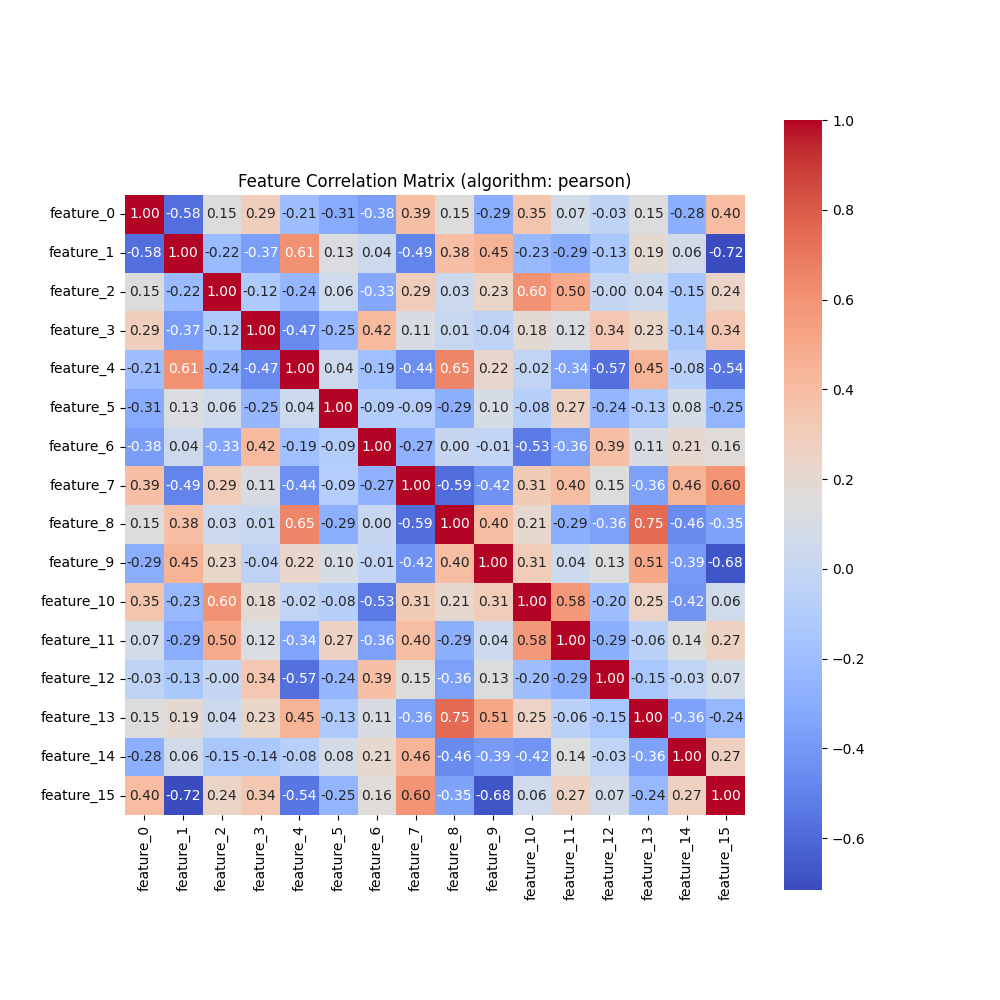
\includegraphics[width=0.8\linewidth]{img/annexes/27_filtered_chunk_extraction_-e_only-max-entropy_-s_activate/Word2vec 7_correlation_matrix.png}} \\
\hline
\end{longtable}


\begin{longtable}{|c|c|}
\caption{Word2vec 8 Feature Engineering Results on 27\_filtered\_chunk\_extraction\_-e\_only-max-entropy\_-s\_activate} \label{tab:27_filtered_chunk_extraction_-e_only-max-entropy_-s_activate_word2vec_8_feature_engineering_results}\\
\hline
Dataset Name & 27\_filtered\_chunk\_extraction\_-e\_only-max-entropy\_-s\_activate \\ \hline
Instance & Word2vec 8 \\ \hline
\multirow{8}{*}{Best Features} & feature\_33 \\ \cline{2-2}
 & feature\_61 \\ \cline{2-2}
 & feature\_86 \\ \cline{2-2}
 & feature\_93 \\ \cline{2-2}
 & feature\_70 \\ \cline{2-2}
 & feature\_32 \\ \cline{2-2}
 & feature\_10 \\ \cline{2-2}
 & feature\_42 \\ \cline{2-2}
\noalign{\vskip 5mm}
\multicolumn{2}{|c|}{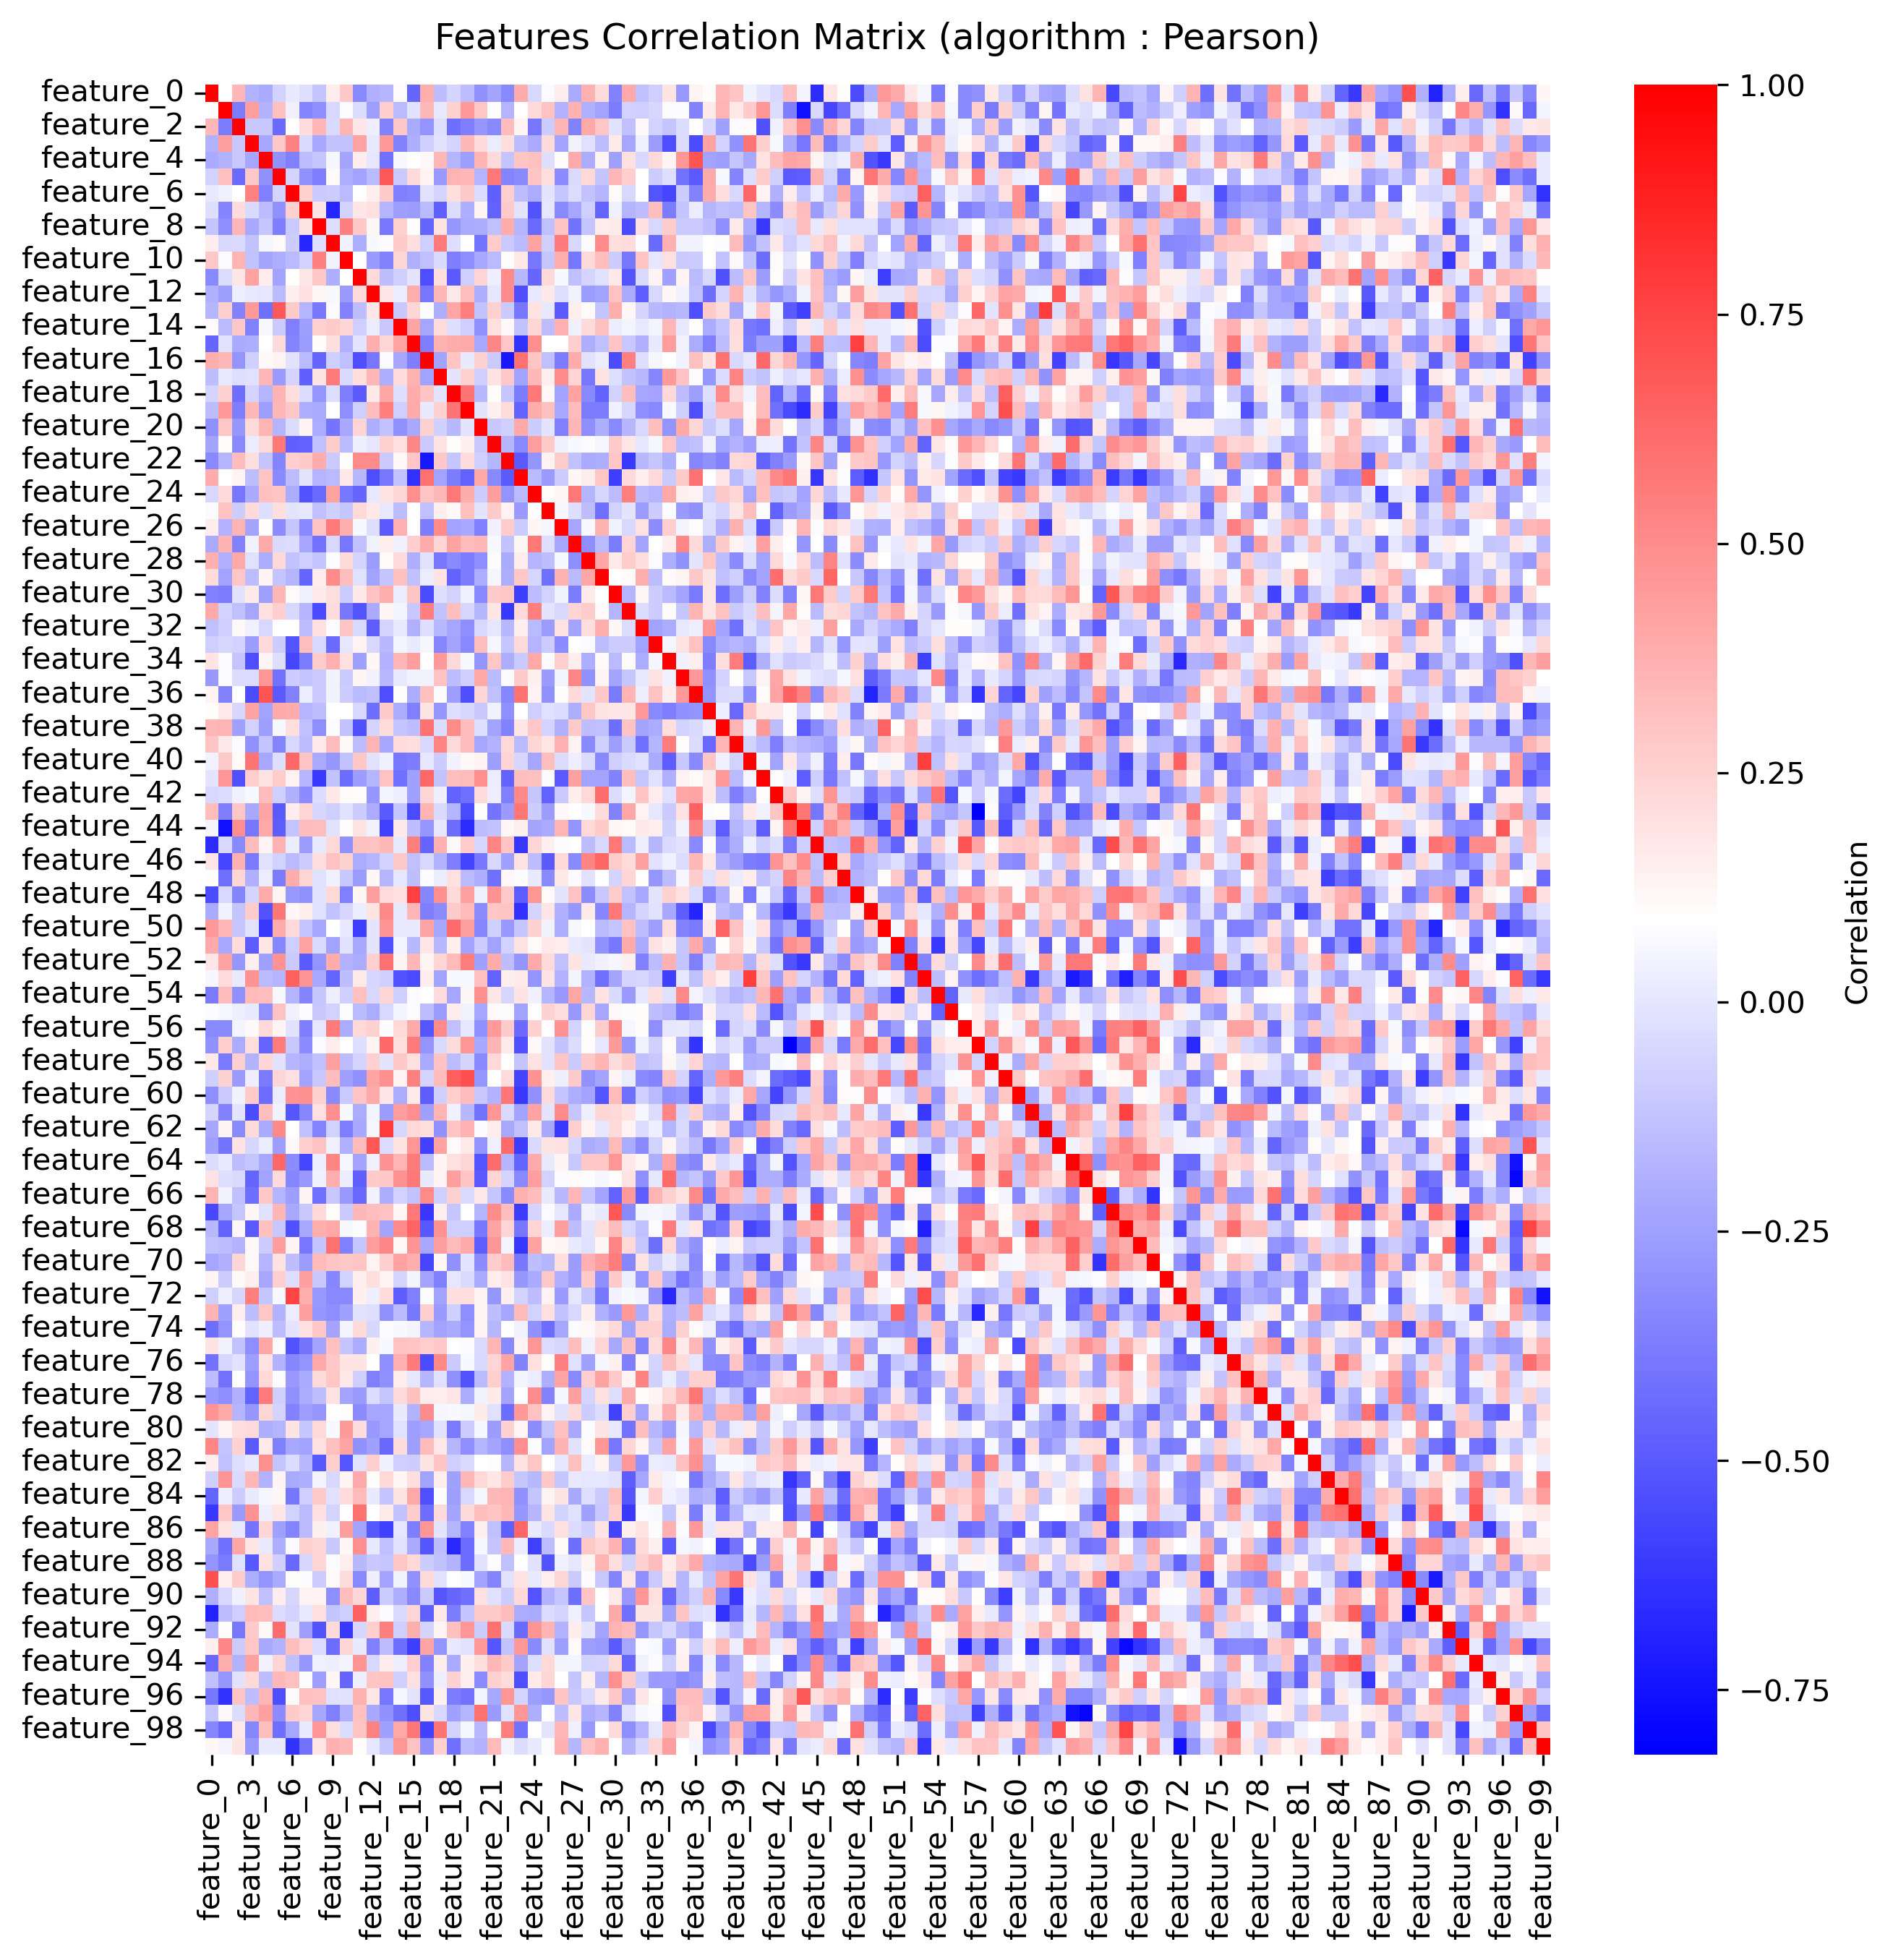
\includegraphics[width=0.8\linewidth]{img/annexes/27_filtered_chunk_extraction_-e_only-max-entropy_-s_activate/Word2vec 8_correlation_matrix.png}} \\
\hline
\end{longtable}


\begin{longtable}{|c|c|}
\caption{Word2vec 9 Feature Engineering Results on 27\_filtered\_chunk\_extraction\_-e\_only-max-entropy\_-s\_activate} \label{tab:27_filtered_chunk_extraction_-e_only-max-entropy_-s_activate_word2vec_9_feature_engineering_results}\\
\hline
Dataset Name & 27\_filtered\_chunk\_extraction\_-e\_only-max-entropy\_-s\_activate \\ \hline
Instance & Word2vec 9 \\ \hline
\multirow{8}{*}{Best Features} & feature\_15 \\ \cline{2-2}
 & feature\_16 \\ \cline{2-2}
 & feature\_69 \\ \cline{2-2}
 & feature\_57 \\ \cline{2-2}
 & feature\_30 \\ \cline{2-2}
 & feature\_75 \\ \cline{2-2}
 & feature\_28 \\ \cline{2-2}
 & feature\_42 \\ \cline{2-2}
\noalign{\vskip 5mm}
\multicolumn{2}{|c|}{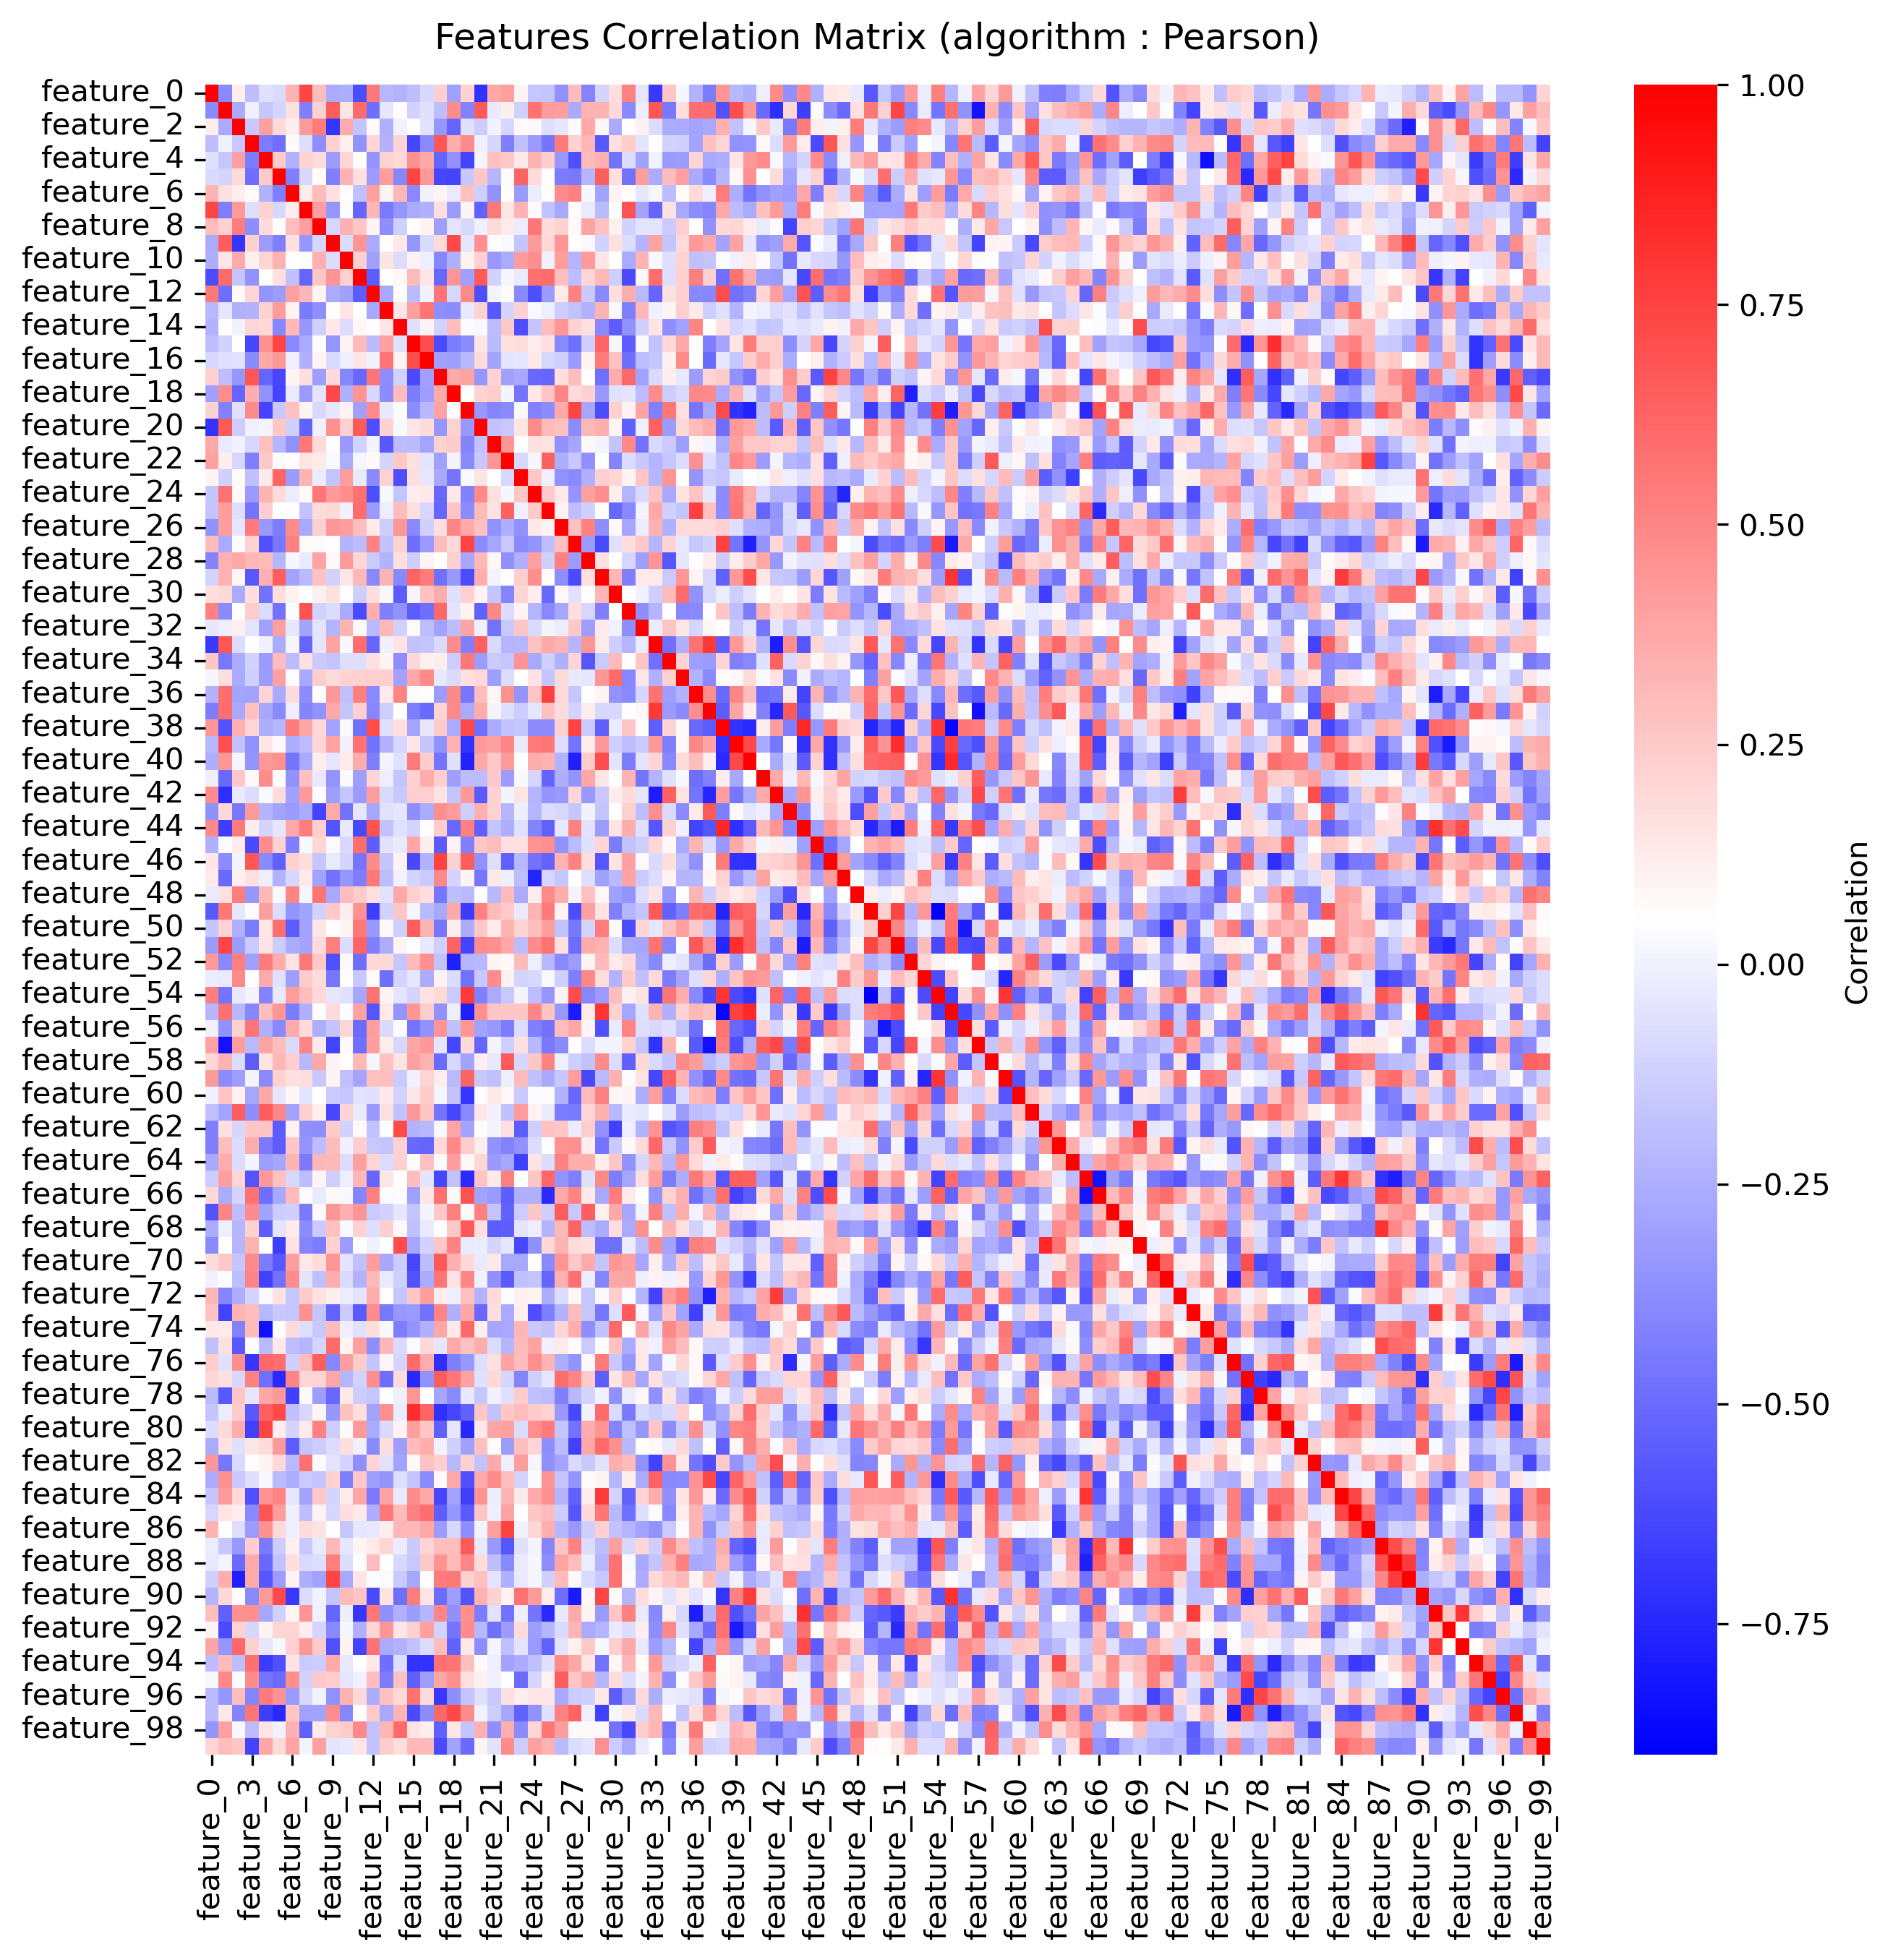
\includegraphics[width=0.8\linewidth]{img/annexes/27_filtered_chunk_extraction_-e_only-max-entropy_-s_activate/Word2vec 9_correlation_matrix.png}} \\
\hline
\end{longtable}


\begin{longtable}{|c|c|}
\caption{Word2vec 10 Feature Engineering Results on 27\_filtered\_chunk\_extraction\_-e\_only-max-entropy\_-s\_activate} \label{tab:27_filtered_chunk_extraction_-e_only-max-entropy_-s_activate_word2vec_10_feature_engineering_results}\\
\hline
Dataset Name & 27\_filtered\_chunk\_extraction\_-e\_only-max-entropy\_-s\_activate \\ \hline
Instance & Word2vec 10 \\ \hline
\multirow{8}{*}{Best Features} & feature\_78 \\ \cline{2-2}
 & feature\_25 \\ \cline{2-2}
 & feature\_10 \\ \cline{2-2}
 & feature\_86 \\ \cline{2-2}
 & feature\_68 \\ \cline{2-2}
 & feature\_92 \\ \cline{2-2}
 & feature\_71 \\ \cline{2-2}
 & feature\_12 \\ \cline{2-2}
\noalign{\vskip 5mm}
\multicolumn{2}{|c|}{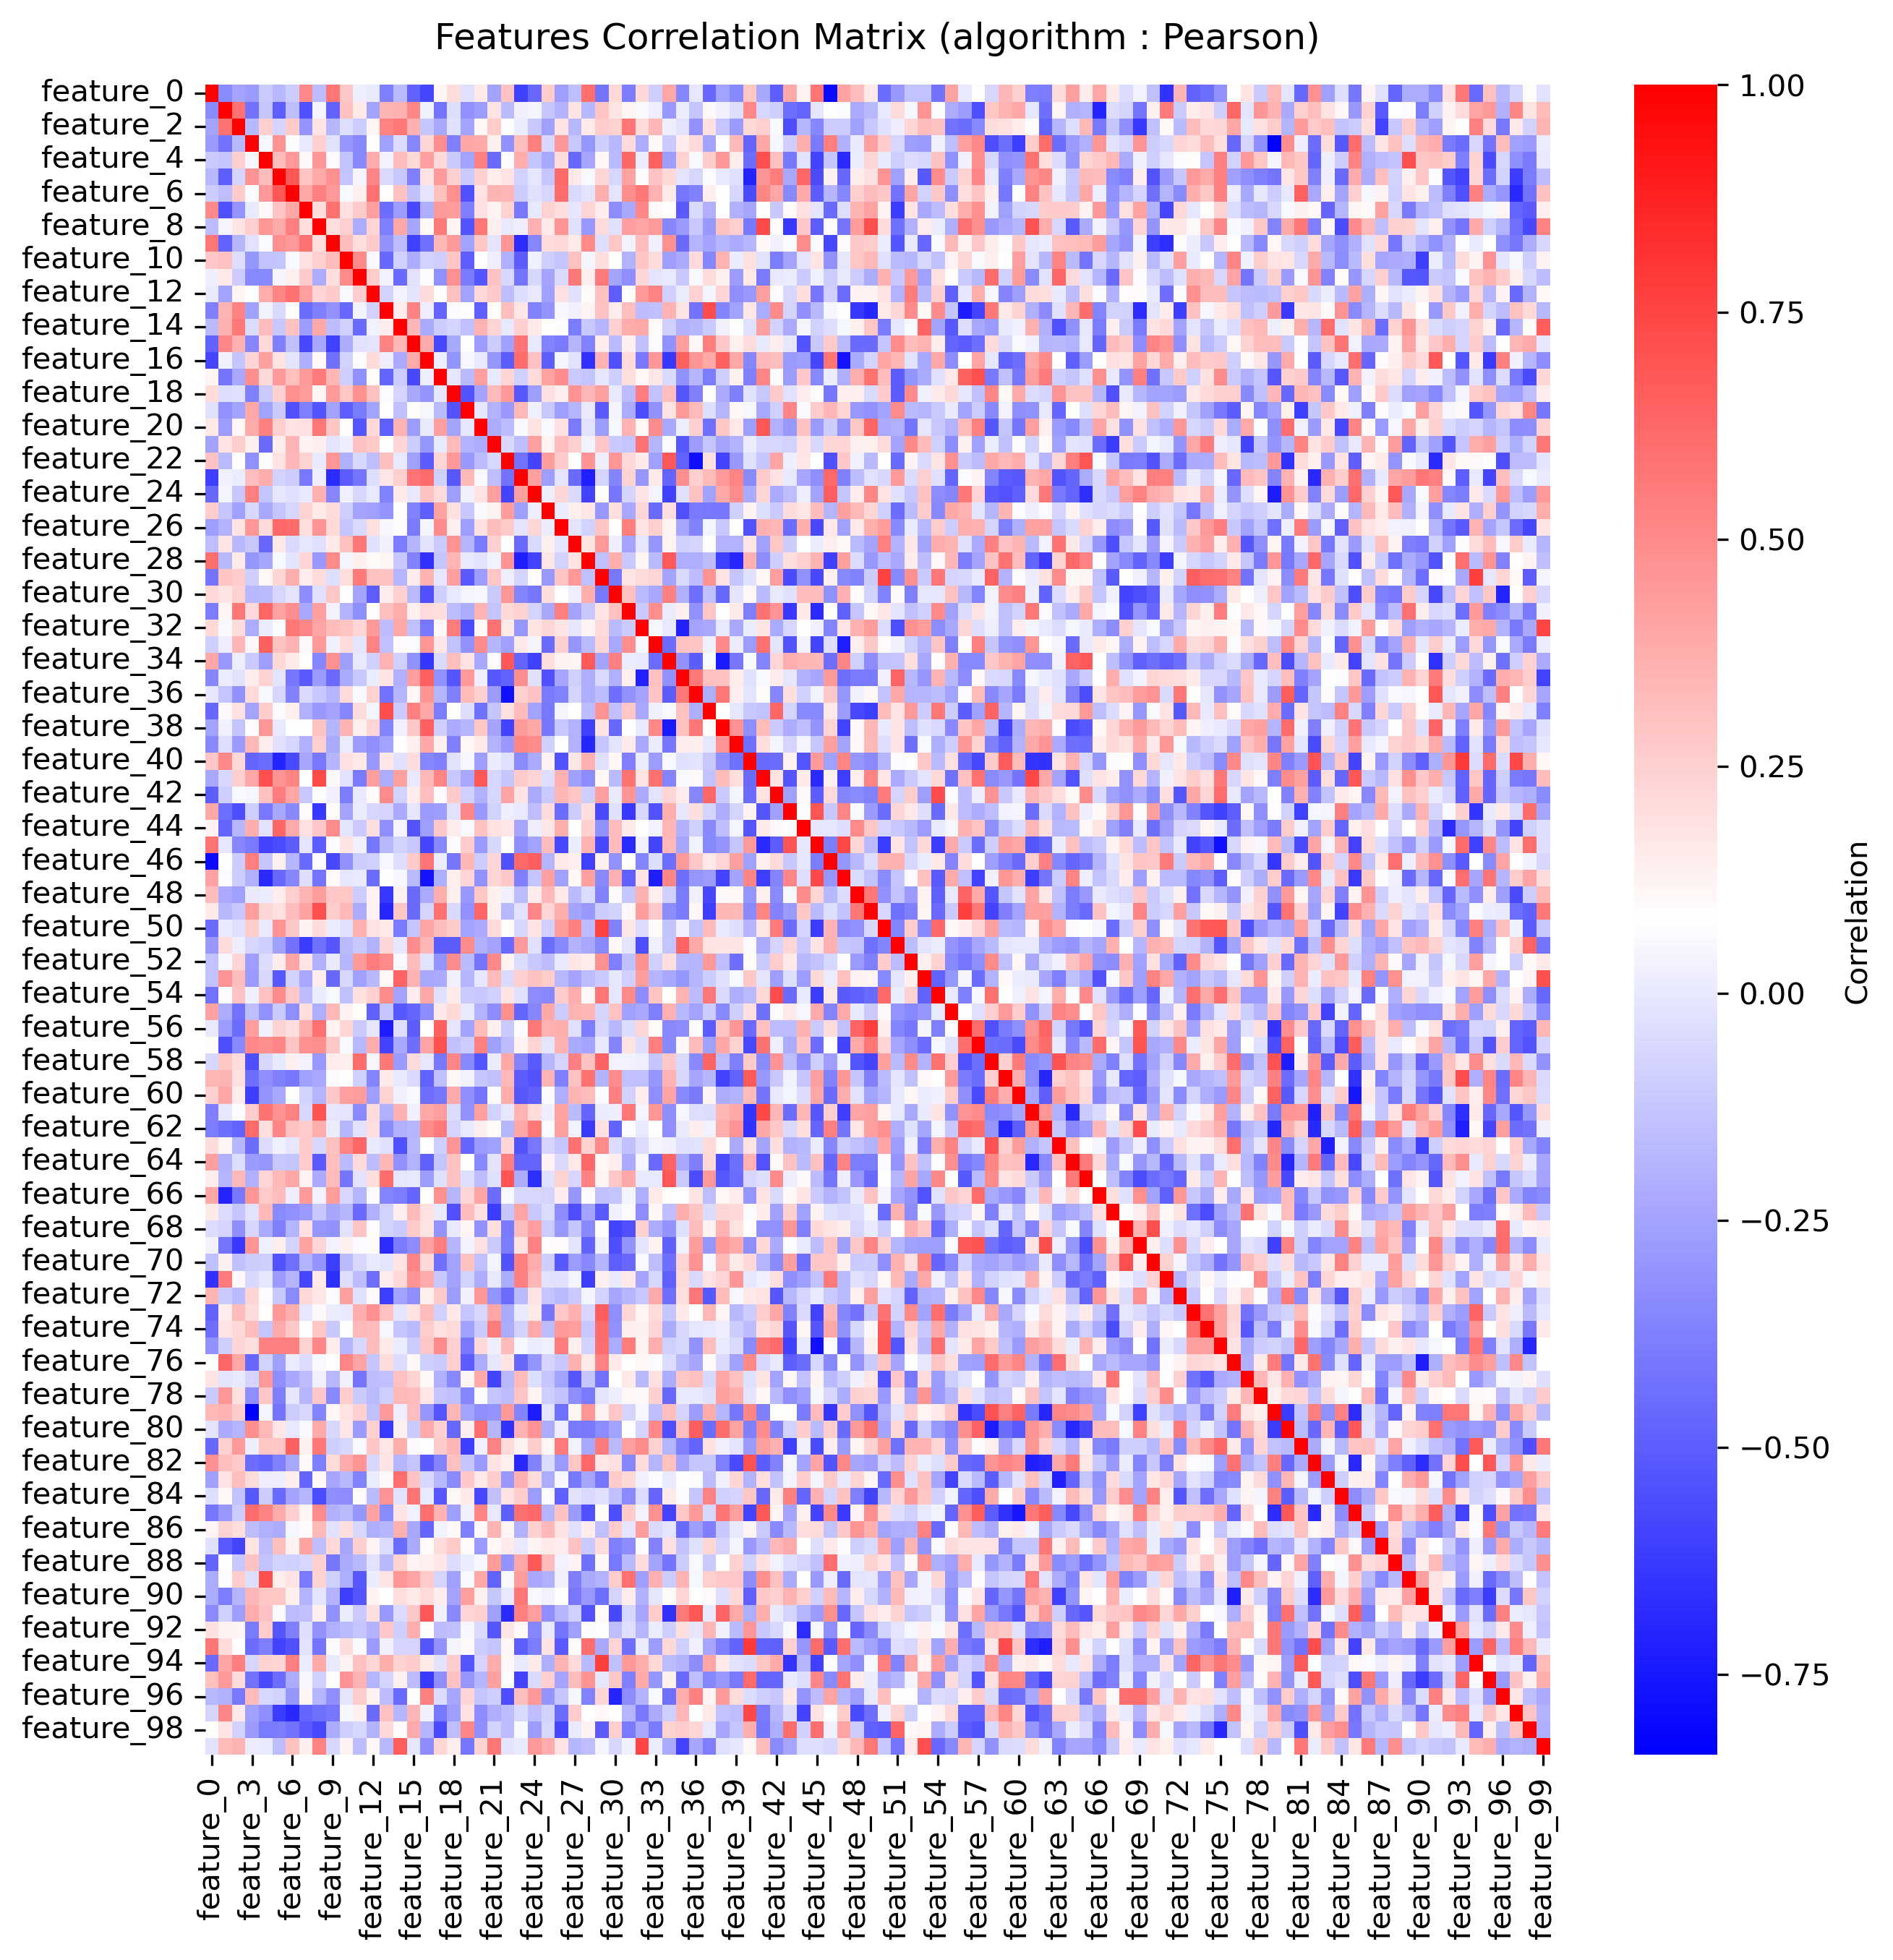
\includegraphics[width=0.8\linewidth]{img/annexes/27_filtered_chunk_extraction_-e_only-max-entropy_-s_activate/Word2vec 10_correlation_matrix.png}} \\
\hline
\end{longtable}


\begin{longtable}{|c|c|}
\caption{Word2vec 11 Feature Engineering Results on 27\_filtered\_chunk\_extraction\_-e\_only-max-entropy\_-s\_activate} \label{tab:27_filtered_chunk_extraction_-e_only-max-entropy_-s_activate_word2vec_11_feature_engineering_results}\\
\hline
Dataset Name & 27\_filtered\_chunk\_extraction\_-e\_only-max-entropy\_-s\_activate \\ \hline
Instance & Word2vec 11 \\ \hline
\multirow{8}{*}{Best Features} & feature\_28 \\ \cline{2-2}
 & feature\_39 \\ \cline{2-2}
 & feature\_84 \\ \cline{2-2}
 & feature\_76 \\ \cline{2-2}
 & feature\_89 \\ \cline{2-2}
 & feature\_77 \\ \cline{2-2}
 & feature\_50 \\ \cline{2-2}
 & feature\_95 \\ \cline{2-2}
\noalign{\vskip 5mm}
\multicolumn{2}{|c|}{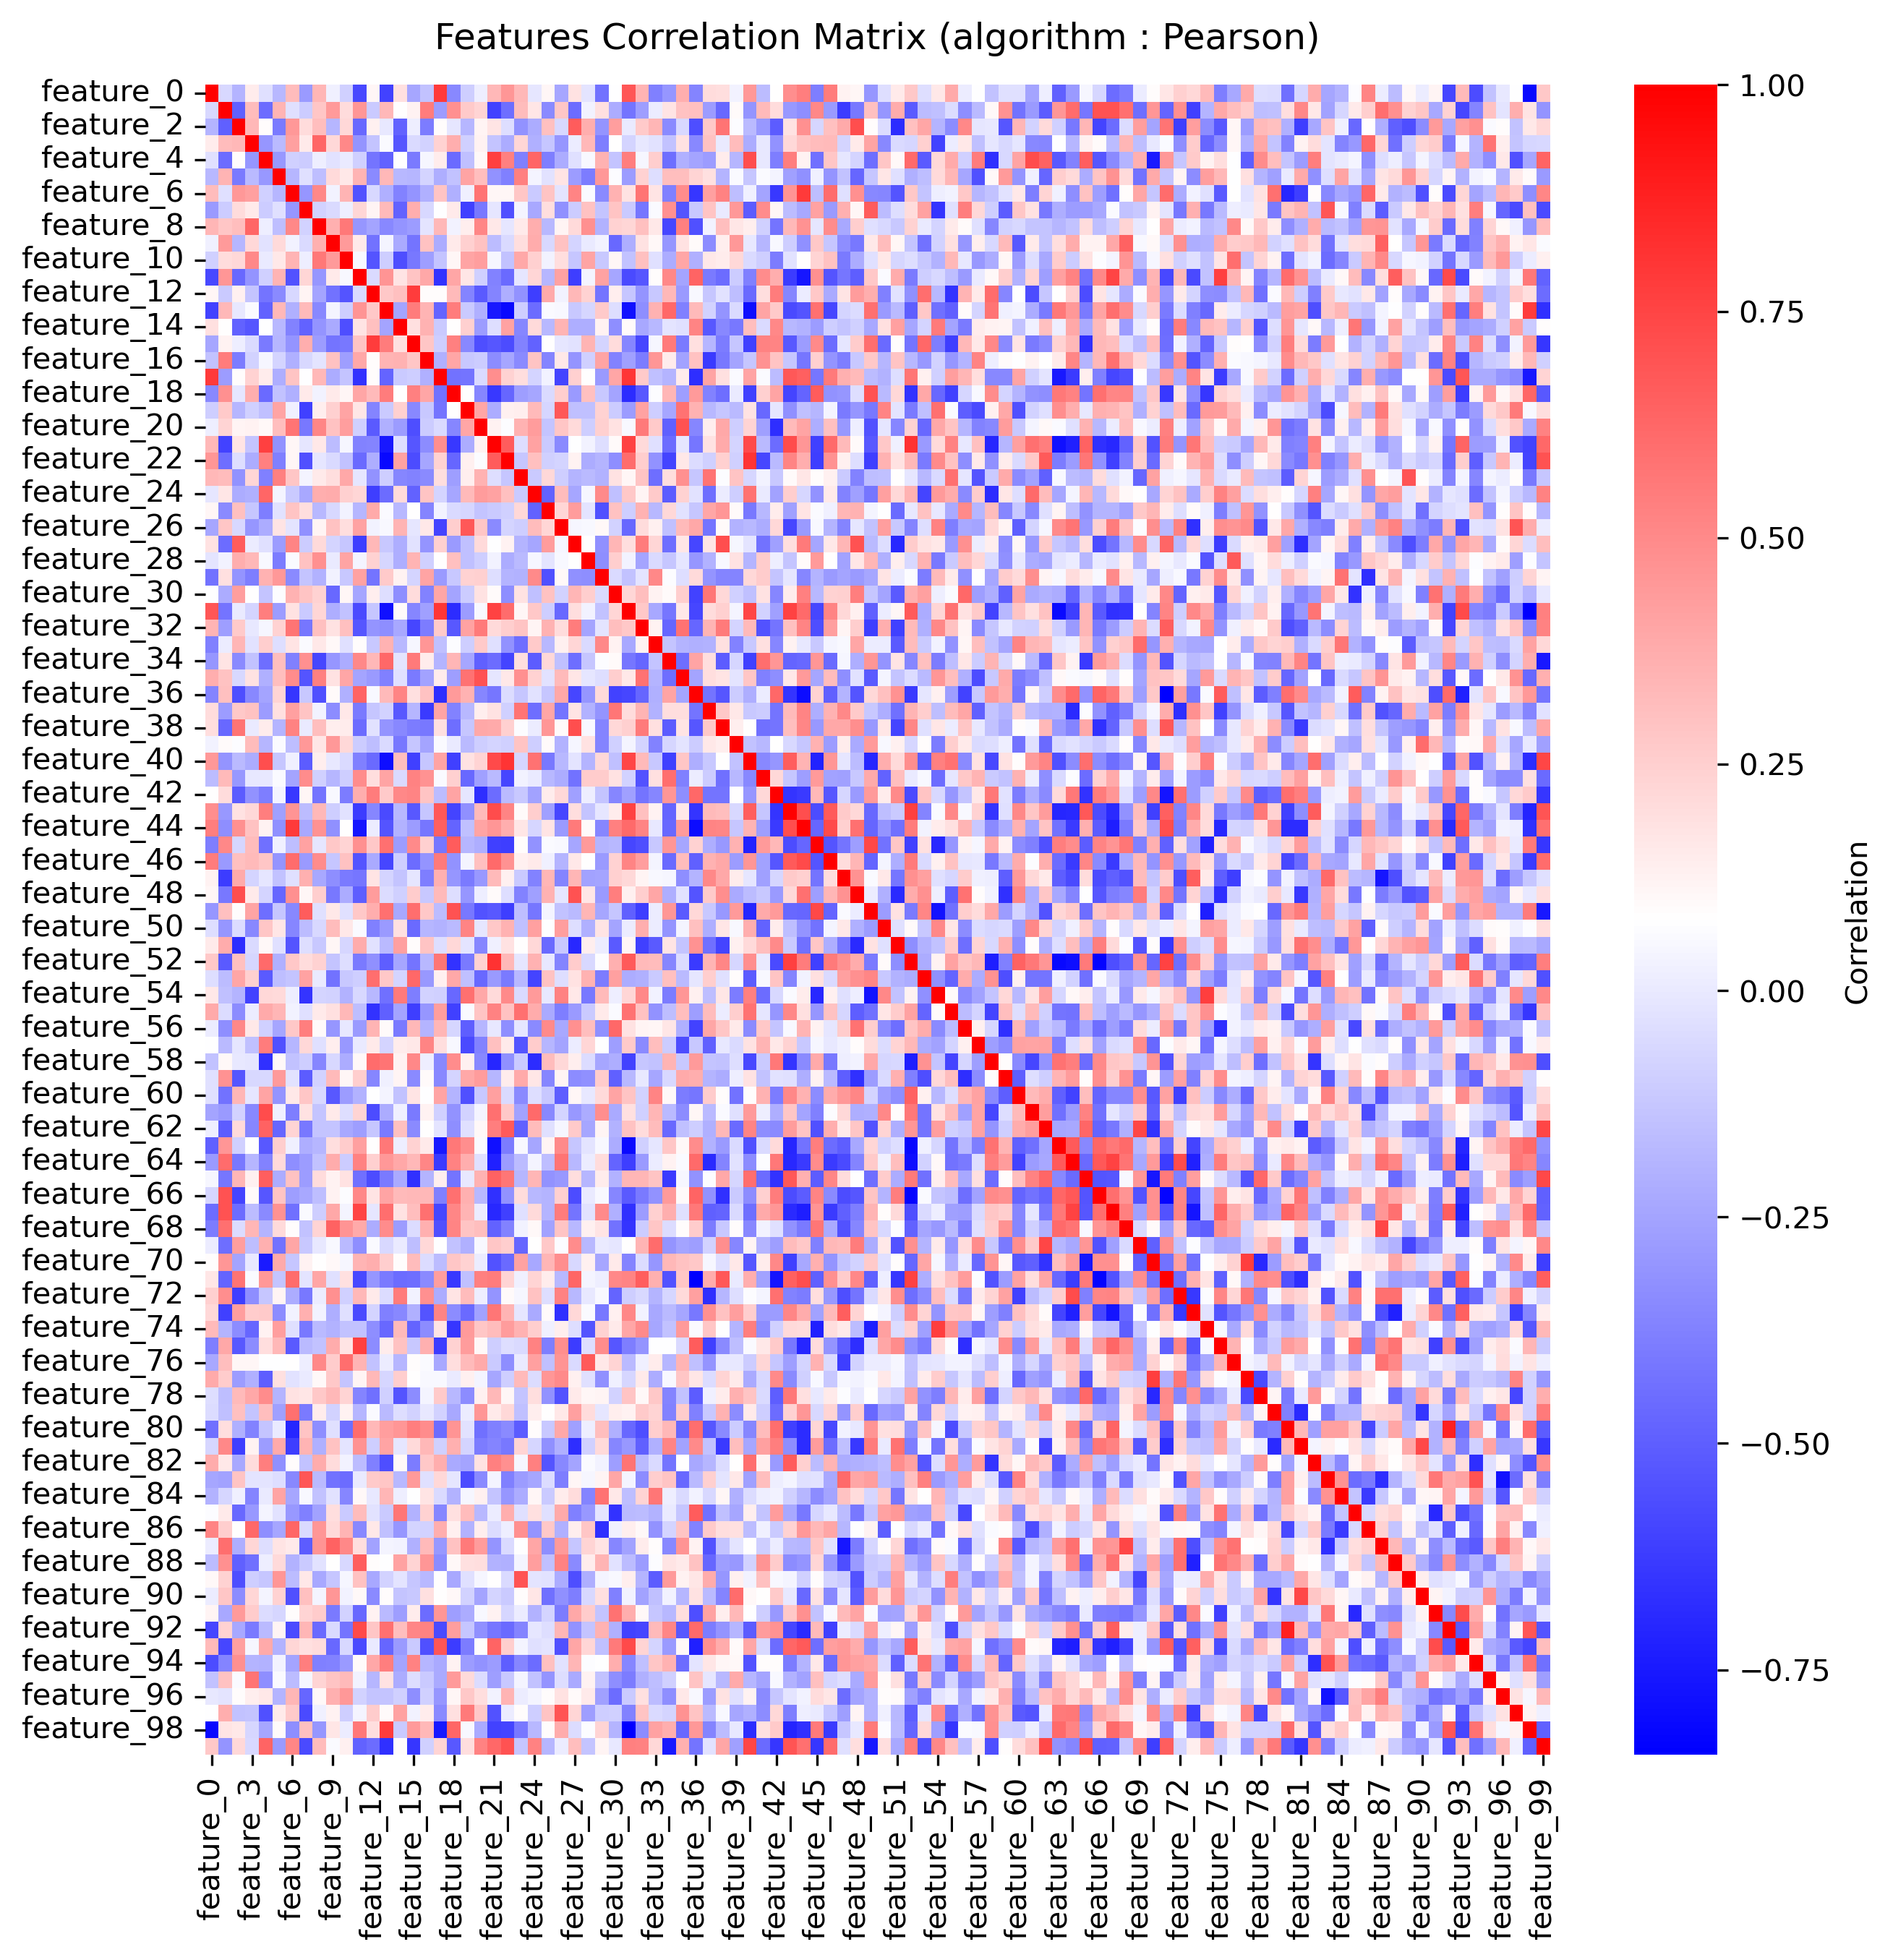
\includegraphics[width=0.8\linewidth]{img/annexes/27_filtered_chunk_extraction_-e_only-max-entropy_-s_activate/Word2vec 11_correlation_matrix.png}} \\
\hline
\end{longtable}


\section{Clustering results}

\label{sec:annexe:clustering_results}

\subsection{25\_filtered\_chunk\_extraction\_-e\_none\_-s\_activate}

\begin{longtable}{|c|c|c|c|c|}
\caption{Word2vec 0 Clustering Results on 25\_filtered\_chunk\_extraction\_-e\_none\_-s\_activate} \label{tab:25_filtered_chunk_extraction_-e_none_-s_activate_word2vec_0_clustering_results}\\
\hline
\multicolumn{5}{|c|}{\textbf{General Information}} \\
\hline
\multicolumn{2}{|c|}{Min Samples} & \multicolumn{3}{c|}{937} \\
\multicolumn{2}{|c|}{Total Duration} & \multicolumn{3}{c|}{3327.69158 s} \\
\hline
\multicolumn{5}{|c|}{\textbf{Clustering Information}} \\
\hline
EPS & Number of Clusters & Silhouette Score & Noise Points & Duration \\
0.01 & 1 & None & None & 657.12882 s\\
0.02 & 1 & None & None & 666.575554 s\\
0.03 & 1 & None & None & 674.458977 s\\
0.04 & 1 & None & None & 668.369706 s\\
0.05 & 1 & None & None & 661.124915 s\\
\hline
\multicolumn{5}{|c|}{\textbf{Label Association}} \\
\hline
Cluster ID & \multicolumn{2}{c|}{Label} & \multicolumn{2}{c|}{Number of Samples} \\
\hline
\end{longtable}


\begin{longtable}{|c|c|c|c|c|}
\caption{Word2vec 1 Clustering Results on 25\_filtered\_chunk\_extraction\_-e\_none\_-s\_activate} \label{tab:25_filtered_chunk_extraction_-e_none_-s_activate_word2vec_1_clustering_results}\\
\hline
\multicolumn{5}{|c|}{\textbf{General Information}} \\
\hline
\multicolumn{2}{|c|}{Min Samples} & \multicolumn{3}{c|}{937} \\
\multicolumn{2}{|c|}{Total Duration} & \multicolumn{3}{c|}{3739.764487 s} \\
\hline
\multicolumn{5}{|c|}{\textbf{Clustering Information}} \\
\hline
EPS & Number of Clusters & Silhouette Score & Noise Points & Duration \\
0.01 & 1 & None & None & 774.223486 s\\
0.02 & 1 & None & None & 741.354391 s\\
0.03 & 1 & None & None & 731.504657 s\\
0.04 & 1 & None & None & 740.939556 s\\
0.05 & 1 & None & None & 751.715116 s\\
\hline
\multicolumn{5}{|c|}{\textbf{Label Association}} \\
\hline
Cluster ID & \multicolumn{2}{c|}{Label} & \multicolumn{2}{c|}{Number of Samples} \\
\hline
\end{longtable}


\begin{longtable}{|c|c|c|c|c|}
\caption{Word2vec 2 Clustering Results on 25\_filtered\_chunk\_extraction\_-e\_none\_-s\_activate} \label{tab:25_filtered_chunk_extraction_-e_none_-s_activate_word2vec_2_clustering_results}\\
\hline
\multicolumn{5}{|c|}{\textbf{General Information}} \\
\hline
\multicolumn{2}{|c|}{Min Samples} & \multicolumn{3}{c|}{937} \\
\multicolumn{2}{|c|}{Total Duration} & \multicolumn{3}{c|}{3869.848014 s} \\
\hline
\multicolumn{5}{|c|}{\textbf{Clustering Information}} \\
\hline
EPS & Number of Clusters & Silhouette Score & Noise Points & Duration \\
0.01 & 1 & None & None & 786.426559 s\\
0.02 & 1 & None & None & 803.378659 s\\
0.03 & 1 & None & None & 738.827762 s\\
0.04 & 1 & None & None & 779.099225 s\\
0.05 & 1 & None & None & 762.080643 s\\
\hline
\multicolumn{5}{|c|}{\textbf{Label Association}} \\
\hline
Cluster ID & \multicolumn{2}{c|}{Label} & \multicolumn{2}{c|}{Number of Samples} \\
\hline
\end{longtable}


\begin{longtable}{|c|c|c|c|c|}
\caption{Word2vec 3 Clustering Results on 25\_filtered\_chunk\_extraction\_-e\_none\_-s\_activate} \label{tab:25_filtered_chunk_extraction_-e_none_-s_activate_word2vec_3_clustering_results}\\
\hline
\multicolumn{5}{|c|}{\textbf{General Information}} \\
\hline
\multicolumn{2}{|c|}{Min Samples} & \multicolumn{3}{c|}{937} \\
\multicolumn{2}{|c|}{Total Duration} & \multicolumn{3}{c|}{3634.492193 s} \\
\hline
\multicolumn{5}{|c|}{\textbf{Clustering Information}} \\
\hline
EPS & Number of Clusters & Silhouette Score & Noise Points & Duration \\
0.01 & 2 & 0.21665062010288239 & 3676 & 747.692523 s\\
0.02 & 1 & None & None & 697.073419 s\\
0.03 & 1 & None & None & 694.980969 s\\
0.04 & 1 & None & None & 737.728848 s\\
0.05 & 1 & None & None & 756.257249 s\\
\hline
\multicolumn{5}{|c|}{\textbf{Best EPS Information}} \\
\hline
0.01 & 2 & 0.21665062010288239 & 3676 & 747.692523 s\\
\hline
\multicolumn{5}{|c|}{\textbf{Label Association}} \\
\hline
Cluster ID & \multicolumn{2}{c|}{Label} & \multicolumn{2}{c|}{Number of Samples} \\
\hline
\multirow{4}{*}{-1.0} & \multicolumn{2}{c|}{0.0} & \multicolumn{2}{c|}{3} \\
& \multicolumn{2}{c|}{1.0} & \multicolumn{2}{c|}{2} \\
& \multicolumn{2}{c|}{2.0} & \multicolumn{2}{c|}{1} \\
& \multicolumn{2}{c|}{4.0} & \multicolumn{2}{c|}{2} \\
\hline
\multirow{2}{*}{0.0} & \multicolumn{2}{c|}{2.0} & \multicolumn{2}{c|}{2} \\
& \multicolumn{2}{c|}{4.0} & \multicolumn{2}{c|}{1} \\
\hline
\multirow{1}{*}{1.0} & \multicolumn{2}{c|}{0.0} & \multicolumn{2}{c|}{2} \\
\hline
\end{longtable}


\begin{longtable}{|c|c|c|c|c|}
\caption{Word2vec 4 Clustering Results on 25\_filtered\_chunk\_extraction\_-e\_none\_-s\_activate} \label{tab:25_filtered_chunk_extraction_-e_none_-s_activate_word2vec_4_clustering_results}\\
\hline
\multicolumn{5}{|c|}{\textbf{General Information}} \\
\hline
\multicolumn{2}{|c|}{Min Samples} & \multicolumn{3}{c|}{937} \\
\multicolumn{2}{|c|}{Total Duration} & \multicolumn{3}{c|}{3811.38421 s} \\
\hline
\multicolumn{5}{|c|}{\textbf{Clustering Information}} \\
\hline
EPS & Number of Clusters & Silhouette Score & Noise Points & Duration \\
0.01 & 1 & None & None & 747.945469 s\\
0.02 & 1 & None & None & 750.852781 s\\
0.03 & 1 & None & None & 768.517218 s\\
0.04 & 1 & None & None & 761.567547 s\\
0.05 & 1 & None & None & 782.471201 s\\
\hline
\multicolumn{5}{|c|}{\textbf{Label Association}} \\
\hline
Cluster ID & \multicolumn{2}{c|}{Label} & \multicolumn{2}{c|}{Number of Samples} \\
\hline
\end{longtable}


\begin{longtable}{|c|c|c|c|c|}
\caption{Word2vec 5 Clustering Results on 25\_filtered\_chunk\_extraction\_-e\_none\_-s\_activate} \label{tab:25_filtered_chunk_extraction_-e_none_-s_activate_word2vec_5_clustering_results}\\
\hline
\multicolumn{5}{|c|}{\textbf{General Information}} \\
\hline
\multicolumn{2}{|c|}{Min Samples} & \multicolumn{3}{c|}{937} \\
\multicolumn{2}{|c|}{Total Duration} & \multicolumn{3}{c|}{3699.179144 s} \\
\hline
\multicolumn{5}{|c|}{\textbf{Clustering Information}} \\
\hline
EPS & Number of Clusters & Silhouette Score & Noise Points & Duration \\
0.01 & 1 & None & None & 730.677446 s\\
0.02 & 1 & None & None & 748.488927 s\\
0.03 & 1 & None & None & 745.257242 s\\
0.04 & 1 & None & None & 749.60279 s\\
0.05 & 1 & None & None & 725.124423 s\\
\hline
\multicolumn{5}{|c|}{\textbf{Label Association}} \\
\hline
Cluster ID & \multicolumn{2}{c|}{Label} & \multicolumn{2}{c|}{Number of Samples} \\
\hline
\end{longtable}


\begin{longtable}{|c|c|c|c|c|}
\caption{Word2vec 6 Clustering Results on 25\_filtered\_chunk\_extraction\_-e\_none\_-s\_activate} \label{tab:25_filtered_chunk_extraction_-e_none_-s_activate_word2vec_6_clustering_results}\\
\hline
\multicolumn{5}{|c|}{\textbf{General Information}} \\
\hline
\multicolumn{2}{|c|}{Min Samples} & \multicolumn{3}{c|}{937} \\
\multicolumn{2}{|c|}{Total Duration} & \multicolumn{3}{c|}{3738.145444 s} \\
\hline
\multicolumn{5}{|c|}{\textbf{Clustering Information}} \\
\hline
EPS & Number of Clusters & Silhouette Score & Noise Points & Duration \\
0.01 & 1 & None & None & 741.121737 s\\
0.02 & 1 & None & None & 741.842508 s\\
0.03 & 1 & None & None & 772.812365 s\\
0.04 & 1 & None & None & 730.865507 s\\
0.05 & 1 & None & None & 751.47372 s\\
\hline
\multicolumn{5}{|c|}{\textbf{Label Association}} \\
\hline
Cluster ID & \multicolumn{2}{c|}{Label} & \multicolumn{2}{c|}{Number of Samples} \\
\hline
\end{longtable}


\begin{longtable}{|c|c|c|c|c|}
\caption{Word2vec 7 Clustering Results on 25\_filtered\_chunk\_extraction\_-e\_none\_-s\_activate} \label{tab:25_filtered_chunk_extraction_-e_none_-s_activate_word2vec_7_clustering_results}\\
\hline
\multicolumn{5}{|c|}{\textbf{General Information}} \\
\hline
\multicolumn{2}{|c|}{Min Samples} & \multicolumn{3}{c|}{937} \\
\multicolumn{2}{|c|}{Total Duration} & \multicolumn{3}{c|}{3656.017246 s} \\
\hline
\multicolumn{5}{|c|}{\textbf{Clustering Information}} \\
\hline
EPS & Number of Clusters & Silhouette Score & Noise Points & Duration \\
0.01 & 1 & None & None & 698.339024 s\\
0.02 & 1 & None & None & 717.647244 s\\
0.03 & 1 & None & None & 738.547307 s\\
0.04 & 1 & None & None & 761.364124 s\\
0.05 & 1 & None & None & 740.087451 s\\
\hline
\multicolumn{5}{|c|}{\textbf{Label Association}} \\
\hline
Cluster ID & \multicolumn{2}{c|}{Label} & \multicolumn{2}{c|}{Number of Samples} \\
\hline
\end{longtable}


\begin{longtable}{|c|c|c|c|c|}
\caption{Word2vec 8 Clustering Results on 25\_filtered\_chunk\_extraction\_-e\_none\_-s\_activate} \label{tab:25_filtered_chunk_extraction_-e_none_-s_activate_word2vec_8_clustering_results}\\
\hline
\multicolumn{5}{|c|}{\textbf{General Information}} \\
\hline
\multicolumn{2}{|c|}{Min Samples} & \multicolumn{3}{c|}{937} \\
\multicolumn{2}{|c|}{Total Duration} & \multicolumn{3}{c|}{4348.497164 s} \\
\hline
\multicolumn{5}{|c|}{\textbf{Clustering Information}} \\
\hline
EPS & Number of Clusters & Silhouette Score & Noise Points & Duration \\
0.01 & 1 & None & None & 842.152275 s\\
0.02 & 1 & None & None & 849.88952 s\\
0.03 & 1 & None & None & 946.85238 s\\
0.04 & 1 & None & None & 857.918362 s\\
0.05 & 1 & None & None & 851.607749 s\\
\hline
\multicolumn{5}{|c|}{\textbf{Label Association}} \\
\hline
Cluster ID & \multicolumn{2}{c|}{Label} & \multicolumn{2}{c|}{Number of Samples} \\
\hline
\end{longtable}


\begin{longtable}{|c|c|c|c|c|}
\caption{Word2vec 9 Clustering Results on 25\_filtered\_chunk\_extraction\_-e\_none\_-s\_activate} \label{tab:25_filtered_chunk_extraction_-e_none_-s_activate_word2vec_9_clustering_results}\\
\hline
\multicolumn{5}{|c|}{\textbf{General Information}} \\
\hline
\multicolumn{2}{|c|}{Min Samples} & \multicolumn{3}{c|}{937} \\
\multicolumn{2}{|c|}{Total Duration} & \multicolumn{3}{c|}{4377.139871 s} \\
\hline
\multicolumn{5}{|c|}{\textbf{Clustering Information}} \\
\hline
EPS & Number of Clusters & Silhouette Score & Noise Points & Duration \\
0.01 & 1 & None & None & 939.039679 s\\
0.02 & 1 & None & None & 761.224613 s\\
0.03 & 1 & None & None & 968.447559 s\\
0.04 & 1 & None & None & 879.374212 s\\
0.05 & 1 & None & None & 829.013344 s\\
\hline
\multicolumn{5}{|c|}{\textbf{Label Association}} \\
\hline
Cluster ID & \multicolumn{2}{c|}{Label} & \multicolumn{2}{c|}{Number of Samples} \\
\hline
\end{longtable}


\subsection{26\_filtered\_chunk\_extraction\_-e\_only-max-entropy\_-s\_none}

\begin{longtable}{|c|c|c|c|c|}
\caption{Transformers 0 Clustering Results on 26\_filtered\_chunk\_extraction\_-e\_only-max-entropy\_-s\_none} \label{tab:26_filtered_chunk_extraction_-e_only-max-entropy_-s_none_transformers_0_clustering_results}\\
\hline
\multicolumn{5}{|c|}{\textbf{General Information}} \\
\hline
\multicolumn{2}{|c|}{Min Samples} & \multicolumn{3}{c|}{937} \\
\multicolumn{2}{|c|}{Total Duration} & \multicolumn{3}{c|}{3588.869441 s} \\
\hline
\multicolumn{5}{|c|}{\textbf{Clustering Information}} \\
\hline
EPS & Number of Clusters & Silhouette Score & Noise Points & Duration \\
0.01 & 3 & 0.5749053359031677 & 1369 & 674.16573 s\\
0.02 & 3 & 0.5749053359031677 & 1369 & 664.292675 s\\
0.03 & 3 & 0.574790894985199 & 1371 & 699.778419 s\\
0.04 & 3 & 0.574790894985199 & 1371 & 770.27842 s\\
0.05 & 3 & 0.574790894985199 & 1371 & 776.637103 s\\
\hline
\multicolumn{5}{|c|}{\textbf{Best EPS Information}} \\
\hline
0.01 & 3 & 0.5749053359031677 & 1369 & 674.16573 s\\
\hline
\multicolumn{5}{|c|}{\textbf{Label Association}} \\
\hline
Cluster ID & \multicolumn{2}{c|}{Label} & \multicolumn{2}{c|}{Number of Samples} \\
\hline
\multirow{4}{*}{-1.0} & \multicolumn{2}{c|}{0.0} & \multicolumn{2}{c|}{31} \\
& \multicolumn{2}{c|}{1.0} & \multicolumn{2}{c|}{40} \\
& \multicolumn{2}{c|}{2.0} & \multicolumn{2}{c|}{56} \\
& \multicolumn{2}{c|}{4.0} & \multicolumn{2}{c|}{33} \\
\hline
\multirow{4}{*}{0.0} & \multicolumn{2}{c|}{0.0} & \multicolumn{2}{c|}{35} \\
& \multicolumn{2}{c|}{1.0} & \multicolumn{2}{c|}{40} \\
& \multicolumn{2}{c|}{2.0} & \multicolumn{2}{c|}{26} \\
& \multicolumn{2}{c|}{4.0} & \multicolumn{2}{c|}{32} \\
\hline
\multirow{4}{*}{1.0} & \multicolumn{2}{c|}{0.0} & \multicolumn{2}{c|}{77} \\
& \multicolumn{2}{c|}{1.0} & \multicolumn{2}{c|}{91} \\
& \multicolumn{2}{c|}{2.0} & \multicolumn{2}{c|}{76} \\
& \multicolumn{2}{c|}{4.0} & \multicolumn{2}{c|}{96} \\
\hline
\multirow{4}{*}{2.0} & \multicolumn{2}{c|}{0.0} & \multicolumn{2}{c|}{32} \\
& \multicolumn{2}{c|}{1.0} & \multicolumn{2}{c|}{45} \\
& \multicolumn{2}{c|}{2.0} & \multicolumn{2}{c|}{45} \\
& \multicolumn{2}{c|}{4.0} & \multicolumn{2}{c|}{42} \\
\hline
\end{longtable}


\begin{longtable}{|c|c|c|c|c|}
\caption{Transformers 1 Clustering Results on 26\_filtered\_chunk\_extraction\_-e\_only-max-entropy\_-s\_none} \label{tab:26_filtered_chunk_extraction_-e_only-max-entropy_-s_none_transformers_1_clustering_results}\\
\hline
\multicolumn{5}{|c|}{\textbf{General Information}} \\
\hline
\multicolumn{2}{|c|}{Min Samples} & \multicolumn{3}{c|}{937} \\
\multicolumn{2}{|c|}{Total Duration} & \multicolumn{3}{c|}{3739.406415 s} \\
\hline
\multicolumn{5}{|c|}{\textbf{Clustering Information}} \\
\hline
EPS & Number of Clusters & Silhouette Score & Noise Points & Duration \\
0.01 & 3 & 0.7379494309425354 & 1299 & 760.134469 s\\
0.02 & 3 & 0.7379494309425354 & 1299 & 731.259721 s\\
0.03 & 3 & 0.7379494309425354 & 1299 & 738.923279 s\\
0.04 & 3 & 0.7379494309425354 & 1299 & 761.430407 s\\
0.05 & 3 & 0.3740614056587219 & 2696 & 743.313265 s\\
\hline
\multicolumn{5}{|c|}{\textbf{Best EPS Information}} \\
\hline
0.01 & 3 & 0.7379494309425354 & 1299 & 760.134469 s\\
\hline
\multicolumn{5}{|c|}{\textbf{Label Association}} \\
\hline
Cluster ID & \multicolumn{2}{c|}{Label} & \multicolumn{2}{c|}{Number of Samples} \\
\hline
\multirow{4}{*}{-1.0} & \multicolumn{2}{c|}{0.0} & \multicolumn{2}{c|}{29} \\
& \multicolumn{2}{c|}{1.0} & \multicolumn{2}{c|}{37} \\
& \multicolumn{2}{c|}{2.0} & \multicolumn{2}{c|}{56} \\
& \multicolumn{2}{c|}{4.0} & \multicolumn{2}{c|}{32} \\
\hline
\multirow{4}{*}{0.0} & \multicolumn{2}{c|}{0.0} & \multicolumn{2}{c|}{37} \\
& \multicolumn{2}{c|}{1.0} & \multicolumn{2}{c|}{43} \\
& \multicolumn{2}{c|}{2.0} & \multicolumn{2}{c|}{26} \\
& \multicolumn{2}{c|}{4.0} & \multicolumn{2}{c|}{33} \\
\hline
\multirow{4}{*}{1.0} & \multicolumn{2}{c|}{0.0} & \multicolumn{2}{c|}{77} \\
& \multicolumn{2}{c|}{1.0} & \multicolumn{2}{c|}{91} \\
& \multicolumn{2}{c|}{2.0} & \multicolumn{2}{c|}{76} \\
& \multicolumn{2}{c|}{4.0} & \multicolumn{2}{c|}{96} \\
\hline
\multirow{4}{*}{2.0} & \multicolumn{2}{c|}{0.0} & \multicolumn{2}{c|}{32} \\
& \multicolumn{2}{c|}{1.0} & \multicolumn{2}{c|}{45} \\
& \multicolumn{2}{c|}{2.0} & \multicolumn{2}{c|}{45} \\
& \multicolumn{2}{c|}{4.0} & \multicolumn{2}{c|}{42} \\
\hline
\end{longtable}


\begin{longtable}{|c|c|c|c|c|}
\caption{Word2vec 0 Clustering Results on 26\_filtered\_chunk\_extraction\_-e\_only-max-entropy\_-s\_none} \label{tab:26_filtered_chunk_extraction_-e_only-max-entropy_-s_none_word2vec_0_clustering_results}\\
\hline
\multicolumn{5}{|c|}{\textbf{General Information}} \\
\hline
\multicolumn{2}{|c|}{Min Samples} & \multicolumn{3}{c|}{937} \\
\multicolumn{2}{|c|}{Total Duration} & \multicolumn{3}{c|}{5731.762181 s} \\
\hline
\multicolumn{5}{|c|}{\textbf{Clustering Information}} \\
\hline
EPS & Number of Clusters & Silhouette Score & Noise Points & Duration \\
0.01 & 1 & None & None & 1130.121242 s\\
0.02 & 1 & None & None & 1166.507598 s\\
0.03 & 1 & None & None & 1200.210931 s\\
0.04 & 1 & None & None & 1145.306208 s\\
0.05 & 1 & None & None & 1089.581316 s\\
\hline
\multicolumn{5}{|c|}{\textbf{Label Association}} \\
\hline
Cluster ID & \multicolumn{2}{c|}{Label} & \multicolumn{2}{c|}{Number of Samples} \\
\hline
\end{longtable}


\begin{longtable}{|c|c|c|c|c|}
\caption{Word2vec 1 Clustering Results on 26\_filtered\_chunk\_extraction\_-e\_only-max-entropy\_-s\_none} \label{tab:26_filtered_chunk_extraction_-e_only-max-entropy_-s_none_word2vec_1_clustering_results}\\
\hline
\multicolumn{5}{|c|}{\textbf{General Information}} \\
\hline
\multicolumn{2}{|c|}{Min Samples} & \multicolumn{3}{c|}{937} \\
\multicolumn{2}{|c|}{Total Duration} & \multicolumn{3}{c|}{4650.233523 s} \\
\hline
\multicolumn{5}{|c|}{\textbf{Clustering Information}} \\
\hline
EPS & Number of Clusters & Silhouette Score & Noise Points & Duration \\
0.01 & 1 & None & None & 1000.668362 s\\
0.02 & 1 & None & None & 935.551617 s\\
0.03 & 1 & None & None & 891.011774 s\\
0.04 & 1 & None & None & 915.492114 s\\
0.05 & 1 & None & None & 907.477479 s\\
\hline
\multicolumn{5}{|c|}{\textbf{Label Association}} \\
\hline
Cluster ID & \multicolumn{2}{c|}{Label} & \multicolumn{2}{c|}{Number of Samples} \\
\hline
\end{longtable}


\begin{longtable}{|c|c|c|c|c|}
\caption{Word2vec 2 Clustering Results on 26\_filtered\_chunk\_extraction\_-e\_only-max-entropy\_-s\_none} \label{tab:26_filtered_chunk_extraction_-e_only-max-entropy_-s_none_word2vec_2_clustering_results}\\
\hline
\multicolumn{5}{|c|}{\textbf{General Information}} \\
\hline
\multicolumn{2}{|c|}{Min Samples} & \multicolumn{3}{c|}{937} \\
\multicolumn{2}{|c|}{Total Duration} & \multicolumn{3}{c|}{4900.190038 s} \\
\hline
\multicolumn{5}{|c|}{\textbf{Clustering Information}} \\
\hline
EPS & Number of Clusters & Silhouette Score & Noise Points & Duration \\
0.01 & 1 & None & None & 988.473985 s\\
0.02 & 1 & None & None & 961.787699 s\\
0.03 & 1 & None & None & 992.206004 s\\
0.04 & 1 & None & None & 1030.09568 s\\
0.05 & 1 & None & None & 927.586959 s\\
\hline
\multicolumn{5}{|c|}{\textbf{Label Association}} \\
\hline
Cluster ID & \multicolumn{2}{c|}{Label} & \multicolumn{2}{c|}{Number of Samples} \\
\hline
\end{longtable}


\begin{longtable}{|c|c|c|c|c|}
\caption{Word2vec 3 Clustering Results on 26\_filtered\_chunk\_extraction\_-e\_only-max-entropy\_-s\_none} \label{tab:26_filtered_chunk_extraction_-e_only-max-entropy_-s_none_word2vec_3_clustering_results}\\
\hline
\multicolumn{5}{|c|}{\textbf{General Information}} \\
\hline
\multicolumn{2}{|c|}{Min Samples} & \multicolumn{3}{c|}{937} \\
\multicolumn{2}{|c|}{Total Duration} & \multicolumn{3}{c|}{4225.839363 s} \\
\hline
\multicolumn{5}{|c|}{\textbf{Clustering Information}} \\
\hline
EPS & Number of Clusters & Silhouette Score & Noise Points & Duration \\
0.01 & 1 & None & None & 810.379002 s\\
0.02 & 1 & None & None & 820.338574 s\\
0.03 & 1 & None & None & 867.738331 s\\
0.04 & 1 & None & None & 889.716803 s\\
0.05 & 1 & None & None & 837.634967 s\\
\hline
\multicolumn{5}{|c|}{\textbf{Label Association}} \\
\hline
Cluster ID & \multicolumn{2}{c|}{Label} & \multicolumn{2}{c|}{Number of Samples} \\
\hline
\end{longtable}


\begin{longtable}{|c|c|c|c|c|}
\caption{Word2vec 4 Clustering Results on 26\_filtered\_chunk\_extraction\_-e\_only-max-entropy\_-s\_none} \label{tab:26_filtered_chunk_extraction_-e_only-max-entropy_-s_none_word2vec_4_clustering_results}\\
\hline
\multicolumn{5}{|c|}{\textbf{General Information}} \\
\hline
\multicolumn{2}{|c|}{Min Samples} & \multicolumn{3}{c|}{937} \\
\multicolumn{2}{|c|}{Total Duration} & \multicolumn{3}{c|}{4176.399826 s} \\
\hline
\multicolumn{5}{|c|}{\textbf{Clustering Information}} \\
\hline
EPS & Number of Clusters & Silhouette Score & Noise Points & Duration \\
0.01 & 1 & None & None & 891.282476 s\\
0.02 & 1 & None & None & 896.741625 s\\
0.03 & 1 & None & None & 786.737323 s\\
0.04 & 1 & None & None & 788.139638 s\\
0.05 & 1 & None & None & 813.46316 s\\
\hline
\multicolumn{5}{|c|}{\textbf{Label Association}} \\
\hline
Cluster ID & \multicolumn{2}{c|}{Label} & \multicolumn{2}{c|}{Number of Samples} \\
\hline
\end{longtable}


\begin{longtable}{|c|c|c|c|c|}
\caption{Word2vec 5 Clustering Results on 26\_filtered\_chunk\_extraction\_-e\_only-max-entropy\_-s\_none} \label{tab:26_filtered_chunk_extraction_-e_only-max-entropy_-s_none_word2vec_5_clustering_results}\\
\hline
\multicolumn{5}{|c|}{\textbf{General Information}} \\
\hline
\multicolumn{2}{|c|}{Min Samples} & \multicolumn{3}{c|}{937} \\
\multicolumn{2}{|c|}{Total Duration} & \multicolumn{3}{c|}{4382.460602 s} \\
\hline
\multicolumn{5}{|c|}{\textbf{Clustering Information}} \\
\hline
EPS & Number of Clusters & Silhouette Score & Noise Points & Duration \\
0.01 & 1 & None & None & 849.683867 s\\
0.02 & 1 & None & None & 887.746338 s\\
0.03 & 1 & None & None & 858.117839 s\\
0.04 & 1 & None & None & 885.070443 s\\
0.05 & 1 & None & None & 901.803542 s\\
\hline
\multicolumn{5}{|c|}{\textbf{Label Association}} \\
\hline
Cluster ID & \multicolumn{2}{c|}{Label} & \multicolumn{2}{c|}{Number of Samples} \\
\hline
\end{longtable}


\begin{longtable}{|c|c|c|c|c|}
\caption{Word2vec 6 Clustering Results on 26\_filtered\_chunk\_extraction\_-e\_only-max-entropy\_-s\_none} \label{tab:26_filtered_chunk_extraction_-e_only-max-entropy_-s_none_word2vec_6_clustering_results}\\
\hline
\multicolumn{5}{|c|}{\textbf{General Information}} \\
\hline
\multicolumn{2}{|c|}{Min Samples} & \multicolumn{3}{c|}{937} \\
\multicolumn{2}{|c|}{Total Duration} & \multicolumn{3}{c|}{5024.658551 s} \\
\hline
\multicolumn{5}{|c|}{\textbf{Clustering Information}} \\
\hline
EPS & Number of Clusters & Silhouette Score & Noise Points & Duration \\
0.01 & 1 & None & None & 812.30807 s\\
0.02 & 1 & None & None & 869.36774 s\\
0.03 & 1 & None & None & 1322.429996 s\\
0.04 & 1 & None & None & 1007.891293 s\\
0.05 & 1 & None & None & 1012.629016 s\\
\hline
\multicolumn{5}{|c|}{\textbf{Label Association}} \\
\hline
Cluster ID & \multicolumn{2}{c|}{Label} & \multicolumn{2}{c|}{Number of Samples} \\
\hline
\end{longtable}


\begin{longtable}{|c|c|c|c|c|}
\caption{Word2vec 7 Clustering Results on 26\_filtered\_chunk\_extraction\_-e\_only-max-entropy\_-s\_none} \label{tab:26_filtered_chunk_extraction_-e_only-max-entropy_-s_none_word2vec_7_clustering_results}\\
\hline
\multicolumn{5}{|c|}{\textbf{General Information}} \\
\hline
\multicolumn{2}{|c|}{Min Samples} & \multicolumn{3}{c|}{937} \\
\multicolumn{2}{|c|}{Total Duration} & \multicolumn{3}{c|}{4427.70411 s} \\
\hline
\multicolumn{5}{|c|}{\textbf{Clustering Information}} \\
\hline
EPS & Number of Clusters & Silhouette Score & Noise Points & Duration \\
0.01 & 1 & None & None & 894.277567 s\\
0.02 & 1 & None & None & 862.553169 s\\
0.03 & 1 & None & None & 879.521478 s\\
0.04 & 1 & None & None & 916.011661 s\\
0.05 & 1 & None & None & 875.30631 s\\
\hline
\multicolumn{5}{|c|}{\textbf{Label Association}} \\
\hline
Cluster ID & \multicolumn{2}{c|}{Label} & \multicolumn{2}{c|}{Number of Samples} \\
\hline
\end{longtable}


\begin{longtable}{|c|c|c|c|c|}
\caption{Word2vec 8 Clustering Results on 26\_filtered\_chunk\_extraction\_-e\_only-max-entropy\_-s\_none} \label{tab:26_filtered_chunk_extraction_-e_only-max-entropy_-s_none_word2vec_8_clustering_results}\\
\hline
\multicolumn{5}{|c|}{\textbf{General Information}} \\
\hline
\multicolumn{2}{|c|}{Min Samples} & \multicolumn{3}{c|}{937} \\
\multicolumn{2}{|c|}{Total Duration} & \multicolumn{3}{c|}{4808.459968 s} \\
\hline
\multicolumn{5}{|c|}{\textbf{Clustering Information}} \\
\hline
EPS & Number of Clusters & Silhouette Score & Noise Points & Duration \\
0.01 & 1 & None & None & 953.453177 s\\
0.02 & 1 & None & None & 933.502783 s\\
0.03 & 1 & None & None & 1026.357889 s\\
0.04 & 1 & None & None & 969.195393 s\\
0.05 & 1 & None & None & 925.920198 s\\
\hline
\multicolumn{5}{|c|}{\textbf{Label Association}} \\
\hline
Cluster ID & \multicolumn{2}{c|}{Label} & \multicolumn{2}{c|}{Number of Samples} \\
\hline
\end{longtable}


\begin{longtable}{|c|c|c|c|c|}
\caption{Word2vec 9 Clustering Results on 26\_filtered\_chunk\_extraction\_-e\_only-max-entropy\_-s\_none} \label{tab:26_filtered_chunk_extraction_-e_only-max-entropy_-s_none_word2vec_9_clustering_results}\\
\hline
\multicolumn{5}{|c|}{\textbf{General Information}} \\
\hline
\multicolumn{2}{|c|}{Min Samples} & \multicolumn{3}{c|}{937} \\
\multicolumn{2}{|c|}{Total Duration} & \multicolumn{3}{c|}{4254.490446 s} \\
\hline
\multicolumn{5}{|c|}{\textbf{Clustering Information}} \\
\hline
EPS & Number of Clusters & Silhouette Score & Noise Points & Duration \\
0.01 & 1 & None & None & 878.185887 s\\
0.02 & 1 & None & None & 835.512919 s\\
0.03 & 1 & None & None & 829.098421 s\\
0.04 & 1 & None & None & 843.143088 s\\
0.05 & 1 & None & None & 868.51433 s\\
\hline
\multicolumn{5}{|c|}{\textbf{Label Association}} \\
\hline
Cluster ID & \multicolumn{2}{c|}{Label} & \multicolumn{2}{c|}{Number of Samples} \\
\hline
\end{longtable}


\begin{longtable}{|c|c|c|c|c|}
\caption{Word2vec 10 Clustering Results on 26\_filtered\_chunk\_extraction\_-e\_only-max-entropy\_-s\_none} \label{tab:26_filtered_chunk_extraction_-e_only-max-entropy_-s_none_word2vec_10_clustering_results}\\
\hline
\multicolumn{5}{|c|}{\textbf{General Information}} \\
\hline
\multicolumn{2}{|c|}{Min Samples} & \multicolumn{3}{c|}{937} \\
\multicolumn{2}{|c|}{Total Duration} & \multicolumn{3}{c|}{4651.313538 s} \\
\hline
\multicolumn{5}{|c|}{\textbf{Clustering Information}} \\
\hline
EPS & Number of Clusters & Silhouette Score & Noise Points & Duration \\
0.01 & 1 & None & None & 791.83869 s\\
0.02 & 1 & None & None & 940.217059 s\\
0.03 & 1 & None & None & 984.917923 s\\
0.04 & 1 & None & None & 1008.4868 s\\
0.05 & 1 & None & None & 925.815858 s\\
\hline
\multicolumn{5}{|c|}{\textbf{Label Association}} \\
\hline
Cluster ID & \multicolumn{2}{c|}{Label} & \multicolumn{2}{c|}{Number of Samples} \\
\hline
\end{longtable}


\begin{longtable}{|c|c|c|c|c|}
\caption{Word2vec 11 Clustering Results on 26\_filtered\_chunk\_extraction\_-e\_only-max-entropy\_-s\_none} \label{tab:26_filtered_chunk_extraction_-e_only-max-entropy_-s_none_word2vec_11_clustering_results}\\
\hline
\multicolumn{5}{|c|}{\textbf{General Information}} \\
\hline
\multicolumn{2}{|c|}{Min Samples} & \multicolumn{3}{c|}{937} \\
\multicolumn{2}{|c|}{Total Duration} & \multicolumn{3}{c|}{4173.674751 s} \\
\hline
\multicolumn{5}{|c|}{\textbf{Clustering Information}} \\
\hline
EPS & Number of Clusters & Silhouette Score & Noise Points & Duration \\
0.01 & 1 & None & None & 841.864691 s\\
0.02 & 1 & None & None & 814.169629 s\\
0.03 & 1 & None & None & 862.086083 s\\
0.04 & 1 & None & None & 843.033758 s\\
0.05 & 1 & None & None & 812.482109 s\\
\hline
\multicolumn{5}{|c|}{\textbf{Label Association}} \\
\hline
Cluster ID & \multicolumn{2}{c|}{Label} & \multicolumn{2}{c|}{Number of Samples} \\
\hline
\end{longtable}


\subsection{27\_filtered\_chunk\_extraction\_-e\_only-max-entropy\_-s\_activate}

\begin{longtable}{|c|c|c|c|c|}
\caption{Transformers 0 Clustering Results on 27\_filtered\_chunk\_extraction\_-e\_only-max-entropy\_-s\_activate} \label{tab:27_filtered_chunk_extraction_-e_only-max-entropy_-s_activate_transformers_0_clustering_results}\\
\hline
\multicolumn{5}{|c|}{\textbf{General Information}} \\
\hline
\multicolumn{2}{|c|}{Min Samples} & \multicolumn{3}{c|}{937} \\
\multicolumn{2}{|c|}{Total Duration} & \multicolumn{3}{c|}{3796.324605 s} \\
\hline
\multicolumn{5}{|c|}{\textbf{Clustering Information}} \\
\hline
EPS & Number of Clusters & Silhouette Score & Noise Points & Duration \\
0.01 & 3 & 0.2465989887714386 & 2274 & 709.617939 s\\
0.02 & 3 & 0.24514129757881165 & 2281 & 753.217155 s\\
0.03 & 2 & 0.1906411200761795 & 3242 & 820.552446 s\\
0.04 & 2 & 0.1906411200761795 & 3242 & 756.897654 s\\
0.05 & 2 & 0.1906411200761795 & 3242 & 751.836631 s\\
\hline
\multicolumn{5}{|c|}{\textbf{Best EPS Information}} \\
\hline
0.01 & 3 & 0.2465989887714386 & 2274 & 709.617939 s\\
\hline
\multicolumn{5}{|c|}{\textbf{Label Association}} \\
\hline
Cluster ID & \multicolumn{2}{c|}{Label} & \multicolumn{2}{c|}{Number of Samples} \\
\hline
\multirow{4}{*}{-1.0} & \multicolumn{2}{c|}{0.0} & \multicolumn{2}{c|}{91} \\
& \multicolumn{2}{c|}{1.0} & \multicolumn{2}{c|}{95} \\
& \multicolumn{2}{c|}{2.0} & \multicolumn{2}{c|}{99} \\
& \multicolumn{2}{c|}{4.0} & \multicolumn{2}{c|}{97} \\
\hline
\multirow{4}{*}{0.0} & \multicolumn{2}{c|}{0.0} & \multicolumn{2}{c|}{128} \\
& \multicolumn{2}{c|}{1.0} & \multicolumn{2}{c|}{129} \\
& \multicolumn{2}{c|}{2.0} & \multicolumn{2}{c|}{94} \\
& \multicolumn{2}{c|}{4.0} & \multicolumn{2}{c|}{110} \\
\hline
\multirow{4}{*}{1.0} & \multicolumn{2}{c|}{0.0} & \multicolumn{2}{c|}{50} \\
& \multicolumn{2}{c|}{1.0} & \multicolumn{2}{c|}{40} \\
& \multicolumn{2}{c|}{2.0} & \multicolumn{2}{c|}{44} \\
& \multicolumn{2}{c|}{4.0} & \multicolumn{2}{c|}{33} \\
\hline
\multirow{4}{*}{2.0} & \multicolumn{2}{c|}{0.0} & \multicolumn{2}{c|}{52} \\
& \multicolumn{2}{c|}{1.0} & \multicolumn{2}{c|}{51} \\
& \multicolumn{2}{c|}{2.0} & \multicolumn{2}{c|}{53} \\
& \multicolumn{2}{c|}{4.0} & \multicolumn{2}{c|}{50} \\
\hline
\end{longtable}


\begin{longtable}{|c|c|c|c|c|}
\caption{Transformers 1 Clustering Results on 27\_filtered\_chunk\_extraction\_-e\_only-max-entropy\_-s\_activate} \label{tab:27_filtered_chunk_extraction_-e_only-max-entropy_-s_activate_transformers_1_clustering_results}\\
\hline
\multicolumn{5}{|c|}{\textbf{General Information}} \\
\hline
\multicolumn{2}{|c|}{Min Samples} & \multicolumn{3}{c|}{937} \\
\multicolumn{2}{|c|}{Total Duration} & \multicolumn{3}{c|}{3943.383724 s} \\
\hline
\multicolumn{5}{|c|}{\textbf{Clustering Information}} \\
\hline
EPS & Number of Clusters & Silhouette Score & Noise Points & Duration \\
0.01 & 4 & 0.5144023299217224 & 981 & 810.887225 s\\
0.02 & 3 & 0.8070926070213318 & 533 & 798.792131 s\\
0.03 & 3 & 0.8070926070213318 & 533 & 772.422919 s\\
0.04 & 3 & 0.8070926070213318 & 533 & 775.663572 s\\
0.05 & 3 & 0.8070926070213318 & 533 & 781.48437 s\\
\hline
\multicolumn{5}{|c|}{\textbf{Best EPS Information}} \\
\hline
0.02 & 3 & 0.8070926070213318 & 533 & 798.792131 s\\
\hline
\multicolumn{5}{|c|}{\textbf{Label Association}} \\
\hline
Cluster ID & \multicolumn{2}{c|}{Label} & \multicolumn{2}{c|}{Number of Samples} \\
\hline
\multirow{4}{*}{-1.0} & \multicolumn{2}{c|}{0.0} & \multicolumn{2}{c|}{19} \\
& \multicolumn{2}{c|}{1.0} & \multicolumn{2}{c|}{20} \\
& \multicolumn{2}{c|}{2.0} & \multicolumn{2}{c|}{20} \\
& \multicolumn{2}{c|}{4.0} & \multicolumn{2}{c|}{20} \\
\hline
\multirow{4}{*}{0.0} & \multicolumn{2}{c|}{0.0} & \multicolumn{2}{c|}{182} \\
& \multicolumn{2}{c|}{1.0} & \multicolumn{2}{c|}{155} \\
& \multicolumn{2}{c|}{2.0} & \multicolumn{2}{c|}{138} \\
& \multicolumn{2}{c|}{4.0} & \multicolumn{2}{c|}{145} \\
\hline
\multirow{4}{*}{1.0} & \multicolumn{2}{c|}{0.0} & \multicolumn{2}{c|}{74} \\
& \multicolumn{2}{c|}{1.0} & \multicolumn{2}{c|}{96} \\
& \multicolumn{2}{c|}{2.0} & \multicolumn{2}{c|}{81} \\
& \multicolumn{2}{c|}{4.0} & \multicolumn{2}{c|}{85} \\
\hline
\multirow{4}{*}{2.0} & \multicolumn{2}{c|}{0.0} & \multicolumn{2}{c|}{46} \\
& \multicolumn{2}{c|}{1.0} & \multicolumn{2}{c|}{44} \\
& \multicolumn{2}{c|}{2.0} & \multicolumn{2}{c|}{51} \\
& \multicolumn{2}{c|}{4.0} & \multicolumn{2}{c|}{40} \\
\hline
\end{longtable}


\begin{longtable}{|c|c|c|c|c|}
\caption{Transformers 2 Clustering Results on 27\_filtered\_chunk\_extraction\_-e\_only-max-entropy\_-s\_activate} \label{tab:27_filtered_chunk_extraction_-e_only-max-entropy_-s_activate_transformers_2_clustering_results}\\
\hline
\multicolumn{5}{|c|}{\textbf{General Information}} \\
\hline
\multicolumn{2}{|c|}{Min Samples} & \multicolumn{3}{c|}{937} \\
\multicolumn{2}{|c|}{Total Duration} & \multicolumn{3}{c|}{3895.618311 s} \\
\hline
\multicolumn{5}{|c|}{\textbf{Clustering Information}} \\
\hline
EPS & Number of Clusters & Silhouette Score & Noise Points & Duration \\
0.01 & 2 & 0.907838761806488 & 0 & 790.283896 s\\
0.02 & 2 & 0.907838761806488 & 0 & 802.295121 s\\
0.03 & 2 & 0.907838761806488 & 0 & 787.142639 s\\
0.04 & 2 & 0.907838761806488 & 0 & 725.182204 s\\
0.05 & 2 & 0.907838761806488 & 0 & 785.995246 s\\
\hline
\multicolumn{5}{|c|}{\textbf{Best EPS Information}} \\
\hline
0.01 & 2 & 0.907838761806488 & 0 & 790.283896 s\\
\hline
\multicolumn{5}{|c|}{\textbf{Label Association}} \\
\hline
Cluster ID & \multicolumn{2}{c|}{Label} & \multicolumn{2}{c|}{Number of Samples} \\
\hline
\multirow{4}{*}{0.0} & \multicolumn{2}{c|}{0.0} & \multicolumn{2}{c|}{264} \\
& \multicolumn{2}{c|}{1.0} & \multicolumn{2}{c|}{256} \\
& \multicolumn{2}{c|}{2.0} & \multicolumn{2}{c|}{228} \\
& \multicolumn{2}{c|}{4.0} & \multicolumn{2}{c|}{236} \\
\hline
\multirow{4}{*}{1.0} & \multicolumn{2}{c|}{0.0} & \multicolumn{2}{c|}{57} \\
& \multicolumn{2}{c|}{1.0} & \multicolumn{2}{c|}{59} \\
& \multicolumn{2}{c|}{2.0} & \multicolumn{2}{c|}{62} \\
& \multicolumn{2}{c|}{4.0} & \multicolumn{2}{c|}{54} \\
\hline
\end{longtable}


\begin{longtable}{|c|c|c|c|c|}
\caption{Transformers 3 Clustering Results on 27\_filtered\_chunk\_extraction\_-e\_only-max-entropy\_-s\_activate} \label{tab:27_filtered_chunk_extraction_-e_only-max-entropy_-s_activate_transformers_3_clustering_results}\\
\hline
\multicolumn{5}{|c|}{\textbf{General Information}} \\
\hline
\multicolumn{2}{|c|}{Min Samples} & \multicolumn{3}{c|}{937} \\
\multicolumn{2}{|c|}{Total Duration} & \multicolumn{3}{c|}{3939.333846 s} \\
\hline
\multicolumn{5}{|c|}{\textbf{Clustering Information}} \\
\hline
EPS & Number of Clusters & Silhouette Score & Noise Points & Duration \\
0.01 & 3 & 0.36908280849456787 & 2637 & 806.707338 s\\
0.02 & 3 & 0.36908280849456787 & 2637 & 782.581847 s\\
0.03 & 3 & 0.36908280849456787 & 2637 & 775.659231 s\\
0.04 & 3 & 0.36908280849456787 & 2637 & 783.727976 s\\
0.05 & 3 & 0.36908280849456787 & 2637 & 786.255646 s\\
\hline
\multicolumn{5}{|c|}{\textbf{Best EPS Information}} \\
\hline
0.01 & 3 & 0.36908280849456787 & 2637 & 806.707338 s\\
\hline
\multicolumn{5}{|c|}{\textbf{Label Association}} \\
\hline
Cluster ID & \multicolumn{2}{c|}{Label} & \multicolumn{2}{c|}{Number of Samples} \\
\hline
\multirow{4}{*}{-1.0} & \multicolumn{2}{c|}{0.0} & \multicolumn{2}{c|}{134} \\
& \multicolumn{2}{c|}{1.0} & \multicolumn{2}{c|}{97} \\
& \multicolumn{2}{c|}{2.0} & \multicolumn{2}{c|}{114} \\
& \multicolumn{2}{c|}{4.0} & \multicolumn{2}{c|}{111} \\
\hline
\multirow{4}{*}{0.0} & \multicolumn{2}{c|}{0.0} & \multicolumn{2}{c|}{81} \\
& \multicolumn{2}{c|}{1.0} & \multicolumn{2}{c|}{86} \\
& \multicolumn{2}{c|}{2.0} & \multicolumn{2}{c|}{53} \\
& \multicolumn{2}{c|}{4.0} & \multicolumn{2}{c|}{72} \\
\hline
\multirow{4}{*}{1.0} & \multicolumn{2}{c|}{0.0} & \multicolumn{2}{c|}{49} \\
& \multicolumn{2}{c|}{1.0} & \multicolumn{2}{c|}{73} \\
& \multicolumn{2}{c|}{2.0} & \multicolumn{2}{c|}{61} \\
& \multicolumn{2}{c|}{4.0} & \multicolumn{2}{c|}{53} \\
\hline
\multirow{4}{*}{2.0} & \multicolumn{2}{c|}{0.0} & \multicolumn{2}{c|}{57} \\
& \multicolumn{2}{c|}{1.0} & \multicolumn{2}{c|}{59} \\
& \multicolumn{2}{c|}{2.0} & \multicolumn{2}{c|}{62} \\
& \multicolumn{2}{c|}{4.0} & \multicolumn{2}{c|}{54} \\
\hline
\end{longtable}


\begin{longtable}{|c|c|c|c|c|}
\caption{Transformers 4 Clustering Results on 27\_filtered\_chunk\_extraction\_-e\_only-max-entropy\_-s\_activate} \label{tab:27_filtered_chunk_extraction_-e_only-max-entropy_-s_activate_transformers_4_clustering_results}\\
\hline
\multicolumn{5}{|c|}{\textbf{General Information}} \\
\hline
\multicolumn{2}{|c|}{Min Samples} & \multicolumn{3}{c|}{937} \\
\multicolumn{2}{|c|}{Total Duration} & \multicolumn{3}{c|}{3803.240679 s} \\
\hline
\multicolumn{5}{|c|}{\textbf{Clustering Information}} \\
\hline
EPS & Number of Clusters & Silhouette Score & Noise Points & Duration \\
0.01 & 3 & 0.6185895800590515 & 1103 & 794.276663 s\\
0.02 & 3 & 0.6185895800590515 & 1103 & 746.079328 s\\
0.03 & 3 & 0.6186758875846863 & 1105 & 737.198024 s\\
0.04 & 2 & 0.47322237491607666 & 2390 & 732.879635 s\\
0.05 & 2 & 0.47322237491607666 & 2390 & 788.087243 s\\
\hline
\multicolumn{5}{|c|}{\textbf{Best EPS Information}} \\
\hline
0.03 & 3 & 0.6186758875846863 & 1105 & 737.198024 s\\
\hline
\multicolumn{5}{|c|}{\textbf{Label Association}} \\
\hline
Cluster ID & \multicolumn{2}{c|}{Label} & \multicolumn{2}{c|}{Number of Samples} \\
\hline
\multirow{4}{*}{-1.0} & \multicolumn{2}{c|}{0.0} & \multicolumn{2}{c|}{44} \\
& \multicolumn{2}{c|}{1.0} & \multicolumn{2}{c|}{43} \\
& \multicolumn{2}{c|}{2.0} & \multicolumn{2}{c|}{43} \\
& \multicolumn{2}{c|}{4.0} & \multicolumn{2}{c|}{53} \\
\hline
\multirow{4}{*}{0.0} & \multicolumn{2}{c|}{0.0} & \multicolumn{2}{c|}{184} \\
& \multicolumn{2}{c|}{1.0} & \multicolumn{2}{c|}{159} \\
& \multicolumn{2}{c|}{2.0} & \multicolumn{2}{c|}{140} \\
& \multicolumn{2}{c|}{4.0} & \multicolumn{2}{c|}{146} \\
\hline
\multirow{4}{*}{1.0} & \multicolumn{2}{c|}{0.0} & \multicolumn{2}{c|}{47} \\
& \multicolumn{2}{c|}{1.0} & \multicolumn{2}{c|}{69} \\
& \multicolumn{2}{c|}{2.0} & \multicolumn{2}{c|}{59} \\
& \multicolumn{2}{c|}{4.0} & \multicolumn{2}{c|}{52} \\
\hline
\multirow{4}{*}{2.0} & \multicolumn{2}{c|}{0.0} & \multicolumn{2}{c|}{46} \\
& \multicolumn{2}{c|}{1.0} & \multicolumn{2}{c|}{44} \\
& \multicolumn{2}{c|}{2.0} & \multicolumn{2}{c|}{48} \\
& \multicolumn{2}{c|}{4.0} & \multicolumn{2}{c|}{39} \\
\hline
\end{longtable}


\begin{longtable}{|c|c|c|c|c|}
\caption{Transformers 5 Clustering Results on 27\_filtered\_chunk\_extraction\_-e\_only-max-entropy\_-s\_activate} \label{tab:27_filtered_chunk_extraction_-e_only-max-entropy_-s_activate_transformers_5_clustering_results}\\
\hline
\multicolumn{5}{|c|}{\textbf{General Information}} \\
\hline
\multicolumn{2}{|c|}{Min Samples} & \multicolumn{3}{c|}{937} \\
\multicolumn{2}{|c|}{Total Duration} & \multicolumn{3}{c|}{3935.993827 s} \\
\hline
\multicolumn{5}{|c|}{\textbf{Clustering Information}} \\
\hline
EPS & Number of Clusters & Silhouette Score & Noise Points & Duration \\
0.01 & 1 & None & None & 764.413697 s\\
0.02 & 1 & None & None & 783.772212 s\\
0.03 & 1 & None & None & 811.087261 s\\
0.04 & 1 & None & None & 772.993991 s\\
0.05 & 1 & None & None & 803.689671 s\\
\hline
\multicolumn{5}{|c|}{\textbf{Label Association}} \\
\hline
Cluster ID & \multicolumn{2}{c|}{Label} & \multicolumn{2}{c|}{Number of Samples} \\
\hline
\end{longtable}


\begin{longtable}{|c|c|c|c|c|}
\caption{Transformers 6 Clustering Results on 27\_filtered\_chunk\_extraction\_-e\_only-max-entropy\_-s\_activate} \label{tab:27_filtered_chunk_extraction_-e_only-max-entropy_-s_activate_transformers_6_clustering_results}\\
\hline
\multicolumn{5}{|c|}{\textbf{General Information}} \\
\hline
\multicolumn{2}{|c|}{Min Samples} & \multicolumn{3}{c|}{937} \\
\multicolumn{2}{|c|}{Total Duration} & \multicolumn{3}{c|}{3973.074733 s} \\
\hline
\multicolumn{5}{|c|}{\textbf{Clustering Information}} \\
\hline
EPS & Number of Clusters & Silhouette Score & Noise Points & Duration \\
0.01 & 3 & 0.37613049149513245 & 2636 & 806.924699 s\\
0.02 & 3 & 0.37613049149513245 & 2636 & 759.43715 s\\
0.03 & 3 & 0.37613049149513245 & 2636 & 762.661041 s\\
0.04 & 3 & 0.37613049149513245 & 2636 & 821.687468 s\\
0.05 & 3 & 0.37613049149513245 & 2636 & 818.360119 s\\
\hline
\multicolumn{5}{|c|}{\textbf{Best EPS Information}} \\
\hline
0.01 & 3 & 0.37613049149513245 & 2636 & 806.924699 s\\
\hline
\multicolumn{5}{|c|}{\textbf{Label Association}} \\
\hline
Cluster ID & \multicolumn{2}{c|}{Label} & \multicolumn{2}{c|}{Number of Samples} \\
\hline
\multirow{4}{*}{-1.0} & \multicolumn{2}{c|}{0.0} & \multicolumn{2}{c|}{134} \\
& \multicolumn{2}{c|}{1.0} & \multicolumn{2}{c|}{97} \\
& \multicolumn{2}{c|}{2.0} & \multicolumn{2}{c|}{114} \\
& \multicolumn{2}{c|}{4.0} & \multicolumn{2}{c|}{111} \\
\hline
\multirow{4}{*}{0.0} & \multicolumn{2}{c|}{0.0} & \multicolumn{2}{c|}{81} \\
& \multicolumn{2}{c|}{1.0} & \multicolumn{2}{c|}{86} \\
& \multicolumn{2}{c|}{2.0} & \multicolumn{2}{c|}{53} \\
& \multicolumn{2}{c|}{4.0} & \multicolumn{2}{c|}{72} \\
\hline
\multirow{4}{*}{1.0} & \multicolumn{2}{c|}{0.0} & \multicolumn{2}{c|}{49} \\
& \multicolumn{2}{c|}{1.0} & \multicolumn{2}{c|}{73} \\
& \multicolumn{2}{c|}{2.0} & \multicolumn{2}{c|}{61} \\
& \multicolumn{2}{c|}{4.0} & \multicolumn{2}{c|}{53} \\
\hline
\multirow{4}{*}{2.0} & \multicolumn{2}{c|}{0.0} & \multicolumn{2}{c|}{57} \\
& \multicolumn{2}{c|}{1.0} & \multicolumn{2}{c|}{59} \\
& \multicolumn{2}{c|}{2.0} & \multicolumn{2}{c|}{62} \\
& \multicolumn{2}{c|}{4.0} & \multicolumn{2}{c|}{54} \\
\hline
\end{longtable}


\begin{longtable}{|c|c|c|c|c|}
\caption{Transformers 7 Clustering Results on 27\_filtered\_chunk\_extraction\_-e\_only-max-entropy\_-s\_activate} \label{tab:27_filtered_chunk_extraction_-e_only-max-entropy_-s_activate_transformers_7_clustering_results}\\
\hline
\multicolumn{5}{|c|}{\textbf{General Information}} \\
\hline
\multicolumn{2}{|c|}{Min Samples} & \multicolumn{3}{c|}{937} \\
\multicolumn{2}{|c|}{Total Duration} & \multicolumn{3}{c|}{3806.555889 s} \\
\hline
\multicolumn{5}{|c|}{\textbf{Clustering Information}} \\
\hline
EPS & Number of Clusters & Silhouette Score & Noise Points & Duration \\
0.01 & 1 & None & None & 768.61293 s\\
0.02 & 1 & None & None & 748.107116 s\\
0.03 & 1 & None & None & 727.759616 s\\
0.04 & 1 & None & None & 757.47944 s\\
0.05 & 1 & None & None & 804.568675 s\\
\hline
\multicolumn{5}{|c|}{\textbf{Label Association}} \\
\hline
Cluster ID & \multicolumn{2}{c|}{Label} & \multicolumn{2}{c|}{Number of Samples} \\
\hline
\end{longtable}


\begin{longtable}{|c|c|c|c|c|}
\caption{Word2vec 0 Clustering Results on 27\_filtered\_chunk\_extraction\_-e\_only-max-entropy\_-s\_activate} \label{tab:27_filtered_chunk_extraction_-e_only-max-entropy_-s_activate_word2vec_0_clustering_results}\\
\hline
\multicolumn{5}{|c|}{\textbf{General Information}} \\
\hline
\multicolumn{2}{|c|}{Min Samples} & \multicolumn{3}{c|}{937} \\
\multicolumn{2}{|c|}{Total Duration} & \multicolumn{3}{c|}{4160.518566 s} \\
\hline
\multicolumn{5}{|c|}{\textbf{Clustering Information}} \\
\hline
EPS & Number of Clusters & Silhouette Score & Noise Points & Duration \\
0.01 & 1 & None & None & 780.8798 s\\
0.02 & 1 & None & None & 839.874733 s\\
0.03 & 1 & None & None & 857.032421 s\\
0.04 & 1 & None & None & 802.275627 s\\
0.05 & 1 & None & None & 880.429649 s\\
\hline
\multicolumn{5}{|c|}{\textbf{Label Association}} \\
\hline
Cluster ID & \multicolumn{2}{c|}{Label} & \multicolumn{2}{c|}{Number of Samples} \\
\hline
\end{longtable}


\begin{longtable}{|c|c|c|c|c|}
\caption{Word2vec 1 Clustering Results on 27\_filtered\_chunk\_extraction\_-e\_only-max-entropy\_-s\_activate} \label{tab:27_filtered_chunk_extraction_-e_only-max-entropy_-s_activate_word2vec_1_clustering_results}\\
\hline
\multicolumn{5}{|c|}{\textbf{General Information}} \\
\hline
\multicolumn{2}{|c|}{Min Samples} & \multicolumn{3}{c|}{937} \\
\multicolumn{2}{|c|}{Total Duration} & \multicolumn{3}{c|}{4102.458592 s} \\
\hline
\multicolumn{5}{|c|}{\textbf{Clustering Information}} \\
\hline
EPS & Number of Clusters & Silhouette Score & Noise Points & Duration \\
0.01 & 2 & 0.2816171944141388 & 3355 & 861.723101 s\\
0.02 & 2 & 0.24786975979804993 & 3822 & 806.529987 s\\
0.03 & 2 & 0.23544950783252716 & 3938 & 786.201026 s\\
0.04 & 2 & 0.2358776181936264 & 3952 & 838.073615 s\\
0.05 & 2 & 0.2358776181936264 & 3952 & 805.644238 s\\
\hline
\multicolumn{5}{|c|}{\textbf{Best EPS Information}} \\
\hline
0.01 & 2 & 0.2816171944141388 & 3355 & 861.723101 s\\
\hline
\multicolumn{5}{|c|}{\textbf{Label Association}} \\
\hline
Cluster ID & \multicolumn{2}{c|}{Label} & \multicolumn{2}{c|}{Number of Samples} \\
\hline
\multirow{4}{*}{-1.0} & \multicolumn{2}{c|}{0.0} & \multicolumn{2}{c|}{149} \\
& \multicolumn{2}{c|}{1.0} & \multicolumn{2}{c|}{140} \\
& \multicolumn{2}{c|}{2.0} & \multicolumn{2}{c|}{126} \\
& \multicolumn{2}{c|}{4.0} & \multicolumn{2}{c|}{135} \\
\hline
\multirow{4}{*}{0.0} & \multicolumn{2}{c|}{0.0} & \multicolumn{2}{c|}{60} \\
& \multicolumn{2}{c|}{1.0} & \multicolumn{2}{c|}{66} \\
& \multicolumn{2}{c|}{2.0} & \multicolumn{2}{c|}{63} \\
& \multicolumn{2}{c|}{4.0} & \multicolumn{2}{c|}{72} \\
\hline
\multirow{4}{*}{1.0} & \multicolumn{2}{c|}{0.0} & \multicolumn{2}{c|}{112} \\
& \multicolumn{2}{c|}{1.0} & \multicolumn{2}{c|}{109} \\
& \multicolumn{2}{c|}{2.0} & \multicolumn{2}{c|}{101} \\
& \multicolumn{2}{c|}{4.0} & \multicolumn{2}{c|}{83} \\
\hline
\end{longtable}


\begin{longtable}{|c|c|c|c|c|}
\caption{Word2vec 2 Clustering Results on 27\_filtered\_chunk\_extraction\_-e\_only-max-entropy\_-s\_activate} \label{tab:27_filtered_chunk_extraction_-e_only-max-entropy_-s_activate_word2vec_2_clustering_results}\\
\hline
\multicolumn{5}{|c|}{\textbf{General Information}} \\
\hline
\multicolumn{2}{|c|}{Min Samples} & \multicolumn{3}{c|}{937} \\
\multicolumn{2}{|c|}{Total Duration} & \multicolumn{3}{c|}{4253.37304 s} \\
\hline
\multicolumn{5}{|c|}{\textbf{Clustering Information}} \\
\hline
EPS & Number of Clusters & Silhouette Score & Noise Points & Duration \\
0.01 & 1 & None & None & 878.746583 s\\
0.02 & 1 & None & None & 865.696646 s\\
0.03 & 1 & None & None & 812.45957 s\\
0.04 & 1 & None & None & 868.793452 s\\
0.05 & 1 & None & None & 827.650692 s\\
\hline
\multicolumn{5}{|c|}{\textbf{Label Association}} \\
\hline
Cluster ID & \multicolumn{2}{c|}{Label} & \multicolumn{2}{c|}{Number of Samples} \\
\hline
\end{longtable}


\begin{longtable}{|c|c|c|c|c|}
\caption{Word2vec 3 Clustering Results on 27\_filtered\_chunk\_extraction\_-e\_only-max-entropy\_-s\_activate} \label{tab:27_filtered_chunk_extraction_-e_only-max-entropy_-s_activate_word2vec_3_clustering_results}\\
\hline
\multicolumn{5}{|c|}{\textbf{General Information}} \\
\hline
\multicolumn{2}{|c|}{Min Samples} & \multicolumn{3}{c|}{937} \\
\multicolumn{2}{|c|}{Total Duration} & \multicolumn{3}{c|}{3907.871639 s} \\
\hline
\multicolumn{5}{|c|}{\textbf{Clustering Information}} \\
\hline
EPS & Number of Clusters & Silhouette Score & Noise Points & Duration \\
0.01 & 1 & None & None & 746.159505 s\\
0.02 & 1 & None & None & 821.070716 s\\
0.03 & 1 & None & None & 812.788339 s\\
0.04 & 1 & None & None & 788.387325 s\\
0.05 & 1 & None & None & 739.434204 s\\
\hline
\multicolumn{5}{|c|}{\textbf{Label Association}} \\
\hline
Cluster ID & \multicolumn{2}{c|}{Label} & \multicolumn{2}{c|}{Number of Samples} \\
\hline
\end{longtable}


\begin{longtable}{|c|c|c|c|c|}
\caption{Word2vec 4 Clustering Results on 27\_filtered\_chunk\_extraction\_-e\_only-max-entropy\_-s\_activate} \label{tab:27_filtered_chunk_extraction_-e_only-max-entropy_-s_activate_word2vec_4_clustering_results}\\
\hline
\multicolumn{5}{|c|}{\textbf{General Information}} \\
\hline
\multicolumn{2}{|c|}{Min Samples} & \multicolumn{3}{c|}{937} \\
\multicolumn{2}{|c|}{Total Duration} & \multicolumn{3}{c|}{3948.822965 s} \\
\hline
\multicolumn{5}{|c|}{\textbf{Clustering Information}} \\
\hline
EPS & Number of Clusters & Silhouette Score & Noise Points & Duration \\
0.01 & 1 & None & None & 817.582107 s\\
0.02 & 1 & None & None & 794.100492 s\\
0.03 & 1 & None & None & 901.912435 s\\
0.04 & 1 & None & None & 724.102389 s\\
0.05 & 1 & None & None & 711.091397 s\\
\hline
\multicolumn{5}{|c|}{\textbf{Label Association}} \\
\hline
Cluster ID & \multicolumn{2}{c|}{Label} & \multicolumn{2}{c|}{Number of Samples} \\
\hline
\end{longtable}


\begin{longtable}{|c|c|c|c|c|}
\caption{Word2vec 5 Clustering Results on 27\_filtered\_chunk\_extraction\_-e\_only-max-entropy\_-s\_activate} \label{tab:27_filtered_chunk_extraction_-e_only-max-entropy_-s_activate_word2vec_5_clustering_results}\\
\hline
\multicolumn{5}{|c|}{\textbf{General Information}} \\
\hline
\multicolumn{2}{|c|}{Min Samples} & \multicolumn{3}{c|}{937} \\
\multicolumn{2}{|c|}{Total Duration} & \multicolumn{3}{c|}{3847.688397 s} \\
\hline
\multicolumn{5}{|c|}{\textbf{Clustering Information}} \\
\hline
EPS & Number of Clusters & Silhouette Score & Noise Points & Duration \\
0.01 & 1 & None & None & 686.551731 s\\
0.02 & 1 & None & None & 798.569698 s\\
0.03 & 1 & None & None & 742.917964 s\\
0.04 & 1 & None & None & 817.425584 s\\
0.05 & 1 & None & None & 802.191171 s\\
\hline
\multicolumn{5}{|c|}{\textbf{Label Association}} \\
\hline
Cluster ID & \multicolumn{2}{c|}{Label} & \multicolumn{2}{c|}{Number of Samples} \\
\hline
\end{longtable}


\begin{longtable}{|c|c|c|c|c|}
\caption{Word2vec 6 Clustering Results on 27\_filtered\_chunk\_extraction\_-e\_only-max-entropy\_-s\_activate} \label{tab:27_filtered_chunk_extraction_-e_only-max-entropy_-s_activate_word2vec_6_clustering_results}\\
\hline
\multicolumn{5}{|c|}{\textbf{General Information}} \\
\hline
\multicolumn{2}{|c|}{Min Samples} & \multicolumn{3}{c|}{937} \\
\multicolumn{2}{|c|}{Total Duration} & \multicolumn{3}{c|}{3793.274982 s} \\
\hline
\multicolumn{5}{|c|}{\textbf{Clustering Information}} \\
\hline
EPS & Number of Clusters & Silhouette Score & Noise Points & Duration \\
0.01 & 1 & None & None & 805.974383 s\\
0.02 & 1 & None & None & 782.97422 s\\
0.03 & 1 & None & None & 747.737812 s\\
0.04 & 1 & None & None & 723.384303 s\\
0.05 & 1 & None & None & 733.170547 s\\
\hline
\multicolumn{5}{|c|}{\textbf{Label Association}} \\
\hline
Cluster ID & \multicolumn{2}{c|}{Label} & \multicolumn{2}{c|}{Number of Samples} \\
\hline
\end{longtable}


\begin{longtable}{|c|c|c|c|c|}
\caption{Word2vec 7 Clustering Results on 27\_filtered\_chunk\_extraction\_-e\_only-max-entropy\_-s\_activate} \label{tab:27_filtered_chunk_extraction_-e_only-max-entropy_-s_activate_word2vec_7_clustering_results}\\
\hline
\multicolumn{5}{|c|}{\textbf{General Information}} \\
\hline
\multicolumn{2}{|c|}{Min Samples} & \multicolumn{3}{c|}{937} \\
\multicolumn{2}{|c|}{Total Duration} & \multicolumn{3}{c|}{3940.443007 s} \\
\hline
\multicolumn{5}{|c|}{\textbf{Clustering Information}} \\
\hline
EPS & Number of Clusters & Silhouette Score & Noise Points & Duration \\
0.01 & 1 & None & None & 773.901169 s\\
0.02 & 1 & None & None & 821.871725 s\\
0.03 & 1 & None & None & 824.555681 s\\
0.04 & 1 & None & None & 786.808999 s\\
0.05 & 1 & None & None & 733.269815 s\\
\hline
\multicolumn{5}{|c|}{\textbf{Label Association}} \\
\hline
Cluster ID & \multicolumn{2}{c|}{Label} & \multicolumn{2}{c|}{Number of Samples} \\
\hline
\end{longtable}


\begin{longtable}{|c|c|c|c|c|}
\caption{Word2vec 8 Clustering Results on 27\_filtered\_chunk\_extraction\_-e\_only-max-entropy\_-s\_activate} \label{tab:27_filtered_chunk_extraction_-e_only-max-entropy_-s_activate_word2vec_8_clustering_results}\\
\hline
\multicolumn{5}{|c|}{\textbf{General Information}} \\
\hline
\multicolumn{2}{|c|}{Min Samples} & \multicolumn{3}{c|}{937} \\
\multicolumn{2}{|c|}{Total Duration} & \multicolumn{3}{c|}{3934.021547 s} \\
\hline
\multicolumn{5}{|c|}{\textbf{Clustering Information}} \\
\hline
EPS & Number of Clusters & Silhouette Score & Noise Points & Duration \\
0.01 & 1 & None & None & 864.845278 s\\
0.02 & 1 & None & None & 723.613036 s\\
0.03 & 1 & None & None & 840.656249 s\\
0.04 & 1 & None & None & 716.829823 s\\
0.05 & 1 & None & None & 788.044763 s\\
\hline
\multicolumn{5}{|c|}{\textbf{Label Association}} \\
\hline
Cluster ID & \multicolumn{2}{c|}{Label} & \multicolumn{2}{c|}{Number of Samples} \\
\hline
\end{longtable}


\begin{longtable}{|c|c|c|c|c|}
\caption{Word2vec 9 Clustering Results on 27\_filtered\_chunk\_extraction\_-e\_only-max-entropy\_-s\_activate} \label{tab:27_filtered_chunk_extraction_-e_only-max-entropy_-s_activate_word2vec_9_clustering_results}\\
\hline
\multicolumn{5}{|c|}{\textbf{General Information}} \\
\hline
\multicolumn{2}{|c|}{Min Samples} & \multicolumn{3}{c|}{937} \\
\multicolumn{2}{|c|}{Total Duration} & \multicolumn{3}{c|}{3803.230109 s} \\
\hline
\multicolumn{5}{|c|}{\textbf{Clustering Information}} \\
\hline
EPS & Number of Clusters & Silhouette Score & Noise Points & Duration \\
0.01 & 1 & None & None & 792.123074 s\\
0.02 & 1 & None & None & 808.30978 s\\
0.03 & 1 & None & None & 711.558043 s\\
0.04 & 1 & None & None & 752.351878 s\\
0.05 & 1 & None & None & 738.852176 s\\
\hline
\multicolumn{5}{|c|}{\textbf{Label Association}} \\
\hline
Cluster ID & \multicolumn{2}{c|}{Label} & \multicolumn{2}{c|}{Number of Samples} \\
\hline
\end{longtable}


\begin{longtable}{|c|c|c|c|c|}
\caption{Word2vec 10 Clustering Results on 27\_filtered\_chunk\_extraction\_-e\_only-max-entropy\_-s\_activate} \label{tab:27_filtered_chunk_extraction_-e_only-max-entropy_-s_activate_word2vec_10_clustering_results}\\
\hline
\multicolumn{5}{|c|}{\textbf{General Information}} \\
\hline
\multicolumn{2}{|c|}{Min Samples} & \multicolumn{3}{c|}{937} \\
\multicolumn{2}{|c|}{Total Duration} & \multicolumn{3}{c|}{4053.433277 s} \\
\hline
\multicolumn{5}{|c|}{\textbf{Clustering Information}} \\
\hline
EPS & Number of Clusters & Silhouette Score & Noise Points & Duration \\
0.01 & 1 & None & None & 817.598159 s\\
0.02 & 1 & None & None & 842.449286 s\\
0.03 & 1 & None & None & 793.654269 s\\
0.04 & 1 & None & None & 780.799898 s\\
0.05 & 1 & None & None & 818.895812 s\\
\hline
\multicolumn{5}{|c|}{\textbf{Label Association}} \\
\hline
Cluster ID & \multicolumn{2}{c|}{Label} & \multicolumn{2}{c|}{Number of Samples} \\
\hline
\end{longtable}


\begin{longtable}{|c|c|c|c|c|}
\caption{Word2vec 11 Clustering Results on 27\_filtered\_chunk\_extraction\_-e\_only-max-entropy\_-s\_activate} \label{tab:27_filtered_chunk_extraction_-e_only-max-entropy_-s_activate_word2vec_11_clustering_results}\\
\hline
\multicolumn{5}{|c|}{\textbf{General Information}} \\
\hline
\multicolumn{2}{|c|}{Min Samples} & \multicolumn{3}{c|}{937} \\
\multicolumn{2}{|c|}{Total Duration} & \multicolumn{3}{c|}{3697.510704 s} \\
\hline
\multicolumn{5}{|c|}{\textbf{Clustering Information}} \\
\hline
EPS & Number of Clusters & Silhouette Score & Noise Points & Duration \\
0.01 & 1 & None & None & 786.951855 s\\
0.02 & 1 & None & None & 786.121058 s\\
0.03 & 1 & None & None & 673.828587 s\\
0.04 & 1 & None & None & 699.455122 s\\
0.05 & 1 & None & None & 751.119681 s\\
\hline
\multicolumn{5}{|c|}{\textbf{Label Association}} \\
\hline
Cluster ID & \multicolumn{2}{c|}{Label} & \multicolumn{2}{c|}{Number of Samples} \\
\hline
\end{longtable}


\section{Classification results}

\label{sec:annexe:classification_results}

\subsection{25\_filtered\_chunk\_extraction\_-e\_none\_-s\_activate}

\begin{longtable}{|c|c|c|}
\caption{Word2vec 0 Classification Results on 25\_filtered\_chunk\_extraction\_-e\_none\_-s\_activate} \label{tab:25_filtered_chunk_extraction_-e_none_-s_activate_word2vec_0_classifiers_results} \\
\hline
Class & Metric Name & Metric Value \\
\hline
\multirow{4}{*}{0.0} & Precision & 0.9997229995364942 \\
 & Recall & 0.898748486144646 \\
 & F1 Score & 0.9465504635430876 \\
 & Support & 4437346.0 \\
 & Final Samples (after rebalancing) & 20964 \\
 & Initial Samples (before rebalancing) & 24506437 \\
\hline
\multirow{4}{*}{1.0} & Precision & 0.12456421698507879 \\
 & Recall & 0.9566265060240964 \\
 & F1 Score & 0.22042629322310991 \\
 & Support & 22410.0 \\
 & Final Samples (after rebalancing) & 20964 \\
 & Initial Samples (before rebalancing) & 125784 \\
\hline
\multirow{4}{*}{2.0} & Precision & 0.01213194965898356 \\
 & Recall & 0.9386880856760375 \\
 & F1 Score & 0.02395430507918722 \\
 & Support & 3735.0 \\
 & Final Samples (after rebalancing) & 20964 \\
 & Initial Samples (before rebalancing) & 20964 \\
\hline
\multirow{4}{*}{4.0} & Precision & 0.21909251620506776 \\
 & Recall & 0.9954484605087015 \\
 & F1 Score & 0.3591403042743298 \\
 & Support & 3735.0 \\
 & Final Samples (after rebalancing) & 20964 \\
 & Initial Samples (before rebalancing) & 20964 \\
\hline
\multirow{4}{*}{Macro Avg} & Precision & 0.3388779205964061 \\
 & Recall & 0.9473778845883704 \\
 & F1 Score & 0.38751784152992863 \\
 & Support & 4467226.0 \\
 & Final Samples (after rebalancing) & 83856 \\
 & Initial Samples (before rebalancing) & 24674149 \\
\hline
\multirow{4}{*}{Weighted Avg} & Precision & 0.9938543428480903 \\
 & Recall & 0.8991530762043382 \\
 & F1 Score & 0.94164533533744 \\
 & Support & 4467226.0 \\
 & Final Samples (after rebalancing) & 83856 \\
 & Initial Samples (before rebalancing) & 24674149 \\
\hline
& Accuracy & 0.899153076204338 \\ \hline
& True Positives & 21438 \\ \hline
& True Negatives & 3988058 \\ \hline
& False Positives & 150642 \\ \hline
& False Negatives & 940 \\ \hline
& AUC & 0.89 \\ \hline
& Duration (seconds) & 16.166093 \\ \hline
\end{longtable}


\begin{longtable}{|c|c|c|}
\caption{Word2vec 1 Classification Results on 25\_filtered\_chunk\_extraction\_-e\_none\_-s\_activate} \label{tab:25_filtered_chunk_extraction_-e_none_-s_activate_word2vec_1_classifiers_results} \\
\hline
Class & Metric Name & Metric Value \\
\hline
\multirow{4}{*}{0.0} & Precision & 0.9999557769913873 \\
 & Recall & 0.9834822436654703 \\
 & F1 Score & 0.9916505994939552 \\
 & Support & 4437346.0 \\
 & Final Samples (after rebalancing) & 20964 \\
 & Initial Samples (before rebalancing) & 24506437 \\
\hline
\multirow{4}{*}{1.0} & Precision & 0.40826033460048117 \\
 & Recall & 0.992012494422133 \\
 & F1 Score & 0.5784577755226832 \\
 & Support & 22410.0 \\
 & Final Samples (after rebalancing) & 20964 \\
 & Initial Samples (before rebalancing) & 125784 \\
\hline
\multirow{4}{*}{2.0} & Precision & 0.10221483942414175 \\
 & Recall & 0.9884872824631861 \\
 & F1 Score & 0.1852716095847447 \\
 & Support & 3735.0 \\
 & Final Samples (after rebalancing) & 20964 \\
 & Initial Samples (before rebalancing) & 20964 \\
\hline
\multirow{4}{*}{4.0} & Precision & 0.2999435893303248 \\
 & Recall & 0.9965194109772423 \\
 & F1 Score & 0.4611000991080278 \\
 & Support & 3735.0 \\
 & Final Samples (after rebalancing) & 20964 \\
 & Initial Samples (before rebalancing) & 20964 \\
\hline
\multirow{4}{*}{Macro Avg} & Precision & 0.4525936350865838 \\
 & Recall & 0.9901253578820078 \\
 & F1 Score & 0.5541200209273527 \\
 & Support & 4467226.0 \\
 & Final Samples (after rebalancing) & 83856 \\
 & Initial Samples (before rebalancing) & 24674149 \\
\hline
\multirow{4}{*}{Weighted Avg} & Precision & 0.9956516511677312 \\
 & Recall & 0.9835401208714312 \\
 & F1 Score & 0.9884600103383028 \\
 & Support & 4467226.0 \\
 & Final Samples (after rebalancing) & 83856 \\
 & Initial Samples (before rebalancing) & 24674149 \\
\hline
& Accuracy & 0.9835401208714312 \\ \hline
& True Positives & 22231 \\ \hline
& True Negatives & 4364051 \\ \hline
& False Positives & 32210 \\ \hline
& False Negatives & 149 \\ \hline
& AUC & 0.98 \\ \hline
& Duration (seconds) & 15.441376 \\ \hline
\end{longtable}


\begin{longtable}{|c|c|c|}
\caption{Word2vec 2 Classification Results on 25\_filtered\_chunk\_extraction\_-e\_none\_-s\_activate} \label{tab:25_filtered_chunk_extraction_-e_none_-s_activate_word2vec_2_classifiers_results} \\
\hline
Class & Metric Name & Metric Value \\
\hline
\multirow{4}{*}{0.0} & Precision & 0.9993930094030391 \\
 & Recall & 0.847475495487618 \\
 & F1 Score & 0.9171861273153783 \\
 & Support & 4437346.0 \\
 & Final Samples (after rebalancing) & 20964 \\
 & Initial Samples (before rebalancing) & 24506437 \\
\hline
\multirow{4}{*}{1.0} & Precision & 0.054674257899082965 \\
 & Recall & 0.8981704596162428 \\
 & F1 Score & 0.10307409474746129 \\
 & Support & 22410.0 \\
 & Final Samples (after rebalancing) & 20964 \\
 & Initial Samples (before rebalancing) & 125784 \\
\hline
\multirow{4}{*}{2.0} & Precision & 0.010676279288457017 \\
 & Recall & 0.9119143239625167 \\
 & F1 Score & 0.02110546536125914 \\
 & Support & 3735.0 \\
 & Final Samples (after rebalancing) & 20964 \\
 & Initial Samples (before rebalancing) & 20964 \\
\hline
\multirow{4}{*}{4.0} & Precision & 0.21588996575938715 \\
 & Recall & 0.9959839357429718 \\
 & F1 Score & 0.3548602499284556 \\
 & Support & 3735.0 \\
 & Final Samples (after rebalancing) & 20964 \\
 & Initial Samples (before rebalancing) & 20964 \\
\hline
\multirow{4}{*}{Macro Avg} & Precision & 0.32015837808749154 \\
 & Recall & 0.9133860537023373 \\
 & F1 Score & 0.34905648433813863 \\
 & Support & 4467226.0 \\
 & Final Samples (after rebalancing) & 83856 \\
 & Initial Samples (before rebalancing) & 24674149 \\
\hline
\multirow{4}{*}{Weighted Avg} & Precision & 0.9931720597407229 \\
 & Recall & 0.8479078515391879 \\
 & F1 Score & 0.9118827468563897 \\
 & Support & 4467226.0 \\
 & Final Samples (after rebalancing) & 83856 \\
 & Initial Samples (before rebalancing) & 24674149 \\
\hline
& Accuracy & 0.8479078515391879 \\ \hline
& True Positives & 20128 \\ \hline
& True Negatives & 3760542 \\ \hline
& False Positives & 347916 \\ \hline
& False Negatives & 2120 \\ \hline
& AUC & 0.84 \\ \hline
& Duration (seconds) & 16.571076 \\ \hline
\end{longtable}


\begin{longtable}{|c|c|c|}
\caption{Word2vec 3 Classification Results on 25\_filtered\_chunk\_extraction\_-e\_none\_-s\_activate} \label{tab:25_filtered_chunk_extraction_-e_none_-s_activate_word2vec_3_classifiers_results} \\
\hline
Class & Metric Name & Metric Value \\
\hline
\multirow{4}{*}{0.0} & Precision & 0.9999617471431186 \\
 & Recall & 0.9838132974079551 \\
 & F1 Score & 0.9918217959650952 \\
 & Support & 4437346.0 \\
 & Final Samples (after rebalancing) & 20964 \\
 & Initial Samples (before rebalancing) & 24506437 \\
\hline
\multirow{4}{*}{1.0} & Precision & 0.35848600570406536 \\
 & Recall & 0.9927710843373494 \\
 & F1 Score & 0.5267606634229499 \\
 & Support & 22410.0 \\
 & Final Samples (after rebalancing) & 20964 \\
 & Initial Samples (before rebalancing) & 125784 \\
\hline
\multirow{4}{*}{2.0} & Precision & 0.19214470284237725 \\
 & Recall & 0.9954484605087015 \\
 & F1 Score & 0.32211392679228934 \\
 & Support & 3735.0 \\
 & Final Samples (after rebalancing) & 20964 \\
 & Initial Samples (before rebalancing) & 20964 \\
\hline
\multirow{4}{*}{4.0} & Precision & 0.18481717011128776 \\
 & Recall & 0.9959839357429718 \\
 & F1 Score & 0.31177974269790054 \\
 & Support & 3735.0 \\
 & Final Samples (after rebalancing) & 20964 \\
 & Initial Samples (before rebalancing) & 20964 \\
\hline
\multirow{4}{*}{Macro Avg} & Precision & 0.4338524064502122 \\
 & Recall & 0.9920041944992445 \\
 & F1 Score & 0.5381190322195588 \\
 & Support & 4467226.0 \\
 & Final Samples (after rebalancing) & 83856 \\
 & Initial Samples (before rebalancing) & 24674149 \\
\hline
\multirow{4}{*}{Weighted Avg} & Precision & 0.9953868201030884 \\
 & Recall & 0.9838781382450765 \\
 & F1 Score & 0.9883602885462669 \\
 & Support & 4467226.0 \\
 & Final Samples (after rebalancing) & 83856 \\
 & Initial Samples (before rebalancing) & 24674149 \\
\hline
& Accuracy & 0.9838781382450765 \\ \hline
& True Positives & 22248 \\ \hline
& True Negatives & 4365520 \\ \hline
& False Positives & 39808 \\ \hline
& False Negatives & 140 \\ \hline
& AUC & 0.98 \\ \hline
& Duration (seconds) & 15.149247 \\ \hline
\end{longtable}


\begin{longtable}{|c|c|c|}
\caption{Word2vec 4 Classification Results on 25\_filtered\_chunk\_extraction\_-e\_none\_-s\_activate} \label{tab:25_filtered_chunk_extraction_-e_none_-s_activate_word2vec_4_classifiers_results} \\
\hline
Class & Metric Name & Metric Value \\
\hline
\multirow{4}{*}{0.0} & Precision & 0.9993063812635229 \\
 & Recall & 0.7805289468073934 \\
 & F1 Score & 0.8764715982471464 \\
 & Support & 4437346.0 \\
 & Final Samples (after rebalancing) & 20964 \\
 & Initial Samples (before rebalancing) & 24506437 \\
\hline
\multirow{4}{*}{1.0} & Precision & 0.04910597619681468 \\
 & Recall & 0.8971887550200803 \\
 & F1 Score & 0.0931154495416243 \\
 & Support & 22410.0 \\
 & Final Samples (after rebalancing) & 20964 \\
 & Initial Samples (before rebalancing) & 125784 \\
\hline
\multirow{4}{*}{2.0} & Precision & 0.005415937328616509 \\
 & Recall & 0.8275769745649264 \\
 & F1 Score & 0.010761448182460685 \\
 & Support & 3735.0 \\
 & Final Samples (after rebalancing) & 20964 \\
 & Initial Samples (before rebalancing) & 20964 \\
\hline
\multirow{4}{*}{4.0} & Precision & 0.17539304093291158 \\
 & Recall & 0.9946452476572959 \\
 & F1 Score & 0.2982019585808316 \\
 & Support & 3735.0 \\
 & Final Samples (after rebalancing) & 20964 \\
 & Initial Samples (before rebalancing) & 20964 \\
\hline
\multirow{4}{*}{Macro Avg} & Precision & 0.30730533393046644 \\
 & Recall & 0.874984981012424 \\
 & F1 Score & 0.31963761363801574 \\
 & Support & 4467226.0 \\
 & Final Samples (after rebalancing) & 83856 \\
 & Initial Samples (before rebalancing) & 24674149 \\
\hline
\multirow{4}{*}{Weighted Avg} & Precision & 0.9930198203839576 \\
 & Recall & 0.7813325316426792 \\
 & F1 Score & 0.8713345678378641 \\
 & Support & 4467226.0 \\
 & Final Samples (after rebalancing) & 83856 \\
 & Initial Samples (before rebalancing) & 24674149 \\
\hline
& Accuracy & 0.7813325316426794 \\ \hline
& True Positives & 20106 \\ \hline
& True Negatives & 3463477 \\ \hline
& False Positives & 389223 \\ \hline
& False Negatives & 1991 \\ \hline
& AUC & 0.79 \\ \hline
& Duration (seconds) & 16.491675 \\ \hline
\end{longtable}


\begin{longtable}{|c|c|c|}
\caption{Word2vec 5 Classification Results on 25\_filtered\_chunk\_extraction\_-e\_none\_-s\_activate} \label{tab:25_filtered_chunk_extraction_-e_none_-s_activate_word2vec_5_classifiers_results} \\
\hline
Class & Metric Name & Metric Value \\
\hline
\multirow{4}{*}{0.0} & Precision & 0.9998968151108742 \\
 & Recall & 0.97834899509752 \\
 & F1 Score & 0.9890055515010877 \\
 & Support & 4437346.0 \\
 & Final Samples (after rebalancing) & 20964 \\
 & Initial Samples (before rebalancing) & 24506437 \\
\hline
\multirow{4}{*}{1.0} & Precision & 0.2731295103012476 \\
 & Recall & 0.9778670236501562 \\
 & F1 Score & 0.426994534454371 \\
 & Support & 22410.0 \\
 & Final Samples (after rebalancing) & 20964 \\
 & Initial Samples (before rebalancing) & 125784 \\
\hline
\multirow{4}{*}{2.0} & Precision & 0.11532321177023008 \\
 & Recall & 0.9863453815261044 \\
 & F1 Score & 0.2065022421524664 \\
 & Support & 3735.0 \\
 & Final Samples (after rebalancing) & 20964 \\
 & Initial Samples (before rebalancing) & 20964 \\
\hline
\multirow{4}{*}{4.0} & Precision & 0.27913258797929014 \\
 & Recall & 0.9959839357429718 \\
 & F1 Score & 0.43605673426327507 \\
 & Support & 3735.0 \\
 & Final Samples (after rebalancing) & 20964 \\
 & Initial Samples (before rebalancing) & 20964 \\
\hline
\multirow{4}{*}{Macro Avg} & Precision & 0.4168705312904105 \\
 & Recall & 0.9846363340041882 \\
 & F1 Score & 0.5146397655928001 \\
 & Support & 4467226.0 \\
 & Final Samples (after rebalancing) & 83856 \\
 & Initial Samples (before rebalancing) & 24674149 \\
\hline
\multirow{4}{*}{Weighted Avg} & Precision & 0.9949087549371564 \\
 & Recall & 0.9783680073495274 \\
 & F1 Score & 0.9850696457320897 \\
 & Support & 4467226.0 \\
 & Final Samples (after rebalancing) & 83856 \\
 & Initial Samples (before rebalancing) & 24674149 \\
\hline
& Accuracy & 0.9783680073495274 \\ \hline
& True Positives & 21914 \\ \hline
& True Negatives & 4341273 \\ \hline
& False Positives & 58308 \\ \hline
& False Negatives & 394 \\ \hline
& AUC & 0.97 \\ \hline
& Duration (seconds) & 17.036017 \\ \hline
\end{longtable}


\begin{longtable}{|c|c|c|}
\caption{Word2vec 6 Classification Results on 25\_filtered\_chunk\_extraction\_-e\_none\_-s\_activate} \label{tab:25_filtered_chunk_extraction_-e_none_-s_activate_word2vec_6_classifiers_results} \\
\hline
Class & Metric Name & Metric Value \\
\hline
\multirow{4}{*}{0.0} & Precision & 0.9992139366188213 \\
 & Recall & 0.8061237505481881 \\
 & F1 Score & 0.8923428474494246 \\
 & Support & 4437346.0 \\
 & Final Samples (after rebalancing) & 20964 \\
 & Initial Samples (before rebalancing) & 24506437 \\
\hline
\multirow{4}{*}{1.0} & Precision & 0.07611314742286651 \\
 & Recall & 0.8654618473895582 \\
 & F1 Score & 0.1399209315076399 \\
 & Support & 22410.0 \\
 & Final Samples (after rebalancing) & 20964 \\
 & Initial Samples (before rebalancing) & 125784 \\
\hline
\multirow{4}{*}{2.0} & Precision & 0.004903192742289175 \\
 & Recall & 0.7991967871485943 \\
 & F1 Score & 0.009746588693957116 \\
 & Support & 3735.0 \\
 & Final Samples (after rebalancing) & 20964 \\
 & Initial Samples (before rebalancing) & 20964 \\
\hline
\multirow{4}{*}{4.0} & Precision & 0.1554068274613798 \\
 & Recall & 0.9884872824631861 \\
 & F1 Score & 0.2685872253746544 \\
 & Support & 3735.0 \\
 & Final Samples (after rebalancing) & 20964 \\
 & Initial Samples (before rebalancing) & 20964 \\
\hline
\multirow{4}{*}{Macro Avg} & Precision & 0.30890927606133917 \\
 & Recall & 0.8648174168873817 \\
 & F1 Score & 0.32764939825641903 \\
 & Support & 4467226.0 \\
 & Final Samples (after rebalancing) & 83856 \\
 & Initial Samples (before rebalancing) & 24674149 \\
\hline
\multirow{4}{*}{Weighted Avg} & Precision & 0.9930463375613833 \\
 & Recall & 0.8065681028898023 \\
 & F1 Score & 0.8873088510921424 \\
 & Support & 4467226.0 \\
 & Final Samples (after rebalancing) & 83856 \\
 & Initial Samples (before rebalancing) & 24674149 \\
\hline
& Accuracy & 0.8065681028898023 \\ \hline
& True Positives & 19395 \\ \hline
& True Negatives & 3577050 \\ \hline
& False Positives & 235256 \\ \hline
& False Negatives & 2353 \\ \hline
& AUC & 0.79 \\ \hline
& Duration (seconds) & 15.789276 \\ \hline
\end{longtable}


\begin{longtable}{|c|c|c|}
\caption{Word2vec 7 Classification Results on 25\_filtered\_chunk\_extraction\_-e\_none\_-s\_activate} \label{tab:25_filtered_chunk_extraction_-e_none_-s_activate_word2vec_7_classifiers_results} \\
\hline
Class & Metric Name & Metric Value \\
\hline
\multirow{4}{*}{0.0} & Precision & 0.9998840303295341 \\
 & Recall & 0.9754064704442701 \\
 & F1 Score & 0.9874935889128804 \\
 & Support & 4437346.0 \\
 & Final Samples (after rebalancing) & 20964 \\
 & Initial Samples (before rebalancing) & 24506437 \\
\hline
\multirow{4}{*}{1.0} & Precision & 0.30222534357872705 \\
 & Recall & 0.9793395805443998 \\
 & F1 Score & 0.4619059645578146 \\
 & Support & 22410.0 \\
 & Final Samples (after rebalancing) & 20964 \\
 & Initial Samples (before rebalancing) & 125784 \\
\hline
\multirow{4}{*}{2.0} & Precision & 0.08182141586623977 \\
 & Recall & 0.9852744310575636 \\
 & F1 Score & 0.15109523516248896 \\
 & Support & 3735.0 \\
 & Final Samples (after rebalancing) & 20964 \\
 & Initial Samples (before rebalancing) & 20964 \\
\hline
\multirow{4}{*}{4.0} & Precision & 0.17796691211628574 \\
 & Recall & 0.9965194109772423 \\
 & F1 Score & 0.30200008113919424 \\
 & Support & 3735.0 \\
 & Final Samples (after rebalancing) & 20964 \\
 & Initial Samples (before rebalancing) & 20964 \\
\hline
\multirow{4}{*}{Macro Avg} & Precision & 0.3904744254726967 \\
 & Recall & 0.984134973255869 \\
 & F1 Score & 0.47562371744309456 \\
 & Support & 4467226.0 \\
 & Final Samples (after rebalancing) & 83856 \\
 & Initial Samples (before rebalancing) & 24674149 \\
\hline
\multirow{4}{*}{Weighted Avg} & Precision & 0.9949294219278925 \\
 & Recall & 0.9754521038335647 \\
 & F1 Score & 0.9835845221308127 \\
 & Support & 4467226.0 \\
 & Final Samples (after rebalancing) & 83856 \\
 & Initial Samples (before rebalancing) & 24674149 \\
\hline
& Accuracy & 0.9754521038335647 \\ \hline
& True Positives & 21947 \\ \hline
& True Negatives & 4328216 \\ \hline
& False Positives & 50666 \\ \hline
& False Negatives & 441 \\ \hline
& AUC & 0.97 \\ \hline
& Duration (seconds) & 15.530361 \\ \hline
\end{longtable}


\begin{longtable}{|c|c|c|}
\caption{Word2vec 8 Classification Results on 25\_filtered\_chunk\_extraction\_-e\_none\_-s\_activate} \label{tab:25_filtered_chunk_extraction_-e_none_-s_activate_word2vec_8_classifiers_results} \\
\hline
Class & Metric Name & Metric Value \\
\hline
\multirow{4}{*}{0.0} & Precision & 0.9982576655833362 \\
 & Recall & 0.6211882057428021 \\
 & F1 Score & 0.7658247788731783 \\
 & Support & 4437346.0 \\
 & Final Samples (after rebalancing) & 20964 \\
 & Initial Samples (before rebalancing) & 24506437 \\
\hline
\multirow{4}{*}{1.0} & Precision & 0.01701693459627122 \\
 & Recall & 0.7285586791610889 \\
 & F1 Score & 0.033257083960540446 \\
 & Support & 22410.0 \\
 & Final Samples (after rebalancing) & 20964 \\
 & Initial Samples (before rebalancing) & 125784 \\
\hline
\multirow{4}{*}{2.0} & Precision & 0.0037639299202153875 \\
 & Recall & 0.7156626506024096 \\
 & F1 Score & 0.0074884752282191975 \\
 & Support & 3735.0 \\
 & Final Samples (after rebalancing) & 20964 \\
 & Initial Samples (before rebalancing) & 20964 \\
\hline
\multirow{4}{*}{4.0} & Precision & 0.10178718724223261 \\
 & Recall & 0.9911646586345382 \\
 & F1 Score & 0.1846153846153846 \\
 & Support & 3735.0 \\
 & Final Samples (after rebalancing) & 20964 \\
 & Initial Samples (before rebalancing) & 20964 \\
\hline
\multirow{4}{*}{Macro Avg} & Precision & 0.2802064293355139 \\
 & Recall & 0.7641435485352097 \\
 & F1 Score & 0.24779643066933066 \\
 & Support & 4467226.0 \\
 & Final Samples (after rebalancing) & 83856 \\
 & Initial Samples (before rebalancing) & 24674149 \\
\hline
\multirow{4}{*}{Weighted Avg} & Precision & 0.9917542211368887 \\
 & Recall & 0.6221151560274766 \\
 & F1 Score & 0.7610298468001963 \\
 & Support & 4467226.0 \\
 & Final Samples (after rebalancing) & 83856 \\
 & Initial Samples (before rebalancing) & 24674149 \\
\hline
& Accuracy & 0.6221151560274766 \\ \hline
& True Positives & 16327 \\ \hline
& True Negatives & 2756427 \\ \hline
& False Positives & 942748 \\ \hline
& False Negatives & 4299 \\ \hline
& AUC & 0.66 \\ \hline
& Duration (seconds) & 26.606997 \\ \hline
\end{longtable}


\begin{longtable}{|c|c|c|}
\caption{Word2vec 9 Classification Results on 25\_filtered\_chunk\_extraction\_-e\_none\_-s\_activate} \label{tab:25_filtered_chunk_extraction_-e_none_-s_activate_word2vec_9_classifiers_results} \\
\hline
Class & Metric Name & Metric Value \\
\hline
\multirow{4}{*}{0.0} & Precision & 0.999407440557586 \\
 & Recall & 0.7609417881769869 \\
 & F1 Score & 0.8640227433529812 \\
 & Support & 4437346.0 \\
 & Final Samples (after rebalancing) & 20964 \\
 & Initial Samples (before rebalancing) & 24506437 \\
\hline
\multirow{4}{*}{1.0} & Precision & 0.07188114485470833 \\
 & Recall & 0.9248995983935743 \\
 & F1 Score & 0.13339511714790467 \\
 & Support & 22410.0 \\
 & Final Samples (after rebalancing) & 20964 \\
 & Initial Samples (before rebalancing) & 125784 \\
\hline
\multirow{4}{*}{2.0} & Precision & 0.003923503160599768 \\
 & Recall & 0.8240963855421687 \\
 & F1 Score & 0.007809823936425293 \\
 & Support & 3735.0 \\
 & Final Samples (after rebalancing) & 20964 \\
 & Initial Samples (before rebalancing) & 20964 \\
\hline
\multirow{4}{*}{4.0} & Precision & 0.23386892712550608 \\
 & Recall & 0.9898259705488621 \\
 & F1 Score & 0.3783451875351789 \\
 & Support & 3735.0 \\
 & Final Samples (after rebalancing) & 20964 \\
 & Initial Samples (before rebalancing) & 20964 \\
\hline
\multirow{4}{*}{Macro Avg} & Precision & 0.3272702539246001 \\
 & Recall & 0.8749409356653981 \\
 & F1 Score & 0.3458932179931225 \\
 & Support & 4467226.0 \\
 & Final Samples (after rebalancing) & 83856 \\
 & Initial Samples (before rebalancing) & 24674149 \\
\hline
\multirow{4}{*}{Weighted Avg} & Precision & 0.9932820994307777 \\
 & Recall & 0.7620084589407387 \\
 & F1 Score & 0.8592355832611801 \\
 & Support & 4467226.0 \\
 & Final Samples (after rebalancing) & 83856 \\
 & Initial Samples (before rebalancing) & 24674149 \\
\hline
& Accuracy & 0.7620084589407387 \\ \hline
& True Positives & 20727 \\ \hline
& True Negatives & 3376562 \\ \hline
& False Positives & 267572 \\ \hline
& False Negatives & 1436 \\ \hline
& AUC & 0.76 \\ \hline
& Duration (seconds) & 20.313128 \\ \hline
\end{longtable}


\subsection{26\_filtered\_chunk\_extraction\_-e\_only-max-entropy\_-s\_none}

\begin{longtable}{|c|c|c|}
\caption{Transformers 0 Classification Results on 26\_filtered\_chunk\_extraction\_-e\_only-max-entropy\_-s\_none} \label{tab:26_filtered_chunk_extraction_-e_only-max-entropy_-s_none_transformers_0_classifiers_results} \\
\hline
Class & Metric Name & Metric Value \\
\hline
\multirow{4}{*}{0.0} & Precision & 0.9991307725028203 \\
 & Recall & 0.9804896640592389 \\
 & F1 Score & 0.9897224512228635 \\
 & Support & 110198.0 \\
 & Final Samples (after rebalancing) & 20964 \\
 & Initial Samples (before rebalancing) & 620669 \\
\hline
\multirow{4}{*}{1.0} & Precision & 0.9121229461293223 \\
 & Recall & 0.9958054439982151 \\
 & F1 Score & 0.9521290212475467 \\
 & Support & 22410.0 \\
 & Final Samples (after rebalancing) & 20964 \\
 & Initial Samples (before rebalancing) & 125784 \\
\hline
\multirow{4}{*}{2.0} & Precision & 1.0 \\
 & Recall & 1.0 \\
 & F1 Score & 1.0 \\
 & Support & 3735.0 \\
 & Final Samples (after rebalancing) & 20964 \\
 & Initial Samples (before rebalancing) & 20964 \\
\hline
\multirow{4}{*}{4.0} & Precision & 1.0 \\
 & Recall & 1.0 \\
 & F1 Score & 1.0 \\
 & Support & 3735.0 \\
 & Final Samples (after rebalancing) & 20964 \\
 & Initial Samples (before rebalancing) & 20964 \\
\hline
\multirow{4}{*}{Macro Avg} & Precision & 0.9778134296580356 \\
 & Recall & 0.9940737770143635 \\
 & F1 Score & 0.9854628681176025 \\
 & Support & 140078.0 \\
 & Final Samples (after rebalancing) & 83856 \\
 & Initial Samples (before rebalancing) & 788381 \\
\hline
\multirow{4}{*}{Weighted Avg} & Precision & 0.9852574143764466 \\
 & Recall & 0.9839803538028813 \\
 & F1 Score & 0.9842562432788491 \\
 & Support & 140078.0 \\
 & Final Samples (after rebalancing) & 83856 \\
 & Initial Samples (before rebalancing) & 788381 \\
\hline
& Accuracy & 0.9839803538028813 \\ \hline
& True Positives & 22316 \\ \hline
& True Negatives & 108048 \\ \hline
& False Positives & 2150 \\ \hline
& False Negatives & 94 \\ \hline
& AUC & 0.93 \\ \hline
& Duration (seconds) & 1.381033 \\ \hline
\end{longtable}


\begin{longtable}{|c|c|c|}
\caption{Transformers 1 Classification Results on 26\_filtered\_chunk\_extraction\_-e\_only-max-entropy\_-s\_none} \label{tab:26_filtered_chunk_extraction_-e_only-max-entropy_-s_none_transformers_1_classifiers_results} \\
\hline
Class & Metric Name & Metric Value \\
\hline
\multirow{4}{*}{0.0} & Precision & 0.9989467459994826 \\
 & Recall & 0.9811611825985953 \\
 & F1 Score & 0.9899740882829596 \\
 & Support & 110198.0 \\
 & Final Samples (after rebalancing) & 20964 \\
 & Initial Samples (before rebalancing) & 620669 \\
\hline
\multirow{4}{*}{1.0} & Precision & 0.9148202855736091 \\
 & Recall & 0.9949129852744311 \\
 & F1 Score & 0.953187123252533 \\
 & Support & 22410.0 \\
 & Final Samples (after rebalancing) & 20964 \\
 & Initial Samples (before rebalancing) & 125784 \\
\hline
\multirow{4}{*}{2.0} & Precision & 1.0 \\
 & Recall & 1.0 \\
 & F1 Score & 1.0 \\
 & Support & 3735.0 \\
 & Final Samples (after rebalancing) & 20964 \\
 & Initial Samples (before rebalancing) & 20964 \\
\hline
\multirow{4}{*}{4.0} & Precision & 1.0 \\
 & Recall & 1.0 \\
 & F1 Score & 1.0 \\
 & Support & 3735.0 \\
 & Final Samples (after rebalancing) & 20964 \\
 & Initial Samples (before rebalancing) & 20964 \\
\hline
\multirow{4}{*}{Macro Avg} & Precision & 0.9784417578932729 \\
 & Recall & 0.9940185419682566 \\
 & F1 Score & 0.9857903028838731 \\
 & Support & 140078.0 \\
 & Final Samples (after rebalancing) & 83856 \\
 & Initial Samples (before rebalancing) & 788381 \\
\hline
\multirow{4}{*}{Weighted Avg} & Precision & 0.985544169072628 \\
 & Recall & 0.9843658533102986 \\
 & F1 Score & 0.9846234812939566 \\
 & Support & 140078.0 \\
 & Final Samples (after rebalancing) & 83856 \\
 & Initial Samples (before rebalancing) & 788381 \\
\hline
& Accuracy & 0.9843658533102986 \\ \hline
& True Positives & 22296 \\ \hline
& True Negatives & 108122 \\ \hline
& False Positives & 2076 \\ \hline
& False Negatives & 114 \\ \hline
& AUC & 0.93 \\ \hline
& Duration (seconds) & 1.309276 \\ \hline
\end{longtable}


\begin{longtable}{|c|c|c|}
\caption{Word2vec 0 Classification Results on 26\_filtered\_chunk\_extraction\_-e\_only-max-entropy\_-s\_none} \label{tab:26_filtered_chunk_extraction_-e_only-max-entropy_-s_none_word2vec_0_classifiers_results} \\
\hline
Class & Metric Name & Metric Value \\
\hline
\multirow{4}{*}{0.0} & Precision & 0.9987721021611002 \\
 & Recall & 0.9595636944409155 \\
 & F1 Score & 0.978775396862128 \\
 & Support & 110198.0 \\
 & Final Samples (after rebalancing) & 20964 \\
 & Initial Samples (before rebalancing) & 620669 \\
\hline
\multirow{4}{*}{1.0} & Precision & 0.8391959798994975 \\
 & Recall & 0.991120035698349 \\
 & F1 Score & 0.908852834666612 \\
 & Support & 22410.0 \\
 & Final Samples (after rebalancing) & 20964 \\
 & Initial Samples (before rebalancing) & 125784 \\
\hline
\multirow{4}{*}{2.0} & Precision & 0.9744272775705913 \\
 & Recall & 0.9793842034805891 \\
 & F1 Score & 0.9768994525303779 \\
 & Support & 3735.0 \\
 & Final Samples (after rebalancing) & 20964 \\
 & Initial Samples (before rebalancing) & 20964 \\
\hline
\multirow{4}{*}{4.0} & Precision & 0.9307402760351318 \\
 & Recall & 0.9930388219544846 \\
 & F1 Score & 0.960880829015544 \\
 & Support & 3735.0 \\
 & Final Samples (after rebalancing) & 20964 \\
 & Initial Samples (before rebalancing) & 20964 \\
\hline
\multirow{4}{*}{Macro Avg} & Precision & 0.9357839089165803 \\
 & Recall & 0.9807766888935845 \\
 & F1 Score & 0.9563521282686656 \\
 & Support & 140078.0 \\
 & Final Samples (after rebalancing) & 83856 \\
 & Initial Samples (before rebalancing) & 788381 \\
\hline
\multirow{4}{*}{Weighted Avg} & Precision & 0.9707796430289842 \\
 & Recall & 0.966033210068676 \\
 & F1 Score & 0.9670618695288739 \\
 & Support & 140078.0 \\
 & Final Samples (after rebalancing) & 83856 \\
 & Initial Samples (before rebalancing) & 788381 \\
\hline
& Accuracy & 0.966033210068676 \\ \hline
& True Positives & 22211 \\ \hline
& True Negatives & 105742 \\ \hline
& False Positives & 4245 \\ \hline
& False Negatives & 129 \\ \hline
& AUC & 0.91 \\ \hline
& Duration (seconds) & 1.785186 \\ \hline
\end{longtable}


\begin{longtable}{|c|c|c|}
\caption{Word2vec 1 Classification Results on 26\_filtered\_chunk\_extraction\_-e\_only-max-entropy\_-s\_none} \label{tab:26_filtered_chunk_extraction_-e_only-max-entropy_-s_none_word2vec_1_classifiers_results} \\
\hline
Class & Metric Name & Metric Value \\
\hline
\multirow{4}{*}{0.0} & Precision & 0.9991360772271836 \\
 & Recall & 0.9655256901214178 \\
 & F1 Score & 0.9820433893737107 \\
 & Support & 110198.0 \\
 & Final Samples (after rebalancing) & 20964 \\
 & Initial Samples (before rebalancing) & 620669 \\
\hline
\multirow{4}{*}{1.0} & Precision & 0.8559530206494205 \\
 & Recall & 0.9951360999553771 \\
 & F1 Score & 0.9203119841531859 \\
 & Support & 22410.0 \\
 & Final Samples (after rebalancing) & 20964 \\
 & Initial Samples (before rebalancing) & 125784 \\
\hline
\multirow{4}{*}{2.0} & Precision & 0.9854766305782942 \\
 & Recall & 0.9991967871485944 \\
 & F1 Score & 0.9922892847646901 \\
 & Support & 3735.0 \\
 & Final Samples (after rebalancing) & 20964 \\
 & Initial Samples (before rebalancing) & 20964 \\
\hline
\multirow{4}{*}{4.0} & Precision & 0.9970635344367326 \\
 & Recall & 1.0 \\
 & F1 Score & 0.9985296083411309 \\
 & Support & 3735.0 \\
 & Final Samples (after rebalancing) & 20964 \\
 & Initial Samples (before rebalancing) & 20964 \\
\hline
\multirow{4}{*}{Macro Avg} & Precision & 0.9594073157229077 \\
 & Recall & 0.9899646443063473 \\
 & F1 Score & 0.9732935666581793 \\
 & Support & 140078.0 \\
 & Final Samples (after rebalancing) & 83856 \\
 & Initial Samples (before rebalancing) & 788381 \\
\hline
\multirow{4}{*}{Weighted Avg} & Precision & 0.9758098498505534 \\
 & Recall & 0.972079841231314 \\
 & F1 Score & 0.972880234960717 \\
 & Support & 140078.0 \\
 & Final Samples (after rebalancing) & 83856 \\
 & Initial Samples (before rebalancing) & 788381 \\
\hline
& Accuracy & 0.972079841231314 \\ \hline
& True Positives & 22301 \\ \hline
& True Negatives & 106399 \\ \hline
& False Positives & 3750 \\ \hline
& False Negatives & 92 \\ \hline
& AUC & 0.92 \\ \hline
& Duration (seconds) & 1.557051 \\ \hline
\end{longtable}


\begin{longtable}{|c|c|c|}
\caption{Word2vec 2 Classification Results on 26\_filtered\_chunk\_extraction\_-e\_only-max-entropy\_-s\_none} \label{tab:26_filtered_chunk_extraction_-e_only-max-entropy_-s_none_word2vec_2_classifiers_results} \\
\hline
Class & Metric Name & Metric Value \\
\hline
\multirow{4}{*}{0.0} & Precision & 0.9988499462679814 \\
 & Recall & 0.96154195175956 \\
 & F1 Score & 0.9798409469206584 \\
 & Support & 110198.0 \\
 & Final Samples (after rebalancing) & 20964 \\
 & Initial Samples (before rebalancing) & 620669 \\
\hline
\multirow{4}{*}{1.0} & Precision & 0.8443304843304843 \\
 & Recall & 0.9918340026773762 \\
 & F1 Score & 0.9121575869498308 \\
 & Support & 22410.0 \\
 & Final Samples (after rebalancing) & 20964 \\
 & Initial Samples (before rebalancing) & 125784 \\
\hline
\multirow{4}{*}{2.0} & Precision & 0.9769169540992305 \\
 & Recall & 0.985809906291834 \\
 & F1 Score & 0.9813432835820894 \\
 & Support & 3735.0 \\
 & Final Samples (after rebalancing) & 20964 \\
 & Initial Samples (before rebalancing) & 20964 \\
\hline
\multirow{4}{*}{4.0} & Precision & 0.9505381855458739 \\
 & Recall & 0.9930388219544846 \\
 & F1 Score & 0.9713238182532408 \\
 & Support & 3735.0 \\
 & Final Samples (after rebalancing) & 20964 \\
 & Initial Samples (before rebalancing) & 20964 \\
\hline
\multirow{4}{*}{Macro Avg} & Precision & 0.9426588925608925 \\
 & Recall & 0.9830561706708136 \\
 & F1 Score & 0.9611664089264548 \\
 & Support & 140078.0 \\
 & Final Samples (after rebalancing) & 83856 \\
 & Initial Samples (before rebalancing) & 788381 \\
\hline
\multirow{4}{*}{Weighted Avg} & Precision & 0.9722565818990822 \\
 & Recall & 0.9678750410485587 \\
 & F1 Score & 0.9688257671987277 \\
 & Support & 140078.0 \\
 & Final Samples (after rebalancing) & 83856 \\
 & Initial Samples (before rebalancing) & 788381 \\
\hline
& Accuracy & 0.9678750410485587 \\ \hline
& True Positives & 22227 \\ \hline
& True Negatives & 105960 \\ \hline
& False Positives & 4096 \\ \hline
& False Negatives & 122 \\ \hline
& AUC & 0.92 \\ \hline
& Duration (seconds) & 9.970666 \\ \hline
\end{longtable}


\begin{longtable}{|c|c|c|}
\caption{Word2vec 3 Classification Results on 26\_filtered\_chunk\_extraction\_-e\_only-max-entropy\_-s\_none} \label{tab:26_filtered_chunk_extraction_-e_only-max-entropy_-s_none_word2vec_3_classifiers_results} \\
\hline
Class & Metric Name & Metric Value \\
\hline
\multirow{4}{*}{0.0} & Precision & 0.9992522692209402 \\
 & Recall & 0.9580391658650792 \\
 & F1 Score & 0.9782118220439099 \\
 & Support & 110198.0 \\
 & Final Samples (after rebalancing) & 20964 \\
 & Initial Samples (before rebalancing) & 620669 \\
\hline
\multirow{4}{*}{1.0} & Precision & 0.8289766820139611 \\
 & Recall & 0.9962516733601071 \\
 & F1 Score & 0.9049491305581452 \\
 & Support & 22410.0 \\
 & Final Samples (after rebalancing) & 20964 \\
 & Initial Samples (before rebalancing) & 125784 \\
\hline
\multirow{4}{*}{2.0} & Precision & 0.9936136242682277 \\
 & Recall & 0.9997322623828648 \\
 & F1 Score & 0.9966635526491391 \\
 & Support & 3735.0 \\
 & Final Samples (after rebalancing) & 20964 \\
 & Initial Samples (before rebalancing) & 20964 \\
\hline
\multirow{4}{*}{4.0} & Precision & 1.0 \\
 & Recall & 1.0 \\
 & F1 Score & 1.0 \\
 & Support & 3735.0 \\
 & Final Samples (after rebalancing) & 20964 \\
 & Initial Samples (before rebalancing) & 20964 \\
\hline
\multirow{4}{*}{Macro Avg} & Precision & 0.9554606438757822 \\
 & Recall & 0.9885057754020128 \\
 & F1 Score & 0.9699561263127986 \\
 & Support & 140078.0 \\
 & Final Samples (after rebalancing) & 83856 \\
 & Initial Samples (before rebalancing) & 788381 \\
\hline
\multirow{4}{*}{Weighted Avg} & Precision & 0.9718807799524827 \\
 & Recall & 0.9663830151772583 \\
 & F1 Score & 0.9675640339706976 \\
 & Support & 140078.0 \\
 & Final Samples (after rebalancing) & 83856 \\
 & Initial Samples (before rebalancing) & 788381 \\
\hline
& Accuracy & 0.9663830151772583 \\ \hline
& True Positives & 22326 \\ \hline
& True Negatives & 105574 \\ \hline
& False Positives & 4605 \\ \hline
& False Negatives & 79 \\ \hline
& AUC & 0.92 \\ \hline
& Duration (seconds) & 3.241017 \\ \hline
\end{longtable}


\begin{longtable}{|c|c|c|}
\caption{Word2vec 4 Classification Results on 26\_filtered\_chunk\_extraction\_-e\_only-max-entropy\_-s\_none} \label{tab:26_filtered_chunk_extraction_-e_only-max-entropy_-s_none_word2vec_4_classifiers_results} \\
\hline
Class & Metric Name & Metric Value \\
\hline
\multirow{4}{*}{0.0} & Precision & 0.9977117150452302 \\
 & Recall & 0.9297990889126845 \\
 & F1 Score & 0.9625590079616712 \\
 & Support & 110198.0 \\
 & Final Samples (after rebalancing) & 20964 \\
 & Initial Samples (before rebalancing) & 620669 \\
\hline
\multirow{4}{*}{1.0} & Precision & 0.7428845758178452 \\
 & Recall & 0.9667112896028559 \\
 & F1 Score & 0.8401458155588305 \\
 & Support & 22410.0 \\
 & Final Samples (after rebalancing) & 20964 \\
 & Initial Samples (before rebalancing) & 125784 \\
\hline
\multirow{4}{*}{2.0} & Precision & 0.8468968848104322 \\
 & Recall & 0.9389558232931727 \\
 & F1 Score & 0.8905535804977146 \\
 & Support & 3735.0 \\
 & Final Samples (after rebalancing) & 20964 \\
 & Initial Samples (before rebalancing) & 20964 \\
\hline
\multirow{4}{*}{4.0} & Precision & 0.9060814124570868 \\
 & Recall & 0.9892904953145917 \\
 & F1 Score & 0.9458594649942403 \\
 & Support & 3735.0 \\
 & Final Samples (after rebalancing) & 20964 \\
 & Initial Samples (before rebalancing) & 20964 \\
\hline
\multirow{4}{*}{Macro Avg} & Precision & 0.8733936470326487 \\
 & Recall & 0.9561891742808262 \\
 & F1 Score & 0.9097794672531142 \\
 & Support & 140078.0 \\
 & Final Samples (after rebalancing) & 83856 \\
 & Initial Samples (before rebalancing) & 788381 \\
\hline
\multirow{4}{*}{Weighted Avg} & Precision & 0.9504793961858847 \\
 & Recall & 0.9375348020388641 \\
 & F1 Score & 0.9406098602988769 \\
 & Support & 140078.0 \\
 & Final Samples (after rebalancing) & 83856 \\
 & Initial Samples (before rebalancing) & 788381 \\
\hline
& Accuracy & 0.9375348020388641 \\ \hline
& True Positives & 21664 \\ \hline
& True Negatives & 102462 \\ \hline
& False Positives & 7375 \\ \hline
& False Negatives & 234 \\ \hline
& AUC & 0.9 \\ \hline
& Duration (seconds) & 2.122273 \\ \hline
\end{longtable}


\begin{longtable}{|c|c|c|}
\caption{Word2vec 5 Classification Results on 26\_filtered\_chunk\_extraction\_-e\_only-max-entropy\_-s\_none} \label{tab:26_filtered_chunk_extraction_-e_only-max-entropy_-s_none_word2vec_5_classifiers_results} \\
\hline
Class & Metric Name & Metric Value \\
\hline
\multirow{4}{*}{0.0} & Precision & 0.9983198956270356 \\
 & Recall & 0.9651899308517395 \\
 & F1 Score & 0.981475415130641 \\
 & Support & 110198.0 \\
 & Final Samples (after rebalancing) & 20964 \\
 & Initial Samples (before rebalancing) & 620669 \\
\hline
\multirow{4}{*}{1.0} & Precision & 0.8553068313392512 \\
 & Recall & 0.9888888888888889 \\
 & F1 Score & 0.9172599337748344 \\
 & Support & 22410.0 \\
 & Final Samples (after rebalancing) & 20964 \\
 & Initial Samples (before rebalancing) & 125784 \\
\hline
\multirow{4}{*}{2.0} & Precision & 0.9586437194965323 \\
 & Recall & 0.9991967871485944 \\
 & F1 Score & 0.9785002621919245 \\
 & Support & 3735.0 \\
 & Final Samples (after rebalancing) & 20964 \\
 & Initial Samples (before rebalancing) & 20964 \\
\hline
\multirow{4}{*}{4.0} & Precision & 0.9994643813604713 \\
 & Recall & 0.9991967871485944 \\
 & F1 Score & 0.9993305663408756 \\
 & Support & 3735.0 \\
 & Final Samples (after rebalancing) & 20964 \\
 & Initial Samples (before rebalancing) & 20964 \\
\hline
\multirow{4}{*}{Macro Avg} & Precision & 0.9529337069558227 \\
 & Recall & 0.9881180985094543 \\
 & F1 Score & 0.9691415443595689 \\
 & Support & 140078.0 \\
 & Final Samples (after rebalancing) & 83856 \\
 & Initial Samples (before rebalancing) & 788381 \\
\hline
\multirow{4}{*}{Weighted Avg} & Precision & 0.974412939257568 \\
 & Recall & 0.9707948428732563 \\
 & F1 Score & 0.9715988310586275 \\
 & Support & 140078.0 \\
 & Final Samples (after rebalancing) & 83856 \\
 & Initial Samples (before rebalancing) & 788381 \\
\hline
& Accuracy & 0.9707948428732563 \\ \hline
& True Positives & 22161 \\ \hline
& True Negatives & 106362 \\ \hline
& False Positives & 3747 \\ \hline
& False Negatives & 178 \\ \hline
& AUC & 0.92 \\ \hline
& Duration (seconds) & 1.741212 \\ \hline
\end{longtable}


\begin{longtable}{|c|c|c|}
\caption{Word2vec 6 Classification Results on 26\_filtered\_chunk\_extraction\_-e\_only-max-entropy\_-s\_none} \label{tab:26_filtered_chunk_extraction_-e_only-max-entropy_-s_none_word2vec_6_classifiers_results} \\
\hline
Class & Metric Name & Metric Value \\
\hline
\multirow{4}{*}{0.0} & Precision & 0.9978788751319705 \\
 & Recall & 0.9434744732209296 \\
 & F1 Score & 0.9699143608784073 \\
 & Support & 110198.0 \\
 & Final Samples (after rebalancing) & 20964 \\
 & Initial Samples (before rebalancing) & 620669 \\
\hline
\multirow{4}{*}{1.0} & Precision & 0.7849791276810134 \\
 & Recall & 0.9733601070950468 \\
 & F1 Score & 0.8690784493406113 \\
 & Support & 22410.0 \\
 & Final Samples (after rebalancing) & 20964 \\
 & Initial Samples (before rebalancing) & 125784 \\
\hline
\multirow{4}{*}{2.0} & Precision & 0.8817042606516291 \\
 & Recall & 0.94190093708166 \\
 & F1 Score & 0.9108090614886732 \\
 & Support & 3735.0 \\
 & Final Samples (after rebalancing) & 20964 \\
 & Initial Samples (before rebalancing) & 20964 \\
\hline
\multirow{4}{*}{4.0} & Precision & 0.9 \\
 & Recall & 0.9903614457831326 \\
 & F1 Score & 0.9430210325047802 \\
 & Support & 3735.0 \\
 & Final Samples (after rebalancing) & 20964 \\
 & Initial Samples (before rebalancing) & 20964 \\
\hline
\multirow{4}{*}{Macro Avg} & Precision & 0.8911405658661532 \\
 & Recall & 0.9622742407951922 \\
 & F1 Score & 0.923205726053118 \\
 & Support & 140078.0 \\
 & Final Samples (after rebalancing) & 83856 \\
 & Initial Samples (before rebalancing) & 788381 \\
\hline
\multirow{4}{*}{Weighted Avg} & Precision & 0.9581112233659691 \\
 & Recall & 0.9494638701294993 \\
 & F1 Score & 0.9514893572928468 \\
 & Support & 140078.0 \\
 & Final Samples (after rebalancing) & 83856 \\
 & Initial Samples (before rebalancing) & 788381 \\
\hline
& Accuracy & 0.9494638701294993 \\ \hline
& True Positives & 21813 \\ \hline
& True Negatives & 103969 \\ \hline
& False Positives & 5891 \\ \hline
& False Negatives & 221 \\ \hline
& AUC & 0.91 \\ \hline
& Duration (seconds) & 1.910313 \\ \hline
\end{longtable}


\begin{longtable}{|c|c|c|}
\caption{Word2vec 7 Classification Results on 26\_filtered\_chunk\_extraction\_-e\_only-max-entropy\_-s\_none} \label{tab:26_filtered_chunk_extraction_-e_only-max-entropy_-s_none_word2vec_7_classifiers_results} \\
\hline
Class & Metric Name & Metric Value \\
\hline
\multirow{4}{*}{0.0} & Precision & 0.9991264965866905 \\
 & Recall & 0.9549265866894135 \\
 & F1 Score & 0.9765266493752348 \\
 & Support & 110198.0 \\
 & Final Samples (after rebalancing) & 20964 \\
 & Initial Samples (before rebalancing) & 620669 \\
\hline
\multirow{4}{*}{1.0} & Precision & 0.819746276889134 \\
 & Recall & 0.9947791164658635 \\
 & F1 Score & 0.8988206833988509 \\
 & Support & 22410.0 \\
 & Final Samples (after rebalancing) & 20964 \\
 & Initial Samples (before rebalancing) & 125784 \\
\hline
\multirow{4}{*}{2.0} & Precision & 0.9807945277558537 \\
 & Recall & 0.9981258366800535 \\
 & F1 Score & 0.9893842887473461 \\
 & Support & 3735.0 \\
 & Final Samples (after rebalancing) & 20964 \\
 & Initial Samples (before rebalancing) & 20964 \\
\hline
\multirow{4}{*}{4.0} & Precision & 0.9909550412343708 \\
 & Recall & 0.9973226238286479 \\
 & F1 Score & 0.9941286362423272 \\
 & Support & 3735.0 \\
 & Final Samples (after rebalancing) & 20964 \\
 & Initial Samples (before rebalancing) & 20964 \\
\hline
\multirow{4}{*}{Macro Avg} & Precision & 0.9476555856165123 \\
 & Recall & 0.9862885409159946 \\
 & F1 Score & 0.9647150644409397 \\
 & Support & 140078.0 \\
 & Final Samples (after rebalancing) & 83856 \\
 & Initial Samples (before rebalancing) & 788381 \\
\hline
\multirow{4}{*}{Weighted Avg} & Precision & 0.9697221574845738 \\
 & Recall & 0.9635845743085995 \\
 & F1 Score & 0.96490723737958 \\
 & Support & 140078.0 \\
 & Final Samples (after rebalancing) & 83856 \\
 & Initial Samples (before rebalancing) & 788381 \\
\hline
& Accuracy & 0.9635845743085995 \\ \hline
& True Positives & 22293 \\ \hline
& True Negatives & 105231 \\ \hline
& False Positives & 4900 \\ \hline
& False Negatives & 92 \\ \hline
& AUC & 0.91 \\ \hline
& Duration (seconds) & 1.76205 \\ \hline
\end{longtable}


\begin{longtable}{|c|c|c|}
\caption{Word2vec 8 Classification Results on 26\_filtered\_chunk\_extraction\_-e\_only-max-entropy\_-s\_none} \label{tab:26_filtered_chunk_extraction_-e_only-max-entropy_-s_none_word2vec_8_classifiers_results} \\
\hline
Class & Metric Name & Metric Value \\
\hline
\multirow{4}{*}{0.0} & Precision & 0.9971711734718934 \\
 & Recall & 0.9212599139730303 \\
 & F1 Score & 0.9577136603980057 \\
 & Support & 110198.0 \\
 & Final Samples (after rebalancing) & 20964 \\
 & Initial Samples (before rebalancing) & 620669 \\
\hline
\multirow{4}{*}{1.0} & Precision & 0.7212570693216838 \\
 & Recall & 0.9503792949576082 \\
 & F1 Score & 0.8201159051964804 \\
 & Support & 22410.0 \\
 & Final Samples (after rebalancing) & 20964 \\
 & Initial Samples (before rebalancing) & 125784 \\
\hline
\multirow{4}{*}{2.0} & Precision & 0.7426787252368647 \\
 & Recall & 0.9234270414993306 \\
 & F1 Score & 0.8232485976846879 \\
 & Support & 3735.0 \\
 & Final Samples (after rebalancing) & 20964 \\
 & Initial Samples (before rebalancing) & 20964 \\
\hline
\multirow{4}{*}{4.0} & Precision & 0.904541015625 \\
 & Recall & 0.9919678714859438 \\
 & F1 Score & 0.9462393053249905 \\
 & Support & 3735.0 \\
 & Final Samples (after rebalancing) & 20964 \\
 & Initial Samples (before rebalancing) & 20964 \\
\hline
\multirow{4}{*}{Macro Avg} & Precision & 0.8414119959138604 \\
 & Recall & 0.9467585304789783 \\
 & F1 Score & 0.8868293671510411 \\
 & Support & 140078.0 \\
 & Final Samples (after rebalancing) & 83856 \\
 & Initial Samples (before rebalancing) & 788381 \\
\hline
\multirow{4}{*}{Weighted Avg} & Precision & 0.9437742231462023 \\
 & Recall & 0.9278616199545967 \\
 & F1 Score & 0.9318091684756615 \\
 & Support & 140078.0 \\
 & Final Samples (after rebalancing) & 83856 \\
 & Initial Samples (before rebalancing) & 788381 \\
\hline
& Accuracy & 0.9278616199545967 \\ \hline
& True Positives & 21298 \\ \hline
& True Negatives & 101521 \\ \hline
& False Positives & 7995 \\ \hline
& False Negatives & 288 \\ \hline
& AUC & 0.89 \\ \hline
& Duration (seconds) & 1.797068 \\ \hline
\end{longtable}


\begin{longtable}{|c|c|c|}
\caption{Word2vec 9 Classification Results on 26\_filtered\_chunk\_extraction\_-e\_only-max-entropy\_-s\_none} \label{tab:26_filtered_chunk_extraction_-e_only-max-entropy_-s_none_word2vec_9_classifiers_results} \\
\hline
Class & Metric Name & Metric Value \\
\hline
\multirow{4}{*}{0.0} & Precision & 0.9976229500340263 \\
 & Recall & 0.9445089747545328 \\
 & F1 Score & 0.9703396743563808 \\
 & Support & 110198.0 \\
 & Final Samples (after rebalancing) & 20964 \\
 & Initial Samples (before rebalancing) & 620669 \\
\hline
\multirow{4}{*}{1.0} & Precision & 0.7953229076165653 \\
 & Recall & 0.9803659080767515 \\
 & F1 Score & 0.8782028220809849 \\
 & Support & 22410.0 \\
 & Final Samples (after rebalancing) & 20964 \\
 & Initial Samples (before rebalancing) & 125784 \\
\hline
\multirow{4}{*}{2.0} & Precision & 0.8817815683487326 \\
 & Recall & 0.9965194109772423 \\
 & F1 Score & 0.9356460532931121 \\
 & Support & 3735.0 \\
 & Final Samples (after rebalancing) & 20964 \\
 & Initial Samples (before rebalancing) & 20964 \\
\hline
\multirow{4}{*}{4.0} & Precision & 0.9564325986673501 \\
 & Recall & 0.9991967871485944 \\
 & F1 Score & 0.9773471258347518 \\
 & Support & 3735.0 \\
 & Final Samples (after rebalancing) & 20964 \\
 & Initial Samples (before rebalancing) & 20964 \\
\hline
\multirow{4}{*}{Macro Avg} & Precision & 0.9077900061666686 \\
 & Recall & 0.9801477702392802 \\
 & F1 Score & 0.9403839188913073 \\
 & Support & 140078.0 \\
 & Final Samples (after rebalancing) & 83856 \\
 & Initial Samples (before rebalancing) & 788381 \\
\hline
\multirow{4}{*}{Weighted Avg} & Precision & 0.9610714753304725 \\
 & Recall & 0.9530904210511286 \\
 & F1 Score & 0.9548611930610224 \\
 & Support & 140078.0 \\
 & Final Samples (after rebalancing) & 83856 \\
 & Initial Samples (before rebalancing) & 788381 \\
\hline
& Accuracy & 0.9530904210511286 \\ \hline
& True Positives & 21970 \\ \hline
& True Negatives & 104083 \\ \hline
& False Positives & 5649 \\ \hline
& False Negatives & 245 \\ \hline
& AUC & 0.9 \\ \hline
& Duration (seconds) & 1.753935 \\ \hline
\end{longtable}


\begin{longtable}{|c|c|c|}
\caption{Word2vec 10 Classification Results on 26\_filtered\_chunk\_extraction\_-e\_only-max-entropy\_-s\_none} \label{tab:26_filtered_chunk_extraction_-e_only-max-entropy_-s_none_word2vec_10_classifiers_results} \\
\hline
Class & Metric Name & Metric Value \\
\hline
\multirow{4}{*}{0.0} & Precision & 0.9968879153988721 \\
 & Recall & 0.9127479627579448 \\
 & F1 Score & 0.9529643051706579 \\
 & Support & 110198.0 \\
 & Final Samples (after rebalancing) & 20964 \\
 & Initial Samples (before rebalancing) & 620669 \\
\hline
\multirow{4}{*}{1.0} & Precision & 0.6930385946581337 \\
 & Recall & 0.9471218206157965 \\
 & F1 Score & 0.8003997284863112 \\
 & Support & 22410.0 \\
 & Final Samples (after rebalancing) & 20964 \\
 & Initial Samples (before rebalancing) & 125784 \\
\hline
\multirow{4}{*}{2.0} & Precision & 0.7735207435955566 \\
 & Recall & 0.9135207496653279 \\
 & F1 Score & 0.8377117603731893 \\
 & Support & 3735.0 \\
 & Final Samples (after rebalancing) & 20964 \\
 & Initial Samples (before rebalancing) & 20964 \\
\hline
\multirow{4}{*}{4.0} & Precision & 0.893581081081081 \\
 & Recall & 0.9914323962516733 \\
 & F1 Score & 0.9399670008884375 \\
 & Support & 3735.0 \\
 & Final Samples (after rebalancing) & 20964 \\
 & Initial Samples (before rebalancing) & 20964 \\
\hline
\multirow{4}{*}{Macro Avg} & Precision & 0.8392570836834109 \\
 & Recall & 0.9412057323226856 \\
 & F1 Score & 0.882760698729649 \\
 & Support & 140078.0 \\
 & Final Samples (after rebalancing) & 83856 \\
 & Initial Samples (before rebalancing) & 788381 \\
\hline
\multirow{4}{*}{Weighted Avg} & Precision & 0.9395670606560695 \\
 & Recall & 0.9203657961992604 \\
 & F1 Score & 0.925137056424896 \\
 & Support & 140078.0 \\
 & Final Samples (after rebalancing) & 83856 \\
 & Initial Samples (before rebalancing) & 788381 \\
\hline
& Accuracy & 0.9203657961992604 \\ \hline
& True Positives & 21225 \\ \hline
& True Negatives & 100583 \\ \hline
& False Positives & 9225 \\ \hline
& False Negatives & 313 \\ \hline
& AUC & 0.89 \\ \hline
& Duration (seconds) & 1.967521 \\ \hline
\end{longtable}


\begin{longtable}{|c|c|c|}
\caption{Word2vec 11 Classification Results on 26\_filtered\_chunk\_extraction\_-e\_only-max-entropy\_-s\_none} \label{tab:26_filtered_chunk_extraction_-e_only-max-entropy_-s_none_word2vec_11_classifiers_results} \\
\hline
Class & Metric Name & Metric Value \\
\hline
\multirow{4}{*}{0.0} & Precision & 0.9982958061598515 \\
 & Recall & 0.9515236211183506 \\
 & F1 Score & 0.9743487290517718 \\
 & Support & 110198.0 \\
 & Final Samples (after rebalancing) & 20964 \\
 & Initial Samples (before rebalancing) & 620669 \\
\hline
\multirow{4}{*}{1.0} & Precision & 0.8143036386449184 \\
 & Recall & 0.9846497099509147 \\
 & F1 Score & 0.8914114890522743 \\
 & Support & 22410.0 \\
 & Final Samples (after rebalancing) & 20964 \\
 & Initial Samples (before rebalancing) & 125784 \\
\hline
\multirow{4}{*}{2.0} & Precision & 0.8951184146930884 \\
 & Recall & 0.9917001338688086 \\
 & F1 Score & 0.9409373809221389 \\
 & Support & 3735.0 \\
 & Final Samples (after rebalancing) & 20964 \\
 & Initial Samples (before rebalancing) & 20964 \\
\hline
\multirow{4}{*}{4.0} & Precision & 0.9797741003414763 \\
 & Recall & 0.998661311914324 \\
 & F1 Score & 0.9891275523733757 \\
 & Support & 3735.0 \\
 & Final Samples (after rebalancing) & 20964 \\
 & Initial Samples (before rebalancing) & 20964 \\
\hline
\multirow{4}{*}{Macro Avg} & Precision & 0.9218729899598337 \\
 & Recall & 0.9816336942130995 \\
 & F1 Score & 0.9489562878498902 \\
 & Support & 140078.0 \\
 & Final Samples (after rebalancing) & 83856 \\
 & Initial Samples (before rebalancing) & 788381 \\
\hline
\multirow{4}{*}{Weighted Avg} & Precision & 0.9656153666734965 \\
 & Recall & 0.9591513299733005 \\
 & F1 Score & 0.9605834266591995 \\
 & Support & 140078.0 \\
 & Final Samples (after rebalancing) & 83856 \\
 & Initial Samples (before rebalancing) & 788381 \\
\hline
& Accuracy & 0.9591513299733005 \\ \hline
& True Positives & 22066 \\ \hline
& True Negatives & 104856 \\ \hline
& False Positives & 5021 \\ \hline
& False Negatives & 178 \\ \hline
& AUC & 0.91 \\ \hline
& Duration (seconds) & 2.024159 \\ \hline
\end{longtable}


\subsection{27\_filtered\_chunk\_extraction\_-e\_only-max-entropy\_-s\_activate}

\begin{longtable}{|c|c|c|}
\caption{Transformers 0 Classification Results on 27\_filtered\_chunk\_extraction\_-e\_only-max-entropy\_-s\_activate} \label{tab:27_filtered_chunk_extraction_-e_only-max-entropy_-s_activate_transformers_0_classifiers_results} \\
\hline
Class & Metric Name & Metric Value \\
\hline
\multirow{4}{*}{0.0} & Precision & 0.9979907885382214 \\
 & Recall & 0.9637755787399812 \\
 & F1 Score & 0.9805848095306794 \\
 & Support & 66999.0 \\
 & Final Samples (after rebalancing) & 20964 \\
 & Initial Samples (before rebalancing) & 376160 \\
\hline
\multirow{4}{*}{1.0} & Precision & 0.9065070445476016 \\
 & Recall & 0.9933958054439982 \\
 & F1 Score & 0.9479645716232329 \\
 & Support & 22410.0 \\
 & Final Samples (after rebalancing) & 20964 \\
 & Initial Samples (before rebalancing) & 125784 \\
\hline
\multirow{4}{*}{2.0} & Precision & 0.9878177966101694 \\
 & Recall & 0.998661311914324 \\
 & F1 Score & 0.9932099587272 \\
 & Support & 3735.0 \\
 & Final Samples (after rebalancing) & 20964 \\
 & Initial Samples (before rebalancing) & 20964 \\
\hline
\multirow{4}{*}{4.0} & Precision & 0.9718969555035128 \\
 & Recall & 1.0 \\
 & F1 Score & 0.9857482185273159 \\
 & Support & 3735.0 \\
 & Final Samples (after rebalancing) & 20964 \\
 & Initial Samples (before rebalancing) & 20964 \\
\hline
\multirow{4}{*}{Macro Avg} & Precision & 0.9660531462998764 \\
 & Recall & 0.9889581740245759 \\
 & F1 Score & 0.9768768896021071 \\
 & Support & 96879.0 \\
 & Final Samples (after rebalancing) & 83856 \\
 & Initial Samples (before rebalancing) & 543872 \\
\hline
\multirow{4}{*}{Weighted Avg} & Precision & 0.9754306125035215 \\
 & Recall & 0.9733688415446072 \\
 & F1 Score & 0.9737249197026006 \\
 & Support & 96879.0 \\
 & Final Samples (after rebalancing) & 83856 \\
 & Initial Samples (before rebalancing) & 543872 \\
\hline
& Accuracy & 0.9733688415446072 \\ \hline
& True Positives & 22262 \\ \hline
& True Negatives & 64572 \\ \hline
& False Positives & 2294 \\ \hline
& False Negatives & 127 \\ \hline
& AUC & 0.88 \\ \hline
& Duration (seconds) & 1.353184 \\ \hline
\end{longtable}


\begin{longtable}{|c|c|c|}
\caption{Transformers 1 Classification Results on 27\_filtered\_chunk\_extraction\_-e\_only-max-entropy\_-s\_activate} \label{tab:27_filtered_chunk_extraction_-e_only-max-entropy_-s_activate_transformers_1_classifiers_results} \\
\hline
Class & Metric Name & Metric Value \\
\hline
\multirow{4}{*}{0.0} & Precision & 0.9981469570277803 \\
 & Recall & 0.9728055642621531 \\
 & F1 Score & 0.9853133479973091 \\
 & Support & 66999.0 \\
 & Final Samples (after rebalancing) & 20964 \\
 & Initial Samples (before rebalancing) & 376160 \\
\hline
\multirow{4}{*}{1.0} & Precision & 0.9244328314877027 \\
 & Recall & 0.9946006247211067 \\
 & F1 Score & 0.958233915865953 \\
 & Support & 22410.0 \\
 & Final Samples (after rebalancing) & 20964 \\
 & Initial Samples (before rebalancing) & 125784 \\
\hline
\multirow{4}{*}{2.0} & Precision & 0.9997323340471093 \\
 & Recall & 1.0 \\
 & F1 Score & 0.9998661491098916 \\
 & Support & 3735.0 \\
 & Final Samples (after rebalancing) & 20964 \\
 & Initial Samples (before rebalancing) & 20964 \\
\hline
\multirow{4}{*}{4.0} & Precision & 1.0 \\
 & Recall & 0.9997322623828648 \\
 & F1 Score & 0.9998661132681751 \\
 & Support & 3735.0 \\
 & Final Samples (after rebalancing) & 20964 \\
 & Initial Samples (before rebalancing) & 20964 \\
\hline
\multirow{4}{*}{Macro Avg} & Precision & 0.9805780306406481 \\
 & Recall & 0.9917846128415311 \\
 & F1 Score & 0.9858198815603322 \\
 & Support & 96879.0 \\
 & Final Samples (after rebalancing) & 83856 \\
 & Initial Samples (before rebalancing) & 543872 \\
\hline
\multirow{4}{*}{Weighted Avg} & Precision & 0.9812280060199797 \\
 & Recall & 0.9799337317684947 \\
 & F1 Score & 0.9801714618958681 \\
 & Support & 96879.0 \\
 & Final Samples (after rebalancing) & 83856 \\
 & Initial Samples (before rebalancing) & 543872 \\
\hline
& Accuracy & 0.9799337317684947 \\ \hline
& True Positives & 22289 \\ \hline
& True Negatives & 65177 \\ \hline
& False Positives & 1822 \\ \hline
& False Negatives & 121 \\ \hline
& AUC & 0.89 \\ \hline
& Duration (seconds) & 1.23036 \\ \hline
\end{longtable}


\begin{longtable}{|c|c|c|}
\caption{Transformers 2 Classification Results on 27\_filtered\_chunk\_extraction\_-e\_only-max-entropy\_-s\_activate} \label{tab:27_filtered_chunk_extraction_-e_only-max-entropy_-s_activate_transformers_2_classifiers_results} \\
\hline
Class & Metric Name & Metric Value \\
\hline
\multirow{4}{*}{0.0} & Precision & 0.9724309160674556 \\
 & Recall & 0.9002522425707846 \\
 & F1 Score & 0.9349505909707421 \\
 & Support & 66999.0 \\
 & Final Samples (after rebalancing) & 20964 \\
 & Initial Samples (before rebalancing) & 376160 \\
\hline
\multirow{4}{*}{1.0} & Precision & 0.7653359683794466 \\
 & Recall & 0.8640339134315038 \\
 & F1 Score & 0.8116956612869419 \\
 & Support & 22410.0 \\
 & Final Samples (after rebalancing) & 20964 \\
 & Initial Samples (before rebalancing) & 125784 \\
\hline
\multirow{4}{*}{2.0} & Precision & 0.9983952928590533 \\
 & Recall & 0.9994645247657296 \\
 & F1 Score & 0.9989296226919989 \\
 & Support & 3735.0 \\
 & Final Samples (after rebalancing) & 20964 \\
 & Initial Samples (before rebalancing) & 20964 \\
\hline
\multirow{4}{*}{4.0} & Precision & 0.5810113519091847 \\
 & Recall & 0.9044176706827309 \\
 & F1 Score & 0.7075086396481306 \\
 & Support & 3735.0 \\
 & Final Samples (after rebalancing) & 20964 \\
 & Initial Samples (before rebalancing) & 20964 \\
\hline
\multirow{4}{*}{Macro Avg} & Precision & 0.829293382303785 \\
 & Recall & 0.9170420878626873 \\
 & F1 Score & 0.8632711286494534 \\
 & Support & 96879.0 \\
 & Final Samples (after rebalancing) & 83856 \\
 & Initial Samples (before rebalancing) & 543872 \\
\hline
\multirow{4}{*}{Weighted Avg} & Precision & 0.9104363362049178 \\
 & Recall & 0.895859783854086 \\
 & F1 Score & 0.9001372983177933 \\
 & Support & 96879.0 \\
 & Final Samples (after rebalancing) & 83856 \\
 & Initial Samples (before rebalancing) & 543872 \\
\hline
& Accuracy & 0.895859783854086 \\ \hline
& True Positives & 19363 \\ \hline
& True Negatives & 60316 \\ \hline
& False Positives & 5633 \\ \hline
& False Negatives & 1657 \\ \hline
& AUC & 0.83 \\ \hline
& Duration (seconds) & 1.075649 \\ \hline
\end{longtable}


\begin{longtable}{|c|c|c|}
\caption{Transformers 3 Classification Results on 27\_filtered\_chunk\_extraction\_-e\_only-max-entropy\_-s\_activate} \label{tab:27_filtered_chunk_extraction_-e_only-max-entropy_-s_activate_transformers_3_classifiers_results} \\
\hline
Class & Metric Name & Metric Value \\
\hline
\multirow{4}{*}{0.0} & Precision & 0.9589999797730536 \\
 & Recall & 0.7076523530201944 \\
 & F1 Score & 0.814373314553668 \\
 & Support & 66999.0 \\
 & Final Samples (after rebalancing) & 20964 \\
 & Initial Samples (before rebalancing) & 376160 \\
\hline
\multirow{4}{*}{1.0} & Precision & 0.5099574681010758 \\
 & Recall & 0.9095493083444891 \\
 & F1 Score & 0.6535107406219942 \\
 & Support & 22410.0 \\
 & Final Samples (after rebalancing) & 20964 \\
 & Initial Samples (before rebalancing) & 125784 \\
\hline
\multirow{4}{*}{2.0} & Precision & 1.0 \\
 & Recall & 1.0 \\
 & F1 Score & 1.0 \\
 & Support & 3735.0 \\
 & Final Samples (after rebalancing) & 20964 \\
 & Initial Samples (before rebalancing) & 20964 \\
\hline
\multirow{4}{*}{4.0} & Precision & 1.0 \\
 & Recall & 1.0 \\
 & F1 Score & 1.0 \\
 & Support & 3735.0 \\
 & Final Samples (after rebalancing) & 20964 \\
 & Initial Samples (before rebalancing) & 20964 \\
\hline
\multirow{4}{*}{Macro Avg} & Precision & 0.8672393619685324 \\
 & Recall & 0.9043004153411709 \\
 & F1 Score & 0.8669710137939155 \\
 & Support & 96879.0 \\
 & Final Samples (after rebalancing) & 83856 \\
 & Initial Samples (before rebalancing) & 543872 \\
\hline
\multirow{4}{*}{Weighted Avg} & Precision & 0.8582890668252142 \\
 & Recall & 0.7768969539322247 \\
 & F1 Score & 0.7914756902849955 \\
 & Support & 96879.0 \\
 & Final Samples (after rebalancing) & 83856 \\
 & Initial Samples (before rebalancing) & 543872 \\
\hline
& Accuracy & 0.7768969539322247 \\ \hline
& True Positives & 20383 \\ \hline
& True Negatives & 47412 \\ \hline
& False Positives & 19587 \\ \hline
& False Negatives & 2027 \\ \hline
& AUC & 0.73 \\ \hline
& Duration (seconds) & 1.191172 \\ \hline
\end{longtable}


\begin{longtable}{|c|c|c|}
\caption{Transformers 4 Classification Results on 27\_filtered\_chunk\_extraction\_-e\_only-max-entropy\_-s\_activate} \label{tab:27_filtered_chunk_extraction_-e_only-max-entropy_-s_activate_transformers_4_classifiers_results} \\
\hline
Class & Metric Name & Metric Value \\
\hline
\multirow{4}{*}{0.0} & Precision & 0.998817222469701 \\
 & Recall & 0.9705219480887775 \\
 & F1 Score & 0.9844663133989403 \\
 & Support & 66999.0 \\
 & Final Samples (after rebalancing) & 20964 \\
 & Initial Samples (before rebalancing) & 376160 \\
\hline
\multirow{4}{*}{1.0} & Precision & 0.9187510284679941 \\
 & Recall & 0.9965640339134315 \\
 & F1 Score & 0.9560768868530332 \\
 & Support & 22410.0 \\
 & Final Samples (after rebalancing) & 20964 \\
 & Initial Samples (before rebalancing) & 125784 \\
\hline
\multirow{4}{*}{2.0} & Precision & 1.0 \\
 & Recall & 1.0 \\
 & F1 Score & 1.0 \\
 & Support & 3735.0 \\
 & Final Samples (after rebalancing) & 20964 \\
 & Initial Samples (before rebalancing) & 20964 \\
\hline
\multirow{4}{*}{4.0} & Precision & 1.0 \\
 & Recall & 1.0 \\
 & F1 Score & 1.0 \\
 & Support & 3735.0 \\
 & Final Samples (after rebalancing) & 20964 \\
 & Initial Samples (before rebalancing) & 20964 \\
\hline
\multirow{4}{*}{Macro Avg} & Precision & 0.9793920627344237 \\
 & Recall & 0.9917714955005522 \\
 & F1 Score & 0.9851358000629934 \\
 & Support & 96879.0 \\
 & Final Samples (after rebalancing) & 83856 \\
 & Initial Samples (before rebalancing) & 543872 \\
\hline
\multirow{4}{*}{Weighted Avg} & Precision & 0.9803875518555645 \\
 & Recall & 0.9788189390889667 \\
 & F1 Score & 0.9790970340919299 \\
 & Support & 96879.0 \\
 & Final Samples (after rebalancing) & 83856 \\
 & Initial Samples (before rebalancing) & 543872 \\
\hline
& Accuracy & 0.9788189390889667 \\ \hline
& True Positives & 22333 \\ \hline
& True Negatives & 65024 \\ \hline
& False Positives & 1975 \\ \hline
& False Negatives & 77 \\ \hline
& AUC & 0.88 \\ \hline
& Duration (seconds) & 1.394558 \\ \hline
\end{longtable}


\begin{longtable}{|c|c|c|}
\caption{Transformers 5 Classification Results on 27\_filtered\_chunk\_extraction\_-e\_only-max-entropy\_-s\_activate} \label{tab:27_filtered_chunk_extraction_-e_only-max-entropy_-s_activate_transformers_5_classifiers_results} \\
\hline
Class & Metric Name & Metric Value \\
\hline
\multirow{4}{*}{0.0} & Precision & 0.9272212406515478 \\
 & Recall & 0.5717995790981955 \\
 & F1 Score & 0.707374718416485 \\
 & Support & 66999.0 \\
 & Final Samples (after rebalancing) & 20964 \\
 & Initial Samples (before rebalancing) & 376160 \\
\hline
\multirow{4}{*}{1.0} & Precision & 0.403455876237212 \\
 & Recall & 0.8658188308790719 \\
 & F1 Score & 0.5504241014439306 \\
 & Support & 22410.0 \\
 & Final Samples (after rebalancing) & 20964 \\
 & Initial Samples (before rebalancing) & 125784 \\
\hline
\multirow{4}{*}{2.0} & Precision & 0.9547546012269938 \\
 & Recall & 1.0 \\
 & F1 Score & 0.9768536681051393 \\
 & Support & 3735.0 \\
 & Final Samples (after rebalancing) & 20964 \\
 & Initial Samples (before rebalancing) & 20964 \\
\hline
\multirow{4}{*}{4.0} & Precision & 1.0 \\
 & Recall & 0.9526104417670683 \\
 & F1 Score & 0.9757301522007406 \\
 & Support & 3735.0 \\
 & Final Samples (after rebalancing) & 20964 \\
 & Initial Samples (before rebalancing) & 20964 \\
\hline
\multirow{4}{*}{Macro Avg} & Precision & 0.8213579295289384 \\
 & Recall & 0.8475572129360839 \\
 & F1 Score & 0.8025956600415739 \\
 & Support & 96879.0 \\
 & Final Samples (after rebalancing) & 83856 \\
 & Initial Samples (before rebalancing) & 543872 \\
\hline
\multirow{4}{*}{Weighted Avg} & Precision & 0.8099314663081967 \\
 & Recall & 0.6710019715314981 \\
 & F1 Score & 0.6918042448971091 \\
 & Support & 96879.0 \\
 & Final Samples (after rebalancing) & 83856 \\
 & Initial Samples (before rebalancing) & 543872 \\
\hline
& Accuracy & 0.6710019715314981 \\ \hline
& True Positives & 19403 \\ \hline
& True Negatives & 38310 \\ \hline
& False Positives & 28689 \\ \hline
& False Negatives & 3007 \\ \hline
& AUC & 0.65 \\ \hline
& Duration (seconds) & 1.382089 \\ \hline
\end{longtable}


\begin{longtable}{|c|c|c|}
\caption{Transformers 6 Classification Results on 27\_filtered\_chunk\_extraction\_-e\_only-max-entropy\_-s\_activate} \label{tab:27_filtered_chunk_extraction_-e_only-max-entropy_-s_activate_transformers_6_classifiers_results} \\
\hline
Class & Metric Name & Metric Value \\
\hline
\multirow{4}{*}{0.0} & Precision & 0.9376038584687715 \\
 & Recall & 0.6905625457096375 \\
 & F1 Score & 0.7953414414027247 \\
 & Support & 66999.0 \\
 & Final Samples (after rebalancing) & 20964 \\
 & Initial Samples (before rebalancing) & 376160 \\
\hline
\multirow{4}{*}{1.0} & Precision & 0.4825279552715655 \\
 & Recall & 0.8626506024096385 \\
 & F1 Score & 0.618881454685149 \\
 & Support & 22410.0 \\
 & Final Samples (after rebalancing) & 20964 \\
 & Initial Samples (before rebalancing) & 125784 \\
\hline
\multirow{4}{*}{2.0} & Precision & 1.0 \\
 & Recall & 0.9997322623828648 \\
 & F1 Score & 0.9998661132681751 \\
 & Support & 3735.0 \\
 & Final Samples (after rebalancing) & 20964 \\
 & Initial Samples (before rebalancing) & 20964 \\
\hline
\multirow{4}{*}{4.0} & Precision & 1.0 \\
 & Recall & 1.0 \\
 & F1 Score & 1.0 \\
 & Support & 3735.0 \\
 & Final Samples (after rebalancing) & 20964 \\
 & Initial Samples (before rebalancing) & 20964 \\
\hline
\multirow{4}{*}{Macro Avg} & Precision & 0.8550329534350842 \\
 & Recall & 0.8882363526255352 \\
 & F1 Score & 0.8535222523390122 \\
 & Support & 96879.0 \\
 & Final Samples (after rebalancing) & 83856 \\
 & Initial Samples (before rebalancing) & 543872 \\
\hline
\multirow{4}{*}{Weighted Avg} & Precision & 0.8371470844164887 \\
 & Recall & 0.7542191806273806 \\
 & F1 Score & 0.7702981509418139 \\
 & Support & 96879.0 \\
 & Final Samples (after rebalancing) & 83856 \\
 & Initial Samples (before rebalancing) & 543872 \\
\hline
& Accuracy & 0.7542191806273806 \\ \hline
& True Positives & 19332 \\ \hline
& True Negatives & 46267 \\ \hline
& False Positives & 20732 \\ \hline
& False Negatives & 3078 \\ \hline
& AUC & 0.7 \\ \hline
& Duration (seconds) & 0.944381 \\ \hline
\end{longtable}


\begin{longtable}{|c|c|c|}
\caption{Transformers 7 Classification Results on 27\_filtered\_chunk\_extraction\_-e\_only-max-entropy\_-s\_activate} \label{tab:27_filtered_chunk_extraction_-e_only-max-entropy_-s_activate_transformers_7_classifiers_results} \\
\hline
Class & Metric Name & Metric Value \\
\hline
\multirow{4}{*}{0.0} & Precision & 0.981802328397733 \\
 & Recall & 0.9075359333721399 \\
 & F1 Score & 0.9432094935236175 \\
 & Support & 66999.0 \\
 & Final Samples (after rebalancing) & 20964 \\
 & Initial Samples (before rebalancing) & 376160 \\
\hline
\multirow{4}{*}{1.0} & Precision & 0.777663444930359 \\
 & Recall & 0.9442659526996876 \\
 & F1 Score & 0.8529050200519941 \\
 & Support & 22410.0 \\
 & Final Samples (after rebalancing) & 20964 \\
 & Initial Samples (before rebalancing) & 125784 \\
\hline
\multirow{4}{*}{2.0} & Precision & 0.8948166877370417 \\
 & Recall & 0.9475234270414993 \\
 & F1 Score & 0.9204161248374513 \\
 & Support & 3735.0 \\
 & Final Samples (after rebalancing) & 20964 \\
 & Initial Samples (before rebalancing) & 20964 \\
\hline
\multirow{4}{*}{4.0} & Precision & 0.9632469592808038 \\
 & Recall & 0.9753681392235609 \\
 & F1 Score & 0.9692696554476521 \\
 & Support & 3735.0 \\
 & Final Samples (after rebalancing) & 20964 \\
 & Initial Samples (before rebalancing) & 20964 \\
\hline
\multirow{4}{*}{Macro Avg} & Precision & 0.9043823550864843 \\
 & Recall & 0.943673363084222 \\
 & F1 Score & 0.9214500734651787 \\
 & Support & 96879.0 \\
 & Final Samples (after rebalancing) & 83856 \\
 & Initial Samples (before rebalancing) & 543872 \\
\hline
\multirow{4}{*}{Weighted Avg} & Precision & 0.9305120792206845 \\
 & Recall & 0.9201891018693422 \\
 & F1 Score & 0.9224462550740501 \\
 & Support & 96879.0 \\
 & Final Samples (after rebalancing) & 83856 \\
 & Initial Samples (before rebalancing) & 543872 \\
\hline
& Accuracy & 0.9201891018693422 \\ \hline
& True Positives & 21161 \\ \hline
& True Negatives & 60804 \\ \hline
& False Positives & 6007 \\ \hline
& False Negatives & 1113 \\ \hline
& AUC & 0.84 \\ \hline
& Duration (seconds) & 0.980153 \\ \hline
\end{longtable}


\begin{longtable}{|c|c|c|}
\caption{Word2vec 0 Classification Results on 27\_filtered\_chunk\_extraction\_-e\_only-max-entropy\_-s\_activate} \label{tab:27_filtered_chunk_extraction_-e_only-max-entropy_-s_activate_word2vec_0_classifiers_results} \\
\hline
Class & Metric Name & Metric Value \\
\hline
\multirow{4}{*}{0.0} & Precision & 0.9997161689110348 \\
 & Recall & 0.9462827803400051 \\
 & F1 Score & 0.9722658855824011 \\
 & Support & 66999.0 \\
 & Final Samples (after rebalancing) & 20964 \\
 & Initial Samples (before rebalancing) & 376160 \\
\hline
\multirow{4}{*}{1.0} & Precision & 0.8548779530649085 \\
 & Recall & 0.97206604194556 \\
 & F1 Score & 0.9097135220913722 \\
 & Support & 22410.0 \\
 & Final Samples (after rebalancing) & 20964 \\
 & Initial Samples (before rebalancing) & 125784 \\
\hline
\multirow{4}{*}{2.0} & Precision & 0.8395209580838323 \\
 & Recall & 0.9384203480589023 \\
 & F1 Score & 0.8862199747155499 \\
 & Support & 3735.0 \\
 & Final Samples (after rebalancing) & 20964 \\
 & Initial Samples (before rebalancing) & 20964 \\
\hline
\multirow{4}{*}{4.0} & Precision & 0.972397476340694 \\
 & Recall & 0.9903614457831326 \\
 & F1 Score & 0.9812972542777556 \\
 & Support & 3735.0 \\
 & Final Samples (after rebalancing) & 20964 \\
 & Initial Samples (before rebalancing) & 20964 \\
\hline
\multirow{4}{*}{Macro Avg} & Precision & 0.9166281391001174 \\
 & Recall & 0.9617826540319 \\
 & F1 Score & 0.9373741591667697 \\
 & Support & 96879.0 \\
 & Final Samples (after rebalancing) & 83856 \\
 & Initial Samples (before rebalancing) & 543872 \\
\hline
\multirow{4}{*}{Weighted Avg} & Precision & 0.9589829981898101 \\
 & Recall & 0.9536432044096244 \\
 & F1 Score & 0.9548271446700827 \\
 & Support & 96879.0 \\
 & Final Samples (after rebalancing) & 83856 \\
 & Initial Samples (before rebalancing) & 543872 \\
\hline
& Accuracy & 0.9536432044096244 \\ \hline
& True Positives & 21784 \\ \hline
& True Negatives & 63400 \\ \hline
& False Positives & 3572 \\ \hline
& False Negatives & 18 \\ \hline
& AUC & 0.88 \\ \hline
& Duration (seconds) & 1.90141 \\ \hline
\end{longtable}


\begin{longtable}{|c|c|c|}
\caption{Word2vec 1 Classification Results on 27\_filtered\_chunk\_extraction\_-e\_only-max-entropy\_-s\_activate} \label{tab:27_filtered_chunk_extraction_-e_only-max-entropy_-s_activate_word2vec_1_classifiers_results} \\
\hline
Class & Metric Name & Metric Value \\
\hline
\multirow{4}{*}{0.0} & Precision & 0.999862999101883 \\
 & Recall & 0.9803728413856924 \\
 & F1 Score & 0.9900220058481295 \\
 & Support & 66999.0 \\
 & Final Samples (after rebalancing) & 20964 \\
 & Initial Samples (before rebalancing) & 376160 \\
\hline
\multirow{4}{*}{1.0} & Precision & 0.9444725524917784 \\
 & Recall & 0.9995983935742971 \\
 & F1 Score & 0.9712539021852237 \\
 & Support & 22410.0 \\
 & Final Samples (after rebalancing) & 20964 \\
 & Initial Samples (before rebalancing) & 125784 \\
\hline
\multirow{4}{*}{2.0} & Precision & 0.999732118939191 \\
 & Recall & 0.9991967871485944 \\
 & F1 Score & 0.9994643813604713 \\
 & Support & 3735.0 \\
 & Final Samples (after rebalancing) & 20964 \\
 & Initial Samples (before rebalancing) & 20964 \\
\hline
\multirow{4}{*}{4.0} & Precision & 1.0 \\
 & Recall & 1.0 \\
 & F1 Score & 1.0 \\
 & Support & 3735.0 \\
 & Final Samples (after rebalancing) & 20964 \\
 & Initial Samples (before rebalancing) & 20964 \\
\hline
\multirow{4}{*}{Macro Avg} & Precision & 0.9860169176332132 \\
 & Recall & 0.994792005527146 \\
 & F1 Score & 0.9901850723484561 \\
 & Support & 96879.0 \\
 & Final Samples (after rebalancing) & 83856 \\
 & Initial Samples (before rebalancing) & 543872 \\
\hline
\multirow{4}{*}{Weighted Avg} & Precision & 0.9870503457137841 \\
 & Recall & 0.9863025010580209 \\
 & F1 Score & 0.9864292961546988 \\
 & Support & 96879.0 \\
 & Final Samples (after rebalancing) & 83856 \\
 & Initial Samples (before rebalancing) & 543872 \\
\hline
& Accuracy & 0.9863025010580209 \\ \hline
& True Positives & 22401 \\ \hline
& True Negatives & 65684 \\ \hline
& False Positives & 1315 \\ \hline
& False Negatives & 8 \\ \hline
& AUC & 0.89 \\ \hline
& Duration (seconds) & 1.210697 \\ \hline
\end{longtable}


\begin{longtable}{|c|c|c|}
\caption{Word2vec 2 Classification Results on 27\_filtered\_chunk\_extraction\_-e\_only-max-entropy\_-s\_activate} \label{tab:27_filtered_chunk_extraction_-e_only-max-entropy_-s_activate_word2vec_2_classifiers_results} \\
\hline
Class & Metric Name & Metric Value \\
\hline
\multirow{4}{*}{0.0} & Precision & 0.9995303326810177 \\
 & Recall & 0.9529246705174704 \\
 & F1 Score & 0.9756712563228754 \\
 & Support & 66999.0 \\
 & Final Samples (after rebalancing) & 20964 \\
 & Initial Samples (before rebalancing) & 376160 \\
\hline
\multirow{4}{*}{1.0} & Precision & 0.8668831168831169 \\
 & Recall & 0.941231593038822 \\
 & F1 Score & 0.9025287749775364 \\
 & Support & 22410.0 \\
 & Final Samples (after rebalancing) & 20964 \\
 & Initial Samples (before rebalancing) & 125784 \\
\hline
\multirow{4}{*}{2.0} & Precision & 0.6843073150796894 \\
 & Recall & 0.8966532797858099 \\
 & F1 Score & 0.7762197241858849 \\
 & Support & 3735.0 \\
 & Final Samples (after rebalancing) & 20964 \\
 & Initial Samples (before rebalancing) & 20964 \\
\hline
\multirow{4}{*}{4.0} & Precision & 0.9812069878242456 \\
 & Recall & 0.9925033467202142 \\
 & F1 Score & 0.9868228404099562 \\
 & Support & 3735.0 \\
 & Final Samples (after rebalancing) & 20964 \\
 & Initial Samples (before rebalancing) & 20964 \\
\hline
\multirow{4}{*}{Macro Avg} & Precision & 0.8829819381170174 \\
 & Recall & 0.9458282225155792 \\
 & F1 Score & 0.9103106489740631 \\
 & Support & 96879.0 \\
 & Final Samples (after rebalancing) & 83856 \\
 & Initial Samples (before rebalancing) & 543872 \\
\hline
\multirow{4}{*}{Weighted Avg} & Precision & 0.9559871523239541 \\
 & Recall & 0.9495762755602349 \\
 & F1 Score & 0.9514924011229307 \\
 & Support & 96879.0 \\
 & Final Samples (after rebalancing) & 83856 \\
 & Initial Samples (before rebalancing) & 543872 \\
\hline
& Accuracy & 0.9495762755602349 \\ \hline
& True Positives & 21093 \\ \hline
& True Negatives & 63845 \\ \hline
& False Positives & 2929 \\ \hline
& False Negatives & 25 \\ \hline
& AUC & 0.88 \\ \hline
& Duration (seconds) & 1.46971 \\ \hline
\end{longtable}


\begin{longtable}{|c|c|c|}
\caption{Word2vec 3 Classification Results on 27\_filtered\_chunk\_extraction\_-e\_only-max-entropy\_-s\_activate} \label{tab:27_filtered_chunk_extraction_-e_only-max-entropy_-s_activate_word2vec_3_classifiers_results} \\
\hline
Class & Metric Name & Metric Value \\
\hline
\multirow{4}{*}{0.0} & Precision & 0.9997874343323919 \\
 & Recall & 0.9828206391140166 \\
 & F1 Score & 0.9912314373668721 \\
 & Support & 66999.0 \\
 & Final Samples (after rebalancing) & 20964 \\
 & Initial Samples (before rebalancing) & 376160 \\
\hline
\multirow{4}{*}{1.0} & Precision & 0.9511148863877681 \\
 & Recall & 0.9992860330209727 \\
 & F1 Score & 0.9746055924273745 \\
 & Support & 22410.0 \\
 & Final Samples (after rebalancing) & 20964 \\
 & Initial Samples (before rebalancing) & 125784 \\
\hline
\multirow{4}{*}{2.0} & Precision & 0.9991972170189992 \\
 & Recall & 0.9997322623828648 \\
 & F1 Score & 0.9994646680942185 \\
 & Support & 3735.0 \\
 & Final Samples (after rebalancing) & 20964 \\
 & Initial Samples (before rebalancing) & 20964 \\
\hline
\multirow{4}{*}{4.0} & Precision & 1.0 \\
 & Recall & 1.0 \\
 & F1 Score & 1.0 \\
 & Support & 3735.0 \\
 & Final Samples (after rebalancing) & 20964 \\
 & Initial Samples (before rebalancing) & 20964 \\
\hline
\multirow{4}{*}{Macro Avg} & Precision & 0.9875248844347898 \\
 & Recall & 0.9954597336294635 \\
 & F1 Score & 0.9913254244721164 \\
 & Support & 96879.0 \\
 & Final Samples (after rebalancing) & 83856 \\
 & Initial Samples (before rebalancing) & 543872 \\
\hline
\multirow{4}{*}{Weighted Avg} & Precision & 0.9885139661056759 \\
 & Recall & 0.9879437236139927 \\
 & F1 Score & 0.9880410298802881 \\
 & Support & 96879.0 \\
 & Final Samples (after rebalancing) & 83856 \\
 & Initial Samples (before rebalancing) & 543872 \\
\hline
& Accuracy & 0.9879437236139927 \\ \hline
& True Positives & 22394 \\ \hline
& True Negatives & 65848 \\ \hline
& False Positives & 1150 \\ \hline
& False Negatives & 14 \\ \hline
& AUC & 0.89 \\ \hline
& Duration (seconds) & 1.442202 \\ \hline
\end{longtable}


\begin{longtable}{|c|c|c|}
\caption{Word2vec 4 Classification Results on 27\_filtered\_chunk\_extraction\_-e\_only-max-entropy\_-s\_activate} \label{tab:27_filtered_chunk_extraction_-e_only-max-entropy_-s_activate_word2vec_4_classifiers_results} \\
\hline
Class & Metric Name & Metric Value \\
\hline
\multirow{4}{*}{0.0} & Precision & 0.9997476858057496 \\
 & Recall & 0.9462380035522918 \\
 & F1 Score & 0.9722571542496089 \\
 & Support & 66999.0 \\
 & Final Samples (after rebalancing) & 20964 \\
 & Initial Samples (before rebalancing) & 376160 \\
\hline
\multirow{4}{*}{1.0} & Precision & 0.8488494999593463 \\
 & Recall & 0.9317269076305221 \\
 & F1 Score & 0.8883594281824372 \\
 & Support & 22410.0 \\
 & Final Samples (after rebalancing) & 20964 \\
 & Initial Samples (before rebalancing) & 125784 \\
\hline
\multirow{4}{*}{2.0} & Precision & 0.6574074074074074 \\
 & Recall & 0.8934404283801874 \\
 & F1 Score & 0.7574622630802408 \\
 & Support & 3735.0 \\
 & Final Samples (after rebalancing) & 20964 \\
 & Initial Samples (before rebalancing) & 20964 \\
\hline
\multirow{4}{*}{4.0} & Precision & 0.9781118143459916 \\
 & Recall & 0.9930388219544846 \\
 & F1 Score & 0.9855187989903017 \\
 & Support & 3735.0 \\
 & Final Samples (after rebalancing) & 20964 \\
 & Initial Samples (before rebalancing) & 20964 \\
\hline
\multirow{4}{*}{Macro Avg} & Precision & 0.8710291018796238 \\
 & Recall & 0.9411110403793714 \\
 & F1 Score & 0.9008994111256471 \\
 & Support & 96879.0 \\
 & Final Samples (after rebalancing) & 83856 \\
 & Initial Samples (before rebalancing) & 543872 \\
\hline
\multirow{4}{*}{Weighted Avg} & Precision & 0.9508095334245533 \\
 & Recall & 0.9426501099309448 \\
 & F1 Score & 0.9450802148037392 \\
 & Support & 96879.0 \\
 & Final Samples (after rebalancing) & 83856 \\
 & Initial Samples (before rebalancing) & 543872 \\
\hline
& Accuracy & 0.9426501099309448 \\ \hline
& True Positives & 20880 \\ \hline
& True Negatives & 63397 \\ \hline
& False Positives & 3401 \\ \hline
& False Negatives & 16 \\ \hline
& AUC & 0.88 \\ \hline
& Duration (seconds) & 1.80203 \\ \hline
\end{longtable}


\begin{longtable}{|c|c|c|}
\caption{Word2vec 5 Classification Results on 27\_filtered\_chunk\_extraction\_-e\_only-max-entropy\_-s\_activate} \label{tab:27_filtered_chunk_extraction_-e_only-max-entropy_-s_activate_word2vec_5_classifiers_results} \\
\hline
Class & Metric Name & Metric Value \\
\hline
\multirow{4}{*}{0.0} & Precision & 0.999649854613546 \\
 & Recall & 0.980074329467604 \\
 & F1 Score & 0.9897653105828799 \\
 & Support & 66999.0 \\
 & Final Samples (after rebalancing) & 20964 \\
 & Initial Samples (before rebalancing) & 376160 \\
\hline
\multirow{4}{*}{1.0} & Precision & 0.9435497470489039 \\
 & Recall & 0.9987059348505132 \\
 & F1 Score & 0.9703446780836765 \\
 & Support & 22410.0 \\
 & Final Samples (after rebalancing) & 20964 \\
 & Initial Samples (before rebalancing) & 125784 \\
\hline
\multirow{4}{*}{2.0} & Precision & 0.9981268397109981 \\
 & Recall & 0.998661311914324 \\
 & F1 Score & 0.9983940042826552 \\
 & Support & 3735.0 \\
 & Final Samples (after rebalancing) & 20964 \\
 & Initial Samples (before rebalancing) & 20964 \\
\hline
\multirow{4}{*}{4.0} & Precision & 1.0 \\
 & Recall & 1.0 \\
 & F1 Score & 1.0 \\
 & Support & 3735.0 \\
 & Final Samples (after rebalancing) & 20964 \\
 & Initial Samples (before rebalancing) & 20964 \\
\hline
\multirow{4}{*}{Macro Avg} & Precision & 0.985331610343362 \\
 & Recall & 0.9943603940581103 \\
 & F1 Score & 0.9896259982373029 \\
 & Support & 96879.0 \\
 & Final Samples (after rebalancing) & 83856 \\
 & Initial Samples (before rebalancing) & 543872 \\
\hline
\multirow{4}{*}{Weighted Avg} & Precision & 0.9866275889195749 \\
 & Recall & 0.9858689705715377 \\
 & F1 Score & 0.9860001846178559 \\
 & Support & 96879.0 \\
 & Final Samples (after rebalancing) & 83856 \\
 & Initial Samples (before rebalancing) & 543872 \\
\hline
& Accuracy & 0.9858689705715377 \\ \hline
& True Positives & 22381 \\ \hline
& True Negatives & 65664 \\ \hline
& False Positives & 1335 \\ \hline
& False Negatives & 22 \\ \hline
& AUC & 0.89 \\ \hline
& Duration (seconds) & 1.441652 \\ \hline
\end{longtable}


\begin{longtable}{|c|c|c|}
\caption{Word2vec 6 Classification Results on 27\_filtered\_chunk\_extraction\_-e\_only-max-entropy\_-s\_activate} \label{tab:27_filtered_chunk_extraction_-e_only-max-entropy_-s_activate_word2vec_6_classifiers_results} \\
\hline
Class & Metric Name & Metric Value \\
\hline
\multirow{4}{*}{0.0} & Precision & 0.999731297516873 \\
 & Recall & 0.9440439409543426 \\
 & F1 Score & 0.9710899236945941 \\
 & Support & 66999.0 \\
 & Final Samples (after rebalancing) & 20964 \\
 & Initial Samples (before rebalancing) & 376160 \\
\hline
\multirow{4}{*}{1.0} & Precision & 0.8525708289611752 \\
 & Recall & 0.9426595269968764 \\
 & F1 Score & 0.8953547512079343 \\
 & Support & 22410.0 \\
 & Final Samples (after rebalancing) & 20964 \\
 & Initial Samples (before rebalancing) & 125784 \\
\hline
\multirow{4}{*}{2.0} & Precision & 0.6763477222995823 \\
 & Recall & 0.9103078982597055 \\
 & F1 Score & 0.7760785208856426 \\
 & Support & 3735.0 \\
 & Final Samples (after rebalancing) & 20964 \\
 & Initial Samples (before rebalancing) & 20964 \\
\hline
\multirow{4}{*}{4.0} & Precision & 0.972681901759916 \\
 & Recall & 0.9914323962516733 \\
 & F1 Score & 0.9819676478387696 \\
 & Support & 3735.0 \\
 & Final Samples (after rebalancing) & 20964 \\
 & Initial Samples (before rebalancing) & 20964 \\
\hline
\multirow{4}{*}{Macro Avg} & Precision & 0.8753329376343866 \\
 & Recall & 0.9471109406156494 \\
 & F1 Score & 0.9061227109067351 \\
 & Support & 96879.0 \\
 & Final Samples (after rebalancing) & 83856 \\
 & Initial Samples (before rebalancing) & 543872 \\
\hline
\multirow{4}{*}{Weighted Avg} & Precision & 0.9521798854779173 \\
 & Recall & 0.9442500438691563 \\
 & F1 Score & 0.9464719517374208 \\
 & Support & 96879.0 \\
 & Final Samples (after rebalancing) & 83856 \\
 & Initial Samples (before rebalancing) & 543872 \\
\hline
& Accuracy & 0.9442500438691563 \\ \hline
& True Positives & 21125 \\ \hline
& True Negatives & 63250 \\ \hline
& False Positives & 3415 \\ \hline
& False Negatives & 17 \\ \hline
& AUC & 0.88 \\ \hline
& Duration (seconds) & 1.769334 \\ \hline
\end{longtable}


\begin{longtable}{|c|c|c|}
\caption{Word2vec 7 Classification Results on 27\_filtered\_chunk\_extraction\_-e\_only-max-entropy\_-s\_activate} \label{tab:27_filtered_chunk_extraction_-e_only-max-entropy_-s_activate_word2vec_7_classifiers_results} \\
\hline
Class & Metric Name & Metric Value \\
\hline
\multirow{4}{*}{0.0} & Precision & 0.9997866536626995 \\
 & Recall & 0.9792235705010522 \\
 & F1 Score & 0.9893982808022923 \\
 & Support & 66999.0 \\
 & Final Samples (after rebalancing) & 20964 \\
 & Initial Samples (before rebalancing) & 376160 \\
\hline
\multirow{4}{*}{1.0} & Precision & 0.9464058928117857 \\
 & Recall & 0.9975903614457832 \\
 & F1 Score & 0.9713242961418145 \\
 & Support & 22410.0 \\
 & Final Samples (after rebalancing) & 20964 \\
 & Initial Samples (before rebalancing) & 125784 \\
\hline
\multirow{4}{*}{2.0} & Precision & 0.9566888774987186 \\
 & Recall & 0.9994645247657296 \\
 & F1 Score & 0.9776090087730784 \\
 & Support & 3735.0 \\
 & Final Samples (after rebalancing) & 20964 \\
 & Initial Samples (before rebalancing) & 20964 \\
\hline
\multirow{4}{*}{4.0} & Precision & 1.0 \\
 & Recall & 0.9997322623828648 \\
 & F1 Score & 0.9998661132681751 \\
 & Support & 3735.0 \\
 & Final Samples (after rebalancing) & 20964 \\
 & Initial Samples (before rebalancing) & 20964 \\
\hline
\multirow{4}{*}{Macro Avg} & Precision & 0.975720355993301 \\
 & Recall & 0.9940026797738575 \\
 & F1 Score & 0.9845494247463401 \\
 & Support & 96879.0 \\
 & Final Samples (after rebalancing) & 83856 \\
 & Initial Samples (before rebalancing) & 543872 \\
\hline
\multirow{4}{*}{Weighted Avg} & Precision & 0.9857853097587407 \\
 & Recall & 0.9850431982163317 \\
 & F1 Score & 0.9851664702653303 \\
 & Support & 96879.0 \\
 & Final Samples (after rebalancing) & 83856 \\
 & Initial Samples (before rebalancing) & 543872 \\
\hline
& Accuracy & 0.9850431982163317 \\ \hline
& True Positives & 22356 \\ \hline
& True Negatives & 65607 \\ \hline
& False Positives & 1265 \\ \hline
& False Negatives & 13 \\ \hline
& AUC & 0.89 \\ \hline
& Duration (seconds) & 1.426085 \\ \hline
\end{longtable}


\begin{longtable}{|c|c|c|}
\caption{Word2vec 8 Classification Results on 27\_filtered\_chunk\_extraction\_-e\_only-max-entropy\_-s\_activate} \label{tab:27_filtered_chunk_extraction_-e_only-max-entropy_-s_activate_word2vec_8_classifiers_results} \\
\hline
Class & Metric Name & Metric Value \\
\hline
\multirow{4}{*}{0.0} & Precision & 0.9992136219929065 \\
 & Recall & 0.9292974522007791 \\
 & F1 Score & 0.9629881679684479 \\
 & Support & 66999.0 \\
 & Final Samples (after rebalancing) & 20964 \\
 & Initial Samples (before rebalancing) & 376160 \\
\hline
\multirow{4}{*}{1.0} & Precision & 0.8176832034310694 \\
 & Recall & 0.8847835787594823 \\
 & F1 Score & 0.849911056816477 \\
 & Support & 22410.0 \\
 & Final Samples (after rebalancing) & 20964 \\
 & Initial Samples (before rebalancing) & 125784 \\
\hline
\multirow{4}{*}{2.0} & Precision & 0.48869752421959095 \\
 & Recall & 0.8508701472556894 \\
 & F1 Score & 0.6208243797616723 \\
 & Support & 3735.0 \\
 & Final Samples (after rebalancing) & 20964 \\
 & Initial Samples (before rebalancing) & 20964 \\
\hline
\multirow{4}{*}{4.0} & Precision & 0.9664570230607966 \\
 & Recall & 0.9874163319946453 \\
 & F1 Score & 0.9768242616871937 \\
 & Support & 3735.0 \\
 & Final Samples (after rebalancing) & 20964 \\
 & Initial Samples (before rebalancing) & 20964 \\
\hline
\multirow{4}{*}{Macro Avg} & Precision & 0.8180128431760908 \\
 & Recall & 0.913091877552649 \\
 & F1 Score & 0.8526369665584478 \\
 & Support & 96879.0 \\
 & Final Samples (after rebalancing) & 83856 \\
 & Initial Samples (before rebalancing) & 543872 \\
\hline
\multirow{4}{*}{Weighted Avg} & Precision & 0.9362771734110101 \\
 & Recall & 0.9182175703712879 \\
 & F1 Score & 0.9241731306556302 \\
 & Support & 96879.0 \\
 & Final Samples (after rebalancing) & 83856 \\
 & Initial Samples (before rebalancing) & 543872 \\
\hline
& Accuracy & 0.9182175703712879 \\ \hline
& True Positives & 19828 \\ \hline
& True Negatives & 62262 \\ \hline
& False Positives & 3996 \\ \hline
& False Negatives & 44 \\ \hline
& AUC & 0.87 \\ \hline
& Duration (seconds) & 1.689776 \\ \hline
\end{longtable}


\begin{longtable}{|c|c|c|}
\caption{Word2vec 9 Classification Results on 27\_filtered\_chunk\_extraction\_-e\_only-max-entropy\_-s\_activate} \label{tab:27_filtered_chunk_extraction_-e_only-max-entropy_-s_activate_word2vec_9_classifiers_results} \\
\hline
Class & Metric Name & Metric Value \\
\hline
\multirow{4}{*}{0.0} & Precision & 0.9998785412807822 \\
 & Recall & 0.9829698950730608 \\
 & F1 Score & 0.9913521243367328 \\
 & Support & 66999.0 \\
 & Final Samples (after rebalancing) & 20964 \\
 & Initial Samples (before rebalancing) & 376160 \\
\hline
\multirow{4}{*}{1.0} & Precision & 0.9519386450788241 \\
 & Recall & 0.9969656403391343 \\
 & F1 Score & 0.9739319965126417 \\
 & Support & 22410.0 \\
 & Final Samples (after rebalancing) & 20964 \\
 & Initial Samples (before rebalancing) & 125784 \\
\hline
\multirow{4}{*}{2.0} & Precision & 0.9749604638903532 \\
 & Recall & 0.9903614457831326 \\
 & F1 Score & 0.9826006109709126 \\
 & Support & 3735.0 \\
 & Final Samples (after rebalancing) & 20964 \\
 & Initial Samples (before rebalancing) & 20964 \\
\hline
\multirow{4}{*}{4.0} & Precision & 0.9930648172846093 \\
 & Recall & 0.9967871485943776 \\
 & F1 Score & 0.9949225013361839 \\
 & Support & 3735.0 \\
 & Final Samples (after rebalancing) & 20964 \\
 & Initial Samples (before rebalancing) & 20964 \\
\hline
\multirow{4}{*}{Macro Avg} & Precision & 0.9799606168836422 \\
 & Recall & 0.9917710324474263 \\
 & F1 Score & 0.9857018082891178 \\
 & Support & 96879.0 \\
 & Final Samples (after rebalancing) & 83856 \\
 & Initial Samples (before rebalancing) & 543872 \\
\hline
\multirow{4}{*}{Weighted Avg} & Precision & 0.9875657454007171 \\
 & Recall & 0.987025051868826 \\
 & F1 Score & 0.9871227597802626 \\
 & Support & 96879.0 \\
 & Final Samples (after rebalancing) & 83856 \\
 & Initial Samples (before rebalancing) & 543872 \\
\hline
& Accuracy & 0.987025051868826 \\ \hline
& True Positives & 22342 \\ \hline
& True Negatives & 65858 \\ \hline
& False Positives & 1119 \\ \hline
& False Negatives & 7 \\ \hline
& AUC & 0.89 \\ \hline
& Duration (seconds) & 1.566643 \\ \hline
\end{longtable}


\begin{longtable}{|c|c|c|}
\caption{Word2vec 10 Classification Results on 27\_filtered\_chunk\_extraction\_-e\_only-max-entropy\_-s\_activate} \label{tab:27_filtered_chunk_extraction_-e_only-max-entropy_-s_activate_word2vec_10_classifiers_results} \\
\hline
Class & Metric Name & Metric Value \\
\hline
\multirow{4}{*}{0.0} & Precision & 0.9989445827163606 \\
 & Recall & 0.9465066642785713 \\
 & F1 Score & 0.972018914631249 \\
 & Support & 66999.0 \\
 & Final Samples (after rebalancing) & 20964 \\
 & Initial Samples (before rebalancing) & 376160 \\
\hline
\multirow{4}{*}{1.0} & Precision & 0.8467150293044797 \\
 & Recall & 0.9218652387327086 \\
 & F1 Score & 0.8826934991134183 \\
 & Support & 22410.0 \\
 & Final Samples (after rebalancing) & 20964 \\
 & Initial Samples (before rebalancing) & 125784 \\
\hline
\multirow{4}{*}{2.0} & Precision & 0.6321662177760677 \\
 & Recall & 0.8797858099062918 \\
 & F1 Score & 0.7356990932497482 \\
 & Support & 3735.0 \\
 & Final Samples (after rebalancing) & 20964 \\
 & Initial Samples (before rebalancing) & 20964 \\
\hline
\multirow{4}{*}{4.0} & Precision & 0.9718421052631578 \\
 & Recall & 0.9887550200803212 \\
 & F1 Score & 0.980225613802256 \\
 & Support & 3735.0 \\
 & Final Samples (after rebalancing) & 20964 \\
 & Initial Samples (before rebalancing) & 20964 \\
\hline
\multirow{4}{*}{Macro Avg} & Precision & 0.8624169837650164 \\
 & Recall & 0.9342281832494733 \\
 & F1 Score & 0.892659280199168 \\
 & Support & 96879.0 \\
 & Final Samples (after rebalancing) & 83856 \\
 & Initial Samples (before rebalancing) & 543872 \\
\hline
\multirow{4}{*}{Weighted Avg} & Precision & 0.9485455360880928 \\
 & Recall & 0.9398631282321246 \\
 & F1 Score & 0.9425617043667872 \\
 & Support & 96879.0 \\
 & Final Samples (after rebalancing) & 83856 \\
 & Initial Samples (before rebalancing) & 543872 \\
\hline
& Accuracy & 0.9398631282321246 \\ \hline
& True Positives & 20659 \\ \hline
& True Negatives & 63415 \\ \hline
& False Positives & 3406 \\ \hline
& False Negatives & 59 \\ \hline
& AUC & 0.88 \\ \hline
& Duration (seconds) & 1.67752 \\ \hline
\end{longtable}


\begin{longtable}{|c|c|c|}
\caption{Word2vec 11 Classification Results on 27\_filtered\_chunk\_extraction\_-e\_only-max-entropy\_-s\_activate} \label{tab:27_filtered_chunk_extraction_-e_only-max-entropy_-s_activate_word2vec_11_classifiers_results} \\
\hline
Class & Metric Name & Metric Value \\
\hline
\multirow{4}{*}{0.0} & Precision & 0.9997263772345859 \\
 & Recall & 0.9815967402498544 \\
 & F1 Score & 0.9905786132260906 \\
 & Support & 66999.0 \\
 & Final Samples (after rebalancing) & 20964 \\
 & Initial Samples (before rebalancing) & 376160 \\
\hline
\multirow{4}{*}{1.0} & Precision & 0.9518972213922916 \\
 & Recall & 0.9951807228915662 \\
 & F1 Score & 0.973057876480726 \\
 & Support & 22410.0 \\
 & Final Samples (after rebalancing) & 20964 \\
 & Initial Samples (before rebalancing) & 125784 \\
\hline
\multirow{4}{*}{2.0} & Precision & 0.9452582883577486 \\
 & Recall & 0.9847389558232932 \\
 & F1 Score & 0.964594807238395 \\
 & Support & 3735.0 \\
 & Final Samples (after rebalancing) & 20964 \\
 & Initial Samples (before rebalancing) & 20964 \\
\hline
\multirow{4}{*}{4.0} & Precision & 0.9872847682119206 \\
 & Recall & 0.9978580990629183 \\
 & F1 Score & 0.99254327563249 \\
 & Support & 3735.0 \\
 & Final Samples (after rebalancing) & 20964 \\
 & Initial Samples (before rebalancing) & 20964 \\
\hline
\multirow{4}{*}{Macro Avg} & Precision & 0.9710416637991367 \\
 & Recall & 0.989843629506908 \\
 & F1 Score & 0.9801936431444255 \\
 & Support & 96879.0 \\
 & Final Samples (after rebalancing) & 83856 \\
 & Initial Samples (before rebalancing) & 543872 \\
\hline
\multirow{4}{*}{Weighted Avg} & Precision & 0.9860829756296925 \\
 & Recall & 0.985487050857255 \\
 & F1 Score & 0.9855997095241555 \\
 & Support & 96879.0 \\
 & Final Samples (after rebalancing) & 83856 \\
 & Initial Samples (before rebalancing) & 543872 \\
\hline
& Accuracy & 0.985487050857255 \\ \hline
& True Positives & 22302 \\ \hline
& True Negatives & 65766 \\ \hline
& False Positives & 1118 \\ \hline
& False Negatives & 18 \\ \hline
& AUC & 0.89 \\ \hline
& Duration (seconds) & 1.698716 \\ \hline
\end{longtable}


